\subsection{Analisi preliminare dei segnali}

Come prima cosa si è voluto caratterizzare il segnale in uscita direttamente dai rivelatori, oppure dal fan in-out. Per fare ciò si sono semplicemente collegati
all'oscilloscopio i rivelatori e si è preso nota delle caratteristiche del segnale stesso. I valori misurati sono riassunti nella Tabella \ref{tab:preliminare}.
Tutti i sengali sono risultati
di polarità negativa e si è misurata l'ampiezza di un segnale tipico, se ne è misurato il tempo di salita e il tempo di discesa (visti come i tempi impiegati dal segnale
per raggiungere dal 10\% al 90\% dell'ampiezza massima e viceversa) e si è misurato il rumore utilizzando una latenza di 5 s per il segnale. Alle prime misure si è
associato un errore calcolato come errore dati i parametri costruttivi dell'socilloscopio, mentre al rumore non si è voluto associare un errore in quanto si è interessati
solo all'entità di tale grandezza.
%
\begin{table}[h]
	\centering
	\begin{center}
\begin{tabulary}{\textwidth}{CCCCCCCC}
\toprule
Rivelatore	& Ampiezza [mV]	& Errore [mV]	& tempo salita [ns]	& Errore [ns]	& tempo discesa [ns]	& Errore [ns]	& Rumore [mV]	\\ \midrule
1 		& 103		& 2		& 33			& 2		& 524			& 6		& 1.6		\\ \midrule
2 		& 152		& 3		& 34			& 2		& 528			& 6		& 1.3		\\ \midrule
3 		& 33		& 1		& 34.8			& 0.6		& 480			& 6		& 1.2		\\ \midrule
4 		& 84		& 2		& 35.6			& 0.6		& 480			& 6		& 1.4		\\
\bottomrule
\end{tabulary}
\end{center} 

	\caption{Misura preliminare dei sengnali in uscita dai rivelatori}
	\label{tab:preliminare}
\end{table}
%
Collegando tra il rivelatore il fan in-out non si è vista alcuna differenza sostanziale nei segnali visti.
A scopo di semplice confronto dei rivelatori, si è voluto anche andare a leggere le ampiezze medie dei segnali in uscita dai rivelatori. Si è rivelato come, effettivamente, 
le ampiezze medie fossero tra loro molto vicine per i rivelatori 1, 2 e 4, mentre particolarmente basse per il rivelatore 3. Questo effetto è probabilmente conseguenza
di effetti strumentali da imputare all'apparato stesso. Non si riportano i valori in quanto è stato fatto solamente un confronto qualitativo.\\

Andando a spostare il trigger dell'oscilloscopio è stato possibile andare ad indentificare le ampiezze caratteristiche dei segnali associati ai due diversi fotoni emessi dalla
sorgente di sodio. Alzando il trigger si è notato un primo abbassamento repentino nella rate appena si è superata la soglia del rumore elettronico, poi si è visto
un secondo abbassamento repentino superando il fotopicco da 511 keV e un terzo abbassamento molto rapido superato il fotopicco a 1275 keV, dopo il quale il rate si attestava
a qualche decina di Hertz, legati a fotoni di natura ambientale o cosmica.\\

\subsection{Calibrazione in energia dei rivelatori}

Successivamente si è passati alla vera e propria calibrazione dei quattro rivelatori che sono stati utilizzati, per effettuare la quale si è semplicemente fatta la regressione
lineare dei centroidi dei fotopicchi rivelati tramite il programma di acquisizione. Nella Tabella \ref{tab:calibrazione} si possono vedere i valori dei parametri interpolanti
ottenuti, mentre si rimanda alle appendici per vedere le singole interpolazioni.\\
%
\begin{table}[h]
	\centering
	%\begin{center}
%\begin{tabulary}{\textwidth}{CCCCC}
%\toprule
%Rivelatore		& Centroide 		& Errore		& Sigma			& Errore		\\ \midrule
%\multirow{2}*{1} 	& 522.45 \\ & 1285.6	& 0.03 \\ & 0.1		& 18.27 \\ & 31.3	& 0.04 \\ & 0.1		\\ \midrule
%\multirow{2}*{2} 	& 520.99 \\ & 1270.42	& 0.03 \\ & 0.09	& 16.88 \\ & 29.05	& 0.03 \\ & 0.09	\\ \midrule
%\multirow{2}*{3} 	& 539.04 \\ & 1299.3	& 0.03 \\ & 0.1		& 18.91 \\ & 33.1	& 0.04 \\ & 0.1		\\ \midrule
%\multirow{2}*{4} 	& 537.17 \\ & 1292.0	& 0.02 \\ & 0.1		& 18.10 \\ & 33.7	& 0.02 \\ & 0.1		\\
%\bottomrule
%\end{tabulary}
%\end{center} 


\begin{center}
\begin{tabulary}{\textwidth}{CCCCC}
\toprule
Rivelatore		& Centroide 	& Errore	& Sigma		& Errore	\\ \midrule
\multirow{2}*{1} 	& 522.45 	& 0.03 		& 18.27		& 0.04		\\ 
			& 1285.6	& 0.1		& 31.3		& 0.1		\\ \midrule
\multirow{2}*{2} 	& 520.99 	& 0.03 		& 16.88		& 0.03 		\\
			& 1270.42	& 0.09		& 29.05		& 0.09		\\ \midrule
\multirow{2}*{3} 	& 539.04	& 0.03		& 18.91		& 0.04		\\
			& 1299.3	& 0.1		& 33.1		& 0.1		\\ \midrule
\multirow{2}*{4} 	& 537.17	& 0.02		& 18.10		& 0.02		\\
			& 1292.0	& 0.1		& 33.7		& 0.1		\\
\bottomrule
\end{tabulary}
\end{center} 
	\caption{Parametri dell'interpolazione dei singoli picchi degli spettri.}
	\label{tab:calibrazione}
\end{table}
%

Partendo da questi dati è stato possibile andare a stimare i parametri di calibrazione $m$ e $q$ (dato che si conoscono solo due punti per i quali questa retta passa,
non si è fatta una vera e propria interpolazione ma si sono calcolati i coefficienti delle rette passanti per tali punti, non si associa quindi alcun errore a queste
grandezze, che comunque successivamente non verranno usate). I risultati si possono vedere nella Tabella \ref{tab:calib_parametri}.\\
%
\begin{table}[h]
	\centering
	\begin{center}
\begin{tabulary}{\textwidth}{CCCCC}
\toprule
Rivelatore	& m [kev]	& q [keV]	\\ \midrule
1		& 1.001		& -12.02	\\ \midrule
2		& 1.019		& -19.72	\\ \midrule
3		& 1.006		& -31.69	\\ \midrule
4		& 1.012		& -32.56	\\
\bottomrule
\end{tabulary}
\end{center} 

	\caption{Parametri di calibrazione dei rivelatori.}
	\label{tab:calib_parametri}
\end{table}
%

A scopo di presentare il lavoro fatto, nella Figura \ref{gr:quattrospettri} si possono vedere gli spettri calibrati di tutti e quattro i
rivelatori.\\
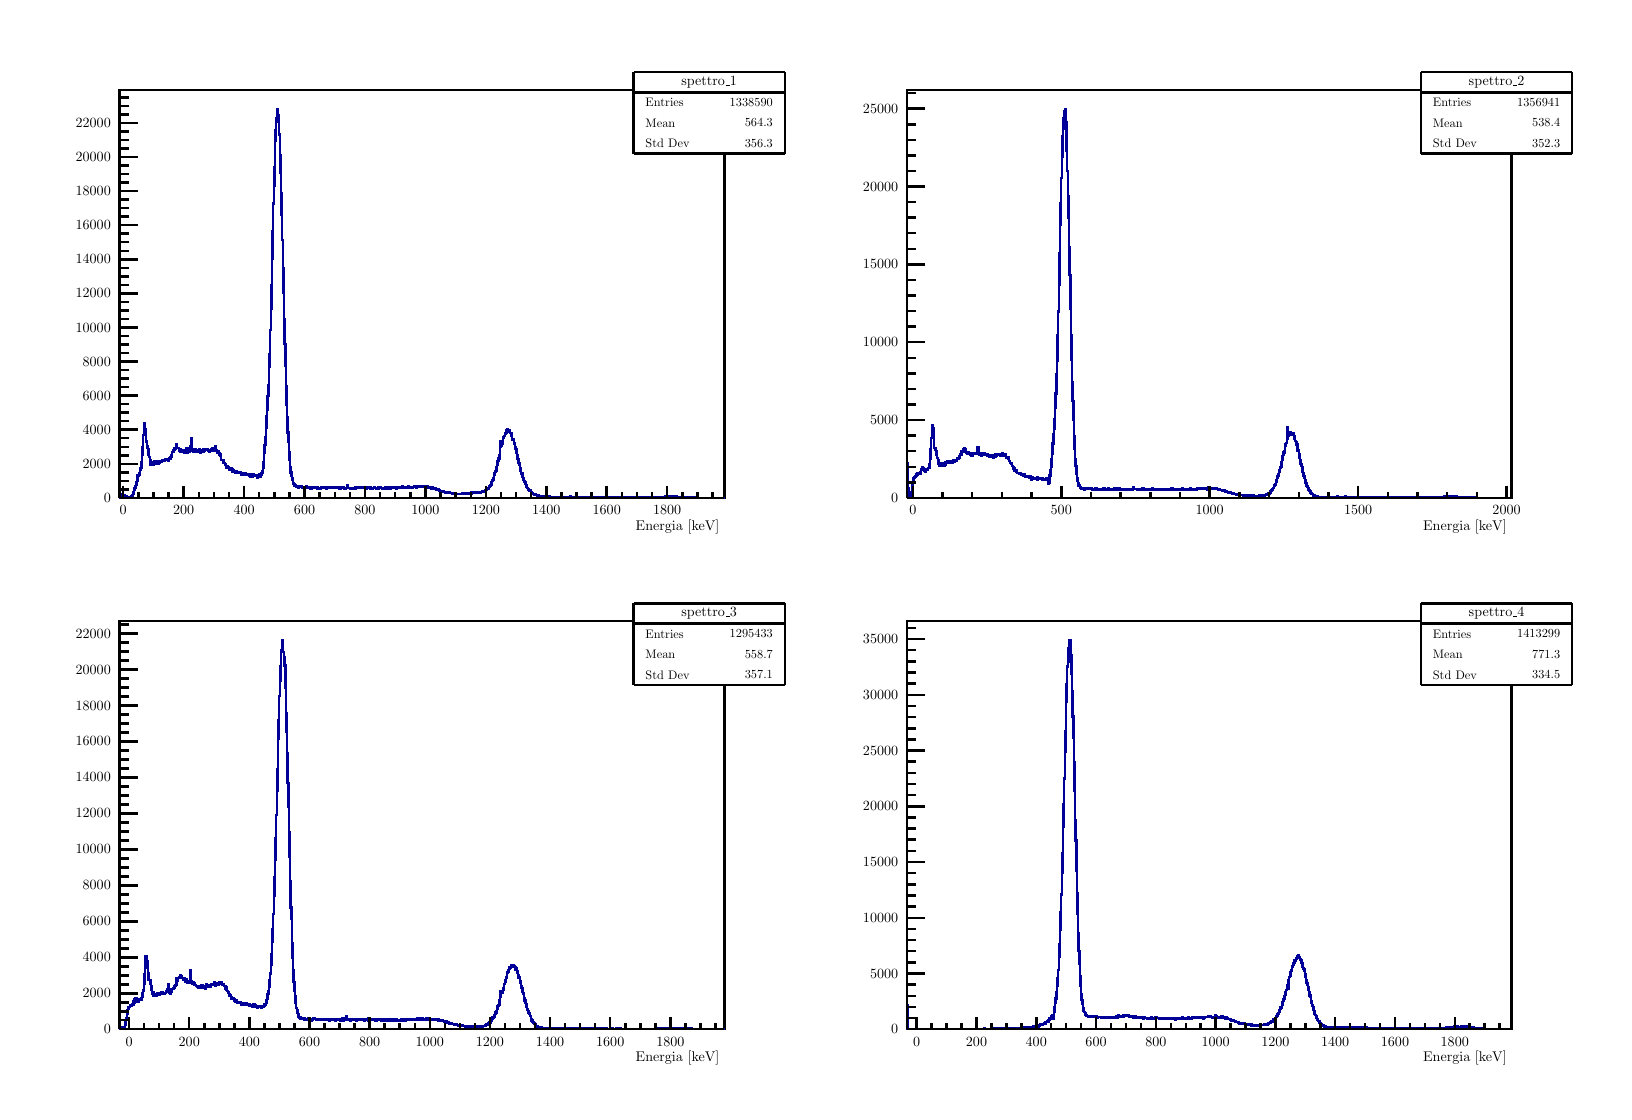
\begin{tikzpicture}
\pgfdeclareplotmark{cross} {
\pgfpathmoveto{\pgfpoint{-0.3\pgfplotmarksize}{\pgfplotmarksize}}
\pgfpathlineto{\pgfpoint{+0.3\pgfplotmarksize}{\pgfplotmarksize}}
\pgfpathlineto{\pgfpoint{+0.3\pgfplotmarksize}{0.3\pgfplotmarksize}}
\pgfpathlineto{\pgfpoint{+1\pgfplotmarksize}{0.3\pgfplotmarksize}}
\pgfpathlineto{\pgfpoint{+1\pgfplotmarksize}{-0.3\pgfplotmarksize}}
\pgfpathlineto{\pgfpoint{+0.3\pgfplotmarksize}{-0.3\pgfplotmarksize}}
\pgfpathlineto{\pgfpoint{+0.3\pgfplotmarksize}{-1.\pgfplotmarksize}}
\pgfpathlineto{\pgfpoint{-0.3\pgfplotmarksize}{-1.\pgfplotmarksize}}
\pgfpathlineto{\pgfpoint{-0.3\pgfplotmarksize}{-0.3\pgfplotmarksize}}
\pgfpathlineto{\pgfpoint{-1.\pgfplotmarksize}{-0.3\pgfplotmarksize}}
\pgfpathlineto{\pgfpoint{-1.\pgfplotmarksize}{0.3\pgfplotmarksize}}
\pgfpathlineto{\pgfpoint{-0.3\pgfplotmarksize}{0.3\pgfplotmarksize}}
\pgfpathclose
\pgfusepathqstroke
}
\pgfdeclareplotmark{cross*} {
\pgfpathmoveto{\pgfpoint{-0.3\pgfplotmarksize}{\pgfplotmarksize}}
\pgfpathlineto{\pgfpoint{+0.3\pgfplotmarksize}{\pgfplotmarksize}}
\pgfpathlineto{\pgfpoint{+0.3\pgfplotmarksize}{0.3\pgfplotmarksize}}
\pgfpathlineto{\pgfpoint{+1\pgfplotmarksize}{0.3\pgfplotmarksize}}
\pgfpathlineto{\pgfpoint{+1\pgfplotmarksize}{-0.3\pgfplotmarksize}}
\pgfpathlineto{\pgfpoint{+0.3\pgfplotmarksize}{-0.3\pgfplotmarksize}}
\pgfpathlineto{\pgfpoint{+0.3\pgfplotmarksize}{-1.\pgfplotmarksize}}
\pgfpathlineto{\pgfpoint{-0.3\pgfplotmarksize}{-1.\pgfplotmarksize}}
\pgfpathlineto{\pgfpoint{-0.3\pgfplotmarksize}{-0.3\pgfplotmarksize}}
\pgfpathlineto{\pgfpoint{-1.\pgfplotmarksize}{-0.3\pgfplotmarksize}}
\pgfpathlineto{\pgfpoint{-1.\pgfplotmarksize}{0.3\pgfplotmarksize}}
\pgfpathlineto{\pgfpoint{-0.3\pgfplotmarksize}{0.3\pgfplotmarksize}}
\pgfpathclose
\pgfusepathqfillstroke
}
\pgfdeclareplotmark{newstar} {
\pgfpathmoveto{\pgfqpoint{0pt}{\pgfplotmarksize}}
\pgfpathlineto{\pgfqpointpolar{44}{0.5\pgfplotmarksize}}
\pgfpathlineto{\pgfqpointpolar{18}{\pgfplotmarksize}}
\pgfpathlineto{\pgfqpointpolar{-20}{0.5\pgfplotmarksize}}
\pgfpathlineto{\pgfqpointpolar{-54}{\pgfplotmarksize}}
\pgfpathlineto{\pgfqpointpolar{-90}{0.5\pgfplotmarksize}}
\pgfpathlineto{\pgfqpointpolar{234}{\pgfplotmarksize}}
\pgfpathlineto{\pgfqpointpolar{198}{0.5\pgfplotmarksize}}
\pgfpathlineto{\pgfqpointpolar{162}{\pgfplotmarksize}}
\pgfpathlineto{\pgfqpointpolar{134}{0.5\pgfplotmarksize}}
\pgfpathclose
\pgfusepathqstroke
}
\pgfdeclareplotmark{newstar*} {
\pgfpathmoveto{\pgfqpoint{0pt}{\pgfplotmarksize}}
\pgfpathlineto{\pgfqpointpolar{44}{0.5\pgfplotmarksize}}
\pgfpathlineto{\pgfqpointpolar{18}{\pgfplotmarksize}}
\pgfpathlineto{\pgfqpointpolar{-20}{0.5\pgfplotmarksize}}
\pgfpathlineto{\pgfqpointpolar{-54}{\pgfplotmarksize}}
\pgfpathlineto{\pgfqpointpolar{-90}{0.5\pgfplotmarksize}}
\pgfpathlineto{\pgfqpointpolar{234}{\pgfplotmarksize}}
\pgfpathlineto{\pgfqpointpolar{198}{0.5\pgfplotmarksize}}
\pgfpathlineto{\pgfqpointpolar{162}{\pgfplotmarksize}}
\pgfpathlineto{\pgfqpointpolar{134}{0.5\pgfplotmarksize}}
\pgfpathclose
\pgfusepathqfillstroke
}
\definecolor{c}{rgb}{1,1,1};
\draw [color=c, fill=c] (0,0) rectangle (20,13.4957);
\draw [color=c, fill=c] (0.2,6.88281) rectangle (9.8,13.3607);
\draw [color=c, fill=c] (1.16,7.5306) rectangle (8.84,12.713);
\definecolor{c}{rgb}{0,0,0};
\draw [c,line width=0.9] (1.16,7.5306) -- (1.16,12.713) -- (8.84,12.713) -- (8.84,7.5306) -- (1.16,7.5306);
\definecolor{c}{rgb}{1,1,1};
\draw [color=c, fill=c] (1.16,7.5306) rectangle (8.84,12.713);
\definecolor{c}{rgb}{0,0,0};
\draw [c,line width=0.9] (1.16,7.5306) -- (1.16,12.713) -- (8.84,12.713) -- (8.84,7.5306) -- (1.16,7.5306);
\definecolor{c}{rgb}{0,0,0.6};
\draw [c,line width=0.9] (1.16,7.80379) -- (1.16768,7.80379) -- (1.16768,7.53125) -- (1.17536,7.53125) -- (1.17536,7.53147) -- (1.18304,7.53147) -- (1.18304,7.54229) -- (1.19072,7.54229) -- (1.19072,7.5661) -- (1.1984,7.5661) -- (1.1984,7.57195) --
 (1.20608,7.57195) -- (1.20608,7.5661) -- (1.21376,7.5661) -- (1.21376,7.56589) -- (1.22144,7.56589) -- (1.22144,7.55744) -- (1.22912,7.55744) -- (1.22912,7.55225) -- (1.2368,7.55225) -- (1.2368,7.54835) -- (1.24448,7.54835) -- (1.24448,7.54575) --
 (1.25216,7.54575) -- (1.25216,7.54337) -- (1.25984,7.54337) -- (1.25984,7.54337) -- (1.26752,7.54337) -- (1.26752,7.54056) -- (1.2752,7.54056) -- (1.2752,7.53991) -- (1.28288,7.53991) -- (1.28288,7.54272) -- (1.29056,7.54272) -- (1.29056,7.54099) --
 (1.29824,7.54099) -- (1.29824,7.54446) -- (1.30592,7.54446) -- (1.30592,7.55008) -- (1.3136,7.55008) -- (1.3136,7.55528) -- (1.32128,7.55528) -- (1.32128,7.56827) -- (1.32896,7.56827) -- (1.32896,7.58061) -- (1.33664,7.58061) -- (1.33664,7.60031) --
 (1.34432,7.60031) -- (1.34432,7.63364) -- (1.352,7.63364) -- (1.352,7.65464) -- (1.35968,7.65464) -- (1.35968,7.68127) -- (1.36736,7.68127) -- (1.36736,7.7001) -- (1.37504,7.7001) -- (1.37504,7.73365) -- (1.38272,7.73365) -- (1.38272,7.75465) --
 (1.3904,7.75465) -- (1.3904,7.81245) -- (1.39808,7.81245) -- (1.39808,7.8092) -- (1.40576,7.8092) -- (1.40576,7.82717) -- (1.41344,7.82717) -- (1.41344,7.84579) -- (1.42112,7.84579) -- (1.42112,7.88324) -- (1.4288,7.88324) -- (1.4288,7.90986) --
 (1.43648,7.90986) -- (1.43648,7.9826) -- (1.44416,7.9826) -- (1.44416,8.0733) -- (1.45184,8.0733) -- (1.45184,8.17872) -- (1.45952,8.17872) -- (1.45952,8.33155) -- (1.4672,8.33155) -- (1.4672,8.41511) -- (1.47488,8.41511) -- (1.47488,8.4846) --
 (1.48256,8.4846) -- (1.48256,8.39736) -- (1.49024,8.39736) -- (1.49024,8.33155) -- (1.49792,8.33155) -- (1.49792,8.24431) -- (1.5056,8.24431) -- (1.5056,8.18305) -- (1.51328,8.18305) -- (1.51328,8.16638) -- (1.52096,8.16638) -- (1.52096,8.14257) --
 (1.52864,8.14257) -- (1.52864,8.08109) -- (1.53632,8.08109) -- (1.53632,8.04905) -- (1.544,8.04905) -- (1.544,8.00792) -- (1.55168,8.00792) -- (1.55168,7.95467) -- (1.55936,7.95467) -- (1.55936,7.95684) -- (1.56704,7.95684) -- (1.56704,7.94666) --
 (1.57472,7.94666) -- (1.57472,7.94969) -- (1.5824,7.94969) -- (1.5824,7.98454) -- (1.59008,7.98454) -- (1.59008,7.95034) -- (1.59776,7.95034) -- (1.59776,7.97134) -- (1.60544,7.97134) -- (1.60544,7.99299) -- (1.61312,7.99299) -- (1.61312,7.96636) --
 (1.6208,7.96636) -- (1.6208,7.9826) -- (1.62848,7.9826) -- (1.62848,7.96073) -- (1.63616,7.96073) -- (1.63616,7.97718) -- (1.64384,7.97718) -- (1.64384,8.00056) -- (1.65152,8.00056) -- (1.65152,7.9642) -- (1.6592,7.9642) -- (1.6592,7.9787) --
 (1.66688,7.9787) -- (1.66688,7.99212) -- (1.67456,7.99212) -- (1.67456,7.99277) -- (1.68224,7.99277) -- (1.68224,7.99753) -- (1.68992,7.99753) -- (1.68992,7.99277) -- (1.6976,7.99277) -- (1.6976,8.0023) -- (1.70528,8.0023) -- (1.70528,8.01312) --
 (1.71296,8.01312) -- (1.71296,8.00338) -- (1.72064,8.00338) -- (1.72064,7.99688) -- (1.72832,7.99688) -- (1.72832,8.01182) -- (1.736,8.01182) -- (1.736,8.0155) -- (1.74368,8.0155) -- (1.74368,8.02373) -- (1.75136,8.02373) -- (1.75136,8.01442) --
 (1.75904,8.01442) -- (1.75904,8.01355) -- (1.76672,8.01355) -- (1.76672,8.0116) -- (1.7744,8.0116) -- (1.7744,8.02719) -- (1.78208,8.02719) -- (1.78208,8.00641) -- (1.78976,8.00641) -- (1.78976,8.03931) -- (1.79744,8.03931) -- (1.79744,8.03087) --
 (1.80512,8.03087) -- (1.80512,8.05143) -- (1.8128,8.05143) -- (1.8128,8.05879) -- (1.82048,8.05879) -- (1.82048,8.0733) -- (1.82816,8.0733) -- (1.82816,8.11421) -- (1.83584,8.11421) -- (1.83584,8.11508) -- (1.84352,8.11508) -- (1.84352,8.14105) --
 (1.8512,8.14105) -- (1.8512,8.16313) -- (1.85888,8.16313) -- (1.85888,8.14538) -- (1.86656,8.14538) -- (1.86656,8.15816) -- (1.87424,8.15816) -- (1.87424,8.19106) -- (1.88192,8.19106) -- (1.88192,8.21336) -- (1.8896,8.21336) -- (1.8896,8.1653) --
 (1.89728,8.1653) -- (1.89728,8.16746) -- (1.90496,8.16746) -- (1.90496,8.16184) -- (1.91264,8.16184) -- (1.91264,8.12504) -- (1.92032,8.12504) -- (1.92032,8.15015) -- (1.928,8.15015) -- (1.928,8.14668) -- (1.93568,8.14668) -- (1.93568,8.12222) --
 (1.94336,8.12222) -- (1.94336,8.13175) -- (1.95104,8.13175) -- (1.95104,8.13196) -- (1.95872,8.13196) -- (1.95872,8.12417) -- (1.9664,8.12417) -- (1.9664,8.12157) -- (1.97408,8.12157) -- (1.97408,8.12612) -- (1.98176,8.12612) -- (1.98176,8.10685) --
 (1.98944,8.10685) -- (1.98944,8.1298) -- (1.99712,8.1298) -- (1.99712,8.11335) -- (2.0048,8.11335) -- (2.0048,8.13759) -- (2.01248,8.13759) -- (2.01248,8.15621) -- (2.02016,8.15621) -- (2.02016,8.09992) -- (2.02784,8.09992) -- (2.02784,8.13456) --
 (2.03552,8.13456) -- (2.03552,8.12612) -- (2.0432,8.12612) -- (2.0432,8.11464) -- (2.05088,8.11464) -- (2.05088,8.14019) -- (2.05856,8.14019) -- (2.05856,8.1811) -- (2.06624,8.1811) -- (2.06624,8.29345) -- (2.07392,8.29345) -- (2.07392,8.1614) --
 (2.0816,8.1614) -- (2.0816,8.1482) -- (2.08928,8.1482) -- (2.08928,8.13543) -- (2.09696,8.13543) -- (2.09696,8.11313) -- (2.10464,8.11313) -- (2.10464,8.13499) -- (2.11232,8.13499) -- (2.11232,8.14127) -- (2.12,8.14127) -- (2.12,8.15015) --
 (2.12768,8.15015) -- (2.12768,8.13932) -- (2.13536,8.13932) -- (2.13536,8.11421) -- (2.14304,8.11421) -- (2.14304,8.11897) -- (2.15072,8.11897) -- (2.15072,8.13781) -- (2.1584,8.13781) -- (2.1584,8.1417) -- (2.16608,8.1417) -- (2.16608,8.14452) --
 (2.17376,8.14452) -- (2.17376,8.13543) -- (2.18144,8.13543) -- (2.18144,8.10707) -- (2.18912,8.10707) -- (2.18912,8.12677) -- (2.1968,8.12677) -- (2.1968,8.12244) -- (2.20448,8.12244) -- (2.20448,8.11616) -- (2.21216,8.11616) -- (2.21216,8.13543) --
 (2.21984,8.13543) -- (2.21984,8.1443) -- (2.22752,8.1443) -- (2.22752,8.11486) -- (2.2352,8.11486) -- (2.2352,8.12374) -- (2.24288,8.12374) -- (2.24288,8.14387) -- (2.25056,8.14387) -- (2.25056,8.13651) -- (2.25824,8.13651) -- (2.25824,8.14019) --
 (2.26592,8.14019) -- (2.26592,8.14538) -- (2.2736,8.14538) -- (2.2736,8.14495) -- (2.28128,8.14495) -- (2.28128,8.1272) -- (2.28896,8.1272) -- (2.28896,8.13326) -- (2.29664,8.13326) -- (2.29664,8.11962) -- (2.30432,8.11962) -- (2.30432,8.13802) --
 (2.312,8.13802) -- (2.312,8.13239) -- (2.31968,8.13239) -- (2.31968,8.14603) -- (2.32736,8.14603) -- (2.32736,8.13694) -- (2.33504,8.13694) -- (2.33504,8.15794) -- (2.34272,8.15794) -- (2.34272,8.13456) -- (2.3504,8.13456) -- (2.3504,8.14538) --
 (2.35808,8.14538) -- (2.35808,8.14625) -- (2.36576,8.14625) -- (2.36576,8.14993) -- (2.37344,8.14993) -- (2.37344,8.1811) -- (2.38112,8.1811) -- (2.38112,8.1298) -- (2.3888,8.1298) -- (2.3888,8.1246) -- (2.39648,8.1246) -- (2.39648,8.10469) --
 (2.40416,8.10469) -- (2.40416,8.12698) -- (2.41184,8.12698) -- (2.41184,8.12395) -- (2.41952,8.12395) -- (2.41952,8.10404) -- (2.4272,8.10404) -- (2.4272,8.08087) -- (2.43488,8.08087) -- (2.43488,8.0891) -- (2.44256,8.0891) -- (2.44256,8.06053) --
 (2.45024,8.06053) -- (2.45024,8.0129) -- (2.45792,8.0129) -- (2.45792,8.00944) -- (2.4656,8.00944) -- (2.4656,8.01398) -- (2.47328,8.01398) -- (2.47328,8.0116) -- (2.48096,8.0116) -- (2.48096,7.97307) -- (2.48864,7.97307) -- (2.48864,7.97589) --
 (2.49632,7.97589) -- (2.49632,7.96225) -- (2.504,7.96225) -- (2.504,7.94839) -- (2.51168,7.94839) -- (2.51168,7.92826) -- (2.51936,7.92826) -- (2.51936,7.91917) -- (2.52704,7.91917) -- (2.52704,7.93021) -- (2.53472,7.93021) -- (2.53472,7.9235) --
 (2.5424,7.9235) -- (2.5424,7.91679) -- (2.55008,7.91679) -- (2.55008,7.9025) -- (2.55776,7.9025) -- (2.55776,7.89428) -- (2.56544,7.89428) -- (2.56544,7.89341) -- (2.57312,7.89341) -- (2.57312,7.90337) -- (2.5808,7.90337) -- (2.5808,7.88194) --
 (2.58848,7.88194) -- (2.58848,7.89536) -- (2.59616,7.89536) -- (2.59616,7.85877) -- (2.60384,7.85877) -- (2.60384,7.88388) -- (2.61152,7.88388) -- (2.61152,7.87436) -- (2.6192,7.87436) -- (2.6192,7.86029) -- (2.62688,7.86029) -- (2.62688,7.86462) --
 (2.63456,7.86462) -- (2.63456,7.84557) -- (2.64224,7.84557) -- (2.64224,7.86548) -- (2.64992,7.86548) -- (2.64992,7.85812) -- (2.6576,7.85812) -- (2.6576,7.85618) -- (2.66528,7.85618) -- (2.66528,7.84687) -- (2.67296,7.84687) -- (2.67296,7.85704) --
 (2.68064,7.85704) -- (2.68064,7.84947) -- (2.68832,7.84947) -- (2.68832,7.85769) -- (2.696,7.85769) -- (2.696,7.85401) -- (2.70368,7.85401) -- (2.70368,7.83886) -- (2.71136,7.83886) -- (2.71136,7.82803) -- (2.71904,7.82803) -- (2.71904,7.83972) --
 (2.72672,7.83972) -- (2.72672,7.83518) -- (2.7344,7.83518) -- (2.7344,7.84124) -- (2.74208,7.84124) -- (2.74208,7.83085) -- (2.74976,7.83085) -- (2.74976,7.83756) -- (2.75744,7.83756) -- (2.75744,7.84037) -- (2.76512,7.84037) -- (2.76512,7.83475) --
 (2.7728,7.83475) -- (2.7728,7.8289) -- (2.78048,7.8289) -- (2.78048,7.8276) -- (2.78816,7.8276) -- (2.78816,7.82609) -- (2.79584,7.82609) -- (2.79584,7.8289) -- (2.80352,7.8289) -- (2.80352,7.81764) -- (2.8112,7.81764) -- (2.8112,7.81743) --
 (2.81888,7.81743) -- (2.81888,7.80487) -- (2.82656,7.80487) -- (2.82656,7.81764) -- (2.83424,7.81764) -- (2.83424,7.8302) -- (2.84192,7.8302) -- (2.84192,7.80098) -- (2.8496,7.80098) -- (2.8496,7.81266) -- (2.85728,7.81266) -- (2.85728,7.82868) --
 (2.86496,7.82868) -- (2.86496,7.82089) -- (2.87264,7.82089) -- (2.87264,7.80855) -- (2.88032,7.80855) -- (2.88032,7.80963) -- (2.888,7.80963) -- (2.888,7.82132) -- (2.89568,7.82132) -- (2.89568,7.82306) -- (2.90336,7.82306) -- (2.90336,7.78994) --
 (2.91104,7.78994) -- (2.91104,7.80292) -- (2.91872,7.80292) -- (2.91872,7.80834) -- (2.9264,7.80834) -- (2.9264,7.80704) -- (2.93408,7.80704) -- (2.93408,7.82998) -- (2.94176,7.82998) -- (2.94176,7.80271) -- (2.94944,7.80271) -- (2.94944,7.82067) --
 (2.95712,7.82067) -- (2.95712,7.82825) -- (2.9648,7.82825) -- (2.9648,7.8473) -- (2.97248,7.8473) -- (2.97248,7.87371) -- (2.98016,7.87371) -- (2.98016,7.91462) -- (2.98784,7.91462) -- (2.98784,7.98433) -- (2.99552,7.98433) -- (2.99552,8.10079) --
 (3.0032,8.10079) -- (3.0032,8.2008) -- (3.01088,8.2008) -- (3.01088,8.30362) -- (3.01856,8.30362) -- (3.01856,8.42615) -- (3.02624,8.42615) -- (3.02624,8.56469) -- (3.03392,8.56469) -- (3.03392,8.65409) -- (3.0416,8.65409) -- (3.0416,8.82381) --
 (3.04928,8.82381) -- (3.04928,8.96192) -- (3.05696,8.96192) -- (3.05696,9.2022) -- (3.06464,9.2022) -- (3.06464,9.35178) -- (3.07232,9.35178) -- (3.07232,9.66459) -- (3.08,9.66459) -- (3.08,9.93756) -- (3.08768,9.93756) -- (3.08768,10.2313) --
 (3.09536,10.2313) -- (3.09536,10.5675) -- (3.10304,10.5675) -- (3.10304,10.9195) -- (3.11072,10.9195) -- (3.11072,11.2693) -- (3.1184,11.2693) -- (3.1184,11.4912) -- (3.12608,11.4912) -- (3.12608,11.7341) -- (3.13376,11.7341) -- (3.13376,12.072) --
 (3.14144,12.072) -- (3.14144,12.2003) -- (3.14912,12.2003) -- (3.14912,12.3545) -- (3.1568,12.3545) -- (3.1568,12.3952) -- (3.16448,12.3952) -- (3.16448,12.4662) -- (3.17216,12.4662) -- (3.17216,12.309) -- (3.17984,12.309) -- (3.17984,12.3874) --
 (3.18752,12.3874) -- (3.18752,12.1475) -- (3.1952,12.1475) -- (3.1952,11.8761) -- (3.20288,11.8761) -- (3.20288,11.6585) -- (3.21056,11.6585) -- (3.21056,11.4052) -- (3.21824,11.4052) -- (3.21824,11.1217) -- (3.22592,11.1217) -- (3.22592,10.8076) --
 (3.2336,10.8076) -- (3.2336,10.445) -- (3.24128,10.445) -- (3.24128,10.1397) -- (3.24896,10.1397) -- (3.24896,9.7949) -- (3.25664,9.7949) -- (3.25664,9.48232) -- (3.26432,9.48232) -- (3.26432,9.20631) -- (3.272,9.20631) -- (3.272,8.95066) --
 (3.27968,8.95066) -- (3.27968,8.71839) -- (3.28736,8.71839) -- (3.28736,8.55084) -- (3.29504,8.55084) -- (3.29504,8.36229) -- (3.30272,8.36229) -- (3.30272,8.23868) -- (3.3104,8.23868) -- (3.3104,8.1062) -- (3.31808,8.1062) -- (3.31808,8.01312) --
 (3.32576,8.01312) -- (3.32576,7.9261) -- (3.33344,7.9261) -- (3.33344,7.85509) -- (3.34112,7.85509) -- (3.34112,7.81829) -- (3.3488,7.81829) -- (3.3488,7.77413) -- (3.35648,7.77413) -- (3.35648,7.7553) -- (3.36416,7.7553) -- (3.36416,7.72153) --
 (3.37184,7.72153) -- (3.37184,7.70984) -- (3.37952,7.70984) -- (3.37952,7.68473) -- (3.3872,7.68473) -- (3.3872,7.69057) -- (3.39488,7.69057) -- (3.39488,7.68473) -- (3.40256,7.68473) -- (3.40256,7.67304) -- (3.41024,7.67304) -- (3.41024,7.68408) --
 (3.41792,7.68408) -- (3.41792,7.67261) -- (3.4256,7.67261) -- (3.4256,7.67607) -- (3.43328,7.67607) -- (3.43328,7.66525) -- (3.44096,7.66525) -- (3.44096,7.67282) -- (3.44864,7.67282) -- (3.44864,7.66871) -- (3.45632,7.66871) -- (3.45632,7.66828) --
 (3.464,7.66828) -- (3.464,7.67282) -- (3.47168,7.67282) -- (3.47168,7.66849) -- (3.47936,7.66849) -- (3.47936,7.65681) -- (3.48704,7.65681) -- (3.48704,7.67109) -- (3.49472,7.67109) -- (3.49472,7.66135) -- (3.5024,7.66135) -- (3.5024,7.6659) --
 (3.51008,7.6659) -- (3.51008,7.66546) -- (3.51776,7.66546) -- (3.51776,7.66352) -- (3.52544,7.66352) -- (3.52544,7.67607) -- (3.53312,7.67607) -- (3.53312,7.66135) -- (3.5408,7.66135) -- (3.5408,7.65745) -- (3.54848,7.65745) -- (3.54848,7.66178) --
 (3.55616,7.66178) -- (3.55616,7.66308) -- (3.56384,7.66308) -- (3.56384,7.66546) -- (3.57152,7.66546) -- (3.57152,7.65659) -- (3.5792,7.65659) -- (3.5792,7.66135) -- (3.58688,7.66135) -- (3.58688,7.65204) -- (3.59456,7.65204) -- (3.59456,7.6607) --
 (3.60224,7.6607) -- (3.60224,7.65767) -- (3.60992,7.65767) -- (3.60992,7.65984) -- (3.6176,7.65984) -- (3.6176,7.65745) -- (3.62528,7.65745) -- (3.62528,7.66373) -- (3.63296,7.66373) -- (3.63296,7.66611) -- (3.64064,7.66611) -- (3.64064,7.65399) --
 (3.64832,7.65399) -- (3.64832,7.66222) -- (3.656,7.66222) -- (3.656,7.65962) -- (3.66368,7.65962) -- (3.66368,7.66049) -- (3.67136,7.66049) -- (3.67136,7.65226) -- (3.67904,7.65226) -- (3.67904,7.65875) -- (3.68672,7.65875) -- (3.68672,7.65139) --
 (3.6944,7.65139) -- (3.6944,7.65854) -- (3.70208,7.65854) -- (3.70208,7.64338) -- (3.70976,7.64338) -- (3.70976,7.65269) -- (3.71744,7.65269) -- (3.71744,7.66092) -- (3.72512,7.66092) -- (3.72512,7.662) -- (3.7328,7.662) -- (3.7328,7.65356) --
 (3.74048,7.65356) -- (3.74048,7.65919) -- (3.74816,7.65919) -- (3.74816,7.67131) -- (3.75584,7.67131) -- (3.75584,7.65616) -- (3.76352,7.65616) -- (3.76352,7.66395) -- (3.7712,7.66395) -- (3.7712,7.66785) -- (3.77888,7.66785) -- (3.77888,7.65356) --
 (3.78656,7.65356) -- (3.78656,7.6475) -- (3.79424,7.6475) -- (3.79424,7.66655) -- (3.80192,7.66655) -- (3.80192,7.66373) -- (3.8096,7.66373) -- (3.8096,7.65724) -- (3.81728,7.65724) -- (3.81728,7.6646) -- (3.82496,7.6646) -- (3.82496,7.65551) --
 (3.83264,7.65551) -- (3.83264,7.65377) -- (3.84032,7.65377) -- (3.84032,7.66395) -- (3.848,7.66395) -- (3.848,7.6607) -- (3.85568,7.6607) -- (3.85568,7.65616) -- (3.86336,7.65616) -- (3.86336,7.6646) -- (3.87104,7.6646) -- (3.87104,7.66113) --
 (3.87872,7.66113) -- (3.87872,7.66525) -- (3.8864,7.66525) -- (3.8864,7.65356) -- (3.89408,7.65356) -- (3.89408,7.66005) -- (3.90176,7.66005) -- (3.90176,7.65356) -- (3.90944,7.65356) -- (3.90944,7.65789) -- (3.91712,7.65789) -- (3.91712,7.65745) --
 (3.9248,7.65745) -- (3.9248,7.65421) -- (3.93248,7.65421) -- (3.93248,7.66503) -- (3.94016,7.66503) -- (3.94016,7.65789) -- (3.94784,7.65789) -- (3.94784,7.64728) -- (3.95552,7.64728) -- (3.95552,7.65118) -- (3.9632,7.65118) -- (3.9632,7.65897) --
 (3.97088,7.65897) -- (3.97088,7.65745) -- (3.97856,7.65745) -- (3.97856,7.66005) -- (3.98624,7.66005) -- (3.98624,7.65681) -- (3.99392,7.65681) -- (3.99392,7.66135) -- (4.0016,7.66135) -- (4.0016,7.65529) -- (4.00928,7.65529) -- (4.00928,7.65248) --
 (4.01696,7.65248) -- (4.01696,7.65421) -- (4.02464,7.65421) -- (4.02464,7.6449) -- (4.03232,7.6449) -- (4.03232,7.65854) -- (4.04,7.65854) -- (4.04,7.65702) -- (4.04768,7.65702) -- (4.04768,7.66893) -- (4.05536,7.66893) -- (4.05536,7.69187) --
 (4.06304,7.69187) -- (4.06304,7.65659) -- (4.07072,7.65659) -- (4.07072,7.65637) -- (4.0784,7.65637) -- (4.0784,7.65789) -- (4.08608,7.65789) -- (4.08608,7.65313) -- (4.09376,7.65313) -- (4.09376,7.65789) -- (4.10144,7.65789) -- (4.10144,7.65356) --
 (4.10912,7.65356) -- (4.10912,7.65767) -- (4.1168,7.65767) -- (4.1168,7.65291) -- (4.12448,7.65291) -- (4.12448,7.65269) -- (4.13216,7.65269) -- (4.13216,7.64576) -- (4.13984,7.64576) -- (4.13984,7.65767) -- (4.14752,7.65767) -- (4.14752,7.66503) --
 (4.1552,7.66503) -- (4.1552,7.65269) -- (4.16288,7.65269) -- (4.16288,7.65854) -- (4.17056,7.65854) -- (4.17056,7.66265) -- (4.17824,7.66265) -- (4.17824,7.66157) -- (4.18592,7.66157) -- (4.18592,7.66308) -- (4.1936,7.66308) -- (4.1936,7.65681) --
 (4.20128,7.65681) -- (4.20128,7.65962) -- (4.20896,7.65962) -- (4.20896,7.66698) -- (4.21664,7.66698) -- (4.21664,7.66849) -- (4.22432,7.66849) -- (4.22432,7.65572) -- (4.232,7.65572) -- (4.232,7.65637) -- (4.23968,7.65637) -- (4.23968,7.65486) --
 (4.24736,7.65486) -- (4.24736,7.65702) -- (4.25504,7.65702) -- (4.25504,7.66243) -- (4.26272,7.66243) -- (4.26272,7.66849) -- (4.2704,7.66849) -- (4.2704,7.65356) -- (4.27808,7.65356) -- (4.27808,7.64901) -- (4.28576,7.64901) -- (4.28576,7.6607) --
 (4.29344,7.6607) -- (4.29344,7.65139) -- (4.30112,7.65139) -- (4.30112,7.662) -- (4.3088,7.662) -- (4.3088,7.65442) -- (4.31648,7.65442) -- (4.31648,7.65789) -- (4.32416,7.65789) -- (4.32416,7.65377) -- (4.33184,7.65377) -- (4.33184,7.66893) --
 (4.33952,7.66893) -- (4.33952,7.66655) -- (4.3472,7.66655) -- (4.3472,7.65139) -- (4.35488,7.65139) -- (4.35488,7.65204) -- (4.36256,7.65204) -- (4.36256,7.65551) -- (4.37024,7.65551) -- (4.37024,7.64815) -- (4.37792,7.64815) -- (4.37792,7.65616) --
 (4.3856,7.65616) -- (4.3856,7.65659) -- (4.39328,7.65659) -- (4.39328,7.66525) -- (4.40096,7.66525) -- (4.40096,7.65356) -- (4.40864,7.65356) -- (4.40864,7.65767) -- (4.41632,7.65767) -- (4.41632,7.6462) -- (4.424,7.6462) -- (4.424,7.65442) --
 (4.43168,7.65442) -- (4.43168,7.65897) -- (4.43936,7.65897) -- (4.43936,7.64836) -- (4.44704,7.64836) -- (4.44704,7.66438) -- (4.45472,7.66438) -- (4.45472,7.66395) -- (4.4624,7.66395) -- (4.4624,7.66914) -- (4.47008,7.66914) -- (4.47008,7.65984) --
 (4.47776,7.65984) -- (4.47776,7.65572) -- (4.48544,7.65572) -- (4.48544,7.65875) -- (4.49312,7.65875) -- (4.49312,7.64728) -- (4.5008,7.64728) -- (4.5008,7.6462) -- (4.50848,7.6462) -- (4.50848,7.65074) -- (4.51616,7.65074) -- (4.51616,7.65529) --
 (4.52384,7.65529) -- (4.52384,7.65919) -- (4.53152,7.65919) -- (4.53152,7.662) -- (4.5392,7.662) -- (4.5392,7.6462) -- (4.54688,7.6462) -- (4.54688,7.64923) -- (4.55456,7.64923) -- (4.55456,7.66785) -- (4.56224,7.66785) -- (4.56224,7.65118) --
 (4.56992,7.65118) -- (4.56992,7.662) -- (4.5776,7.662) -- (4.5776,7.66113) -- (4.58528,7.66113) -- (4.58528,7.6594) -- (4.59296,7.6594) -- (4.59296,7.65313) -- (4.60064,7.65313) -- (4.60064,7.65702) -- (4.60832,7.65702) -- (4.60832,7.66135) --
 (4.616,7.66135) -- (4.616,7.6633) -- (4.62368,7.6633) -- (4.62368,7.6607) -- (4.63136,7.6607) -- (4.63136,7.66092) -- (4.63904,7.66092) -- (4.63904,7.66438) -- (4.64672,7.66438) -- (4.64672,7.65789) -- (4.6544,7.65789) -- (4.6544,7.66222) --
 (4.66208,7.66222) -- (4.66208,7.66417) -- (4.66976,7.66417) -- (4.66976,7.64966) -- (4.67744,7.64966) -- (4.67744,7.65724) -- (4.68512,7.65724) -- (4.68512,7.65745) -- (4.6928,7.65745) -- (4.6928,7.66005) -- (4.70048,7.66005) -- (4.70048,7.65659) --
 (4.70816,7.65659) -- (4.70816,7.66092) -- (4.71584,7.66092) -- (4.71584,7.66222) -- (4.72352,7.66222) -- (4.72352,7.65919) -- (4.7312,7.65919) -- (4.7312,7.65724) -- (4.73888,7.65724) -- (4.73888,7.66049) -- (4.74656,7.66049) -- (4.74656,7.6633) --
 (4.75424,7.6633) -- (4.75424,7.67304) -- (4.76192,7.67304) -- (4.76192,7.66287) -- (4.7696,7.66287) -- (4.7696,7.66611) -- (4.77728,7.66611) -- (4.77728,7.662) -- (4.78496,7.662) -- (4.78496,7.66525) -- (4.79264,7.66525) -- (4.79264,7.65572) --
 (4.80032,7.65572) -- (4.80032,7.662) -- (4.808,7.662) -- (4.808,7.6659) -- (4.81568,7.6659) -- (4.81568,7.6594) -- (4.82336,7.6594) -- (4.82336,7.67521) -- (4.83104,7.67521) -- (4.83104,7.67629) -- (4.83872,7.67629) -- (4.83872,7.66893) --
 (4.8464,7.66893) -- (4.8464,7.67196) -- (4.85408,7.67196) -- (4.85408,7.65875) -- (4.86176,7.65875) -- (4.86176,7.6659) -- (4.86944,7.6659) -- (4.86944,7.66178) -- (4.87712,7.66178) -- (4.87712,7.66417) -- (4.8848,7.66417) -- (4.8848,7.66849) --
 (4.89248,7.66849) -- (4.89248,7.67088) -- (4.90016,7.67088) -- (4.90016,7.66828) -- (4.90784,7.66828) -- (4.90784,7.6791) -- (4.91552,7.6791) -- (4.91552,7.67217) -- (4.9232,7.67217) -- (4.9232,7.6646) -- (4.93088,7.6646) -- (4.93088,7.66958) --
 (4.93856,7.66958) -- (4.93856,7.67932) -- (4.94624,7.67932) -- (4.94624,7.67456) -- (4.95392,7.67456) -- (4.95392,7.67066) -- (4.9616,7.67066) -- (4.9616,7.67044) -- (4.96928,7.67044) -- (4.96928,7.66655) -- (4.97696,7.66655) -- (4.97696,7.67044) --
 (4.98464,7.67044) -- (4.98464,7.67845) -- (4.99232,7.67845) -- (4.99232,7.67109) -- (5,7.67109) -- (5,7.67391) -- (5.00768,7.67391) -- (5.00768,7.67261) -- (5.01536,7.67261) -- (5.01536,7.66828) -- (5.02304,7.66828) -- (5.02304,7.66633) --
 (5.03072,7.66633) -- (5.03072,7.67304) -- (5.0384,7.67304) -- (5.0384,7.67088) -- (5.04608,7.67088) -- (5.04608,7.67023) -- (5.05376,7.67023) -- (5.05376,7.66417) -- (5.06144,7.66417) -- (5.06144,7.67326) -- (5.06912,7.67326) -- (5.06912,7.6659) --
 (5.0768,7.6659) -- (5.0768,7.6672) -- (5.08448,7.6672) -- (5.08448,7.66005) -- (5.09216,7.66005) -- (5.09216,7.66005) -- (5.09984,7.66005) -- (5.09984,7.65984) -- (5.10752,7.65984) -- (5.10752,7.6633) -- (5.1152,7.6633) -- (5.1152,7.66352) --
 (5.12288,7.66352) -- (5.12288,7.64988) -- (5.13056,7.64988) -- (5.13056,7.66157) -- (5.13824,7.66157) -- (5.13824,7.65356) -- (5.14592,7.65356) -- (5.14592,7.65594) -- (5.1536,7.65594) -- (5.1536,7.65074) -- (5.16128,7.65074) -- (5.16128,7.65139) --
 (5.16896,7.65139) -- (5.16896,7.6475) -- (5.17664,7.6475) -- (5.17664,7.64338) -- (5.18432,7.64338) -- (5.18432,7.63732) -- (5.192,7.63732) -- (5.192,7.64641) -- (5.19968,7.64641) -- (5.19968,7.63949) -- (5.20736,7.63949) -- (5.20736,7.64273) --
 (5.21504,7.64273) -- (5.21504,7.63213) -- (5.22272,7.63213) -- (5.22272,7.62715) -- (5.2304,7.62715) -- (5.2304,7.62022) -- (5.23808,7.62022) -- (5.23808,7.62) -- (5.24576,7.62) -- (5.24576,7.62022) -- (5.25344,7.62022) -- (5.25344,7.61892) --
 (5.26112,7.61892) -- (5.26112,7.61849) -- (5.2688,7.61849) -- (5.2688,7.61459) -- (5.27648,7.61459) -- (5.27648,7.60399) -- (5.28416,7.60399) -- (5.28416,7.60334) -- (5.29184,7.60334) -- (5.29184,7.60723) -- (5.29952,7.60723) -- (5.29952,7.60225) --
 (5.3072,7.60225) -- (5.3072,7.59922) -- (5.31488,7.59922) -- (5.31488,7.60334) -- (5.32256,7.60334) -- (5.32256,7.60377) -- (5.33024,7.60377) -- (5.33024,7.59814) -- (5.33792,7.59814) -- (5.33792,7.59641) -- (5.3456,7.59641) -- (5.3456,7.59749) --
 (5.35328,7.59749) -- (5.35328,7.591) -- (5.36096,7.591) -- (5.36096,7.59121) -- (5.36864,7.59121) -- (5.36864,7.59251) -- (5.37632,7.59251) -- (5.37632,7.59035) -- (5.384,7.59035) -- (5.384,7.5884) -- (5.39168,7.5884) -- (5.39168,7.59121) --
 (5.39936,7.59121) -- (5.39936,7.58775) -- (5.40704,7.58775) -- (5.40704,7.5858) -- (5.41472,7.5858) -- (5.41472,7.591) -- (5.4224,7.591) -- (5.4224,7.5884) -- (5.43008,7.5884) -- (5.43008,7.58126) -- (5.43776,7.58126) -- (5.43776,7.58082) --
 (5.44544,7.58082) -- (5.44544,7.58017) -- (5.45312,7.58017) -- (5.45312,7.57714) -- (5.4608,7.57714) -- (5.4608,7.58169) -- (5.46848,7.58169) -- (5.46848,7.58277) -- (5.47616,7.58277) -- (5.47616,7.57952) -- (5.48384,7.57952) -- (5.48384,7.57801) --
 (5.49152,7.57801) -- (5.49152,7.57736) -- (5.4992,7.57736) -- (5.4992,7.58299) -- (5.50688,7.58299) -- (5.50688,7.57952) -- (5.51456,7.57952) -- (5.51456,7.58429) -- (5.52224,7.58429) -- (5.52224,7.57801) -- (5.52992,7.57801) -- (5.52992,7.58342) --
 (5.5376,7.58342) -- (5.5376,7.58753) -- (5.54528,7.58753) -- (5.54528,7.58191) -- (5.55296,7.58191) -- (5.55296,7.58342) -- (5.56064,7.58342) -- (5.56064,7.58948) -- (5.56832,7.58948) -- (5.56832,7.58732) -- (5.576,7.58732) -- (5.576,7.58494) --
 (5.58368,7.58494) -- (5.58368,7.58472) -- (5.59136,7.58472) -- (5.59136,7.58797) -- (5.59904,7.58797) -- (5.59904,7.58992) -- (5.60672,7.58992) -- (5.60672,7.58429) -- (5.6144,7.58429) -- (5.6144,7.5936) -- (5.62208,7.5936) -- (5.62208,7.59944) --
 (5.62976,7.59944) -- (5.62976,7.58753) -- (5.63744,7.58753) -- (5.63744,7.60009) -- (5.64512,7.60009) -- (5.64512,7.59013) -- (5.6528,7.59013) -- (5.6528,7.59641) -- (5.66048,7.59641) -- (5.66048,7.59273) -- (5.66816,7.59273) -- (5.66816,7.59576) --
 (5.67584,7.59576) -- (5.67584,7.60464) -- (5.68352,7.60464) -- (5.68352,7.59598) -- (5.6912,7.59598) -- (5.6912,7.59728) -- (5.69888,7.59728) -- (5.69888,7.59879) -- (5.70656,7.59879) -- (5.70656,7.59706) -- (5.71424,7.59706) -- (5.71424,7.59987) --
 (5.72192,7.59987) -- (5.72192,7.6016) -- (5.7296,7.6016) -- (5.7296,7.60096) -- (5.73728,7.60096) -- (5.73728,7.60031) -- (5.74496,7.60031) -- (5.74496,7.60269) -- (5.75264,7.60269) -- (5.75264,7.60334) -- (5.76032,7.60334) -- (5.76032,7.61264) --
 (5.768,7.61264) -- (5.768,7.60442) -- (5.77568,7.60442) -- (5.77568,7.6107) -- (5.78336,7.6107) -- (5.78336,7.61459) -- (5.79104,7.61459) -- (5.79104,7.60896) -- (5.79872,7.60896) -- (5.79872,7.61892) -- (5.8064,7.61892) -- (5.8064,7.63364) --
 (5.81408,7.63364) -- (5.81408,7.63083) -- (5.82176,7.63083) -- (5.82176,7.63537) -- (5.82944,7.63537) -- (5.82944,7.6462) -- (5.83712,7.6462) -- (5.83712,7.64771) -- (5.8448,7.64771) -- (5.8448,7.65399) -- (5.85248,7.65399) -- (5.85248,7.67066) --
 (5.86016,7.67066) -- (5.86016,7.68408) -- (5.86784,7.68408) -- (5.86784,7.69555) -- (5.87552,7.69555) -- (5.87552,7.70226) -- (5.8832,7.70226) -- (5.8832,7.72889) -- (5.89088,7.72889) -- (5.89088,7.74448) -- (5.89856,7.74448) -- (5.89856,7.75898) --
 (5.90624,7.75898) -- (5.90624,7.78582) -- (5.91392,7.78582) -- (5.91392,7.82089) -- (5.9216,7.82089) -- (5.9216,7.83799) -- (5.92928,7.83799) -- (5.92928,7.86354) -- (5.93696,7.86354) -- (5.93696,7.87371) -- (5.94464,7.87371) -- (5.94464,7.91679) --
 (5.95232,7.91679) -- (5.95232,7.95164) -- (5.96,7.95164) -- (5.96,7.99234) -- (5.96768,7.99234) -- (5.96768,8.00424) -- (5.97536,8.00424) -- (5.97536,8.0287) -- (5.98304,8.0287) -- (5.98304,8.06854) -- (5.99072,8.06854) -- (5.99072,8.17959) --
 (5.9984,8.17959) -- (5.9984,8.25427) -- (6.00608,8.25427) -- (6.00608,8.1969) -- (6.01376,8.1969) -- (6.01376,8.22007) -- (6.02144,8.22007) -- (6.02144,8.22894) -- (6.02912,8.22894) -- (6.02912,8.29367) -- (6.0368,8.29367) -- (6.0368,8.30427) --
 (6.04448,8.30427) -- (6.04448,8.31964) -- (6.05216,8.31964) -- (6.05216,8.34973) -- (6.05984,8.34973) -- (6.05984,8.35147) -- (6.06752,8.35147) -- (6.06752,8.35276) -- (6.0752,8.35276) -- (6.0752,8.39281) -- (6.08288,8.39281) -- (6.08288,8.39844) --
 (6.09056,8.39844) -- (6.09056,8.36965) -- (6.09824,8.36965) -- (6.09824,8.39541) -- (6.10592,8.39541) -- (6.10592,8.38588) -- (6.1136,8.38588) -- (6.1136,8.38545) -- (6.12128,8.38545) -- (6.12128,8.35601) -- (6.12896,8.35601) -- (6.12896,8.348) --
 (6.13664,8.348) -- (6.13664,8.32289) -- (6.14432,8.32289) -- (6.14432,8.27267) -- (6.152,8.27267) -- (6.152,8.26661) -- (6.15968,8.26661) -- (6.15968,8.27159) -- (6.16736,8.27159) -- (6.16736,8.22526) -- (6.17504,8.22526) -- (6.17504,8.21487) --
 (6.18272,8.21487) -- (6.18272,8.17634) -- (6.1904,8.17634) -- (6.1904,8.15123) -- (6.19808,8.15123) -- (6.19808,8.10902) -- (6.20576,8.10902) -- (6.20576,8.06875) -- (6.21344,8.06875) -- (6.21344,8.02719) -- (6.22112,8.02719) -- (6.22112,8.02069) --
 (6.2288,8.02069) -- (6.2288,7.97134) -- (6.23648,7.97134) -- (6.23648,7.95013) -- (6.24416,7.95013) -- (6.24416,7.9051) -- (6.25184,7.9051) -- (6.25184,7.87999) -- (6.25952,7.87999) -- (6.25952,7.84427) -- (6.2672,7.84427) -- (6.2672,7.83972) --
 (6.27488,7.83972) -- (6.27488,7.80379) -- (6.28256,7.80379) -- (6.28256,7.78452) -- (6.29024,7.78452) -- (6.29024,7.75508) -- (6.29792,7.75508) -- (6.29792,7.7382) -- (6.3056,7.7382) -- (6.3056,7.73127) -- (6.31328,7.73127) -- (6.31328,7.71071) --
 (6.32096,7.71071) -- (6.32096,7.6949) -- (6.32864,7.6949) -- (6.32864,7.67564) -- (6.33632,7.67564) -- (6.33632,7.65919) -- (6.344,7.65919) -- (6.344,7.64468) -- (6.35168,7.64468) -- (6.35168,7.6397) -- (6.35936,7.6397) -- (6.35936,7.62542) --
 (6.36704,7.62542) -- (6.36704,7.61697) -- (6.37472,7.61697) -- (6.37472,7.62174) -- (6.3824,7.62174) -- (6.3824,7.60442) -- (6.39008,7.60442) -- (6.39008,7.59554) -- (6.39776,7.59554) -- (6.39776,7.5897) -- (6.40544,7.5897) -- (6.40544,7.58732) --
 (6.41312,7.58732) -- (6.41312,7.58255) -- (6.4208,7.58255) -- (6.4208,7.57671) -- (6.42848,7.57671) -- (6.42848,7.57455) -- (6.43616,7.57455) -- (6.43616,7.57238) -- (6.44384,7.57238) -- (6.44384,7.5687) -- (6.45152,7.5687) -- (6.45152,7.57065) --
 (6.4592,7.57065) -- (6.4592,7.56589) -- (6.46688,7.56589) -- (6.46688,7.55788) -- (6.47456,7.55788) -- (6.47456,7.56307) -- (6.48224,7.56307) -- (6.48224,7.55918) -- (6.48992,7.55918) -- (6.48992,7.55701) -- (6.4976,7.55701) -- (6.4976,7.55376) --
 (6.50528,7.55376) -- (6.50528,7.55766) -- (6.51296,7.55766) -- (6.51296,7.5555) -- (6.52064,7.5555) -- (6.52064,7.55333) -- (6.52832,7.55333) -- (6.52832,7.55138) -- (6.536,7.55138) -- (6.536,7.55052) -- (6.54368,7.55052) -- (6.54368,7.549) --
 (6.55136,7.549) -- (6.55136,7.54835) -- (6.55904,7.54835) -- (6.55904,7.54727) -- (6.56672,7.54727) -- (6.56672,7.54554) -- (6.5744,7.54554) -- (6.5744,7.54554) -- (6.58208,7.54554) -- (6.58208,7.54489) -- (6.58976,7.54489) -- (6.58976,7.54511) --
 (6.59744,7.54511) -- (6.59744,7.54121) -- (6.60512,7.54121) -- (6.60512,7.54337) -- (6.6128,7.54337) -- (6.6128,7.54359) -- (6.62048,7.54359) -- (6.62048,7.5464) -- (6.62816,7.5464) -- (6.62816,7.54099) -- (6.63584,7.54099) -- (6.63584,7.54381) --
 (6.64352,7.54381) -- (6.64352,7.54316) -- (6.6512,7.54316) -- (6.6512,7.54424) -- (6.65888,7.54424) -- (6.65888,7.54186) -- (6.66656,7.54186) -- (6.66656,7.54121) -- (6.67424,7.54121) -- (6.67424,7.54467) -- (6.68192,7.54467) -- (6.68192,7.54272) --
 (6.6896,7.54272) -- (6.6896,7.54229) -- (6.69728,7.54229) -- (6.69728,7.54316) -- (6.70496,7.54316) -- (6.70496,7.53926) -- (6.71264,7.53926) -- (6.71264,7.54511) -- (6.72032,7.54511) -- (6.72032,7.54294) -- (6.728,7.54294) -- (6.728,7.54121) --
 (6.73568,7.54121) -- (6.73568,7.54121) -- (6.74336,7.54121) -- (6.74336,7.54078) -- (6.75104,7.54078) -- (6.75104,7.54078) -- (6.75872,7.54078) -- (6.75872,7.54164) -- (6.7664,7.54164) -- (6.7664,7.54186) -- (6.77408,7.54186) -- (6.77408,7.54186) --
 (6.78176,7.54186) -- (6.78176,7.54229) -- (6.78944,7.54229) -- (6.78944,7.54207) -- (6.79712,7.54207) -- (6.79712,7.54207) -- (6.8048,7.54207) -- (6.8048,7.53991) -- (6.81248,7.53991) -- (6.81248,7.54402) -- (6.82016,7.54402) -- (6.82016,7.54207) --
 (6.82784,7.54207) -- (6.82784,7.54272) -- (6.83552,7.54272) -- (6.83552,7.54359) -- (6.8432,7.54359) -- (6.8432,7.54251) -- (6.85088,7.54251) -- (6.85088,7.54143) -- (6.85856,7.54143) -- (6.85856,7.54272) -- (6.86624,7.54272) -- (6.86624,7.54316) --
 (6.87392,7.54316) -- (6.87392,7.54207) -- (6.8816,7.54207) -- (6.8816,7.54575) -- (6.88928,7.54575) -- (6.88928,7.54251) -- (6.89696,7.54251) -- (6.89696,7.53991) -- (6.90464,7.53991) -- (6.90464,7.53861) -- (6.91232,7.53861) -- (6.91232,7.54186) --
 (6.92,7.54186) -- (6.92,7.54013) -- (6.92768,7.54013) -- (6.92768,7.54013) -- (6.93536,7.54013) -- (6.93536,7.53969) -- (6.94304,7.53969) -- (6.94304,7.53948) -- (6.95072,7.53948) -- (6.95072,7.53969) -- (6.9584,7.53969) -- (6.9584,7.54034) --
 (6.96608,7.54034) -- (6.96608,7.54056) -- (6.97376,7.54056) -- (6.97376,7.53796) -- (6.98144,7.53796) -- (6.98144,7.54056) -- (6.98912,7.54056) -- (6.98912,7.54143) -- (6.9968,7.54143) -- (6.9968,7.54056) -- (7.00448,7.54056) -- (7.00448,7.53883) --
 (7.01216,7.53883) -- (7.01216,7.54229) -- (7.01984,7.54229) -- (7.01984,7.54229) -- (7.02752,7.54229) -- (7.02752,7.53948) -- (7.0352,7.53948) -- (7.0352,7.53861) -- (7.04288,7.53861) -- (7.04288,7.53883) -- (7.05056,7.53883) -- (7.05056,7.54164) --
 (7.05824,7.54164) -- (7.05824,7.53623) -- (7.06592,7.53623) -- (7.06592,7.53861) -- (7.0736,7.53861) -- (7.0736,7.54034) -- (7.08128,7.54034) -- (7.08128,7.53926) -- (7.08896,7.53926) -- (7.08896,7.53969) -- (7.09664,7.53969) -- (7.09664,7.54013) --
 (7.10432,7.54013) -- (7.10432,7.53753) -- (7.112,7.53753) -- (7.112,7.53861) -- (7.11968,7.53861) -- (7.11968,7.54099) -- (7.12736,7.54099) -- (7.12736,7.53904) -- (7.13504,7.53904) -- (7.13504,7.53991) -- (7.14272,7.53991) -- (7.14272,7.53623) --
 (7.1504,7.53623) -- (7.1504,7.53688) -- (7.15808,7.53688) -- (7.15808,7.5371) -- (7.16576,7.5371) -- (7.16576,7.53926) -- (7.17344,7.53926) -- (7.17344,7.5371) -- (7.18112,7.5371) -- (7.18112,7.53839) -- (7.1888,7.53839) -- (7.1888,7.53753) --
 (7.19648,7.53753) -- (7.19648,7.53775) -- (7.20416,7.53775) -- (7.20416,7.53839) -- (7.21184,7.53839) -- (7.21184,7.53948) -- (7.21952,7.53948) -- (7.21952,7.53796) -- (7.2272,7.53796) -- (7.2272,7.53623) -- (7.23488,7.53623) -- (7.23488,7.53904) --
 (7.24256,7.53904) -- (7.24256,7.53775) -- (7.25024,7.53775) -- (7.25024,7.53775) -- (7.25792,7.53775) -- (7.25792,7.53926) -- (7.2656,7.53926) -- (7.2656,7.53839) -- (7.27328,7.53839) -- (7.27328,7.53991) -- (7.28096,7.53991) -- (7.28096,7.53536) --
 (7.28864,7.53536) -- (7.28864,7.53666) -- (7.29632,7.53666) -- (7.29632,7.53948) -- (7.304,7.53948) -- (7.304,7.53558) -- (7.31168,7.53558) -- (7.31168,7.5358) -- (7.31936,7.5358) -- (7.31936,7.53623) -- (7.32704,7.53623) -- (7.32704,7.53666) --
 (7.33472,7.53666) -- (7.33472,7.53688) -- (7.3424,7.53688) -- (7.3424,7.5371) -- (7.35008,7.5371) -- (7.35008,7.53536) -- (7.35776,7.53536) -- (7.35776,7.53839) -- (7.36544,7.53839) -- (7.36544,7.53731) -- (7.37312,7.53731) -- (7.37312,7.53666) --
 (7.3808,7.53666) -- (7.3808,7.53623) -- (7.38848,7.53623) -- (7.38848,7.53753) -- (7.39616,7.53753) -- (7.39616,7.53493) -- (7.40384,7.53493) -- (7.40384,7.5358) -- (7.41152,7.5358) -- (7.41152,7.53493) -- (7.4192,7.53493) -- (7.4192,7.5358) --
 (7.42688,7.5358) -- (7.42688,7.53536) -- (7.43456,7.53536) -- (7.43456,7.53645) -- (7.44224,7.53645) -- (7.44224,7.5358) -- (7.44992,7.5358) -- (7.44992,7.5345) -- (7.4576,7.5345) -- (7.4576,7.53688) -- (7.46528,7.53688) -- (7.46528,7.53385) --
 (7.47296,7.53385) -- (7.47296,7.53428) -- (7.48064,7.53428) -- (7.48064,7.53601) -- (7.48832,7.53601) -- (7.48832,7.53493) -- (7.496,7.53493) -- (7.496,7.53601) -- (7.50368,7.53601) -- (7.50368,7.5358) -- (7.51136,7.5358) -- (7.51136,7.5345) --
 (7.51904,7.5345) -- (7.51904,7.53515) -- (7.52672,7.53515) -- (7.52672,7.53558) -- (7.5344,7.53558) -- (7.5344,7.53471) -- (7.54208,7.53471) -- (7.54208,7.53601) -- (7.54976,7.53601) -- (7.54976,7.53385) -- (7.55744,7.53385) -- (7.55744,7.5345) --
 (7.56512,7.5345) -- (7.56512,7.5371) -- (7.5728,7.5371) -- (7.5728,7.53407) -- (7.58048,7.53407) -- (7.58048,7.53493) -- (7.58816,7.53493) -- (7.58816,7.53515) -- (7.59584,7.53515) -- (7.59584,7.53428) -- (7.60352,7.53428) -- (7.60352,7.53385) --
 (7.6112,7.53385) -- (7.6112,7.5358) -- (7.61888,7.5358) -- (7.61888,7.53428) -- (7.62656,7.53428) -- (7.62656,7.5332) -- (7.63424,7.5332) -- (7.63424,7.53601) -- (7.64192,7.53601) -- (7.64192,7.53428) -- (7.6496,7.53428) -- (7.6496,7.53493) --
 (7.65728,7.53493) -- (7.65728,7.53493) -- (7.66496,7.53493) -- (7.66496,7.53471) -- (7.67264,7.53471) -- (7.67264,7.53493) -- (7.68032,7.53493) -- (7.68032,7.5345) -- (7.688,7.5345) -- (7.688,7.5332) -- (7.69568,7.5332) -- (7.69568,7.53558) --
 (7.70336,7.53558) -- (7.70336,7.53385) -- (7.71104,7.53385) -- (7.71104,7.53428) -- (7.71872,7.53428) -- (7.71872,7.53298) -- (7.7264,7.53298) -- (7.7264,7.5345) -- (7.73408,7.5345) -- (7.73408,7.5345) -- (7.74176,7.5345) -- (7.74176,7.53363) --
 (7.74944,7.53363) -- (7.74944,7.53536) -- (7.75712,7.53536) -- (7.75712,7.53623) -- (7.7648,7.53623) -- (7.7648,7.53428) -- (7.77248,7.53428) -- (7.77248,7.53515) -- (7.78016,7.53515) -- (7.78016,7.53493) -- (7.78784,7.53493) -- (7.78784,7.53493) --
 (7.79552,7.53493) -- (7.79552,7.53363) -- (7.8032,7.53363) -- (7.8032,7.53471) -- (7.81088,7.53471) -- (7.81088,7.53558) -- (7.81856,7.53558) -- (7.81856,7.53558) -- (7.82624,7.53558) -- (7.82624,7.53515) -- (7.83392,7.53515) -- (7.83392,7.53536) --
 (7.8416,7.53536) -- (7.8416,7.53493) -- (7.84928,7.53493) -- (7.84928,7.53558) -- (7.85696,7.53558) -- (7.85696,7.53645) -- (7.86464,7.53645) -- (7.86464,7.53753) -- (7.87232,7.53753) -- (7.87232,7.53471) -- (7.88,7.53471) -- (7.88,7.53536) --
 (7.88768,7.53536) -- (7.88768,7.5371) -- (7.89536,7.5371) -- (7.89536,7.5371) -- (7.90304,7.5371) -- (7.90304,7.53558) -- (7.91072,7.53558) -- (7.91072,7.5371) -- (7.9184,7.5371) -- (7.9184,7.53536) -- (7.92608,7.53536) -- (7.92608,7.53688) --
 (7.93376,7.53688) -- (7.93376,7.53645) -- (7.94144,7.53645) -- (7.94144,7.53818) -- (7.94912,7.53818) -- (7.94912,7.53948) -- (7.9568,7.53948) -- (7.9568,7.53753) -- (7.96448,7.53753) -- (7.96448,7.53904) -- (7.97216,7.53904) -- (7.97216,7.53688) --
 (7.97984,7.53688) -- (7.97984,7.53796) -- (7.98752,7.53796) -- (7.98752,7.53796) -- (7.9952,7.53796) -- (7.9952,7.53861) -- (8.00288,7.53861) -- (8.00288,7.54056) -- (8.01056,7.54056) -- (8.01056,7.54121) -- (8.01824,7.54121) -- (8.01824,7.54337) --
 (8.02592,7.54337) -- (8.02592,7.54143) -- (8.0336,7.54143) -- (8.0336,7.53969) -- (8.04128,7.53969) -- (8.04128,7.54294) -- (8.04896,7.54294) -- (8.04896,7.54402) -- (8.05664,7.54402) -- (8.05664,7.54489) -- (8.06432,7.54489) -- (8.06432,7.54164) --
 (8.072,7.54164) -- (8.072,7.54511) -- (8.07968,7.54511) -- (8.07968,7.54143) -- (8.08736,7.54143) -- (8.08736,7.54467) -- (8.09504,7.54467) -- (8.09504,7.54597) -- (8.10272,7.54597) -- (8.10272,7.5477) -- (8.1104,7.5477) -- (8.1104,7.54511) --
 (8.11808,7.54511) -- (8.11808,7.54554) -- (8.12576,7.54554) -- (8.12576,7.5477) -- (8.13344,7.5477) -- (8.13344,7.54684) -- (8.14112,7.54684) -- (8.14112,7.54554) -- (8.1488,7.54554) -- (8.1488,7.54554) -- (8.15648,7.54554) -- (8.15648,7.5464) --
 (8.16416,7.5464) -- (8.16416,7.54402) -- (8.17184,7.54402) -- (8.17184,7.54814) -- (8.17952,7.54814) -- (8.17952,7.54749) -- (8.1872,7.54749) -- (8.1872,7.54316) -- (8.19488,7.54316) -- (8.19488,7.54402) -- (8.20256,7.54402) -- (8.20256,7.54749) --
 (8.21024,7.54749) -- (8.21024,7.54381) -- (8.21792,7.54381) -- (8.21792,7.54381) -- (8.2256,7.54381) -- (8.2256,7.54446) -- (8.23328,7.54446) -- (8.23328,7.5464) -- (8.24096,7.5464) -- (8.24096,7.54272) -- (8.24864,7.54272) -- (8.24864,7.54251) --
 (8.25632,7.54251) -- (8.25632,7.54359) -- (8.264,7.54359) -- (8.264,7.54489) -- (8.27168,7.54489) -- (8.27168,7.54056) -- (8.27936,7.54056) -- (8.27936,7.54229) -- (8.28704,7.54229) -- (8.28704,7.54186) -- (8.29472,7.54186) -- (8.29472,7.53969) --
 (8.3024,7.53969) -- (8.3024,7.53948) -- (8.31008,7.53948) -- (8.31008,7.54013) -- (8.31776,7.54013) -- (8.31776,7.53731) -- (8.32544,7.53731) -- (8.32544,7.53818) -- (8.33312,7.53818) -- (8.33312,7.53515) -- (8.3408,7.53515) -- (8.3408,7.53688) --
 (8.34848,7.53688) -- (8.34848,7.53558) -- (8.35616,7.53558) -- (8.35616,7.53645) -- (8.36384,7.53645) -- (8.36384,7.5358) -- (8.37152,7.5358) -- (8.37152,7.53493) -- (8.3792,7.53493) -- (8.3792,7.53536) -- (8.38688,7.53536) -- (8.38688,7.53471) --
 (8.39456,7.53471) -- (8.39456,7.53385) -- (8.40224,7.53385) -- (8.40224,7.53428) -- (8.40992,7.53428) -- (8.40992,7.53363) -- (8.4176,7.53363) -- (8.4176,7.53515) -- (8.42528,7.53515) -- (8.42528,7.53255) -- (8.43296,7.53255) -- (8.43296,7.53342) --
 (8.44064,7.53342) -- (8.44064,7.53255) -- (8.44832,7.53255) -- (8.44832,7.53298) -- (8.456,7.53298) -- (8.456,7.53407) -- (8.46368,7.53407) -- (8.46368,7.5332) -- (8.47136,7.5332) -- (8.47136,7.53385) -- (8.47904,7.53385) -- (8.47904,7.53212) --
 (8.48672,7.53212) -- (8.48672,7.53298) -- (8.4944,7.53298) -- (8.4944,7.5319) -- (8.50208,7.5319) -- (8.50208,7.53233) -- (8.50976,7.53233) -- (8.50976,7.53103) -- (8.51744,7.53103) -- (8.51744,7.53255) -- (8.52512,7.53255) -- (8.52512,7.53168) --
 (8.5328,7.53168) -- (8.5328,7.53168) -- (8.54048,7.53168) -- (8.54048,7.53125) -- (8.54816,7.53125) -- (8.54816,7.53168) -- (8.55584,7.53168) -- (8.55584,7.53125) -- (8.56352,7.53125) -- (8.56352,7.53147) -- (8.5712,7.53147) -- (8.5712,7.53212) --
 (8.57888,7.53212) -- (8.57888,7.53168) -- (8.58656,7.53168) -- (8.58656,7.53212) -- (8.59424,7.53212) -- (8.59424,7.53103) -- (8.60192,7.53103) -- (8.60192,7.53147) -- (8.6096,7.53147) -- (8.6096,7.53082) -- (8.61728,7.53082) -- (8.61728,7.53168) --
 (8.62496,7.53168) -- (8.62496,7.53125) -- (8.63264,7.53125) -- (8.63264,7.5306) -- (8.64032,7.5306) -- (8.64032,7.5319) -- (8.648,7.5319) -- (8.648,7.53212) -- (8.65568,7.53212) -- (8.65568,7.53125) -- (8.66336,7.53125) -- (8.66336,7.53147) --
 (8.67104,7.53147) -- (8.67104,7.5306) -- (8.67872,7.5306) -- (8.67872,7.53103) -- (8.6864,7.53103) -- (8.6864,7.53082) -- (8.69408,7.53082) -- (8.69408,7.53147) -- (8.70176,7.53147) -- (8.70176,7.5319) -- (8.70944,7.5319) -- (8.70944,7.53147) --
 (8.71712,7.53147) -- (8.71712,7.53168) -- (8.7248,7.53168) -- (8.7248,7.53168) -- (8.73248,7.53168) -- (8.73248,7.53125) -- (8.74016,7.53125) -- (8.74016,7.53255) -- (8.74784,7.53255) -- (8.74784,7.53125) -- (8.75552,7.53125) -- (8.75552,7.53082) --
 (8.7632,7.53082) -- (8.7632,7.53103) -- (8.77088,7.53103) -- (8.77088,7.53082) -- (8.77856,7.53082) -- (8.77856,7.53168) -- (8.78624,7.53168) -- (8.78624,7.53125) -- (8.79392,7.53125) -- (8.79392,7.5319) -- (8.8016,7.5319) -- (8.8016,7.53082) --
 (8.80928,7.53082) -- (8.80928,7.53168) -- (8.81696,7.53168) -- (8.81696,7.53212) -- (8.82464,7.53212) -- (8.82464,7.5319) -- (8.83232,7.5319) -- (8.83232,7.53103) -- (8.84,7.53103);
\definecolor{c}{rgb}{1,1,1};
\draw [color=c, fill=c] (7.688,11.9032) rectangle (9.608,12.9397);
\definecolor{c}{rgb}{0,0,0};
\draw [c,line width=0.9] (7.688,11.9032) -- (9.608,11.9032);
\draw [c,line width=0.9] (9.608,11.9032) -- (9.608,12.9397);
\draw [c,line width=0.9] (9.608,12.9397) -- (7.688,12.9397);
\draw [c,line width=0.9] (7.688,12.9397) -- (7.688,11.9032);
\draw (8.648,12.8101) node[scale=0.509285, color=c, rotate=0]{spettro\_1};
\draw [c,line width=0.9] (7.688,12.6806) -- (9.608,12.6806);
\draw [anchor= west] (7.784,12.551) node[scale=0.445624, color=c, rotate=0]{Entries };
\draw [anchor= east] (9.512,12.551) node[scale=0.445624, color=c, rotate=0]{ 1338590};
\draw [anchor= west] (7.784,12.2919) node[scale=0.445624, color=c, rotate=0]{Mean  };
\draw [anchor= east] (9.512,12.2919) node[scale=0.445624, color=c, rotate=0]{  564.3};
\draw [anchor= west] (7.784,12.0328) node[scale=0.445624, color=c, rotate=0]{Std Dev   };
\draw [anchor= east] (9.512,12.0328) node[scale=0.445624, color=c, rotate=0]{  356.3};
\draw [c,line width=0.9] (1.16,7.5306) -- (8.84,7.5306);
\draw [anchor= east] (8.84,7.16784) node[scale=0.509285, color=c, rotate=0]{Energia [keV]};
\draw [c,line width=0.9] (1.20613,7.68607) -- (1.20613,7.5306);
\draw [c,line width=0.9] (1.39804,7.60834) -- (1.39804,7.5306);
\draw [c,line width=0.9] (1.58994,7.60834) -- (1.58994,7.5306);
\draw [c,line width=0.9] (1.78185,7.60834) -- (1.78185,7.5306);
\draw [c,line width=0.9] (1.97375,7.68607) -- (1.97375,7.5306);
\draw [c,line width=0.9] (2.16565,7.60834) -- (2.16565,7.5306);
\draw [c,line width=0.9] (2.35756,7.60834) -- (2.35756,7.5306);
\draw [c,line width=0.9] (2.54946,7.60834) -- (2.54946,7.5306);
\draw [c,line width=0.9] (2.74137,7.68607) -- (2.74137,7.5306);
\draw [c,line width=0.9] (2.93327,7.60834) -- (2.93327,7.5306);
\draw [c,line width=0.9] (3.12518,7.60834) -- (3.12518,7.5306);
\draw [c,line width=0.9] (3.31708,7.60834) -- (3.31708,7.5306);
\draw [c,line width=0.9] (3.50898,7.68607) -- (3.50898,7.5306);
\draw [c,line width=0.9] (3.70089,7.60834) -- (3.70089,7.5306);
\draw [c,line width=0.9] (3.89279,7.60834) -- (3.89279,7.5306);
\draw [c,line width=0.9] (4.0847,7.60834) -- (4.0847,7.5306);
\draw [c,line width=0.9] (4.2766,7.68607) -- (4.2766,7.5306);
\draw [c,line width=0.9] (4.4685,7.60834) -- (4.4685,7.5306);
\draw [c,line width=0.9] (4.66041,7.60834) -- (4.66041,7.5306);
\draw [c,line width=0.9] (4.85231,7.60834) -- (4.85231,7.5306);
\draw [c,line width=0.9] (5.04422,7.68607) -- (5.04422,7.5306);
\draw [c,line width=0.9] (5.23612,7.60834) -- (5.23612,7.5306);
\draw [c,line width=0.9] (5.42802,7.60834) -- (5.42802,7.5306);
\draw [c,line width=0.9] (5.61993,7.60834) -- (5.61993,7.5306);
\draw [c,line width=0.9] (5.81183,7.68607) -- (5.81183,7.5306);
\draw [c,line width=0.9] (6.00374,7.60834) -- (6.00374,7.5306);
\draw [c,line width=0.9] (6.19564,7.60834) -- (6.19564,7.5306);
\draw [c,line width=0.9] (6.38755,7.60834) -- (6.38755,7.5306);
\draw [c,line width=0.9] (6.57945,7.68607) -- (6.57945,7.5306);
\draw [c,line width=0.9] (6.77135,7.60834) -- (6.77135,7.5306);
\draw [c,line width=0.9] (6.96326,7.60834) -- (6.96326,7.5306);
\draw [c,line width=0.9] (7.15516,7.60834) -- (7.15516,7.5306);
\draw [c,line width=0.9] (7.34707,7.68607) -- (7.34707,7.5306);
\draw [c,line width=0.9] (7.53897,7.60834) -- (7.53897,7.5306);
\draw [c,line width=0.9] (7.73087,7.60834) -- (7.73087,7.5306);
\draw [c,line width=0.9] (7.92278,7.60834) -- (7.92278,7.5306);
\draw [c,line width=0.9] (8.11468,7.68607) -- (8.11468,7.5306);
\draw [c,line width=0.9] (1.20613,7.68607) -- (1.20613,7.5306);
\draw [c,line width=0.9] (8.11468,7.68607) -- (8.11468,7.5306);
\draw [c,line width=0.9] (8.30659,7.60834) -- (8.30659,7.5306);
\draw [c,line width=0.9] (8.49849,7.60834) -- (8.49849,7.5306);
\draw [c,line width=0.9] (8.6904,7.60834) -- (8.6904,7.5306);
\draw [anchor=base] (1.20613,7.31683) node[scale=0.509285, color=c, rotate=0]{0};
\draw [anchor=base] (1.97375,7.31683) node[scale=0.509285, color=c, rotate=0]{200};
\draw [anchor=base] (2.74137,7.31683) node[scale=0.509285, color=c, rotate=0]{400};
\draw [anchor=base] (3.50898,7.31683) node[scale=0.509285, color=c, rotate=0]{600};
\draw [anchor=base] (4.2766,7.31683) node[scale=0.509285, color=c, rotate=0]{800};
\draw [anchor=base] (5.04422,7.31683) node[scale=0.509285, color=c, rotate=0]{1000};
\draw [anchor=base] (5.81183,7.31683) node[scale=0.509285, color=c, rotate=0]{1200};
\draw [anchor=base] (6.57945,7.31683) node[scale=0.509285, color=c, rotate=0]{1400};
\draw [anchor=base] (7.34707,7.31683) node[scale=0.509285, color=c, rotate=0]{1600};
\draw [anchor=base] (8.11468,7.31683) node[scale=0.509285, color=c, rotate=0]{1800};
\draw [c,line width=0.9] (1.16,7.5306) -- (1.16,12.713);
\draw [c,line width=0.9] (1.3904,7.5306) -- (1.16,7.5306);
\draw [c,line width=0.9] (1.2752,7.63884) -- (1.16,7.63884);
\draw [c,line width=0.9] (1.2752,7.74707) -- (1.16,7.74707);
\draw [c,line width=0.9] (1.2752,7.85531) -- (1.16,7.85531);
\draw [c,line width=0.9] (1.3904,7.96355) -- (1.16,7.96355);
\draw [c,line width=0.9] (1.2752,8.07178) -- (1.16,8.07178);
\draw [c,line width=0.9] (1.2752,8.18002) -- (1.16,8.18002);
\draw [c,line width=0.9] (1.2752,8.28825) -- (1.16,8.28825);
\draw [c,line width=0.9] (1.3904,8.39649) -- (1.16,8.39649);
\draw [c,line width=0.9] (1.2752,8.50473) -- (1.16,8.50473);
\draw [c,line width=0.9] (1.2752,8.61296) -- (1.16,8.61296);
\draw [c,line width=0.9] (1.2752,8.7212) -- (1.16,8.7212);
\draw [c,line width=0.9] (1.3904,8.82944) -- (1.16,8.82944);
\draw [c,line width=0.9] (1.2752,8.93767) -- (1.16,8.93767);
\draw [c,line width=0.9] (1.2752,9.04591) -- (1.16,9.04591);
\draw [c,line width=0.9] (1.2752,9.15414) -- (1.16,9.15414);
\draw [c,line width=0.9] (1.3904,9.26238) -- (1.16,9.26238);
\draw [c,line width=0.9] (1.2752,9.37062) -- (1.16,9.37062);
\draw [c,line width=0.9] (1.2752,9.47885) -- (1.16,9.47885);
\draw [c,line width=0.9] (1.2752,9.58709) -- (1.16,9.58709);
\draw [c,line width=0.9] (1.3904,9.69533) -- (1.16,9.69533);
\draw [c,line width=0.9] (1.2752,9.80356) -- (1.16,9.80356);
\draw [c,line width=0.9] (1.2752,9.9118) -- (1.16,9.9118);
\draw [c,line width=0.9] (1.2752,10.02) -- (1.16,10.02);
\draw [c,line width=0.9] (1.3904,10.1283) -- (1.16,10.1283);
\draw [c,line width=0.9] (1.2752,10.2365) -- (1.16,10.2365);
\draw [c,line width=0.9] (1.2752,10.3447) -- (1.16,10.3447);
\draw [c,line width=0.9] (1.2752,10.453) -- (1.16,10.453);
\draw [c,line width=0.9] (1.3904,10.5612) -- (1.16,10.5612);
\draw [c,line width=0.9] (1.2752,10.6695) -- (1.16,10.6695);
\draw [c,line width=0.9] (1.2752,10.7777) -- (1.16,10.7777);
\draw [c,line width=0.9] (1.2752,10.8859) -- (1.16,10.8859);
\draw [c,line width=0.9] (1.3904,10.9942) -- (1.16,10.9942);
\draw [c,line width=0.9] (1.2752,11.1024) -- (1.16,11.1024);
\draw [c,line width=0.9] (1.2752,11.2106) -- (1.16,11.2106);
\draw [c,line width=0.9] (1.2752,11.3189) -- (1.16,11.3189);
\draw [c,line width=0.9] (1.3904,11.4271) -- (1.16,11.4271);
\draw [c,line width=0.9] (1.2752,11.5353) -- (1.16,11.5353);
\draw [c,line width=0.9] (1.2752,11.6436) -- (1.16,11.6436);
\draw [c,line width=0.9] (1.2752,11.7518) -- (1.16,11.7518);
\draw [c,line width=0.9] (1.3904,11.8601) -- (1.16,11.8601);
\draw [c,line width=0.9] (1.2752,11.9683) -- (1.16,11.9683);
\draw [c,line width=0.9] (1.2752,12.0765) -- (1.16,12.0765);
\draw [c,line width=0.9] (1.2752,12.1848) -- (1.16,12.1848);
\draw [c,line width=0.9] (1.3904,12.293) -- (1.16,12.293);
\draw [c,line width=0.9] (1.3904,12.293) -- (1.16,12.293);
\draw [c,line width=0.9] (1.2752,12.4012) -- (1.16,12.4012);
\draw [c,line width=0.9] (1.2752,12.5095) -- (1.16,12.5095);
\draw [c,line width=0.9] (1.2752,12.6177) -- (1.16,12.6177);
\draw [anchor= east] (1.112,7.5306) node[scale=0.509285, color=c, rotate=0]{0};
\draw [anchor= east] (1.112,7.96355) node[scale=0.509285, color=c, rotate=0]{2000};
\draw [anchor= east] (1.112,8.39649) node[scale=0.509285, color=c, rotate=0]{4000};
\draw [anchor= east] (1.112,8.82944) node[scale=0.509285, color=c, rotate=0]{6000};
\draw [anchor= east] (1.112,9.26238) node[scale=0.509285, color=c, rotate=0]{8000};
\draw [anchor= east] (1.112,9.69533) node[scale=0.509285, color=c, rotate=0]{10000};
\draw [anchor= east] (1.112,10.1283) node[scale=0.509285, color=c, rotate=0]{12000};
\draw [anchor= east] (1.112,10.5612) node[scale=0.509285, color=c, rotate=0]{14000};
\draw [anchor= east] (1.112,10.9942) node[scale=0.509285, color=c, rotate=0]{16000};
\draw [anchor= east] (1.112,11.4271) node[scale=0.509285, color=c, rotate=0]{18000};
\draw [anchor= east] (1.112,11.8601) node[scale=0.509285, color=c, rotate=0]{20000};
\draw [anchor= east] (1.112,12.293) node[scale=0.509285, color=c, rotate=0]{22000};
\definecolor{c}{rgb}{1,1,1};
\draw [color=c, fill=c] (7.688,11.9032) rectangle (9.608,12.9397);
\definecolor{c}{rgb}{0,0,0};
\draw [c,line width=0.9] (7.688,11.9032) -- (9.608,11.9032);
\draw [c,line width=0.9] (9.608,11.9032) -- (9.608,12.9397);
\draw [c,line width=0.9] (9.608,12.9397) -- (7.688,12.9397);
\draw [c,line width=0.9] (7.688,12.9397) -- (7.688,11.9032);
\draw (8.648,12.8101) node[scale=0.509285, color=c, rotate=0]{spettro\_1};
\draw [c,line width=0.9] (7.688,12.6806) -- (9.608,12.6806);
\draw [anchor= west] (7.784,12.551) node[scale=0.445624, color=c, rotate=0]{Entries };
\draw [anchor= east] (9.512,12.551) node[scale=0.445624, color=c, rotate=0]{ 1338590};
\draw [anchor= west] (7.784,12.2919) node[scale=0.445624, color=c, rotate=0]{Mean  };
\draw [anchor= east] (9.512,12.2919) node[scale=0.445624, color=c, rotate=0]{  564.3};
\draw [anchor= west] (7.784,12.0328) node[scale=0.445624, color=c, rotate=0]{Std Dev   };
\draw [anchor= east] (9.512,12.0328) node[scale=0.445624, color=c, rotate=0]{  356.3};
\definecolor{c}{rgb}{1,1,1};
\draw [color=c, fill=c] (10.2,6.88281) rectangle (19.8,13.3607);
\draw [color=c, fill=c] (11.16,7.5306) rectangle (18.84,12.713);
\definecolor{c}{rgb}{0,0,0};
\draw [c,line width=0.9] (11.16,7.5306) -- (11.16,12.713) -- (18.84,12.713) -- (18.84,7.5306) -- (11.16,7.5306);
\definecolor{c}{rgb}{1,1,1};
\draw [color=c, fill=c] (11.16,7.5306) rectangle (18.84,12.713);
\definecolor{c}{rgb}{0,0,0};
\draw [c,line width=0.9] (11.16,7.5306) -- (11.16,12.713) -- (18.84,12.713) -- (18.84,7.5306) -- (11.16,7.5306);
\definecolor{c}{rgb}{0,0,0.6};
\draw [c,line width=0.9] (11.16,7.97111) -- (11.1677,7.97111) -- (11.1677,7.57331) -- (11.1754,7.57331) -- (11.1754,7.64706) -- (11.183,7.64706) -- (11.183,7.56975) -- (11.1907,7.56975) -- (11.1907,7.55176) -- (11.1984,7.55176) -- (11.1984,7.5482) --
 (11.2061,7.5482) -- (11.2061,7.56402) -- (11.2138,7.56402) -- (11.2138,7.60316) -- (11.2214,7.60316) -- (11.2214,7.65734) -- (11.2291,7.65734) -- (11.2291,7.70123) -- (11.2368,7.70123) -- (11.2368,7.74848) -- (11.2445,7.74848) -- (11.2445,7.77458)
 -- (11.2522,7.77458) -- (11.2522,7.7908) -- (11.2598,7.7908) -- (11.2598,7.79692) -- (11.2675,7.79692) -- (11.2675,7.80147) -- (11.2752,7.80147) -- (11.2752,7.81175) -- (11.2829,7.81175) -- (11.2829,7.82658) -- (11.2906,7.82658) -- (11.2906,7.84616)
 -- (11.2982,7.84616) -- (11.2982,7.8422) -- (11.3059,7.8422) -- (11.3059,7.84418) -- (11.3136,7.84418) -- (11.3136,7.84339) -- (11.3213,7.84339) -- (11.3213,7.83844) -- (11.329,7.83844) -- (11.329,7.86197) -- (11.3366,7.86197) -- (11.3366,7.89064)
 -- (11.3443,7.89064) -- (11.3443,7.88511) -- (11.352,7.88511) -- (11.352,7.92406) -- (11.3597,7.92406) -- (11.3597,7.91259) -- (11.3674,7.91259) -- (11.3674,7.88688) -- (11.375,7.88688) -- (11.375,7.87502) -- (11.3827,7.87502) -- (11.3827,7.87562)
 -- (11.3904,7.87562) -- (11.3904,7.86771) -- (11.3981,7.86771) -- (11.3981,7.89558) -- (11.4058,7.89558) -- (11.4058,7.88649) -- (11.4134,7.88649) -- (11.4134,7.89815) -- (11.4211,7.89815) -- (11.4211,7.89163) -- (11.4288,7.89163) --
 (11.4288,7.90883) -- (11.4365,7.90883) -- (11.4365,7.91931) -- (11.4442,7.91931) -- (11.4442,7.9638) -- (11.4518,7.9638) -- (11.4518,8.03379) -- (11.4595,8.03379) -- (11.4595,8.15103) -- (11.4672,8.15103) -- (11.4672,8.29141) -- (11.4749,8.29141) --
 (11.4749,8.4138) -- (11.4826,8.4138) -- (11.4826,8.4569) -- (11.4902,8.4569) -- (11.4902,8.42171) -- (11.4979,8.42171) -- (11.4979,8.29695) -- (11.5056,8.29695) -- (11.5056,8.16547) -- (11.5133,8.16547) -- (11.5133,8.15578) -- (11.521,8.15578) --
 (11.521,8.1453) -- (11.5286,8.1453) -- (11.5286,8.12177) -- (11.5363,8.12177) -- (11.5363,8.07788) -- (11.544,8.07788) -- (11.544,8.03992) -- (11.5517,8.03992) -- (11.5517,8.00907) -- (11.5594,8.00907) -- (11.5594,7.96933) -- (11.567,7.96933) --
 (11.567,7.95233) -- (11.5747,7.95233) -- (11.5747,7.93928) -- (11.5824,7.93928) -- (11.5824,7.95549) -- (11.5901,7.95549) -- (11.5901,7.96577) -- (11.5978,7.96577) -- (11.5978,7.95668) -- (11.6054,7.95668) -- (11.6054,7.95529) -- (11.6131,7.95529)
 -- (11.6131,7.94521) -- (11.6208,7.94521) -- (11.6208,7.9638) -- (11.6285,7.9638) -- (11.6285,7.97566) -- (11.6362,7.97566) -- (11.6362,7.9373) -- (11.6438,7.9373) -- (11.6438,7.95569) -- (11.6515,7.95569) -- (11.6515,7.98535) -- (11.6592,7.98535)
 -- (11.6592,7.97408) -- (11.6669,7.97408) -- (11.6669,7.98317) -- (11.6746,7.98317) -- (11.6746,7.99266) -- (11.6822,7.99266) -- (11.6822,7.97744) -- (11.6899,7.97744) -- (11.6899,7.98139) -- (11.6976,7.98139) -- (11.6976,7.99859) --
 (11.7053,7.99859) -- (11.7053,7.99681) -- (11.713,7.99681) -- (11.713,7.99424) -- (11.7206,7.99424) -- (11.7206,7.99326) -- (11.7283,7.99326) -- (11.7283,7.97961) -- (11.736,7.97961) -- (11.736,7.99879) -- (11.7437,7.99879) -- (11.7437,8.00571) --
 (11.7514,8.00571) -- (11.7514,7.99662) -- (11.759,7.99662) -- (11.759,7.99602) -- (11.7667,7.99602) -- (11.7667,8.00275) -- (11.7744,8.00275) -- (11.7744,7.99938) -- (11.7821,7.99938) -- (11.7821,8.00986) -- (11.7898,8.00986) -- (11.7898,8.00729) --
 (11.7974,8.00729) -- (11.7974,8.02865) -- (11.8051,8.02865) -- (11.8051,8.02509) -- (11.8128,8.02509) -- (11.8128,8.02529) -- (11.8205,8.02529) -- (11.8205,8.03497) -- (11.8282,8.03497) -- (11.8282,8.05969) -- (11.8358,8.05969) -- (11.8358,8.085) --
 (11.8435,8.085) -- (11.8435,8.08104) -- (11.8512,8.08104) -- (11.8512,8.12612) -- (11.8589,8.12612) -- (11.8589,8.1283) -- (11.8666,8.1283) -- (11.8666,8.12395) -- (11.8742,8.12395) -- (11.8742,8.14826) -- (11.8819,8.14826) -- (11.8819,8.12039) --
 (11.8896,8.12039) -- (11.8896,8.15677) -- (11.8973,8.15677) -- (11.8973,8.13383) -- (11.905,8.13383) -- (11.905,8.15004) -- (11.9126,8.15004) -- (11.9126,8.10912) -- (11.9203,8.10912) -- (11.9203,8.08519) -- (11.928,8.08519) -- (11.928,8.10378) --
 (11.9357,8.10378) -- (11.9357,8.10674) -- (11.9434,8.10674) -- (11.9434,8.0933) -- (11.951,8.0933) -- (11.951,8.0935) -- (11.9587,8.0935) -- (11.9587,8.08717) -- (11.9664,8.08717) -- (11.9664,8.07452) -- (11.9741,8.07452) -- (11.9741,8.09666) --
 (11.9818,8.09666) -- (11.9818,8.06562) -- (11.9894,8.06562) -- (11.9894,8.07254) -- (11.9971,8.07254) -- (11.9971,8.09725) -- (12.0048,8.09725) -- (12.0048,8.09627) -- (12.0125,8.09627) -- (12.0125,8.10062) -- (12.0202,8.10062) -- (12.0202,8.0933)
 -- (12.0278,8.0933) -- (12.0278,8.09864) -- (12.0355,8.09864) -- (12.0355,8.0935) -- (12.0432,8.0935) -- (12.0432,8.0933) -- (12.0509,8.0933) -- (12.0509,8.09725) -- (12.0586,8.09725) -- (12.0586,8.16863) -- (12.0662,8.16863) -- (12.0662,8.10576) --
 (12.0739,8.10576) -- (12.0739,8.08935) -- (12.0816,8.08935) -- (12.0816,8.08203) -- (12.0893,8.08203) -- (12.0893,8.07985) -- (12.097,8.07985) -- (12.097,8.09785) -- (12.1046,8.09785) -- (12.1046,8.06918) -- (12.1123,8.06918) -- (12.1123,8.09627) --
 (12.12,8.09627) -- (12.12,8.08717) -- (12.1277,8.08717) -- (12.1277,8.08954) -- (12.1354,8.08954) -- (12.1354,8.09271) -- (12.143,8.09271) -- (12.143,8.0844) -- (12.1507,8.0844) -- (12.1507,8.08895) -- (12.1584,8.08895) -- (12.1584,8.07748) --
 (12.1661,8.07748) -- (12.1661,8.08065) -- (12.1738,8.08065) -- (12.1738,8.06325) -- (12.1814,8.06325) -- (12.1814,8.08262) -- (12.1891,8.08262) -- (12.1891,8.06779) -- (12.1968,8.06779) -- (12.1968,8.06285) -- (12.2045,8.06285) -- (12.2045,8.05771)
 -- (12.2122,8.05771) -- (12.2122,8.06028) -- (12.2198,8.06028) -- (12.2198,8.07748) -- (12.2275,8.07748) -- (12.2275,8.05633) -- (12.2352,8.05633) -- (12.2352,8.07214) -- (12.2429,8.07214) -- (12.2429,8.0757) -- (12.2506,8.0757) -- (12.2506,8.04545)
 -- (12.2582,8.04545) -- (12.2582,8.06819) -- (12.2659,8.06819) -- (12.2659,8.07116) -- (12.2736,8.07116) -- (12.2736,8.05672) -- (12.2813,8.05672) -- (12.2813,8.08223) -- (12.289,8.08223) -- (12.289,8.05989) -- (12.2966,8.05989) -- (12.2966,8.06226)
 -- (12.3043,8.06226) -- (12.3043,8.08796) -- (12.312,8.08796) -- (12.312,8.07392) -- (12.3197,8.07392) -- (12.3197,8.08203) -- (12.3274,8.08203) -- (12.3274,8.08223) -- (12.335,8.08223) -- (12.335,8.08223) -- (12.3427,8.08223) -- (12.3427,8.07096)
 -- (12.3504,8.07096) -- (12.3504,8.07709) -- (12.3581,8.07709) -- (12.3581,8.07728) -- (12.3658,8.07728) -- (12.3658,8.09785) -- (12.3734,8.09785) -- (12.3734,8.0672) -- (12.3811,8.0672) -- (12.3811,8.07234) -- (12.3888,8.07234) -- (12.3888,8.07452)
 -- (12.3965,8.07452) -- (12.3965,8.07333) -- (12.4042,8.07333) -- (12.4042,8.08084) -- (12.4118,8.08084) -- (12.4118,8.06938) -- (12.4195,8.06938) -- (12.4195,8.0411) -- (12.4272,8.0411) -- (12.4272,8.05079) -- (12.4349,8.05079) -- (12.4349,8.03576)
 -- (12.4426,8.03576) -- (12.4426,8.04802) -- (12.4502,8.04802) -- (12.4502,8.02232) -- (12.4579,8.02232) -- (12.4579,7.99721) -- (12.4656,7.99721) -- (12.4656,7.97348) -- (12.4733,7.97348) -- (12.4733,7.9717) -- (12.481,7.9717) -- (12.481,7.95905)
 -- (12.4886,7.95905) -- (12.4886,7.96834) -- (12.4963,7.96834) -- (12.4963,7.93374) -- (12.504,7.93374) -- (12.504,7.90112) -- (12.5117,7.90112) -- (12.5117,7.9199) -- (12.5194,7.9199) -- (12.5194,7.90211) -- (12.527,7.90211) -- (12.527,7.87641) --
 (12.5347,7.87641) -- (12.5347,7.8768) -- (12.5424,7.8768) -- (12.5424,7.8683) -- (12.5501,7.8683) -- (12.5501,7.88056) -- (12.5578,7.88056) -- (12.5578,7.84695) -- (12.5654,7.84695) -- (12.5654,7.84635) -- (12.5731,7.84635) -- (12.5731,7.84734) --
 (12.5808,7.84734) -- (12.5808,7.83785) -- (12.5885,7.83785) -- (12.5885,7.83963) -- (12.5962,7.83963) -- (12.5962,7.84497) -- (12.6038,7.84497) -- (12.6038,7.83212) -- (12.6115,7.83212) -- (12.6115,7.83054) -- (12.6192,7.83054) -- (12.6192,7.83449)
 -- (12.6269,7.83449) -- (12.6269,7.81848) -- (12.6346,7.81848) -- (12.6346,7.81432) -- (12.6422,7.81432) -- (12.6422,7.82678) -- (12.6499,7.82678) -- (12.6499,7.81492) -- (12.6576,7.81492) -- (12.6576,7.80068) -- (12.6653,7.80068) --
 (12.6653,7.8076) -- (12.673,7.8076) -- (12.673,7.80029) -- (12.6806,7.80029) -- (12.6806,7.80562) -- (12.6883,7.80562) -- (12.6883,7.81076) -- (12.696,7.81076) -- (12.696,7.79791) -- (12.7037,7.79791) -- (12.7037,7.8074) -- (12.7114,7.8074) --
 (12.7114,7.78981) -- (12.719,7.78981) -- (12.719,7.79949) -- (12.7267,7.79949) -- (12.7267,7.80147) -- (12.7344,7.80147) -- (12.7344,7.79455) -- (12.7421,7.79455) -- (12.7421,7.76727) -- (12.7498,7.76727) -- (12.7498,7.79515) -- (12.7574,7.79515) --
 (12.7574,7.78348) -- (12.7651,7.78348) -- (12.7651,7.78486) -- (12.7728,7.78486) -- (12.7728,7.77221) -- (12.7805,7.77221) -- (12.7805,7.78012) -- (12.7882,7.78012) -- (12.7882,7.78486) -- (12.7958,7.78486) -- (12.7958,7.78308) -- (12.8035,7.78308)
 -- (12.8035,7.77893) -- (12.8112,7.77893) -- (12.8112,7.7906) -- (12.8189,7.7906) -- (12.8189,7.76746) -- (12.8266,7.76746) -- (12.8266,7.76806) -- (12.8342,7.76806) -- (12.8342,7.78229) -- (12.8419,7.78229) -- (12.8419,7.76984) -- (12.8496,7.76984)
 -- (12.8496,7.77458) -- (12.8573,7.77458) -- (12.8573,7.78111) -- (12.865,7.78111) -- (12.865,7.76786) -- (12.8726,7.76786) -- (12.8726,7.77834) -- (12.8803,7.77834) -- (12.8803,7.7641) -- (12.888,7.7641) -- (12.888,7.76489) -- (12.8957,7.76489) --
 (12.8957,7.77063) -- (12.9034,7.77063) -- (12.9034,7.75699) -- (12.911,7.75699) -- (12.911,7.75916) -- (12.9187,7.75916) -- (12.9187,7.76707) -- (12.9264,7.76707) -- (12.9264,7.77359) -- (12.9341,7.77359) -- (12.9341,7.77419) -- (12.9418,7.77419) --
 (12.9418,7.77893) -- (12.9494,7.77893) -- (12.9494,7.77735) -- (12.9571,7.77735) -- (12.9571,7.70736) -- (12.9648,7.70736) -- (12.9648,7.72001) -- (12.9725,7.72001) -- (12.9725,7.81333) -- (12.9802,7.81333) -- (12.9802,7.8855) -- (12.9878,7.8855) --
 (12.9878,7.93196) -- (12.9955,7.93196) -- (12.9955,8.02054) -- (13.0032,8.02054) -- (13.0032,8.09686) -- (13.0109,8.09686) -- (13.0109,8.22043) -- (13.0186,8.22043) -- (13.0186,8.33906) -- (13.0262,8.33906) -- (13.0262,8.41459) -- (13.0339,8.41459)
 -- (13.0339,8.53164) -- (13.0416,8.53164) -- (13.0416,8.67557) -- (13.0493,8.67557) -- (13.0493,8.85371) -- (13.057,8.85371) -- (13.057,9.10343) -- (13.0646,9.10343) -- (13.0646,9.27682) -- (13.0723,9.27682) -- (13.0723,9.59258) -- (13.08,9.59258)
 -- (13.08,9.89785) -- (13.0877,9.89785) -- (13.0877,10.2425) -- (13.0954,10.2425) -- (13.0954,10.6422) -- (13.103,10.6422) -- (13.103,11.0009) -- (13.1107,11.0009) -- (13.1107,11.2749) -- (13.1184,11.2749) -- (13.1184,11.5917) -- (13.1261,11.5917)
 -- (13.1261,11.8635) -- (13.1338,11.8635) -- (13.1338,12.1223) -- (13.1414,12.1223) -- (13.1414,12.2145) -- (13.1491,12.2145) -- (13.1491,12.3529) -- (13.1568,12.3529) -- (13.1568,12.4377) -- (13.1645,12.4377) -- (13.1645,12.4662) --
 (13.1722,12.4662) -- (13.1722,12.3962) -- (13.1798,12.3962) -- (13.1798,12.2995) -- (13.1875,12.2995) -- (13.1875,11.9432) -- (13.1952,11.9432) -- (13.1952,11.6846) -- (13.2029,11.6846) -- (13.2029,11.3635) -- (13.2106,11.3635) -- (13.2106,11.0924)
 -- (13.2182,11.0924) -- (13.2182,10.7132) -- (13.2259,10.7132) -- (13.2259,10.3615) -- (13.2336,10.3615) -- (13.2336,9.92691) -- (13.2413,9.92691) -- (13.2413,9.60246) -- (13.249,9.60246) -- (13.249,9.28078) -- (13.2566,9.28078) -- (13.2566,9.00319)
 -- (13.2643,9.00319) -- (13.2643,8.76099) -- (13.272,8.76099) -- (13.272,8.51898) -- (13.2797,8.51898) -- (13.2797,8.31672) -- (13.2874,8.31672) -- (13.2874,8.15202) -- (13.295,8.15202) -- (13.295,8.02529) -- (13.3027,8.02529) -- (13.3027,7.93513)
 -- (13.3104,7.93513) -- (13.3104,7.84359) -- (13.3181,7.84359) -- (13.3181,7.7815) -- (13.3258,7.7815) -- (13.3258,7.74315) -- (13.3334,7.74315) -- (13.3334,7.71329) -- (13.3411,7.71329) -- (13.3411,7.68719) -- (13.3488,7.68719) -- (13.3488,7.68185)
 -- (13.3565,7.68185) -- (13.3565,7.65655) -- (13.3642,7.65655) -- (13.3642,7.66011) -- (13.3718,7.66011) -- (13.3718,7.65971) -- (13.3795,7.65971) -- (13.3795,7.64982) -- (13.3872,7.64982) -- (13.3872,7.64152) -- (13.3949,7.64152) -- (13.3949,7.652)
 -- (13.4026,7.652) -- (13.4026,7.65279) -- (13.4102,7.65279) -- (13.4102,7.64014) -- (13.4179,7.64014) -- (13.4179,7.64627) -- (13.4256,7.64627) -- (13.4256,7.64824) -- (13.4333,7.64824) -- (13.4333,7.6433) -- (13.441,7.6433) -- (13.441,7.64409) --
 (13.4486,7.64409) -- (13.4486,7.64251) -- (13.4563,7.64251) -- (13.4563,7.6435) -- (13.464,7.6435) -- (13.464,7.64943) -- (13.4717,7.64943) -- (13.4717,7.6433) -- (13.4794,7.6433) -- (13.4794,7.64804) -- (13.487,7.64804) -- (13.487,7.64112) --
 (13.4947,7.64112) -- (13.4947,7.64093) -- (13.5024,7.64093) -- (13.5024,7.64884) -- (13.5101,7.64884) -- (13.5101,7.63836) -- (13.5178,7.63836) -- (13.5178,7.64468) -- (13.5254,7.64468) -- (13.5254,7.63737) -- (13.5331,7.63737) -- (13.5331,7.64112)
 -- (13.5408,7.64112) -- (13.5408,7.63776) -- (13.5485,7.63776) -- (13.5485,7.65319) -- (13.5562,7.65319) -- (13.5562,7.65042) -- (13.5638,7.65042) -- (13.5638,7.65022) -- (13.5715,7.65022) -- (13.5715,7.63895) -- (13.5792,7.63895) --
 (13.5792,7.63559) -- (13.5869,7.63559) -- (13.5869,7.64073) -- (13.5946,7.64073) -- (13.5946,7.64528) -- (13.6022,7.64528) -- (13.6022,7.63954) -- (13.6099,7.63954) -- (13.6099,7.63104) -- (13.6176,7.63104) -- (13.6176,7.64192) -- (13.6253,7.64192)
 -- (13.6253,7.64271) -- (13.633,7.64271) -- (13.633,7.63737) -- (13.6406,7.63737) -- (13.6406,7.64231) -- (13.6483,7.64231) -- (13.6483,7.64073) -- (13.656,7.64073) -- (13.656,7.65576) -- (13.6637,7.65576) -- (13.6637,7.64785) -- (13.6714,7.64785)
 -- (13.6714,7.64429) -- (13.679,7.64429) -- (13.679,7.63915) -- (13.6867,7.63915) -- (13.6867,7.64666) -- (13.6944,7.64666) -- (13.6944,7.62906) -- (13.7021,7.62906) -- (13.7021,7.63875) -- (13.7098,7.63875) -- (13.7098,7.64014) -- (13.7174,7.64014)
 -- (13.7174,7.652) -- (13.7251,7.652) -- (13.7251,7.63935) -- (13.7328,7.63935) -- (13.7328,7.63954) -- (13.7405,7.63954) -- (13.7405,7.62827) -- (13.7482,7.62827) -- (13.7482,7.64409) -- (13.7558,7.64409) -- (13.7558,7.63796) -- (13.7635,7.63796)
 -- (13.7635,7.63341) -- (13.7712,7.63341) -- (13.7712,7.63954) -- (13.7789,7.63954) -- (13.7789,7.64488) -- (13.7866,7.64488) -- (13.7866,7.64706) -- (13.7942,7.64706) -- (13.7942,7.64211) -- (13.8019,7.64211) -- (13.8019,7.6344) -- (13.8096,7.6344)
 -- (13.8096,7.63737) -- (13.8173,7.63737) -- (13.8173,7.64844) -- (13.825,7.64844) -- (13.825,7.63638) -- (13.8326,7.63638) -- (13.8326,7.635) -- (13.8403,7.635) -- (13.8403,7.6429) -- (13.848,7.6429) -- (13.848,7.63994) -- (13.8557,7.63994) --
 (13.8557,7.64923) -- (13.8634,7.64923) -- (13.8634,7.62827) -- (13.871,7.62827) -- (13.871,7.64409) -- (13.8787,7.64409) -- (13.8787,7.64429) -- (13.8864,7.64429) -- (13.8864,7.63717) -- (13.8941,7.63717) -- (13.8941,7.64073) -- (13.9018,7.64073) --
 (13.9018,7.63539) -- (13.9094,7.63539) -- (13.9094,7.63816) -- (13.9171,7.63816) -- (13.9171,7.64666) -- (13.9248,7.64666) -- (13.9248,7.64271) -- (13.9325,7.64271) -- (13.9325,7.64152) -- (13.9402,7.64152) -- (13.9402,7.63954) -- (13.9478,7.63954)
 -- (13.9478,7.64073) -- (13.9555,7.64073) -- (13.9555,7.63776) -- (13.9632,7.63776) -- (13.9632,7.63717) -- (13.9709,7.63717) -- (13.9709,7.63579) -- (13.9786,7.63579) -- (13.9786,7.63974) -- (13.9862,7.63974) -- (13.9862,7.63757) --
 (13.9939,7.63757) -- (13.9939,7.63519) -- (14.0016,7.63519) -- (14.0016,7.63045) -- (14.0093,7.63045) -- (14.0093,7.6342) -- (14.017,7.6342) -- (14.017,7.63895) -- (14.0246,7.63895) -- (14.0246,7.63757) -- (14.0323,7.63757) -- (14.0323,7.66268) --
 (14.04,7.66268) -- (14.04,7.64251) -- (14.0477,7.64251) -- (14.0477,7.64271) -- (14.0554,7.64271) -- (14.0554,7.64251) -- (14.063,7.64251) -- (14.063,7.64468) -- (14.0707,7.64468) -- (14.0707,7.64152) -- (14.0784,7.64152) -- (14.0784,7.63796) --
 (14.0861,7.63796) -- (14.0861,7.63855) -- (14.0938,7.63855) -- (14.0938,7.63974) -- (14.1014,7.63974) -- (14.1014,7.64192) -- (14.1091,7.64192) -- (14.1091,7.63816) -- (14.1168,7.63816) -- (14.1168,7.64468) -- (14.1245,7.64468) -- (14.1245,7.6429)
 -- (14.1322,7.6429) -- (14.1322,7.6435) -- (14.1398,7.6435) -- (14.1398,7.63539) -- (14.1475,7.63539) -- (14.1475,7.64745) -- (14.1552,7.64745) -- (14.1552,7.63539) -- (14.1629,7.63539) -- (14.1629,7.64943) -- (14.1706,7.64943) -- (14.1706,7.64607)
 -- (14.1782,7.64607) -- (14.1782,7.63935) -- (14.1859,7.63935) -- (14.1859,7.63717) -- (14.1936,7.63717) -- (14.1936,7.63974) -- (14.2013,7.63974) -- (14.2013,7.64528) -- (14.209,7.64528) -- (14.209,7.64132) -- (14.2166,7.64132) -- (14.2166,7.64409)
 -- (14.2243,7.64409) -- (14.2243,7.64666) -- (14.232,7.64666) -- (14.232,7.63717) -- (14.2397,7.63717) -- (14.2397,7.63519) -- (14.2474,7.63519) -- (14.2474,7.6344) -- (14.255,7.6344) -- (14.255,7.64073) -- (14.2627,7.64073) -- (14.2627,7.6342) --
 (14.2704,7.6342) -- (14.2704,7.63638) -- (14.2781,7.63638) -- (14.2781,7.64943) -- (14.2858,7.64943) -- (14.2858,7.64211) -- (14.2934,7.64211) -- (14.2934,7.63559) -- (14.3011,7.63559) -- (14.3011,7.6431) -- (14.3088,7.6431) -- (14.3088,7.63757) --
 (14.3165,7.63757) -- (14.3165,7.64033) -- (14.3242,7.64033) -- (14.3242,7.63796) -- (14.3318,7.63796) -- (14.3318,7.64014) -- (14.3395,7.64014) -- (14.3395,7.6348) -- (14.3472,7.6348) -- (14.3472,7.64112) -- (14.3549,7.64112) -- (14.3549,7.63262) --
 (14.3626,7.63262) -- (14.3626,7.6342) -- (14.3702,7.6342) -- (14.3702,7.63519) -- (14.3779,7.63519) -- (14.3779,7.63322) -- (14.3856,7.63322) -- (14.3856,7.64666) -- (14.3933,7.64666) -- (14.3933,7.63895) -- (14.401,7.63895) -- (14.401,7.63243) --
 (14.4086,7.63243) -- (14.4086,7.64053) -- (14.4163,7.64053) -- (14.4163,7.64112) -- (14.424,7.64112) -- (14.424,7.64152) -- (14.4317,7.64152) -- (14.4317,7.62906) -- (14.4394,7.62906) -- (14.4394,7.63381) -- (14.447,7.63381) -- (14.447,7.64152) --
 (14.4547,7.64152) -- (14.4547,7.64132) -- (14.4624,7.64132) -- (14.4624,7.63559) -- (14.4701,7.63559) -- (14.4701,7.63757) -- (14.4778,7.63757) -- (14.4778,7.63836) -- (14.4854,7.63836) -- (14.4854,7.64488) -- (14.4931,7.64488) -- (14.4931,7.64093)
 -- (14.5008,7.64093) -- (14.5008,7.6342) -- (14.5085,7.6342) -- (14.5085,7.64073) -- (14.5162,7.64073) -- (14.5162,7.64963) -- (14.5238,7.64963) -- (14.5238,7.64211) -- (14.5315,7.64211) -- (14.5315,7.64982) -- (14.5392,7.64982) -- (14.5392,7.62847)
 -- (14.5469,7.62847) -- (14.5469,7.63816) -- (14.5546,7.63816) -- (14.5546,7.64271) -- (14.5622,7.64271) -- (14.5622,7.63717) -- (14.5699,7.63717) -- (14.5699,7.6433) -- (14.5776,7.6433) -- (14.5776,7.64112) -- (14.5853,7.64112) -- (14.5853,7.64468)
 -- (14.593,7.64468) -- (14.593,7.635) -- (14.6006,7.635) -- (14.6006,7.6344) -- (14.6083,7.6344) -- (14.6083,7.63796) -- (14.616,7.63796) -- (14.616,7.63539) -- (14.6237,7.63539) -- (14.6237,7.64587) -- (14.6314,7.64587) -- (14.6314,7.62946) --
 (14.639,7.62946) -- (14.639,7.63796) -- (14.6467,7.63796) -- (14.6467,7.6348) -- (14.6544,7.6348) -- (14.6544,7.64903) -- (14.6621,7.64903) -- (14.6621,7.63361) -- (14.6698,7.63361) -- (14.6698,7.63618) -- (14.6774,7.63618) -- (14.6774,7.63737) --
 (14.6851,7.63737) -- (14.6851,7.64468) -- (14.6928,7.64468) -- (14.6928,7.63994) -- (14.7005,7.63994) -- (14.7005,7.63223) -- (14.7082,7.63223) -- (14.7082,7.6429) -- (14.7158,7.6429) -- (14.7158,7.64192) -- (14.7235,7.64192) -- (14.7235,7.63915) --
 (14.7312,7.63915) -- (14.7312,7.63717) -- (14.7389,7.63717) -- (14.7389,7.64132) -- (14.7466,7.64132) -- (14.7466,7.63697) -- (14.7542,7.63697) -- (14.7542,7.64369) -- (14.7619,7.64369) -- (14.7619,7.65358) -- (14.7696,7.65358) -- (14.7696,7.64231)
 -- (14.7773,7.64231) -- (14.7773,7.64547) -- (14.785,7.64547) -- (14.785,7.63796) -- (14.7926,7.63796) -- (14.7926,7.63124) -- (14.8003,7.63124) -- (14.8003,7.63618) -- (14.808,7.63618) -- (14.808,7.64567) -- (14.8157,7.64567) -- (14.8157,7.6433) --
 (14.8234,7.6433) -- (14.8234,7.64112) -- (14.831,7.64112) -- (14.831,7.63935) -- (14.8387,7.63935) -- (14.8387,7.64686) -- (14.8464,7.64686) -- (14.8464,7.64745) -- (14.8541,7.64745) -- (14.8541,7.64271) -- (14.8618,7.64271) -- (14.8618,7.64567) --
 (14.8694,7.64567) -- (14.8694,7.65299) -- (14.8771,7.65299) -- (14.8771,7.64528) -- (14.8848,7.64528) -- (14.8848,7.652) -- (14.8925,7.652) -- (14.8925,7.64587) -- (14.9002,7.64587) -- (14.9002,7.65437) -- (14.9078,7.65437) -- (14.9078,7.64409) --
 (14.9155,7.64409) -- (14.9155,7.65042) -- (14.9232,7.65042) -- (14.9232,7.64192) -- (14.9309,7.64192) -- (14.9309,7.65496) -- (14.9386,7.65496) -- (14.9386,7.64706) -- (14.9462,7.64706) -- (14.9462,7.64884) -- (14.9539,7.64884) -- (14.9539,7.65338)
 -- (14.9616,7.65338) -- (14.9616,7.65259) -- (14.9693,7.65259) -- (14.9693,7.63816) -- (14.977,7.63816) -- (14.977,7.65674) -- (14.9846,7.65674) -- (14.9846,7.66188) -- (14.9923,7.66188) -- (14.9923,7.66011) -- (15,7.66011) -- (15,7.65002) --
 (15.0077,7.65002) -- (15.0077,7.6518) -- (15.0154,7.6518) -- (15.0154,7.64488) -- (15.023,7.64488) -- (15.023,7.64666) -- (15.0307,7.64666) -- (15.0307,7.6516) -- (15.0384,7.6516) -- (15.0384,7.64666) -- (15.0461,7.64666) -- (15.0461,7.65595) --
 (15.0538,7.65595) -- (15.0538,7.64725) -- (15.0614,7.64725) -- (15.0614,7.64804) -- (15.0691,7.64804) -- (15.0691,7.64666) -- (15.0768,7.64666) -- (15.0768,7.64666) -- (15.0845,7.64666) -- (15.0845,7.65121) -- (15.0922,7.65121) -- (15.0922,7.65358)
 -- (15.0998,7.65358) -- (15.0998,7.64488) -- (15.1075,7.64488) -- (15.1075,7.64132) -- (15.1152,7.64132) -- (15.1152,7.63915) -- (15.1229,7.63915) -- (15.1229,7.63816) -- (15.1306,7.63816) -- (15.1306,7.63005) -- (15.1382,7.63005) --
 (15.1382,7.62867) -- (15.1459,7.62867) -- (15.1459,7.62808) -- (15.1536,7.62808) -- (15.1536,7.63005) -- (15.1613,7.63005) -- (15.1613,7.6259) -- (15.169,7.6259) -- (15.169,7.62827) -- (15.1766,7.62827) -- (15.1766,7.62412) -- (15.1843,7.62412) --
 (15.1843,7.6255) -- (15.192,7.6255) -- (15.192,7.62175) -- (15.1997,7.62175) -- (15.1997,7.61384) -- (15.2074,7.61384) -- (15.2074,7.61226) -- (15.215,7.61226) -- (15.215,7.60455) -- (15.2227,7.60455) -- (15.2227,7.60613) -- (15.2304,7.60613) --
 (15.2304,7.6087) -- (15.2381,7.6087) -- (15.2381,7.59684) -- (15.2458,7.59684) -- (15.2458,7.59723) -- (15.2534,7.59723) -- (15.2534,7.59387) -- (15.2611,7.59387) -- (15.2611,7.59703) -- (15.2688,7.59703) -- (15.2688,7.59209) -- (15.2765,7.59209) --
 (15.2765,7.59011) -- (15.2842,7.59011) -- (15.2842,7.59288) -- (15.2918,7.59288) -- (15.2918,7.5828) -- (15.2995,7.5828) -- (15.2995,7.5828) -- (15.3072,7.5828) -- (15.3072,7.58596) -- (15.3149,7.58596) -- (15.3149,7.58141) -- (15.3226,7.58141) --
 (15.3226,7.5826) -- (15.3302,7.5826) -- (15.3302,7.57944) -- (15.3379,7.57944) -- (15.3379,7.57449) -- (15.3456,7.57449) -- (15.3456,7.57568) -- (15.3533,7.57568) -- (15.3533,7.57192) -- (15.361,7.57192) -- (15.361,7.57014) -- (15.3686,7.57014) --
 (15.3686,7.56935) -- (15.3763,7.56935) -- (15.3763,7.56995) -- (15.384,7.56995) -- (15.384,7.56777) -- (15.3917,7.56777) -- (15.3917,7.56797) -- (15.3994,7.56797) -- (15.3994,7.56896) -- (15.407,7.56896) -- (15.407,7.57054) -- (15.4147,7.57054) --
 (15.4147,7.56777) -- (15.4224,7.56777) -- (15.4224,7.56441) -- (15.4301,7.56441) -- (15.4301,7.56184) -- (15.4378,7.56184) -- (15.4378,7.5652) -- (15.4454,7.5652) -- (15.4454,7.5656) -- (15.4531,7.5656) -- (15.4531,7.56382) -- (15.4608,7.56382) --
 (15.4608,7.56006) -- (15.4685,7.56006) -- (15.4685,7.55888) -- (15.4762,7.55888) -- (15.4762,7.56085) -- (15.4838,7.56085) -- (15.4838,7.5567) -- (15.4915,7.5567) -- (15.4915,7.55907) -- (15.4992,7.55907) -- (15.4992,7.55888) -- (15.5069,7.55888) --
 (15.5069,7.56362) -- (15.5146,7.56362) -- (15.5146,7.56065) -- (15.5222,7.56065) -- (15.5222,7.55967) -- (15.5299,7.55967) -- (15.5299,7.55453) -- (15.5376,7.55453) -- (15.5376,7.55611) -- (15.5453,7.55611) -- (15.5453,7.55591) -- (15.553,7.55591)
 -- (15.553,7.55551) -- (15.5606,7.55551) -- (15.5606,7.55947) -- (15.5683,7.55947) -- (15.5683,7.55275) -- (15.576,7.55275) -- (15.576,7.55492) -- (15.5837,7.55492) -- (15.5837,7.55611) -- (15.5914,7.55611) -- (15.5914,7.55472) -- (15.599,7.55472)
 -- (15.599,7.55472) -- (15.6067,7.55472) -- (15.6067,7.55195) -- (15.6144,7.55195) -- (15.6144,7.5563) -- (15.6221,7.5563) -- (15.6221,7.55571) -- (15.6298,7.55571) -- (15.6298,7.56006) -- (15.6374,7.56006) -- (15.6374,7.55571) -- (15.6451,7.55571)
 -- (15.6451,7.55769) -- (15.6528,7.55769) -- (15.6528,7.55986) -- (15.6605,7.55986) -- (15.6605,7.56026) -- (15.6682,7.56026) -- (15.6682,7.55453) -- (15.6758,7.55453) -- (15.6758,7.56243) -- (15.6835,7.56243) -- (15.6835,7.56204) --
 (15.6912,7.56204) -- (15.6912,7.56026) -- (15.6989,7.56026) -- (15.6989,7.56303) -- (15.7066,7.56303) -- (15.7066,7.56797) -- (15.7142,7.56797) -- (15.7142,7.56955) -- (15.7219,7.56955) -- (15.7219,7.57647) -- (15.7296,7.57647) -- (15.7296,7.57825)
 -- (15.7373,7.57825) -- (15.7373,7.57647) -- (15.745,7.57647) -- (15.745,7.58636) -- (15.7526,7.58636) -- (15.7526,7.58695) -- (15.7603,7.58695) -- (15.7603,7.58952) -- (15.768,7.58952) -- (15.768,7.6002) -- (15.7757,7.6002) -- (15.7757,7.61285) --
 (15.7834,7.61285) -- (15.7834,7.6174) -- (15.791,7.6174) -- (15.791,7.62333) -- (15.7987,7.62333) -- (15.7987,7.635) -- (15.8064,7.635) -- (15.8064,7.65694) -- (15.8141,7.65694) -- (15.8141,7.65773) -- (15.8218,7.65773) -- (15.8218,7.67909) --
 (15.8294,7.67909) -- (15.8294,7.69273) -- (15.8371,7.69273) -- (15.8371,7.70716) -- (15.8448,7.70716) -- (15.8448,7.73484) -- (15.8525,7.73484) -- (15.8525,7.7562) -- (15.8602,7.7562) -- (15.8602,7.78249) -- (15.8678,7.78249) -- (15.8678,7.81017) --
 (15.8755,7.81017) -- (15.8755,7.83034) -- (15.8832,7.83034) -- (15.8832,7.86454) -- (15.8909,7.86454) -- (15.8909,7.88511) -- (15.8986,7.88511) -- (15.8986,7.91377) -- (15.9062,7.91377) -- (15.9062,7.92089) -- (15.9139,7.92089) -- (15.9139,7.98337)
 -- (15.9216,7.98337) -- (15.9216,8.01184) -- (15.9293,8.01184) -- (15.9293,8.05475) -- (15.937,8.05475) -- (15.937,8.07412) -- (15.9446,8.07412) -- (15.9446,8.10793) -- (15.9523,8.10793) -- (15.9523,8.12296) -- (15.96,8.12296) -- (15.96,8.19137) --
 (15.9677,8.19137) -- (15.9677,8.20619) -- (15.9754,8.20619) -- (15.9754,8.23091) -- (15.983,8.23091) -- (15.983,8.27638) -- (15.9907,8.27638) -- (15.9907,8.42902) -- (15.9984,8.42902) -- (15.9984,8.35725) -- (16.0061,8.35725) -- (16.0061,8.3185) --
 (16.0138,8.3185) -- (16.0138,8.33471) -- (16.0214,8.33471) -- (16.0214,8.36892) -- (16.0291,8.36892) -- (16.0291,8.34816) -- (16.0368,8.34816) -- (16.0368,8.34519) -- (16.0445,8.34519) -- (16.0445,8.34954) -- (16.0522,8.34954) -- (16.0522,8.32838)
 -- (16.0598,8.32838) -- (16.0598,8.34143) -- (16.0675,8.34143) -- (16.0675,8.35666) -- (16.0752,8.35666) -- (16.0752,8.31197) -- (16.0829,8.31197) -- (16.0829,8.28409) -- (16.0906,8.28409) -- (16.0906,8.25305) -- (16.0982,8.25305) --
 (16.0982,8.23308) -- (16.1059,8.23308) -- (16.1059,8.20778) -- (16.1136,8.20778) -- (16.1136,8.20679) -- (16.1213,8.20679) -- (16.1213,8.13581) -- (16.129,8.13581) -- (16.129,8.13205) -- (16.1366,8.13205) -- (16.1366,8.07946) -- (16.1443,8.07946) --
 (16.1443,8.03913) -- (16.152,8.03913) -- (16.152,8.00769) -- (16.1597,8.00769) -- (16.1597,7.9638) -- (16.1674,7.9638) -- (16.1674,7.93315) -- (16.175,7.93315) -- (16.175,7.91536) -- (16.1827,7.91536) -- (16.1827,7.86237) -- (16.1904,7.86237) --
 (16.1904,7.84497) -- (16.1981,7.84497) -- (16.1981,7.80898) -- (16.2058,7.80898) -- (16.2058,7.79277) -- (16.2134,7.79277) -- (16.2134,7.75303) -- (16.2211,7.75303) -- (16.2211,7.72416) -- (16.2288,7.72416) -- (16.2288,7.71428) -- (16.2365,7.71428)
 -- (16.2365,7.68225) -- (16.2442,7.68225) -- (16.2442,7.67039) -- (16.2518,7.67039) -- (16.2518,7.65655) -- (16.2595,7.65655) -- (16.2595,7.63994) -- (16.2672,7.63994) -- (16.2672,7.62313) -- (16.2749,7.62313) -- (16.2749,7.61562) --
 (16.2826,7.61562) -- (16.2826,7.59783) -- (16.2902,7.59783) -- (16.2902,7.58814) -- (16.2979,7.58814) -- (16.2979,7.58003) -- (16.3056,7.58003) -- (16.3056,7.57825) -- (16.3133,7.57825) -- (16.3133,7.56243) -- (16.321,7.56243) -- (16.321,7.56263) --
 (16.3286,7.56263) -- (16.3286,7.56026) -- (16.3363,7.56026) -- (16.3363,7.55492) -- (16.344,7.55492) -- (16.344,7.55097) -- (16.3517,7.55097) -- (16.3517,7.54938) -- (16.3594,7.54938) -- (16.3594,7.55116) -- (16.367,7.55116) -- (16.367,7.54662) --
 (16.3747,7.54662) -- (16.3747,7.54523) -- (16.3824,7.54523) -- (16.3824,7.54365) -- (16.3901,7.54365) -- (16.3901,7.54464) -- (16.3978,7.54464) -- (16.3978,7.54365) -- (16.4054,7.54365) -- (16.4054,7.54207) -- (16.4131,7.54207) -- (16.4131,7.54306)
 -- (16.4208,7.54306) -- (16.4208,7.54069) -- (16.4285,7.54069) -- (16.4285,7.54246) -- (16.4362,7.54246) -- (16.4362,7.54246) -- (16.4438,7.54246) -- (16.4438,7.5397) -- (16.4515,7.5397) -- (16.4515,7.54148) -- (16.4592,7.54148) -- (16.4592,7.53871)
 -- (16.4669,7.53871) -- (16.4669,7.54424) -- (16.4746,7.54424) -- (16.4746,7.54326) -- (16.4822,7.54326) -- (16.4822,7.54088) -- (16.4899,7.54088) -- (16.4899,7.54167) -- (16.4976,7.54167) -- (16.4976,7.54128) -- (16.5053,7.54128) --
 (16.5053,7.5393) -- (16.513,7.5393) -- (16.513,7.54029) -- (16.5206,7.54029) -- (16.5206,7.54029) -- (16.5283,7.54029) -- (16.5283,7.53831) -- (16.536,7.53831) -- (16.536,7.54187) -- (16.5437,7.54187) -- (16.5437,7.54148) -- (16.5514,7.54148) --
 (16.5514,7.54108) -- (16.559,7.54108) -- (16.559,7.5397) -- (16.5667,7.5397) -- (16.5667,7.54009) -- (16.5744,7.54009) -- (16.5744,7.54207) -- (16.5821,7.54207) -- (16.5821,7.54069) -- (16.5898,7.54069) -- (16.5898,7.54523) -- (16.5974,7.54523) --
 (16.5974,7.5397) -- (16.6051,7.5397) -- (16.6051,7.54405) -- (16.6128,7.54405) -- (16.6128,7.54286) -- (16.6205,7.54286) -- (16.6205,7.54148) -- (16.6282,7.54148) -- (16.6282,7.54602) -- (16.6358,7.54602) -- (16.6358,7.54246) -- (16.6435,7.54246) --
 (16.6435,7.54029) -- (16.6512,7.54029) -- (16.6512,7.54207) -- (16.6589,7.54207) -- (16.6589,7.54345) -- (16.6666,7.54345) -- (16.6666,7.54148) -- (16.6742,7.54148) -- (16.6742,7.54167) -- (16.6819,7.54167) -- (16.6819,7.54405) -- (16.6896,7.54405)
 -- (16.6896,7.54108) -- (16.6973,7.54108) -- (16.6973,7.54227) -- (16.705,7.54227) -- (16.705,7.54246) -- (16.7126,7.54246) -- (16.7126,7.54227) -- (16.7203,7.54227) -- (16.7203,7.54741) -- (16.728,7.54741) -- (16.728,7.54246) -- (16.7357,7.54246)
 -- (16.7357,7.54306) -- (16.7434,7.54306) -- (16.7434,7.53989) -- (16.751,7.53989) -- (16.751,7.53989) -- (16.7587,7.53989) -- (16.7587,7.54088) -- (16.7664,7.54088) -- (16.7664,7.54148) -- (16.7741,7.54148) -- (16.7741,7.53989) -- (16.7818,7.53989)
 -- (16.7818,7.54306) -- (16.7894,7.54306) -- (16.7894,7.54345) -- (16.7971,7.54345) -- (16.7971,7.54108) -- (16.8048,7.54108) -- (16.8048,7.54148) -- (16.8125,7.54148) -- (16.8125,7.54345) -- (16.8202,7.54345) -- (16.8202,7.5397) -- (16.8278,7.5397)
 -- (16.8278,7.54108) -- (16.8355,7.54108) -- (16.8355,7.54326) -- (16.8432,7.54326) -- (16.8432,7.53989) -- (16.8509,7.53989) -- (16.8509,7.5391) -- (16.8586,7.5391) -- (16.8586,7.53851) -- (16.8662,7.53851) -- (16.8662,7.53851) -- (16.8739,7.53851)
 -- (16.8739,7.54167) -- (16.8816,7.54167) -- (16.8816,7.5393) -- (16.8893,7.5393) -- (16.8893,7.53752) -- (16.897,7.53752) -- (16.897,7.53693) -- (16.9046,7.53693) -- (16.9046,7.53812) -- (16.9123,7.53812) -- (16.9123,7.53713) -- (16.92,7.53713) --
 (16.92,7.5395) -- (16.9277,7.5395) -- (16.9277,7.53851) -- (16.9354,7.53851) -- (16.9354,7.53891) -- (16.943,7.53891) -- (16.943,7.5393) -- (16.9507,7.5393) -- (16.9507,7.54009) -- (16.9584,7.54009) -- (16.9584,7.53831) -- (16.9661,7.53831) --
 (16.9661,7.53831) -- (16.9738,7.53831) -- (16.9738,7.53653) -- (16.9814,7.53653) -- (16.9814,7.53693) -- (16.9891,7.53693) -- (16.9891,7.53831) -- (16.9968,7.53831) -- (16.9968,7.53792) -- (17.0045,7.53792) -- (17.0045,7.53831) -- (17.0122,7.53831)
 -- (17.0122,7.5391) -- (17.0198,7.5391) -- (17.0198,7.53792) -- (17.0275,7.53792) -- (17.0275,7.53693) -- (17.0352,7.53693) -- (17.0352,7.53812) -- (17.0429,7.53812) -- (17.0429,7.53812) -- (17.0506,7.53812) -- (17.0506,7.53713) -- (17.0582,7.53713)
 -- (17.0582,7.53812) -- (17.0659,7.53812) -- (17.0659,7.53594) -- (17.0736,7.53594) -- (17.0736,7.53812) -- (17.0813,7.53812) -- (17.0813,7.53831) -- (17.089,7.53831) -- (17.089,7.53693) -- (17.0966,7.53693) -- (17.0966,7.53614) -- (17.1043,7.53614)
 -- (17.1043,7.53732) -- (17.112,7.53732) -- (17.112,7.53693) -- (17.1197,7.53693) -- (17.1197,7.53475) -- (17.1274,7.53475) -- (17.1274,7.53693) -- (17.135,7.53693) -- (17.135,7.53831) -- (17.1427,7.53831) -- (17.1427,7.53732) -- (17.1504,7.53732)
 -- (17.1504,7.53693) -- (17.1581,7.53693) -- (17.1581,7.53653) -- (17.1658,7.53653) -- (17.1658,7.53693) -- (17.1734,7.53693) -- (17.1734,7.53871) -- (17.1811,7.53871) -- (17.1811,7.53634) -- (17.1888,7.53634) -- (17.1888,7.53634) --
 (17.1965,7.53634) -- (17.1965,7.53732) -- (17.2042,7.53732) -- (17.2042,7.5391) -- (17.2118,7.5391) -- (17.2118,7.53634) -- (17.2195,7.53634) -- (17.2195,7.53634) -- (17.2272,7.53634) -- (17.2272,7.53673) -- (17.2349,7.53673) -- (17.2349,7.53554) --
 (17.2426,7.53554) -- (17.2426,7.53515) -- (17.2502,7.53515) -- (17.2502,7.53732) -- (17.2579,7.53732) -- (17.2579,7.53554) -- (17.2656,7.53554) -- (17.2656,7.53515) -- (17.2733,7.53515) -- (17.2733,7.53574) -- (17.281,7.53574) -- (17.281,7.53653) --
 (17.2886,7.53653) -- (17.2886,7.53495) -- (17.2963,7.53495) -- (17.2963,7.53673) -- (17.304,7.53673) -- (17.304,7.53693) -- (17.3117,7.53693) -- (17.3117,7.53574) -- (17.3194,7.53574) -- (17.3194,7.53515) -- (17.327,7.53515) -- (17.327,7.53416) --
 (17.3347,7.53416) -- (17.3347,7.53673) -- (17.3424,7.53673) -- (17.3424,7.53574) -- (17.3501,7.53574) -- (17.3501,7.53416) -- (17.3578,7.53416) -- (17.3578,7.53693) -- (17.3654,7.53693) -- (17.3654,7.53357) -- (17.3731,7.53357) -- (17.3731,7.53574)
 -- (17.3808,7.53574) -- (17.3808,7.53634) -- (17.3885,7.53634) -- (17.3885,7.53456) -- (17.3962,7.53456) -- (17.3962,7.53515) -- (17.4038,7.53515) -- (17.4038,7.53515) -- (17.4115,7.53515) -- (17.4115,7.53594) -- (17.4192,7.53594) --
 (17.4192,7.53515) -- (17.4269,7.53515) -- (17.4269,7.53515) -- (17.4346,7.53515) -- (17.4346,7.53357) -- (17.4422,7.53357) -- (17.4422,7.53396) -- (17.4499,7.53396) -- (17.4499,7.53554) -- (17.4576,7.53554) -- (17.4576,7.53495) -- (17.4653,7.53495)
 -- (17.4653,7.53475) -- (17.473,7.53475) -- (17.473,7.53475) -- (17.4806,7.53475) -- (17.4806,7.53515) -- (17.4883,7.53515) -- (17.4883,7.53436) -- (17.496,7.53436) -- (17.496,7.53357) -- (17.5037,7.53357) -- (17.5037,7.53436) -- (17.5114,7.53436)
 -- (17.5114,7.53495) -- (17.519,7.53495) -- (17.519,7.53436) -- (17.5267,7.53436) -- (17.5267,7.53436) -- (17.5344,7.53436) -- (17.5344,7.53317) -- (17.5421,7.53317) -- (17.5421,7.53416) -- (17.5498,7.53416) -- (17.5498,7.53475) -- (17.5574,7.53475)
 -- (17.5574,7.53436) -- (17.5651,7.53436) -- (17.5651,7.53317) -- (17.5728,7.53317) -- (17.5728,7.53317) -- (17.5805,7.53317) -- (17.5805,7.53574) -- (17.5882,7.53574) -- (17.5882,7.53535) -- (17.5958,7.53535) -- (17.5958,7.53416) --
 (17.6035,7.53416) -- (17.6035,7.53357) -- (17.6112,7.53357) -- (17.6112,7.53475) -- (17.6189,7.53475) -- (17.6189,7.53416) -- (17.6266,7.53416) -- (17.6266,7.53258) -- (17.6342,7.53258) -- (17.6342,7.53396) -- (17.6419,7.53396) -- (17.6419,7.53278)
 -- (17.6496,7.53278) -- (17.6496,7.53337) -- (17.6573,7.53337) -- (17.6573,7.53357) -- (17.665,7.53357) -- (17.665,7.53535) -- (17.6726,7.53535) -- (17.6726,7.53456) -- (17.6803,7.53456) -- (17.6803,7.53495) -- (17.688,7.53495) -- (17.688,7.53495)
 -- (17.6957,7.53495) -- (17.6957,7.53377) -- (17.7034,7.53377) -- (17.7034,7.53396) -- (17.711,7.53396) -- (17.711,7.53436) -- (17.7187,7.53436) -- (17.7187,7.53436) -- (17.7264,7.53436) -- (17.7264,7.53357) -- (17.7341,7.53357) -- (17.7341,7.53416)
 -- (17.7418,7.53416) -- (17.7418,7.53554) -- (17.7494,7.53554) -- (17.7494,7.53416) -- (17.7571,7.53416) -- (17.7571,7.53475) -- (17.7648,7.53475) -- (17.7648,7.53416) -- (17.7725,7.53416) -- (17.7725,7.53456) -- (17.7802,7.53456) --
 (17.7802,7.53515) -- (17.7878,7.53515) -- (17.7878,7.53515) -- (17.7955,7.53515) -- (17.7955,7.53475) -- (17.8032,7.53475) -- (17.8032,7.53475) -- (17.8109,7.53475) -- (17.8109,7.53574) -- (17.8186,7.53574) -- (17.8186,7.53495) -- (17.8262,7.53495)
 -- (17.8262,7.53574) -- (17.8339,7.53574) -- (17.8339,7.53693) -- (17.8416,7.53693) -- (17.8416,7.53693) -- (17.8493,7.53693) -- (17.8493,7.53693) -- (17.857,7.53693) -- (17.857,7.53475) -- (17.8646,7.53475) -- (17.8646,7.53634) -- (17.8723,7.53634)
 -- (17.8723,7.53634) -- (17.88,7.53634) -- (17.88,7.53693) -- (17.8877,7.53693) -- (17.8877,7.53673) -- (17.8954,7.53673) -- (17.8954,7.53812) -- (17.903,7.53812) -- (17.903,7.53831) -- (17.9107,7.53831) -- (17.9107,7.5397) -- (17.9184,7.5397) --
 (17.9184,7.5397) -- (17.9261,7.5397) -- (17.9261,7.53732) -- (17.9338,7.53732) -- (17.9338,7.54286) -- (17.9414,7.54286) -- (17.9414,7.54523) -- (17.9491,7.54523) -- (17.9491,7.54009) -- (17.9568,7.54009) -- (17.9568,7.54306) -- (17.9645,7.54306) --
 (17.9645,7.54108) -- (17.9722,7.54108) -- (17.9722,7.54503) -- (17.9798,7.54503) -- (17.9798,7.54148) -- (17.9875,7.54148) -- (17.9875,7.54662) -- (17.9952,7.54662) -- (17.9952,7.54207) -- (18.0029,7.54207) -- (18.0029,7.54306) -- (18.0106,7.54306)
 -- (18.0106,7.54681) -- (18.0182,7.54681) -- (18.0182,7.54424) -- (18.0259,7.54424) -- (18.0259,7.54405) -- (18.0336,7.54405) -- (18.0336,7.548) -- (18.0413,7.548) -- (18.0413,7.54503) -- (18.049,7.54503) -- (18.049,7.54444) -- (18.0566,7.54444) --
 (18.0566,7.54484) -- (18.0643,7.54484) -- (18.0643,7.54681) -- (18.072,7.54681) -- (18.072,7.54484) -- (18.0797,7.54484) -- (18.0797,7.54563) -- (18.0874,7.54563) -- (18.0874,7.54721) -- (18.095,7.54721) -- (18.095,7.54484) -- (18.1027,7.54484) --
 (18.1027,7.54424) -- (18.1104,7.54424) -- (18.1104,7.54602) -- (18.1181,7.54602) -- (18.1181,7.54148) -- (18.1258,7.54148) -- (18.1258,7.54365) -- (18.1334,7.54365) -- (18.1334,7.54701) -- (18.1411,7.54701) -- (18.1411,7.54365) -- (18.1488,7.54365)
 -- (18.1488,7.54286) -- (18.1565,7.54286) -- (18.1565,7.54484) -- (18.1642,7.54484) -- (18.1642,7.54345) -- (18.1718,7.54345) -- (18.1718,7.54286) -- (18.1795,7.54286) -- (18.1795,7.54207) -- (18.1872,7.54207) -- (18.1872,7.54088) --
 (18.1949,7.54088) -- (18.1949,7.54069) -- (18.2026,7.54069) -- (18.2026,7.54049) -- (18.2102,7.54049) -- (18.2102,7.5395) -- (18.2179,7.5395) -- (18.2179,7.5395) -- (18.2256,7.5395) -- (18.2256,7.5395) -- (18.2333,7.5395) -- (18.2333,7.53693) --
 (18.241,7.53693) -- (18.241,7.53594) -- (18.2486,7.53594) -- (18.2486,7.53574) -- (18.2563,7.53574) -- (18.2563,7.53831) -- (18.264,7.53831) -- (18.264,7.53495) -- (18.2717,7.53495) -- (18.2717,7.53535) -- (18.2794,7.53535) -- (18.2794,7.53554) --
 (18.287,7.53554) -- (18.287,7.53495) -- (18.2947,7.53495) -- (18.2947,7.53436) -- (18.3024,7.53436) -- (18.3024,7.53456) -- (18.3101,7.53456) -- (18.3101,7.53377) -- (18.3178,7.53377) -- (18.3178,7.53495) -- (18.3254,7.53495) -- (18.3254,7.53377) --
 (18.3331,7.53377) -- (18.3331,7.53377) -- (18.3408,7.53377) -- (18.3408,7.53317) -- (18.3485,7.53317) -- (18.3485,7.53258) -- (18.3562,7.53258) -- (18.3562,7.53278) -- (18.3638,7.53278) -- (18.3638,7.53297) -- (18.3715,7.53297) -- (18.3715,7.53297)
 -- (18.3792,7.53297) -- (18.3792,7.53218) -- (18.3869,7.53218) -- (18.3869,7.53258) -- (18.3946,7.53258) -- (18.3946,7.53139) -- (18.4022,7.53139) -- (18.4022,7.53139) -- (18.4099,7.53139) -- (18.4099,7.53218) -- (18.4176,7.53218) --
 (18.4176,7.53139) -- (18.4253,7.53139) -- (18.4253,7.53159) -- (18.433,7.53159) -- (18.433,7.53139) -- (18.4406,7.53139) -- (18.4406,7.53199) -- (18.4483,7.53199) -- (18.4483,7.53119) -- (18.456,7.53119) -- (18.456,7.53179) -- (18.4637,7.53179) --
 (18.4637,7.53199) -- (18.4714,7.53199) -- (18.4714,7.53139) -- (18.479,7.53139) -- (18.479,7.53139) -- (18.4867,7.53139) -- (18.4867,7.53179) -- (18.4944,7.53179) -- (18.4944,7.53159) -- (18.5021,7.53159) -- (18.5021,7.53238) -- (18.5098,7.53238) --
 (18.5098,7.53139) -- (18.5174,7.53139) -- (18.5174,7.531) -- (18.5251,7.531) -- (18.5251,7.5308) -- (18.5328,7.5308) -- (18.5328,7.531) -- (18.5405,7.531) -- (18.5405,7.5308) -- (18.5482,7.5308) -- (18.5482,7.53119) -- (18.5558,7.53119) --
 (18.5558,7.53179) -- (18.5635,7.53179) -- (18.5635,7.53119) -- (18.5712,7.53119) -- (18.5712,7.5306) -- (18.5789,7.5306) -- (18.5789,7.5306) -- (18.5866,7.5306) -- (18.5866,7.53119) -- (18.5942,7.53119) -- (18.5942,7.531) -- (18.6019,7.531) --
 (18.6019,7.5308) -- (18.6096,7.5308) -- (18.6096,7.53179) -- (18.6173,7.53179) -- (18.6173,7.53179) -- (18.625,7.53179) -- (18.625,7.53159) -- (18.6326,7.53159) -- (18.6326,7.53139) -- (18.6403,7.53139) -- (18.6403,7.53159) -- (18.648,7.53159) --
 (18.648,7.53159) -- (18.6557,7.53159) -- (18.6557,7.53119) -- (18.6634,7.53119) -- (18.6634,7.53119) -- (18.671,7.53119) -- (18.671,7.5308) -- (18.6787,7.5308) -- (18.6787,7.53119) -- (18.6864,7.53119) -- (18.6864,7.5308) -- (18.6941,7.5308) --
 (18.6941,7.531) -- (18.7018,7.531) -- (18.7018,7.53139) -- (18.7094,7.53139) -- (18.7094,7.53139) -- (18.7171,7.53139) -- (18.7171,7.53179) -- (18.7248,7.53179) -- (18.7248,7.53139) -- (18.7325,7.53139) -- (18.7325,7.53119) -- (18.7402,7.53119) --
 (18.7402,7.531) -- (18.7478,7.531) -- (18.7478,7.53159) -- (18.7555,7.53159) -- (18.7555,7.53119) -- (18.7632,7.53119) -- (18.7632,7.53139) -- (18.7709,7.53139) -- (18.7709,7.53119) -- (18.7786,7.53119) -- (18.7786,7.531) -- (18.7862,7.531) --
 (18.7862,7.5308) -- (18.7939,7.5308) -- (18.7939,7.53139) -- (18.8016,7.53139) -- (18.8016,7.53159) -- (18.8093,7.53159) -- (18.8093,7.53179) -- (18.817,7.53179) -- (18.817,7.53159) -- (18.8246,7.53159) -- (18.8246,7.53119) -- (18.8323,7.53119) --
 (18.8323,7.53139) -- (18.84,7.53139);
\definecolor{c}{rgb}{1,1,1};
\draw [color=c, fill=c] (17.688,11.9032) rectangle (19.608,12.9397);
\definecolor{c}{rgb}{0,0,0};
\draw [c,line width=0.9] (17.688,11.9032) -- (19.608,11.9032);
\draw [c,line width=0.9] (19.608,11.9032) -- (19.608,12.9397);
\draw [c,line width=0.9] (19.608,12.9397) -- (17.688,12.9397);
\draw [c,line width=0.9] (17.688,12.9397) -- (17.688,11.9032);
\draw (18.648,12.8101) node[scale=0.509285, color=c, rotate=0]{spettro\_2};
\draw [c,line width=0.9] (17.688,12.6806) -- (19.608,12.6806);
\draw [anchor= west] (17.784,12.551) node[scale=0.445624, color=c, rotate=0]{Entries };
\draw [anchor= east] (19.512,12.551) node[scale=0.445624, color=c, rotate=0]{ 1356941};
\draw [anchor= west] (17.784,12.2919) node[scale=0.445624, color=c, rotate=0]{Mean  };
\draw [anchor= east] (19.512,12.2919) node[scale=0.445624, color=c, rotate=0]{  538.4};
\draw [anchor= west] (17.784,12.0328) node[scale=0.445624, color=c, rotate=0]{Std Dev   };
\draw [anchor= east] (19.512,12.0328) node[scale=0.445624, color=c, rotate=0]{  352.3};
\draw [c,line width=0.9] (11.16,7.5306) -- (18.84,7.5306);
\draw [anchor= east] (18.84,7.16784) node[scale=0.509285, color=c, rotate=0]{Energia [keV]};
\draw [c,line width=0.9] (11.2344,7.68607) -- (11.2344,7.5306);
\draw [c,line width=0.9] (11.6114,7.60834) -- (11.6114,7.5306);
\draw [c,line width=0.9] (11.9884,7.60834) -- (11.9884,7.5306);
\draw [c,line width=0.9] (12.3654,7.60834) -- (12.3654,7.5306);
\draw [c,line width=0.9] (12.7425,7.60834) -- (12.7425,7.5306);
\draw [c,line width=0.9] (13.1195,7.68607) -- (13.1195,7.5306);
\draw [c,line width=0.9] (13.4965,7.60834) -- (13.4965,7.5306);
\draw [c,line width=0.9] (13.8736,7.60834) -- (13.8736,7.5306);
\draw [c,line width=0.9] (14.2506,7.60834) -- (14.2506,7.5306);
\draw [c,line width=0.9] (14.6276,7.60834) -- (14.6276,7.5306);
\draw [c,line width=0.9] (15.0046,7.68607) -- (15.0046,7.5306);
\draw [c,line width=0.9] (15.3817,7.60834) -- (15.3817,7.5306);
\draw [c,line width=0.9] (15.7587,7.60834) -- (15.7587,7.5306);
\draw [c,line width=0.9] (16.1357,7.60834) -- (16.1357,7.5306);
\draw [c,line width=0.9] (16.5128,7.60834) -- (16.5128,7.5306);
\draw [c,line width=0.9] (16.8898,7.68607) -- (16.8898,7.5306);
\draw [c,line width=0.9] (17.2668,7.60834) -- (17.2668,7.5306);
\draw [c,line width=0.9] (17.6438,7.60834) -- (17.6438,7.5306);
\draw [c,line width=0.9] (18.0209,7.60834) -- (18.0209,7.5306);
\draw [c,line width=0.9] (18.3979,7.60834) -- (18.3979,7.5306);
\draw [c,line width=0.9] (18.7749,7.68607) -- (18.7749,7.5306);
\draw [c,line width=0.9] (11.2344,7.68607) -- (11.2344,7.5306);
\draw [c,line width=0.9] (18.7749,7.68607) -- (18.7749,7.5306);
\draw [anchor=base] (11.2344,7.31683) node[scale=0.509285, color=c, rotate=0]{0};
\draw [anchor=base] (13.1195,7.31683) node[scale=0.509285, color=c, rotate=0]{500};
\draw [anchor=base] (15.0046,7.31683) node[scale=0.509285, color=c, rotate=0]{1000};
\draw [anchor=base] (16.8898,7.31683) node[scale=0.509285, color=c, rotate=0]{1500};
\draw [anchor=base] (18.7749,7.31683) node[scale=0.509285, color=c, rotate=0]{2000};
\draw [c,line width=0.9] (11.16,7.5306) -- (11.16,12.713);
\draw [c,line width=0.9] (11.3904,7.5306) -- (11.16,7.5306);
\draw [c,line width=0.9] (11.2752,7.72832) -- (11.16,7.72832);
\draw [c,line width=0.9] (11.2752,7.92603) -- (11.16,7.92603);
\draw [c,line width=0.9] (11.2752,8.12375) -- (11.16,8.12375);
\draw [c,line width=0.9] (11.2752,8.32146) -- (11.16,8.32146);
\draw [c,line width=0.9] (11.3904,8.51918) -- (11.16,8.51918);
\draw [c,line width=0.9] (11.2752,8.71689) -- (11.16,8.71689);
\draw [c,line width=0.9] (11.2752,8.91461) -- (11.16,8.91461);
\draw [c,line width=0.9] (11.2752,9.11233) -- (11.16,9.11233);
\draw [c,line width=0.9] (11.2752,9.31004) -- (11.16,9.31004);
\draw [c,line width=0.9] (11.3904,9.50776) -- (11.16,9.50776);
\draw [c,line width=0.9] (11.2752,9.70547) -- (11.16,9.70547);
\draw [c,line width=0.9] (11.2752,9.90319) -- (11.16,9.90319);
\draw [c,line width=0.9] (11.2752,10.1009) -- (11.16,10.1009);
\draw [c,line width=0.9] (11.2752,10.2986) -- (11.16,10.2986);
\draw [c,line width=0.9] (11.3904,10.4963) -- (11.16,10.4963);
\draw [c,line width=0.9] (11.2752,10.694) -- (11.16,10.694);
\draw [c,line width=0.9] (11.2752,10.8918) -- (11.16,10.8918);
\draw [c,line width=0.9] (11.2752,11.0895) -- (11.16,11.0895);
\draw [c,line width=0.9] (11.2752,11.2872) -- (11.16,11.2872);
\draw [c,line width=0.9] (11.3904,11.4849) -- (11.16,11.4849);
\draw [c,line width=0.9] (11.2752,11.6826) -- (11.16,11.6826);
\draw [c,line width=0.9] (11.2752,11.8803) -- (11.16,11.8803);
\draw [c,line width=0.9] (11.2752,12.0781) -- (11.16,12.0781);
\draw [c,line width=0.9] (11.2752,12.2758) -- (11.16,12.2758);
\draw [c,line width=0.9] (11.3904,12.4735) -- (11.16,12.4735);
\draw [c,line width=0.9] (11.3904,12.4735) -- (11.16,12.4735);
\draw [c,line width=0.9] (11.2752,12.6712) -- (11.16,12.6712);
\draw [anchor= east] (11.112,7.5306) node[scale=0.509285, color=c, rotate=0]{0};
\draw [anchor= east] (11.112,8.51918) node[scale=0.509285, color=c, rotate=0]{5000};
\draw [anchor= east] (11.112,9.50776) node[scale=0.509285, color=c, rotate=0]{10000};
\draw [anchor= east] (11.112,10.4963) node[scale=0.509285, color=c, rotate=0]{15000};
\draw [anchor= east] (11.112,11.4849) node[scale=0.509285, color=c, rotate=0]{20000};
\draw [anchor= east] (11.112,12.4735) node[scale=0.509285, color=c, rotate=0]{25000};
\definecolor{c}{rgb}{1,1,1};
\draw [color=c, fill=c] (17.688,11.9032) rectangle (19.608,12.9397);
\definecolor{c}{rgb}{0,0,0};
\draw [c,line width=0.9] (17.688,11.9032) -- (19.608,11.9032);
\draw [c,line width=0.9] (19.608,11.9032) -- (19.608,12.9397);
\draw [c,line width=0.9] (19.608,12.9397) -- (17.688,12.9397);
\draw [c,line width=0.9] (17.688,12.9397) -- (17.688,11.9032);
\draw (18.648,12.8101) node[scale=0.509285, color=c, rotate=0]{spettro\_2};
\draw [c,line width=0.9] (17.688,12.6806) -- (19.608,12.6806);
\draw [anchor= west] (17.784,12.551) node[scale=0.445624, color=c, rotate=0]{Entries };
\draw [anchor= east] (19.512,12.551) node[scale=0.445624, color=c, rotate=0]{ 1356941};
\draw [anchor= west] (17.784,12.2919) node[scale=0.445624, color=c, rotate=0]{Mean  };
\draw [anchor= east] (19.512,12.2919) node[scale=0.445624, color=c, rotate=0]{  538.4};
\draw [anchor= west] (17.784,12.0328) node[scale=0.445624, color=c, rotate=0]{Std Dev   };
\draw [anchor= east] (19.512,12.0328) node[scale=0.445624, color=c, rotate=0]{  352.3};
\definecolor{c}{rgb}{1,1,1};
\draw [color=c, fill=c] (0.2,0.134957) rectangle (9.8,6.61289);
\draw [color=c, fill=c] (1.16,0.782751) rectangle (8.84,5.9651);
\definecolor{c}{rgb}{0,0,0};
\draw [c,line width=0.9] (1.16,0.782751) -- (1.16,5.9651) -- (8.84,5.9651) -- (8.84,0.782751) -- (1.16,0.782751);
\definecolor{c}{rgb}{1,1,1};
\draw [color=c, fill=c] (1.16,0.782751) rectangle (8.84,5.9651);
\definecolor{c}{rgb}{0,0,0};
\draw [c,line width=0.9] (1.16,0.782751) -- (1.16,5.9651) -- (8.84,5.9651) -- (8.84,0.782751) -- (1.16,0.782751);
\definecolor{c}{rgb}{0,0,0.6};
\draw [c,line width=0.9] (1.16,1.04798) -- (1.16768,1.04798) -- (1.16768,0.786406) -- (1.17536,0.786406) -- (1.17536,0.801712) -- (1.18304,0.801712) -- (1.18304,0.802854) -- (1.19072,0.802854) -- (1.19072,0.788233) -- (1.1984,0.788233) --
 (1.1984,0.785721) -- (1.20608,0.785721) -- (1.20608,0.785492) -- (1.21376,0.785492) -- (1.21376,0.789604) -- (1.22144,0.789604) -- (1.22144,0.803311) -- (1.22912,0.803311) -- (1.22912,0.834836) -- (1.2368,0.834836) -- (1.2368,0.879155) --
 (1.24448,0.879155) -- (1.24448,0.917305) -- (1.25216,0.917305) -- (1.25216,0.980356) -- (1.25984,0.980356) -- (1.25984,1.02171) -- (1.26752,1.02171) -- (1.26752,1.04866) -- (1.2752,1.04866) -- (1.2752,1.05917) -- (1.28288,1.05917) --
 (1.28288,1.06762) -- (1.29056,1.06762) -- (1.29056,1.09252) -- (1.29824,1.09252) -- (1.29824,1.0763) -- (1.30592,1.0763) -- (1.30592,1.08727) -- (1.3136,1.08727) -- (1.3136,1.08955) -- (1.32128,1.08955) -- (1.32128,1.09549) -- (1.32896,1.09549) --
 (1.32896,1.09275) -- (1.33664,1.09275) -- (1.33664,1.13319) -- (1.34432,1.13319) -- (1.34432,1.12359) -- (1.352,1.12359) -- (1.352,1.16768) -- (1.35968,1.16768) -- (1.35968,1.17545) -- (1.36736,1.17545) -- (1.36736,1.1823) -- (1.37504,1.1823) --
 (1.37504,1.17659) -- (1.38272,1.17659) -- (1.38272,1.1373) -- (1.3904,1.1373) -- (1.3904,1.1606) -- (1.39808,1.1606) -- (1.39808,1.13593) -- (1.40576,1.13593) -- (1.40576,1.15398) -- (1.41344,1.15398) -- (1.41344,1.16083) -- (1.42112,1.16083) --
 (1.42112,1.1622) -- (1.4288,1.1622) -- (1.4288,1.16334) -- (1.43648,1.16334) -- (1.43648,1.17773) -- (1.44416,1.17773) -- (1.44416,1.19418) -- (1.45184,1.19418) -- (1.45184,1.23896) -- (1.45952,1.23896) -- (1.45952,1.27619) -- (1.4672,1.27619) --
 (1.4672,1.35843) -- (1.47488,1.35843) -- (1.47488,1.47517) -- (1.48256,1.47517) -- (1.48256,1.59168) -- (1.49024,1.59168) -- (1.49024,1.71161) -- (1.49792,1.71161) -- (1.49792,1.70841) -- (1.5056,1.70841) -- (1.5056,1.65176) -- (1.51328,1.65176) --
 (1.51328,1.56426) -- (1.52096,1.56426) -- (1.52096,1.48979) -- (1.52864,1.48979) -- (1.52864,1.41463) -- (1.53632,1.41463) -- (1.53632,1.40961) -- (1.544,1.40961) -- (1.544,1.4007) -- (1.55168,1.4007) -- (1.55168,1.35821) -- (1.55936,1.35821) --
 (1.55936,1.33216) -- (1.56704,1.33216) -- (1.56704,1.28556) -- (1.57472,1.28556) -- (1.57472,1.23622) -- (1.5824,1.23622) -- (1.5824,1.25837) -- (1.59008,1.25837) -- (1.59008,1.20857) -- (1.59776,1.20857) -- (1.59776,1.20286) -- (1.60544,1.20286) --
 (1.60544,1.2072) -- (1.61312,1.2072) -- (1.61312,1.2072) -- (1.6208,1.2072) -- (1.6208,1.20835) -- (1.62848,1.20835) -- (1.62848,1.22411) -- (1.63616,1.22411) -- (1.63616,1.23416) -- (1.64384,1.23416) -- (1.64384,1.22091) -- (1.65152,1.22091) --
 (1.65152,1.22822) -- (1.6592,1.22822) -- (1.6592,1.22616) -- (1.66688,1.22616) -- (1.66688,1.22662) -- (1.67456,1.22662) -- (1.67456,1.23484) -- (1.68224,1.23484) -- (1.68224,1.24421) -- (1.68992,1.24421) -- (1.68992,1.25266) -- (1.6976,1.25266) --
 (1.6976,1.25038) -- (1.70528,1.25038) -- (1.70528,1.22959) -- (1.71296,1.22959) -- (1.71296,1.24124) -- (1.72064,1.24124) -- (1.72064,1.23804) -- (1.72832,1.23804) -- (1.72832,1.24238) -- (1.736,1.24238) -- (1.736,1.24558) -- (1.74368,1.24558) --
 (1.74368,1.24033) -- (1.75136,1.24033) -- (1.75136,1.25906) -- (1.75904,1.25906) -- (1.75904,1.26043) -- (1.76672,1.26043) -- (1.76672,1.28762) -- (1.7744,1.28762) -- (1.7744,1.34793) -- (1.78208,1.34793) -- (1.78208,1.29173) -- (1.78976,1.29173) --
 (1.78976,1.24764) -- (1.79744,1.24764) -- (1.79744,1.23119) -- (1.80512,1.23119) -- (1.80512,1.25358) -- (1.8128,1.25358) -- (1.8128,1.26363) -- (1.82048,1.26363) -- (1.82048,1.28625) -- (1.82816,1.28625) -- (1.82816,1.2915) -- (1.83584,1.2915) --
 (1.83584,1.29218) -- (1.84352,1.29218) -- (1.84352,1.30955) -- (1.8512,1.30955) -- (1.8512,1.3228) -- (1.85888,1.3228) -- (1.85888,1.3148) -- (1.86656,1.3148) -- (1.86656,1.3413) -- (1.87424,1.3413) -- (1.87424,1.35112) -- (1.88192,1.35112) --
 (1.88192,1.43245) -- (1.8896,1.43245) -- (1.8896,1.41966) -- (1.89728,1.41966) -- (1.89728,1.40344) -- (1.90496,1.40344) -- (1.90496,1.43542) -- (1.91264,1.43542) -- (1.91264,1.43473) -- (1.92032,1.43473) -- (1.92032,1.44844) -- (1.928,1.44844) --
 (1.928,1.46398) -- (1.93568,1.46398) -- (1.93568,1.43496) -- (1.94336,1.43496) -- (1.94336,1.45689) -- (1.95104,1.45689) -- (1.95104,1.43542) -- (1.95872,1.43542) -- (1.95872,1.43245) -- (1.9664,1.43245) -- (1.9664,1.43131) -- (1.97408,1.43131) --
 (1.97408,1.41235) -- (1.98176,1.41235) -- (1.98176,1.42445) -- (1.98944,1.42445) -- (1.98944,1.41829) -- (1.99712,1.41829) -- (1.99712,1.38493) -- (2.0048,1.38493) -- (2.0048,1.41737) -- (2.01248,1.41737) -- (2.01248,1.39133) -- (2.02016,1.39133) --
 (2.02016,1.37785) -- (2.02784,1.37785) -- (2.02784,1.36986) -- (2.03552,1.36986) -- (2.03552,1.38539) -- (2.0432,1.38539) -- (2.0432,1.36871) -- (2.05088,1.36871) -- (2.05088,1.38905) -- (2.05856,1.38905) -- (2.05856,1.53525) -- (2.06624,1.53525) --
 (2.06624,1.39064) -- (2.07392,1.39064) -- (2.07392,1.39179) -- (2.0816,1.39179) -- (2.0816,1.36209) -- (2.08928,1.36209) -- (2.08928,1.37534) -- (2.09696,1.37534) -- (2.09696,1.35592) -- (2.10464,1.35592) -- (2.10464,1.36346) -- (2.11232,1.36346) --
 (2.11232,1.35387) -- (2.12,1.35387) -- (2.12,1.34678) -- (2.12768,1.34678) -- (2.12768,1.33148) -- (2.13536,1.33148) -- (2.13536,1.33285) -- (2.14304,1.33285) -- (2.14304,1.31777) -- (2.15072,1.31777) -- (2.15072,1.33216) -- (2.1584,1.33216) --
 (2.1584,1.31) -- (2.16608,1.31) -- (2.16608,1.33171) -- (2.17376,1.33171) -- (2.17376,1.3148) -- (2.18144,1.3148) -- (2.18144,1.318) -- (2.18912,1.318) -- (2.18912,1.33285) -- (2.1968,1.33285) -- (2.1968,1.3429) -- (2.20448,1.3429) --
 (2.20448,1.34039) -- (2.21216,1.34039) -- (2.21216,1.3132) -- (2.21984,1.3132) -- (2.21984,1.33148) -- (2.22752,1.33148) -- (2.22752,1.31457) -- (2.2352,1.31457) -- (2.2352,1.30772) -- (2.24288,1.30772) -- (2.24288,1.32143) -- (2.25056,1.32143) --
 (2.25056,1.29698) -- (2.25824,1.29698) -- (2.25824,1.32485) -- (2.26592,1.32485) -- (2.26592,1.34998) -- (2.2736,1.34998) -- (2.2736,1.32622) -- (2.28128,1.32622) -- (2.28128,1.33353) -- (2.28896,1.33353) -- (2.28896,1.33924) -- (2.29664,1.33924) --
 (2.29664,1.33102) -- (2.30432,1.33102) -- (2.30432,1.34655) -- (2.312,1.34655) -- (2.312,1.32851) -- (2.31968,1.32851) -- (2.31968,1.35318) -- (2.32736,1.35318) -- (2.32736,1.3445) -- (2.33504,1.3445) -- (2.33504,1.35021) -- (2.34272,1.35021) --
 (2.34272,1.35295) -- (2.3504,1.35295) -- (2.3504,1.34838) -- (2.35808,1.34838) -- (2.35808,1.37945) -- (2.36576,1.37945) -- (2.36576,1.35341) -- (2.37344,1.35341) -- (2.37344,1.3413) -- (2.38112,1.3413) -- (2.38112,1.3493) -- (2.3888,1.3493) --
 (2.3888,1.36277) -- (2.39648,1.36277) -- (2.39648,1.36163) -- (2.40416,1.36163) -- (2.40416,1.35615) -- (2.41184,1.35615) -- (2.41184,1.35044) -- (2.41952,1.35044) -- (2.41952,1.35706) -- (2.4272,1.35706) -- (2.4272,1.37785) -- (2.43488,1.37785) --
 (2.43488,1.37031) -- (2.44256,1.37031) -- (2.44256,1.37237) -- (2.45024,1.37237) -- (2.45024,1.37877) -- (2.45792,1.37877) -- (2.45792,1.35021) -- (2.4656,1.35021) -- (2.4656,1.35295) -- (2.47328,1.35295) -- (2.47328,1.3598) -- (2.48096,1.3598) --
 (2.48096,1.3461) -- (2.48864,1.3461) -- (2.48864,1.32942) -- (2.49632,1.32942) -- (2.49632,1.32394) -- (2.504,1.32394) -- (2.504,1.29241) -- (2.51168,1.29241) -- (2.51168,1.32143) -- (2.51936,1.32143) -- (2.51936,1.2819) -- (2.52704,1.2819) --
 (2.52704,1.26706) -- (2.53472,1.26706) -- (2.53472,1.25837) -- (2.5424,1.25837) -- (2.5424,1.24056) -- (2.55008,1.24056) -- (2.55008,1.22548) -- (2.55776,1.22548) -- (2.55776,1.20606) -- (2.56544,1.20606) -- (2.56544,1.2168) -- (2.57312,1.2168) --
 (2.57312,1.19167) -- (2.5808,1.19167) -- (2.5808,1.17111) -- (2.58848,1.17111) -- (2.58848,1.16974) -- (2.59616,1.16974) -- (2.59616,1.17659) -- (2.60384,1.17659) -- (2.60384,1.16997) -- (2.61152,1.16997) -- (2.61152,1.16517) -- (2.6192,1.16517) --
 (2.6192,1.14529) -- (2.62688,1.14529) -- (2.62688,1.13661) -- (2.63456,1.13661) -- (2.63456,1.13296) -- (2.64224,1.13296) -- (2.64224,1.15489) -- (2.64992,1.15489) -- (2.64992,1.11948) -- (2.6576,1.11948) -- (2.6576,1.13182) -- (2.66528,1.13182) --
 (2.66528,1.12359) -- (2.67296,1.12359) -- (2.67296,1.12428) -- (2.68064,1.12428) -- (2.68064,1.12976) -- (2.68832,1.12976) -- (2.68832,1.12176) -- (2.696,1.12176) -- (2.696,1.11697) -- (2.70368,1.11697) -- (2.70368,1.11423) -- (2.71136,1.11423) --
 (2.71136,1.09618) -- (2.71904,1.09618) -- (2.71904,1.10829) -- (2.72672,1.10829) -- (2.72672,1.10486) -- (2.7344,1.10486) -- (2.7344,1.10577) -- (2.74208,1.10577) -- (2.74208,1.09732) -- (2.74976,1.09732) -- (2.74976,1.1076) -- (2.75744,1.1076) --
 (2.75744,1.106) -- (2.76512,1.106) -- (2.76512,1.1108) -- (2.7728,1.1108) -- (2.7728,1.0875) -- (2.78048,1.0875) -- (2.78048,1.09504) -- (2.78816,1.09504) -- (2.78816,1.09869) -- (2.79584,1.09869) -- (2.79584,1.09801) -- (2.80352,1.09801) --
 (2.80352,1.08133) -- (2.8112,1.08133) -- (2.8112,1.10189) -- (2.81888,1.10189) -- (2.81888,1.09001) -- (2.82656,1.09001) -- (2.82656,1.07836) -- (2.83424,1.07836) -- (2.83424,1.0779) -- (2.84192,1.0779) -- (2.84192,1.08224) -- (2.8496,1.08224) --
 (2.8496,1.07333) -- (2.85728,1.07333) -- (2.85728,1.09823) -- (2.86496,1.09823) -- (2.86496,1.09549) -- (2.87264,1.09549) -- (2.87264,1.0747) -- (2.88032,1.0747) -- (2.88032,1.08453) -- (2.888,1.08453) -- (2.888,1.07882) -- (2.89568,1.07882) --
 (2.89568,1.07585) -- (2.90336,1.07585) -- (2.90336,1.0578) -- (2.91104,1.0578) -- (2.91104,1.07927) -- (2.91872,1.07927) -- (2.91872,1.06968) -- (2.9264,1.06968) -- (2.9264,1.07996) -- (2.93408,1.07996) -- (2.93408,1.07425) -- (2.94176,1.07425) --
 (2.94176,1.06854) -- (2.94944,1.06854) -- (2.94944,1.06534) -- (2.95712,1.06534) -- (2.95712,1.053) -- (2.9648,1.053) -- (2.9648,1.07539) -- (2.97248,1.07539) -- (2.97248,1.07014) -- (2.98016,1.07014) -- (2.98016,1.07014) -- (2.98784,1.07014) --
 (2.98784,1.07859) -- (2.99552,1.07859) -- (2.99552,1.08613) -- (3.0032,1.08613) -- (3.0032,1.10166) -- (3.01088,1.10166) -- (3.01088,1.09892) -- (3.01856,1.09892) -- (3.01856,1.12245) -- (3.02624,1.12245) -- (3.02624,1.14804) -- (3.03392,1.14804) --
 (3.03392,1.16448) -- (3.0416,1.16448) -- (3.0416,1.22959) -- (3.04928,1.22959) -- (3.04928,1.26637) -- (3.05696,1.26637) -- (3.05696,1.318) -- (3.06464,1.318) -- (3.06464,1.40572) -- (3.07232,1.40572) -- (3.07232,1.49025) -- (3.08,1.49025) --
 (3.08,1.60698) -- (3.08768,1.60698) -- (3.08768,1.73446) -- (3.09536,1.73446) -- (3.09536,1.88774) -- (3.10304,1.88774) -- (3.10304,2.05405) -- (3.11072,2.05405) -- (3.11072,2.24366) -- (3.1184,2.24366) -- (3.1184,2.48147) -- (3.12608,2.48147) --
 (3.12608,2.7106) -- (3.13376,2.7106) -- (3.13376,2.93654) -- (3.14144,2.93654) -- (3.14144,3.21341) -- (3.14912,3.21341) -- (3.14912,3.50194) -- (3.1568,3.50194) -- (3.1568,3.81194) -- (3.16448,3.81194) -- (3.16448,4.08882) -- (3.17216,4.08882) --
 (3.17216,4.46575) -- (3.17984,4.46575) -- (3.17984,4.70699) -- (3.18752,4.70699) -- (3.18752,5.01745) -- (3.1952,5.01745) -- (3.1952,5.20272) -- (3.20288,5.20272) -- (3.20288,5.39119) -- (3.21056,5.39119) -- (3.21056,5.57623) -- (3.21824,5.57623) --
 (3.21824,5.59702) -- (3.22592,5.59702) -- (3.22592,5.71832) -- (3.2336,5.71832) -- (3.2336,5.57303) -- (3.24128,5.57303) -- (3.24128,5.57509) -- (3.24896,5.57509) -- (3.24896,5.51341) -- (3.25664,5.51341) -- (3.25664,5.39941) -- (3.26432,5.39941) --
 (3.26432,5.12368) -- (3.272,5.12368) -- (3.272,4.79312) -- (3.27968,4.79312) -- (3.27968,4.56718) -- (3.28736,4.56718) -- (3.28736,4.29373) -- (3.29504,4.29373) -- (3.29504,3.90949) -- (3.30272,3.90949) -- (3.30272,3.61251) -- (3.3104,3.61251) --
 (3.3104,3.28652) -- (3.31808,3.28652) -- (3.31808,2.97286) -- (3.32576,2.97286) -- (3.32576,2.66103) -- (3.33344,2.66103) -- (3.33344,2.32773) -- (3.34112,2.32773) -- (3.34112,2.18586) -- (3.3488,2.18586) -- (3.3488,1.87426) -- (3.35648,1.87426) --
 (3.35648,1.69311) -- (3.36416,1.69311) -- (3.36416,1.53708) -- (3.37184,1.53708) -- (3.37184,1.38196) -- (3.37952,1.38196) -- (3.37952,1.26569) -- (3.3872,1.26569) -- (3.3872,1.19807) -- (3.39488,1.19807) -- (3.39488,1.11537) -- (3.40256,1.11537) --
 (3.40256,1.05186) -- (3.41024,1.05186) -- (3.41024,1.02102) -- (3.41792,1.02102) -- (3.41792,0.985839) -- (3.4256,0.985839) -- (3.4256,0.969162) -- (3.43328,0.969162) -- (3.43328,0.946089) -- (3.44096,0.946089) -- (3.44096,0.932383) --
 (3.44864,0.932383) -- (3.44864,0.931926) -- (3.45632,0.931926) -- (3.45632,0.91662) -- (3.464,0.91662) -- (3.464,0.921417) -- (3.47168,0.921417) -- (3.47168,0.917305) -- (3.47936,0.917305) -- (3.47936,0.912508) -- (3.48704,0.912508) --
 (3.48704,0.909995) -- (3.49472,0.909995) -- (3.49472,0.911137) -- (3.5024,0.911137) -- (3.5024,0.916391) -- (3.51008,0.916391) -- (3.51008,0.909538) -- (3.51776,0.909538) -- (3.51776,0.90634) -- (3.52544,0.90634) -- (3.52544,0.906111) --
 (3.53312,0.906111) -- (3.53312,0.915021) -- (3.5408,0.915021) -- (3.5408,0.914107) -- (3.54848,0.914107) -- (3.54848,0.912965) -- (3.55616,0.912965) -- (3.55616,0.917991) -- (3.56384,0.917991) -- (3.56384,0.91365) -- (3.57152,0.91365) --
 (3.57152,0.907711) -- (3.5792,0.907711) -- (3.5792,0.908167) -- (3.58688,0.908167) -- (3.58688,0.891034) -- (3.59456,0.891034) -- (3.59456,0.912508) -- (3.60224,0.912508) -- (3.60224,0.907711) -- (3.60992,0.907711) -- (3.60992,0.906797) --
 (3.6176,0.906797) -- (3.6176,0.91068) -- (3.62528,0.91068) -- (3.62528,0.920504) -- (3.63296,0.920504) -- (3.63296,0.911137) -- (3.64064,0.911137) -- (3.64064,0.911823) -- (3.64832,0.911823) -- (3.64832,0.912736) -- (3.656,0.912736) --
 (3.656,0.907482) -- (3.66368,0.907482) -- (3.66368,0.902228) -- (3.67136,0.902228) -- (3.67136,0.904969) -- (3.67904,0.904969) -- (3.67904,0.914564) -- (3.68672,0.914564) -- (3.68672,0.906111) -- (3.6944,0.906111) -- (3.6944,0.910909) --
 (3.70208,0.910909) -- (3.70208,0.904512) -- (3.70976,0.904512) -- (3.70976,0.896974) -- (3.71744,0.896974) -- (3.71744,0.900629) -- (3.72512,0.900629) -- (3.72512,0.900629) -- (3.7328,0.900629) -- (3.7328,0.908167) -- (3.74048,0.908167) --
 (3.74048,0.899943) -- (3.74816,0.899943) -- (3.74816,0.9004) -- (3.75584,0.9004) -- (3.75584,0.899487) -- (3.76352,0.899487) -- (3.76352,0.908396) -- (3.7712,0.908396) -- (3.7712,0.905655) -- (3.77888,0.905655) -- (3.77888,0.912051) --
 (3.78656,0.912051) -- (3.78656,0.902228) -- (3.79424,0.902228) -- (3.79424,0.910223) -- (3.80192,0.910223) -- (3.80192,0.903599) -- (3.8096,0.903599) -- (3.8096,0.908624) -- (3.81728,0.908624) -- (3.81728,0.892862) -- (3.82496,0.892862) --
 (3.82496,0.898344) -- (3.83264,0.898344) -- (3.83264,0.902913) -- (3.84032,0.902913) -- (3.84032,0.91365) -- (3.848,0.91365) -- (3.848,0.910452) -- (3.85568,0.910452) -- (3.85568,0.91365) -- (3.86336,0.91365) -- (3.86336,0.904512) --
 (3.87104,0.904512) -- (3.87104,0.902456) -- (3.87872,0.902456) -- (3.87872,0.908624) -- (3.8864,0.908624) -- (3.8864,0.897659) -- (3.89408,0.897659) -- (3.89408,0.894232) -- (3.90176,0.894232) -- (3.90176,0.915249) -- (3.90944,0.915249) --
 (3.90944,0.915478) -- (3.91712,0.915478) -- (3.91712,0.912051) -- (3.9248,0.912051) -- (3.9248,0.906797) -- (3.93248,0.906797) -- (3.93248,0.904284) -- (3.94016,0.904284) -- (3.94016,0.904741) -- (3.94784,0.904741) -- (3.94784,0.900172) --
 (3.95552,0.900172) -- (3.95552,0.915021) -- (3.9632,0.915021) -- (3.9632,0.894918) -- (3.97088,0.894918) -- (3.97088,0.897202) -- (3.97856,0.897202) -- (3.97856,0.9004) -- (3.98624,0.9004) -- (3.98624,0.899715) -- (3.99392,0.899715) --
 (3.99392,0.917077) -- (4.0016,0.917077) -- (4.0016,0.896288) -- (4.00928,0.896288) -- (4.00928,0.901543) -- (4.01696,0.901543) -- (4.01696,0.898801) -- (4.02464,0.898801) -- (4.02464,0.904284) -- (4.03232,0.904284) -- (4.03232,0.899715) --
 (4.04,0.899715) -- (4.04,0.944033) -- (4.04768,0.944033) -- (4.04768,0.905883) -- (4.05536,0.905883) -- (4.05536,0.903827) -- (4.06304,0.903827) -- (4.06304,0.903827) -- (4.07072,0.903827) -- (4.07072,0.897659) -- (4.0784,0.897659) --
 (4.0784,0.90634) -- (4.08608,0.90634) -- (4.08608,0.893547) -- (4.09376,0.893547) -- (4.09376,0.895146) -- (4.10144,0.895146) -- (4.10144,0.897202) -- (4.10912,0.897202) -- (4.10912,0.904512) -- (4.1168,0.904512) -- (4.1168,0.904741) --
 (4.12448,0.904741) -- (4.12448,0.90634) -- (4.13216,0.90634) -- (4.13216,0.898344) -- (4.13984,0.898344) -- (4.13984,0.899487) -- (4.14752,0.899487) -- (4.14752,0.911823) -- (4.1552,0.911823) -- (4.1552,0.903142) -- (4.16288,0.903142) --
 (4.16288,0.89309) -- (4.17056,0.89309) -- (4.17056,0.911137) -- (4.17824,0.911137) -- (4.17824,0.902685) -- (4.18592,0.902685) -- (4.18592,0.901314) -- (4.1936,0.901314) -- (4.1936,0.903827) -- (4.20128,0.903827) -- (4.20128,0.907025) --
 (4.20896,0.907025) -- (4.20896,0.897202) -- (4.21664,0.897202) -- (4.21664,0.89903) -- (4.22432,0.89903) -- (4.22432,0.907711) -- (4.232,0.907711) -- (4.232,0.90634) -- (4.23968,0.90634) -- (4.23968,0.897887) -- (4.24736,0.897887) --
 (4.24736,0.905426) -- (4.25504,0.905426) -- (4.25504,0.903142) -- (4.26272,0.903142) -- (4.26272,0.891034) -- (4.2704,0.891034) -- (4.2704,0.910452) -- (4.27808,0.910452) -- (4.27808,0.899715) -- (4.28576,0.899715) -- (4.28576,0.911366) --
 (4.29344,0.911366) -- (4.29344,0.905426) -- (4.30112,0.905426) -- (4.30112,0.898344) -- (4.3088,0.898344) -- (4.3088,0.901086) -- (4.31648,0.901086) -- (4.31648,0.894461) -- (4.32416,0.894461) -- (4.32416,0.918676) -- (4.33184,0.918676) --
 (4.33184,0.898573) -- (4.33952,0.898573) -- (4.33952,0.897887) -- (4.3472,0.897887) -- (4.3472,0.908167) -- (4.35488,0.908167) -- (4.35488,0.899715) -- (4.36256,0.899715) -- (4.36256,0.907254) -- (4.37024,0.907254) -- (4.37024,0.901771) --
 (4.37792,0.901771) -- (4.37792,0.906568) -- (4.3856,0.906568) -- (4.3856,0.905883) -- (4.39328,0.905883) -- (4.39328,0.904741) -- (4.40096,0.904741) -- (4.40096,0.892862) -- (4.40864,0.892862) -- (4.40864,0.894918) -- (4.41632,0.894918) --
 (4.41632,0.911823) -- (4.424,0.911823) -- (4.424,0.892633) -- (4.43168,0.892633) -- (4.43168,0.901543) -- (4.43936,0.901543) -- (4.43936,0.902228) -- (4.44704,0.902228) -- (4.44704,0.907482) -- (4.45472,0.907482) -- (4.45472,0.904741) --
 (4.4624,0.904741) -- (4.4624,0.905198) -- (4.47008,0.905198) -- (4.47008,0.905426) -- (4.47776,0.905426) -- (4.47776,0.904284) -- (4.48544,0.904284) -- (4.48544,0.895146) -- (4.49312,0.895146) -- (4.49312,0.909995) -- (4.5008,0.909995) --
 (4.5008,0.897659) -- (4.50848,0.897659) -- (4.50848,0.898801) -- (4.51616,0.898801) -- (4.51616,0.896288) -- (4.52384,0.896288) -- (4.52384,0.901999) -- (4.53152,0.901999) -- (4.53152,0.907254) -- (4.5392,0.907254) -- (4.5392,0.901999) --
 (4.54688,0.901999) -- (4.54688,0.899487) -- (4.55456,0.899487) -- (4.55456,0.88715) -- (4.56224,0.88715) -- (4.56224,0.894689) -- (4.56992,0.894689) -- (4.56992,0.910223) -- (4.5776,0.910223) -- (4.5776,0.894918) -- (4.58528,0.894918) --
 (4.58528,0.898116) -- (4.59296,0.898116) -- (4.59296,0.907254) -- (4.60064,0.907254) -- (4.60064,0.904284) -- (4.60832,0.904284) -- (4.60832,0.907482) -- (4.616,0.907482) -- (4.616,0.906111) -- (4.62368,0.906111) -- (4.62368,0.896745) --
 (4.63136,0.896745) -- (4.63136,0.901086) -- (4.63904,0.901086) -- (4.63904,0.908396) -- (4.64672,0.908396) -- (4.64672,0.904055) -- (4.6544,0.904055) -- (4.6544,0.902228) -- (4.66208,0.902228) -- (4.66208,0.896517) -- (4.66976,0.896517) --
 (4.66976,0.907025) -- (4.67744,0.907025) -- (4.67744,0.913422) -- (4.68512,0.913422) -- (4.68512,0.897887) -- (4.6928,0.897887) -- (4.6928,0.894232) -- (4.70048,0.894232) -- (4.70048,0.893775) -- (4.70816,0.893775) -- (4.70816,0.900629) --
 (4.71584,0.900629) -- (4.71584,0.899258) -- (4.72352,0.899258) -- (4.72352,0.902685) -- (4.7312,0.902685) -- (4.7312,0.908853) -- (4.73888,0.908853) -- (4.73888,0.89606) -- (4.74656,0.89606) -- (4.74656,0.909767) -- (4.75424,0.909767) --
 (4.75424,0.896517) -- (4.76192,0.896517) -- (4.76192,0.903827) -- (4.7696,0.903827) -- (4.7696,0.903827) -- (4.77728,0.903827) -- (4.77728,0.908396) -- (4.78496,0.908396) -- (4.78496,0.896517) -- (4.79264,0.896517) -- (4.79264,0.905655) --
 (4.80032,0.905655) -- (4.80032,0.904512) -- (4.808,0.904512) -- (4.808,0.898801) -- (4.81568,0.898801) -- (4.81568,0.897887) -- (4.82336,0.897887) -- (4.82336,0.905198) -- (4.83104,0.905198) -- (4.83104,0.91068) -- (4.83872,0.91068) --
 (4.83872,0.915249) -- (4.8464,0.915249) -- (4.8464,0.908853) -- (4.85408,0.908853) -- (4.85408,0.907025) -- (4.86176,0.907025) -- (4.86176,0.915935) -- (4.86944,0.915935) -- (4.86944,0.905198) -- (4.87712,0.905198) -- (4.87712,0.901314) --
 (4.8848,0.901314) -- (4.8848,0.897887) -- (4.89248,0.897887) -- (4.89248,0.910909) -- (4.90016,0.910909) -- (4.90016,0.908167) -- (4.90784,0.908167) -- (4.90784,0.91068) -- (4.91552,0.91068) -- (4.91552,0.906797) -- (4.9232,0.906797) --
 (4.9232,0.908167) -- (4.93088,0.908167) -- (4.93088,0.906568) -- (4.93856,0.906568) -- (4.93856,0.91959) -- (4.94624,0.91959) -- (4.94624,0.913422) -- (4.95392,0.913422) -- (4.95392,0.911137) -- (4.9616,0.911137) -- (4.9616,0.917077) --
 (4.96928,0.917077) -- (4.96928,0.909081) -- (4.97696,0.909081) -- (4.97696,0.921874) -- (4.98464,0.921874) -- (4.98464,0.921189) -- (4.99232,0.921189) -- (4.99232,0.914564) -- (5,0.914564) -- (5,0.907939) -- (5.00768,0.907939) -- (5.00768,0.917077)
 -- (5.01536,0.917077) -- (5.01536,0.915021) -- (5.02304,0.915021) -- (5.02304,0.914792) -- (5.03072,0.914792) -- (5.03072,0.914564) -- (5.0384,0.914564) -- (5.0384,0.908396) -- (5.04608,0.908396) -- (5.04608,0.908853) -- (5.05376,0.908853) --
 (5.05376,0.91662) -- (5.06144,0.91662) -- (5.06144,0.908853) -- (5.06912,0.908853) -- (5.06912,0.918448) -- (5.0768,0.918448) -- (5.0768,0.909767) -- (5.08448,0.909767) -- (5.08448,0.907025) -- (5.09216,0.907025) -- (5.09216,0.91068) --
 (5.09984,0.91068) -- (5.09984,0.898801) -- (5.10752,0.898801) -- (5.10752,0.907482) -- (5.1152,0.907482) -- (5.1152,0.908624) -- (5.12288,0.908624) -- (5.12288,0.910452) -- (5.13056,0.910452) -- (5.13056,0.907482) -- (5.13824,0.907482) --
 (5.13824,0.90931) -- (5.14592,0.90931) -- (5.14592,0.915935) -- (5.1536,0.915935) -- (5.1536,0.902228) -- (5.16128,0.902228) -- (5.16128,0.905198) -- (5.16896,0.905198) -- (5.16896,0.899943) -- (5.17664,0.899943) -- (5.17664,0.903142) --
 (5.18432,0.903142) -- (5.18432,0.909995) -- (5.192,0.909995) -- (5.192,0.897659) -- (5.19968,0.897659) -- (5.19968,0.904055) -- (5.20736,0.904055) -- (5.20736,0.893547) -- (5.21504,0.893547) -- (5.21504,0.902685) -- (5.22272,0.902685) --
 (5.22272,0.892862) -- (5.2304,0.892862) -- (5.2304,0.902685) -- (5.23808,0.902685) -- (5.23808,0.895831) -- (5.24576,0.895831) -- (5.24576,0.885323) -- (5.25344,0.885323) -- (5.25344,0.897887) -- (5.26112,0.897887) -- (5.26112,0.888978) --
 (5.2688,0.888978) -- (5.2688,0.884638) -- (5.27648,0.884638) -- (5.27648,0.884866) -- (5.28416,0.884866) -- (5.28416,0.881439) -- (5.29184,0.881439) -- (5.29184,0.875957) -- (5.29952,0.875957) -- (5.29952,0.882582) -- (5.3072,0.882582) --
 (5.3072,0.882582) -- (5.31488,0.882582) -- (5.31488,0.872301) -- (5.32256,0.872301) -- (5.32256,0.866362) -- (5.33024,0.866362) -- (5.33024,0.863164) -- (5.33792,0.863164) -- (5.33792,0.868418) -- (5.3456,0.868418) -- (5.3456,0.857681) --
 (5.35328,0.857681) -- (5.35328,0.857453) -- (5.36096,0.857453) -- (5.36096,0.862021) -- (5.36864,0.862021) -- (5.36864,0.854483) -- (5.37632,0.854483) -- (5.37632,0.854711) -- (5.384,0.854711) -- (5.384,0.851741) -- (5.39168,0.851741) --
 (5.39168,0.849228) -- (5.39936,0.849228) -- (5.39936,0.850599) -- (5.40704,0.850599) -- (5.40704,0.840548) -- (5.41472,0.840548) -- (5.41472,0.840319) -- (5.4224,0.840319) -- (5.4224,0.834151) -- (5.43008,0.834151) -- (5.43008,0.840319) --
 (5.43776,0.840319) -- (5.43776,0.837806) -- (5.44544,0.837806) -- (5.44544,0.839405) -- (5.45312,0.839405) -- (5.45312,0.834379) -- (5.4608,0.834379) -- (5.4608,0.828211) -- (5.46848,0.828211) -- (5.46848,0.833923) -- (5.47616,0.833923) --
 (5.47616,0.829354) -- (5.48384,0.829354) -- (5.48384,0.827298) -- (5.49152,0.827298) -- (5.49152,0.825242) -- (5.4992,0.825242) -- (5.4992,0.826384) -- (5.50688,0.826384) -- (5.50688,0.831638) -- (5.51456,0.831638) -- (5.51456,0.829354) --
 (5.52224,0.829354) -- (5.52224,0.8225) -- (5.52992,0.8225) -- (5.52992,0.821587) -- (5.5376,0.821587) -- (5.5376,0.826155) -- (5.54528,0.826155) -- (5.54528,0.818845) -- (5.55296,0.818845) -- (5.55296,0.81953) -- (5.56064,0.81953) --
 (5.56064,0.822043) -- (5.56832,0.822043) -- (5.56832,0.821815) -- (5.576,0.821815) -- (5.576,0.814962) -- (5.58368,0.814962) -- (5.58368,0.814962) -- (5.59136,0.814962) -- (5.59136,0.815647) -- (5.59904,0.815647) -- (5.59904,0.817018) --
 (5.60672,0.817018) -- (5.60672,0.814962) -- (5.6144,0.814962) -- (5.6144,0.811763) -- (5.62208,0.811763) -- (5.62208,0.810393) -- (5.62976,0.810393) -- (5.62976,0.817246) -- (5.63744,0.817246) -- (5.63744,0.815875) -- (5.64512,0.815875) --
 (5.64512,0.814048) -- (5.6528,0.814048) -- (5.6528,0.812449) -- (5.66048,0.812449) -- (5.66048,0.814505) -- (5.66816,0.814505) -- (5.66816,0.813591) -- (5.67584,0.813591) -- (5.67584,0.812677) -- (5.68352,0.812677) -- (5.68352,0.813591) --
 (5.6912,0.813591) -- (5.6912,0.811535) -- (5.69888,0.811535) -- (5.69888,0.816561) -- (5.70656,0.816561) -- (5.70656,0.813362) -- (5.71424,0.813362) -- (5.71424,0.820673) -- (5.72192,0.820673) -- (5.72192,0.810393) -- (5.7296,0.810393) --
 (5.7296,0.815418) -- (5.73728,0.815418) -- (5.73728,0.817018) -- (5.74496,0.817018) -- (5.74496,0.823186) -- (5.75264,0.823186) -- (5.75264,0.81519) -- (5.76032,0.81519) -- (5.76032,0.817018) -- (5.768,0.817018) -- (5.768,0.821587) --
 (5.77568,0.821587) -- (5.77568,0.825699) -- (5.78336,0.825699) -- (5.78336,0.822043) -- (5.79104,0.822043) -- (5.79104,0.826612) -- (5.79872,0.826612) -- (5.79872,0.83141) -- (5.8064,0.83141) -- (5.8064,0.83575) -- (5.81408,0.83575) --
 (5.81408,0.839634) -- (5.82176,0.839634) -- (5.82176,0.840319) -- (5.82944,0.840319) -- (5.82944,0.842147) -- (5.83712,0.842147) -- (5.83712,0.845345) -- (5.8448,0.845345) -- (5.8448,0.858823) -- (5.85248,0.858823) -- (5.85248,0.864763) --
 (5.86016,0.864763) -- (5.86016,0.869103) -- (5.86784,0.869103) -- (5.86784,0.880982) -- (5.87552,0.880982) -- (5.87552,0.890806) -- (5.8832,0.890806) -- (5.8832,0.904512) -- (5.89088,0.904512) -- (5.89088,0.910223) -- (5.89856,0.910223) --
 (5.89856,0.930327) -- (5.90624,0.930327) -- (5.90624,0.933982) -- (5.91392,0.933982) -- (5.91392,0.94746) -- (5.9216,0.94746) -- (5.9216,0.963451) -- (5.92928,0.963451) -- (5.92928,0.982412) -- (5.93696,0.982412) -- (5.93696,0.997947) --
 (5.94464,0.997947) -- (5.94464,1.01485) -- (5.95232,1.01485) -- (5.95232,1.04661) -- (5.96,1.04661) -- (5.96,1.06991) -- (5.96768,1.06991) -- (5.96768,1.08681) -- (5.97536,1.08681) -- (5.97536,1.08887) -- (5.98304,1.08887) -- (5.98304,1.1542) --
 (5.99072,1.1542) -- (5.99072,1.25997) -- (5.9984,1.25997) -- (5.9984,1.20126) -- (6.00608,1.20126) -- (6.00608,1.24193) -- (6.01376,1.24193) -- (6.01376,1.24056) -- (6.02144,1.24056) -- (6.02144,1.26157) -- (6.02912,1.26157) -- (6.02912,1.27962) --
 (6.0368,1.27962) -- (6.0368,1.30726) -- (6.04448,1.30726) -- (6.04448,1.36026) -- (6.05216,1.36026) -- (6.05216,1.37991) -- (6.05984,1.37991) -- (6.05984,1.41029) -- (6.06752,1.41029) -- (6.06752,1.43999) -- (6.0752,1.43999) -- (6.0752,1.44661) --
 (6.08288,1.44661) -- (6.08288,1.50167) -- (6.09056,1.50167) -- (6.09056,1.50944) -- (6.09824,1.50944) -- (6.09824,1.53228) -- (6.10592,1.53228) -- (6.10592,1.55353) -- (6.1136,1.55353) -- (6.1136,1.57089) -- (6.12128,1.57089) -- (6.12128,1.56289) --
 (6.12896,1.56289) -- (6.12896,1.59693) -- (6.13664,1.59693) -- (6.13664,1.59693) -- (6.14432,1.59693) -- (6.14432,1.58025) -- (6.152,1.58025) -- (6.152,1.57112) -- (6.15968,1.57112) -- (6.15968,1.59739) -- (6.16736,1.59739) -- (6.16736,1.57637) --
 (6.17504,1.57637) -- (6.17504,1.58482) -- (6.18272,1.58482) -- (6.18272,1.5702) -- (6.1904,1.5702) -- (6.1904,1.54325) -- (6.19808,1.54325) -- (6.19808,1.5565) -- (6.20576,1.5565) -- (6.20576,1.50395) -- (6.21344,1.50395) -- (6.21344,1.5156) --
 (6.22112,1.5156) -- (6.22112,1.46489) -- (6.2288,1.46489) -- (6.2288,1.43359) -- (6.23648,1.43359) -- (6.23648,1.44867) -- (6.24416,1.44867) -- (6.24416,1.39247) -- (6.25184,1.39247) -- (6.25184,1.37191) -- (6.25952,1.37191) -- (6.25952,1.32919) --
 (6.2672,1.32919) -- (6.2672,1.30795) -- (6.27488,1.30795) -- (6.27488,1.26523) -- (6.28256,1.26523) -- (6.28256,1.2433) -- (6.29024,1.2433) -- (6.29024,1.23759) -- (6.29792,1.23759) -- (6.29792,1.17362) -- (6.3056,1.17362) -- (6.3056,1.14804) --
 (6.31328,1.14804) -- (6.31328,1.11788) -- (6.32096,1.11788) -- (6.32096,1.10052) -- (6.32864,1.10052) -- (6.32864,1.06694) -- (6.33632,1.06694) -- (6.33632,1.03381) -- (6.344,1.03381) -- (6.344,1.01554) -- (6.35168,1.01554) -- (6.35168,0.986296) --
 (6.35936,0.986296) -- (6.35936,0.984011) -- (6.36704,0.984011) -- (6.36704,0.973503) -- (6.37472,0.973503) -- (6.37472,0.949516) -- (6.3824,0.949516) -- (6.3824,0.904512) -- (6.39008,0.904512) -- (6.39008,0.895146) -- (6.39776,0.895146) --
 (6.39776,0.891491) -- (6.40544,0.891491) -- (6.40544,0.880069) -- (6.41312,0.880069) -- (6.41312,0.866362) -- (6.4208,0.866362) -- (6.4208,0.860422) -- (6.42848,0.860422) -- (6.42848,0.85197) -- (6.43616,0.85197) -- (6.43616,0.846716) --
 (6.44384,0.846716) -- (6.44384,0.832095) -- (6.45152,0.832095) -- (6.45152,0.820673) -- (6.4592,0.820673) -- (6.4592,0.8225) -- (6.46688,0.8225) -- (6.46688,0.815875) -- (6.47456,0.815875) -- (6.47456,0.813591) -- (6.48224,0.813591) --
 (6.48224,0.804453) -- (6.48992,0.804453) -- (6.48992,0.805138) -- (6.4976,0.805138) -- (6.4976,0.808794) -- (6.50528,0.808794) -- (6.50528,0.797371) -- (6.51296,0.797371) -- (6.51296,0.802397) -- (6.52064,0.802397) -- (6.52064,0.800798) --
 (6.52832,0.800798) -- (6.52832,0.799427) -- (6.536,0.799427) -- (6.536,0.795315) -- (6.54368,0.795315) -- (6.54368,0.796457) -- (6.55136,0.796457) -- (6.55136,0.792574) -- (6.55904,0.792574) -- (6.55904,0.799656) -- (6.56672,0.799656) --
 (6.56672,0.797371) -- (6.5744,0.797371) -- (6.5744,0.793488) -- (6.58208,0.793488) -- (6.58208,0.794173) -- (6.58976,0.794173) -- (6.58976,0.793488) -- (6.59744,0.793488) -- (6.59744,0.792574) -- (6.60512,0.792574) -- (6.60512,0.795772) --
 (6.6128,0.795772) -- (6.6128,0.792802) -- (6.62048,0.792802) -- (6.62048,0.794173) -- (6.62816,0.794173) -- (6.62816,0.792802) -- (6.63584,0.792802) -- (6.63584,0.794401) -- (6.64352,0.794401) -- (6.64352,0.796457) -- (6.6512,0.796457) --
 (6.6512,0.79166) -- (6.65888,0.79166) -- (6.65888,0.793716) -- (6.66656,0.793716) -- (6.66656,0.793716) -- (6.67424,0.793716) -- (6.67424,0.795772) -- (6.68192,0.795772) -- (6.68192,0.795544) -- (6.6896,0.795544) -- (6.6896,0.793031) --
 (6.69728,0.793031) -- (6.69728,0.795772) -- (6.70496,0.795772) -- (6.70496,0.793945) -- (6.71264,0.793945) -- (6.71264,0.792574) -- (6.72032,0.792574) -- (6.72032,0.796457) -- (6.728,0.796457) -- (6.728,0.793716) -- (6.73568,0.793716) --
 (6.73568,0.795315) -- (6.74336,0.795315) -- (6.74336,0.792802) -- (6.75104,0.792802) -- (6.75104,0.794173) -- (6.75872,0.794173) -- (6.75872,0.792802) -- (6.7664,0.792802) -- (6.7664,0.794173) -- (6.77408,0.794173) -- (6.77408,0.796229) --
 (6.78176,0.796229) -- (6.78176,0.79463) -- (6.78944,0.79463) -- (6.78944,0.793945) -- (6.79712,0.793945) -- (6.79712,0.794858) -- (6.8048,0.794858) -- (6.8048,0.792345) -- (6.81248,0.792345) -- (6.81248,0.793945) -- (6.82016,0.793945) --
 (6.82016,0.795772) -- (6.82784,0.795772) -- (6.82784,0.796914) -- (6.83552,0.796914) -- (6.83552,0.793716) -- (6.8432,0.793716) -- (6.8432,0.796001) -- (6.85088,0.796001) -- (6.85088,0.796914) -- (6.85856,0.796914) -- (6.85856,0.793031) --
 (6.86624,0.793031) -- (6.86624,0.795087) -- (6.87392,0.795087) -- (6.87392,0.794173) -- (6.8816,0.794173) -- (6.8816,0.795544) -- (6.88928,0.795544) -- (6.88928,0.795315) -- (6.89696,0.795315) -- (6.89696,0.792802) -- (6.90464,0.792802) --
 (6.90464,0.791203) -- (6.91232,0.791203) -- (6.91232,0.793945) -- (6.92,0.793945) -- (6.92,0.792574) -- (6.92768,0.792574) -- (6.92768,0.793945) -- (6.93536,0.793945) -- (6.93536,0.796001) -- (6.94304,0.796001) -- (6.94304,0.793259) --
 (6.95072,0.793259) -- (6.95072,0.792345) -- (6.9584,0.792345) -- (6.9584,0.792574) -- (6.96608,0.792574) -- (6.96608,0.794858) -- (6.97376,0.794858) -- (6.97376,0.792345) -- (6.98144,0.792345) -- (6.98144,0.793031) -- (6.98912,0.793031) --
 (6.98912,0.790975) -- (6.9968,0.790975) -- (6.9968,0.791203) -- (7.00448,0.791203) -- (7.00448,0.791432) -- (7.01216,0.791432) -- (7.01216,0.790746) -- (7.01984,0.790746) -- (7.01984,0.792574) -- (7.02752,0.792574) -- (7.02752,0.792117) --
 (7.0352,0.792117) -- (7.0352,0.790975) -- (7.04288,0.790975) -- (7.04288,0.789604) -- (7.05056,0.789604) -- (7.05056,0.78869) -- (7.05824,0.78869) -- (7.05824,0.790518) -- (7.06592,0.790518) -- (7.06592,0.791203) -- (7.0736,0.791203) --
 (7.0736,0.790061) -- (7.08128,0.790061) -- (7.08128,0.787777) -- (7.08896,0.787777) -- (7.08896,0.78869) -- (7.09664,0.78869) -- (7.09664,0.790518) -- (7.10432,0.790518) -- (7.10432,0.789604) -- (7.112,0.789604) -- (7.112,0.790518) --
 (7.11968,0.790518) -- (7.11968,0.789147) -- (7.12736,0.789147) -- (7.12736,0.791203) -- (7.13504,0.791203) -- (7.13504,0.79166) -- (7.14272,0.79166) -- (7.14272,0.789604) -- (7.1504,0.789604) -- (7.1504,0.791432) -- (7.15808,0.791432) --
 (7.15808,0.790289) -- (7.16576,0.790289) -- (7.16576,0.788005) -- (7.17344,0.788005) -- (7.17344,0.790061) -- (7.18112,0.790061) -- (7.18112,0.790746) -- (7.1888,0.790746) -- (7.1888,0.788233) -- (7.19648,0.788233) -- (7.19648,0.791203) --
 (7.20416,0.791203) -- (7.20416,0.789833) -- (7.21184,0.789833) -- (7.21184,0.78869) -- (7.21952,0.78869) -- (7.21952,0.790289) -- (7.2272,0.790289) -- (7.2272,0.791432) -- (7.23488,0.791432) -- (7.23488,0.789604) -- (7.24256,0.789604) --
 (7.24256,0.787777) -- (7.25024,0.787777) -- (7.25024,0.788462) -- (7.25792,0.788462) -- (7.25792,0.787548) -- (7.2656,0.787548) -- (7.2656,0.78869) -- (7.27328,0.78869) -- (7.27328,0.790289) -- (7.28096,0.790289) -- (7.28096,0.789833) --
 (7.28864,0.789833) -- (7.28864,0.792117) -- (7.29632,0.792117) -- (7.29632,0.790746) -- (7.304,0.790746) -- (7.304,0.790061) -- (7.31168,0.790061) -- (7.31168,0.787777) -- (7.31936,0.787777) -- (7.31936,0.787777) -- (7.32704,0.787777) --
 (7.32704,0.787548) -- (7.33472,0.787548) -- (7.33472,0.789376) -- (7.3424,0.789376) -- (7.3424,0.78869) -- (7.35008,0.78869) -- (7.35008,0.78869) -- (7.35776,0.78869) -- (7.35776,0.788462) -- (7.36544,0.788462) -- (7.36544,0.788233) --
 (7.37312,0.788233) -- (7.37312,0.788462) -- (7.3808,0.788462) -- (7.3808,0.787548) -- (7.38848,0.787548) -- (7.38848,0.78869) -- (7.39616,0.78869) -- (7.39616,0.788005) -- (7.40384,0.788005) -- (7.40384,0.787777) -- (7.41152,0.787777) --
 (7.41152,0.789376) -- (7.4192,0.789376) -- (7.4192,0.790061) -- (7.42688,0.790061) -- (7.42688,0.787777) -- (7.43456,0.787777) -- (7.43456,0.787777) -- (7.44224,0.787777) -- (7.44224,0.787548) -- (7.44992,0.787548) -- (7.44992,0.786634) --
 (7.4576,0.786634) -- (7.4576,0.787777) -- (7.46528,0.787777) -- (7.46528,0.789604) -- (7.47296,0.789604) -- (7.47296,0.788919) -- (7.48064,0.788919) -- (7.48064,0.789376) -- (7.48832,0.789376) -- (7.48832,0.788005) -- (7.496,0.788005) --
 (7.496,0.787548) -- (7.50368,0.787548) -- (7.50368,0.787777) -- (7.51136,0.787777) -- (7.51136,0.787548) -- (7.51904,0.787548) -- (7.51904,0.789833) -- (7.52672,0.789833) -- (7.52672,0.788233) -- (7.5344,0.788233) -- (7.5344,0.78732) --
 (7.54208,0.78732) -- (7.54208,0.786634) -- (7.54976,0.786634) -- (7.54976,0.785949) -- (7.55744,0.785949) -- (7.55744,0.787548) -- (7.56512,0.787548) -- (7.56512,0.787548) -- (7.5728,0.787548) -- (7.5728,0.78732) -- (7.58048,0.78732) --
 (7.58048,0.78869) -- (7.58816,0.78869) -- (7.58816,0.787548) -- (7.59584,0.787548) -- (7.59584,0.786634) -- (7.60352,0.786634) -- (7.60352,0.785492) -- (7.6112,0.785492) -- (7.6112,0.78732) -- (7.61888,0.78732) -- (7.61888,0.785949) --
 (7.62656,0.785949) -- (7.62656,0.786863) -- (7.63424,0.786863) -- (7.63424,0.786634) -- (7.64192,0.786634) -- (7.64192,0.78732) -- (7.6496,0.78732) -- (7.6496,0.787091) -- (7.65728,0.787091) -- (7.65728,0.785492) -- (7.66496,0.785492) --
 (7.66496,0.786406) -- (7.67264,0.786406) -- (7.67264,0.787777) -- (7.68032,0.787777) -- (7.68032,0.786406) -- (7.688,0.786406) -- (7.688,0.786863) -- (7.69568,0.786863) -- (7.69568,0.787548) -- (7.70336,0.787548) -- (7.70336,0.786177) --
 (7.71104,0.786177) -- (7.71104,0.78732) -- (7.71872,0.78732) -- (7.71872,0.787548) -- (7.7264,0.787548) -- (7.7264,0.784807) -- (7.73408,0.784807) -- (7.73408,0.785264) -- (7.74176,0.785264) -- (7.74176,0.785949) -- (7.74944,0.785949) --
 (7.74944,0.787091) -- (7.75712,0.787091) -- (7.75712,0.785492) -- (7.7648,0.785492) -- (7.7648,0.78732) -- (7.77248,0.78732) -- (7.77248,0.785949) -- (7.78016,0.785949) -- (7.78016,0.786863) -- (7.78784,0.786863) -- (7.78784,0.785949) --
 (7.79552,0.785949) -- (7.79552,0.787548) -- (7.8032,0.787548) -- (7.8032,0.78732) -- (7.81088,0.78732) -- (7.81088,0.788462) -- (7.81856,0.788462) -- (7.81856,0.786406) -- (7.82624,0.786406) -- (7.82624,0.785721) -- (7.83392,0.785721) --
 (7.83392,0.785949) -- (7.8416,0.785949) -- (7.8416,0.78732) -- (7.84928,0.78732) -- (7.84928,0.786406) -- (7.85696,0.786406) -- (7.85696,0.786177) -- (7.86464,0.786177) -- (7.86464,0.787548) -- (7.87232,0.787548) -- (7.87232,0.785264) --
 (7.88,0.785264) -- (7.88,0.786406) -- (7.88768,0.786406) -- (7.88768,0.788233) -- (7.89536,0.788233) -- (7.89536,0.785721) -- (7.90304,0.785721) -- (7.90304,0.787777) -- (7.91072,0.787777) -- (7.91072,0.788462) -- (7.9184,0.788462) --
 (7.9184,0.786634) -- (7.92608,0.786634) -- (7.92608,0.78732) -- (7.93376,0.78732) -- (7.93376,0.78732) -- (7.94144,0.78732) -- (7.94144,0.787777) -- (7.94912,0.787777) -- (7.94912,0.78869) -- (7.9568,0.78869) -- (7.9568,0.78732) -- (7.96448,0.78732)
 -- (7.96448,0.788919) -- (7.97216,0.788919) -- (7.97216,0.790289) -- (7.97984,0.790289) -- (7.97984,0.788005) -- (7.98752,0.788005) -- (7.98752,0.787548) -- (7.9952,0.787548) -- (7.9952,0.789604) -- (8.00288,0.789604) -- (8.00288,0.789376) --
 (8.01056,0.789376) -- (8.01056,0.790746) -- (8.01824,0.790746) -- (8.01824,0.792802) -- (8.02592,0.792802) -- (8.02592,0.789147) -- (8.0336,0.789147) -- (8.0336,0.791889) -- (8.04128,0.791889) -- (8.04128,0.792574) -- (8.04896,0.792574) --
 (8.04896,0.79166) -- (8.05664,0.79166) -- (8.05664,0.792802) -- (8.06432,0.792802) -- (8.06432,0.792802) -- (8.072,0.792802) -- (8.072,0.793031) -- (8.07968,0.793031) -- (8.07968,0.794401) -- (8.08736,0.794401) -- (8.08736,0.790061) --
 (8.09504,0.790061) -- (8.09504,0.793488) -- (8.10272,0.793488) -- (8.10272,0.794858) -- (8.1104,0.794858) -- (8.1104,0.79463) -- (8.11808,0.79463) -- (8.11808,0.794401) -- (8.12576,0.794401) -- (8.12576,0.799427) -- (8.13344,0.799427) --
 (8.13344,0.793031) -- (8.14112,0.793031) -- (8.14112,0.793945) -- (8.1488,0.793945) -- (8.1488,0.795315) -- (8.15648,0.795315) -- (8.15648,0.794401) -- (8.16416,0.794401) -- (8.16416,0.796001) -- (8.17184,0.796001) -- (8.17184,0.796457) --
 (8.17952,0.796457) -- (8.17952,0.795315) -- (8.1872,0.795315) -- (8.1872,0.796001) -- (8.19488,0.796001) -- (8.19488,0.79463) -- (8.20256,0.79463) -- (8.20256,0.797143) -- (8.21024,0.797143) -- (8.21024,0.796001) -- (8.21792,0.796001) --
 (8.21792,0.797371) -- (8.2256,0.797371) -- (8.2256,0.79897) -- (8.23328,0.79897) -- (8.23328,0.794858) -- (8.24096,0.794858) -- (8.24096,0.796914) -- (8.24864,0.796914) -- (8.24864,0.794173) -- (8.25632,0.794173) -- (8.25632,0.795315) --
 (8.264,0.795315) -- (8.264,0.79463) -- (8.27168,0.79463) -- (8.27168,0.79463) -- (8.27936,0.79463) -- (8.27936,0.798513) -- (8.28704,0.798513) -- (8.28704,0.792117) -- (8.29472,0.792117) -- (8.29472,0.794858) -- (8.3024,0.794858) --
 (8.3024,0.794858) -- (8.31008,0.794858) -- (8.31008,0.791432) -- (8.31776,0.791432) -- (8.31776,0.794173) -- (8.32544,0.794173) -- (8.32544,0.795544) -- (8.33312,0.795544) -- (8.33312,0.793259) -- (8.3408,0.793259) -- (8.3408,0.791203) --
 (8.34848,0.791203) -- (8.34848,0.79166) -- (8.35616,0.79166) -- (8.35616,0.792345) -- (8.36384,0.792345) -- (8.36384,0.790975) -- (8.37152,0.790975) -- (8.37152,0.790746) -- (8.3792,0.790746) -- (8.3792,0.792574) -- (8.38688,0.792574) --
 (8.38688,0.792345) -- (8.39456,0.792345) -- (8.39456,0.790975) -- (8.40224,0.790975) -- (8.40224,0.789833) -- (8.40992,0.789833) -- (8.40992,0.787777) -- (8.4176,0.787777) -- (8.4176,0.791203) -- (8.42528,0.791203) -- (8.42528,0.789147) --
 (8.43296,0.789147) -- (8.43296,0.788462) -- (8.44064,0.788462) -- (8.44064,0.785949) -- (8.44832,0.785949) -- (8.44832,0.786634) -- (8.456,0.786634) -- (8.456,0.786634) -- (8.46368,0.786634) -- (8.46368,0.787091) -- (8.47136,0.787091) --
 (8.47136,0.787091) -- (8.47904,0.787091) -- (8.47904,0.786177) -- (8.48672,0.786177) -- (8.48672,0.785721) -- (8.4944,0.785721) -- (8.4944,0.785264) -- (8.50208,0.785264) -- (8.50208,0.785721) -- (8.50976,0.785721) -- (8.50976,0.784121) --
 (8.51744,0.784121) -- (8.51744,0.785035) -- (8.52512,0.785035) -- (8.52512,0.785492) -- (8.5328,0.785492) -- (8.5328,0.784578) -- (8.54048,0.784578) -- (8.54048,0.784807) -- (8.54816,0.784807) -- (8.54816,0.786177) -- (8.55584,0.786177) --
 (8.55584,0.783665) -- (8.56352,0.783665) -- (8.56352,0.783436) -- (8.5712,0.783436) -- (8.5712,0.78435) -- (8.57888,0.78435) -- (8.57888,0.783665) -- (8.58656,0.783665) -- (8.58656,0.783893) -- (8.59424,0.783893) -- (8.59424,0.783893) --
 (8.60192,0.783893) -- (8.60192,0.785721) -- (8.6096,0.785721) -- (8.6096,0.783208) -- (8.61728,0.783208) -- (8.61728,0.782979) -- (8.62496,0.782979) -- (8.62496,0.783665) -- (8.63264,0.783665) -- (8.63264,0.783665) -- (8.64032,0.783665) --
 (8.64032,0.783436) -- (8.648,0.783436) -- (8.648,0.785035) -- (8.65568,0.785035) -- (8.65568,0.782751) -- (8.66336,0.782751) -- (8.66336,0.783436) -- (8.67104,0.783436) -- (8.67104,0.784807) -- (8.67872,0.784807) -- (8.67872,0.783208) --
 (8.6864,0.783208) -- (8.6864,0.783665) -- (8.69408,0.783665) -- (8.69408,0.783208) -- (8.70176,0.783208) -- (8.70176,0.783208) -- (8.70944,0.783208) -- (8.70944,0.783665) -- (8.71712,0.783665) -- (8.71712,0.783436) -- (8.7248,0.783436) --
 (8.7248,0.783208) -- (8.73248,0.783208) -- (8.73248,0.782979) -- (8.74016,0.782979) -- (8.74016,0.783665) -- (8.74784,0.783665) -- (8.74784,0.783893) -- (8.75552,0.783893) -- (8.75552,0.783436) -- (8.7632,0.783436) -- (8.7632,0.783436) --
 (8.77088,0.783436) -- (8.77088,0.783208) -- (8.77856,0.783208) -- (8.77856,0.782979) -- (8.78624,0.782979) -- (8.78624,0.784121) -- (8.79392,0.784121) -- (8.79392,0.782751) -- (8.8016,0.782751) -- (8.8016,0.783208) -- (8.80928,0.783208) --
 (8.80928,0.784121) -- (8.81696,0.784121) -- (8.81696,0.783665) -- (8.82464,0.783665) -- (8.82464,0.783208) -- (8.83232,0.783208) -- (8.83232,0.783665) -- (8.84,0.783665);
\definecolor{c}{rgb}{1,1,1};
\draw [color=c, fill=c] (7.688,5.15536) rectangle (9.608,6.19183);
\definecolor{c}{rgb}{0,0,0};
\draw [c,line width=0.9] (7.688,5.15536) -- (9.608,5.15536);
\draw [c,line width=0.9] (9.608,5.15536) -- (9.608,6.19183);
\draw [c,line width=0.9] (9.608,6.19183) -- (7.688,6.19183);
\draw [c,line width=0.9] (7.688,6.19183) -- (7.688,5.15536);
\draw (8.648,6.06227) node[scale=0.509285, color=c, rotate=0]{spettro\_3};
\draw [c,line width=0.9] (7.688,5.93271) -- (9.608,5.93271);
\draw [anchor= west] (7.784,5.80315) node[scale=0.445624, color=c, rotate=0]{Entries };
\draw [anchor= east] (9.512,5.80315) node[scale=0.445624, color=c, rotate=0]{ 1295433};
\draw [anchor= west] (7.784,5.54403) node[scale=0.445624, color=c, rotate=0]{Mean  };
\draw [anchor= east] (9.512,5.54403) node[scale=0.445624, color=c, rotate=0]{  558.7};
\draw [anchor= west] (7.784,5.28492) node[scale=0.445624, color=c, rotate=0]{Std Dev   };
\draw [anchor= east] (9.512,5.28492) node[scale=0.445624, color=c, rotate=0]{  357.1};
\draw [c,line width=0.9] (1.16,0.782751) -- (8.84,0.782751);
\draw [anchor= east] (8.84,0.419986) node[scale=0.509285, color=c, rotate=0]{Energia [keV]};
\draw [c,line width=0.9] (1.28102,0.938221) -- (1.28102,0.782751);
\draw [c,line width=0.9] (1.47197,0.860486) -- (1.47197,0.782751);
\draw [c,line width=0.9] (1.66293,0.860486) -- (1.66293,0.782751);
\draw [c,line width=0.9] (1.85388,0.860486) -- (1.85388,0.782751);
\draw [c,line width=0.9] (2.04483,0.938221) -- (2.04483,0.782751);
\draw [c,line width=0.9] (2.23578,0.860486) -- (2.23578,0.782751);
\draw [c,line width=0.9] (2.42673,0.860486) -- (2.42673,0.782751);
\draw [c,line width=0.9] (2.61768,0.860486) -- (2.61768,0.782751);
\draw [c,line width=0.9] (2.80863,0.938221) -- (2.80863,0.782751);
\draw [c,line width=0.9] (2.99958,0.860486) -- (2.99958,0.782751);
\draw [c,line width=0.9] (3.19053,0.860486) -- (3.19053,0.782751);
\draw [c,line width=0.9] (3.38148,0.860486) -- (3.38148,0.782751);
\draw [c,line width=0.9] (3.57243,0.938221) -- (3.57243,0.782751);
\draw [c,line width=0.9] (3.76338,0.860486) -- (3.76338,0.782751);
\draw [c,line width=0.9] (3.95433,0.860486) -- (3.95433,0.782751);
\draw [c,line width=0.9] (4.14528,0.860486) -- (4.14528,0.782751);
\draw [c,line width=0.9] (4.33623,0.938221) -- (4.33623,0.782751);
\draw [c,line width=0.9] (4.52718,0.860486) -- (4.52718,0.782751);
\draw [c,line width=0.9] (4.71813,0.860486) -- (4.71813,0.782751);
\draw [c,line width=0.9] (4.90908,0.860486) -- (4.90908,0.782751);
\draw [c,line width=0.9] (5.10003,0.938221) -- (5.10003,0.782751);
\draw [c,line width=0.9] (5.29098,0.860486) -- (5.29098,0.782751);
\draw [c,line width=0.9] (5.48193,0.860486) -- (5.48193,0.782751);
\draw [c,line width=0.9] (5.67288,0.860486) -- (5.67288,0.782751);
\draw [c,line width=0.9] (5.86383,0.938221) -- (5.86383,0.782751);
\draw [c,line width=0.9] (6.05478,0.860486) -- (6.05478,0.782751);
\draw [c,line width=0.9] (6.24573,0.860486) -- (6.24573,0.782751);
\draw [c,line width=0.9] (6.43668,0.860486) -- (6.43668,0.782751);
\draw [c,line width=0.9] (6.62763,0.938221) -- (6.62763,0.782751);
\draw [c,line width=0.9] (6.81858,0.860486) -- (6.81858,0.782751);
\draw [c,line width=0.9] (7.00953,0.860486) -- (7.00953,0.782751);
\draw [c,line width=0.9] (7.20049,0.860486) -- (7.20049,0.782751);
\draw [c,line width=0.9] (7.39144,0.938221) -- (7.39144,0.782751);
\draw [c,line width=0.9] (7.58239,0.860486) -- (7.58239,0.782751);
\draw [c,line width=0.9] (7.77334,0.860486) -- (7.77334,0.782751);
\draw [c,line width=0.9] (7.96429,0.860486) -- (7.96429,0.782751);
\draw [c,line width=0.9] (8.15524,0.938221) -- (8.15524,0.782751);
\draw [c,line width=0.9] (1.28102,0.938221) -- (1.28102,0.782751);
\draw [c,line width=0.9] (8.15524,0.938221) -- (8.15524,0.782751);
\draw [c,line width=0.9] (8.34619,0.860486) -- (8.34619,0.782751);
\draw [c,line width=0.9] (8.53714,0.860486) -- (8.53714,0.782751);
\draw [c,line width=0.9] (8.72809,0.860486) -- (8.72809,0.782751);
\draw [anchor=base] (1.28102,0.568979) node[scale=0.509285, color=c, rotate=0]{0};
\draw [anchor=base] (2.04483,0.568979) node[scale=0.509285, color=c, rotate=0]{200};
\draw [anchor=base] (2.80863,0.568979) node[scale=0.509285, color=c, rotate=0]{400};
\draw [anchor=base] (3.57243,0.568979) node[scale=0.509285, color=c, rotate=0]{600};
\draw [anchor=base] (4.33623,0.568979) node[scale=0.509285, color=c, rotate=0]{800};
\draw [anchor=base] (5.10003,0.568979) node[scale=0.509285, color=c, rotate=0]{1000};
\draw [anchor=base] (5.86383,0.568979) node[scale=0.509285, color=c, rotate=0]{1200};
\draw [anchor=base] (6.62763,0.568979) node[scale=0.509285, color=c, rotate=0]{1400};
\draw [anchor=base] (7.39144,0.568979) node[scale=0.509285, color=c, rotate=0]{1600};
\draw [anchor=base] (8.15524,0.568979) node[scale=0.509285, color=c, rotate=0]{1800};
\draw [c,line width=0.9] (1.16,0.782751) -- (1.16,5.9651);
\draw [c,line width=0.9] (1.3904,0.782751) -- (1.16,0.782751);
\draw [c,line width=0.9] (1.2752,0.896974) -- (1.16,0.896974);
\draw [c,line width=0.9] (1.2752,1.0112) -- (1.16,1.0112);
\draw [c,line width=0.9] (1.2752,1.12542) -- (1.16,1.12542);
\draw [c,line width=0.9] (1.3904,1.23964) -- (1.16,1.23964);
\draw [c,line width=0.9] (1.2752,1.35387) -- (1.16,1.35387);
\draw [c,line width=0.9] (1.2752,1.46809) -- (1.16,1.46809);
\draw [c,line width=0.9] (1.2752,1.58231) -- (1.16,1.58231);
\draw [c,line width=0.9] (1.3904,1.69653) -- (1.16,1.69653);
\draw [c,line width=0.9] (1.2752,1.81076) -- (1.16,1.81076);
\draw [c,line width=0.9] (1.2752,1.92498) -- (1.16,1.92498);
\draw [c,line width=0.9] (1.2752,2.0392) -- (1.16,2.0392);
\draw [c,line width=0.9] (1.3904,2.15343) -- (1.16,2.15343);
\draw [c,line width=0.9] (1.2752,2.26765) -- (1.16,2.26765);
\draw [c,line width=0.9] (1.2752,2.38187) -- (1.16,2.38187);
\draw [c,line width=0.9] (1.2752,2.49609) -- (1.16,2.49609);
\draw [c,line width=0.9] (1.3904,2.61032) -- (1.16,2.61032);
\draw [c,line width=0.9] (1.2752,2.72454) -- (1.16,2.72454);
\draw [c,line width=0.9] (1.2752,2.83876) -- (1.16,2.83876);
\draw [c,line width=0.9] (1.2752,2.95299) -- (1.16,2.95299);
\draw [c,line width=0.9] (1.3904,3.06721) -- (1.16,3.06721);
\draw [c,line width=0.9] (1.2752,3.18143) -- (1.16,3.18143);
\draw [c,line width=0.9] (1.2752,3.29565) -- (1.16,3.29565);
\draw [c,line width=0.9] (1.2752,3.40988) -- (1.16,3.40988);
\draw [c,line width=0.9] (1.3904,3.5241) -- (1.16,3.5241);
\draw [c,line width=0.9] (1.2752,3.63832) -- (1.16,3.63832);
\draw [c,line width=0.9] (1.2752,3.75255) -- (1.16,3.75255);
\draw [c,line width=0.9] (1.2752,3.86677) -- (1.16,3.86677);
\draw [c,line width=0.9] (1.3904,3.98099) -- (1.16,3.98099);
\draw [c,line width=0.9] (1.2752,4.09521) -- (1.16,4.09521);
\draw [c,line width=0.9] (1.2752,4.20944) -- (1.16,4.20944);
\draw [c,line width=0.9] (1.2752,4.32366) -- (1.16,4.32366);
\draw [c,line width=0.9] (1.3904,4.43788) -- (1.16,4.43788);
\draw [c,line width=0.9] (1.2752,4.55211) -- (1.16,4.55211);
\draw [c,line width=0.9] (1.2752,4.66633) -- (1.16,4.66633);
\draw [c,line width=0.9] (1.2752,4.78055) -- (1.16,4.78055);
\draw [c,line width=0.9] (1.3904,4.89477) -- (1.16,4.89477);
\draw [c,line width=0.9] (1.2752,5.009) -- (1.16,5.009);
\draw [c,line width=0.9] (1.2752,5.12322) -- (1.16,5.12322);
\draw [c,line width=0.9] (1.2752,5.23744) -- (1.16,5.23744);
\draw [c,line width=0.9] (1.3904,5.35167) -- (1.16,5.35167);
\draw [c,line width=0.9] (1.2752,5.46589) -- (1.16,5.46589);
\draw [c,line width=0.9] (1.2752,5.58011) -- (1.16,5.58011);
\draw [c,line width=0.9] (1.2752,5.69433) -- (1.16,5.69433);
\draw [c,line width=0.9] (1.3904,5.80856) -- (1.16,5.80856);
\draw [c,line width=0.9] (1.3904,5.80856) -- (1.16,5.80856);
\draw [c,line width=0.9] (1.2752,5.92278) -- (1.16,5.92278);
\draw [anchor= east] (1.112,0.782751) node[scale=0.509285, color=c, rotate=0]{0};
\draw [anchor= east] (1.112,1.23964) node[scale=0.509285, color=c, rotate=0]{2000};
\draw [anchor= east] (1.112,1.69653) node[scale=0.509285, color=c, rotate=0]{4000};
\draw [anchor= east] (1.112,2.15343) node[scale=0.509285, color=c, rotate=0]{6000};
\draw [anchor= east] (1.112,2.61032) node[scale=0.509285, color=c, rotate=0]{8000};
\draw [anchor= east] (1.112,3.06721) node[scale=0.509285, color=c, rotate=0]{10000};
\draw [anchor= east] (1.112,3.5241) node[scale=0.509285, color=c, rotate=0]{12000};
\draw [anchor= east] (1.112,3.98099) node[scale=0.509285, color=c, rotate=0]{14000};
\draw [anchor= east] (1.112,4.43788) node[scale=0.509285, color=c, rotate=0]{16000};
\draw [anchor= east] (1.112,4.89477) node[scale=0.509285, color=c, rotate=0]{18000};
\draw [anchor= east] (1.112,5.35167) node[scale=0.509285, color=c, rotate=0]{20000};
\draw [anchor= east] (1.112,5.80856) node[scale=0.509285, color=c, rotate=0]{22000};
\definecolor{c}{rgb}{1,1,1};
\draw [color=c, fill=c] (7.688,5.15536) rectangle (9.608,6.19183);
\definecolor{c}{rgb}{0,0,0};
\draw [c,line width=0.9] (7.688,5.15536) -- (9.608,5.15536);
\draw [c,line width=0.9] (9.608,5.15536) -- (9.608,6.19183);
\draw [c,line width=0.9] (9.608,6.19183) -- (7.688,6.19183);
\draw [c,line width=0.9] (7.688,6.19183) -- (7.688,5.15536);
\draw (8.648,6.06227) node[scale=0.509285, color=c, rotate=0]{spettro\_3};
\draw [c,line width=0.9] (7.688,5.93271) -- (9.608,5.93271);
\draw [anchor= west] (7.784,5.80315) node[scale=0.445624, color=c, rotate=0]{Entries };
\draw [anchor= east] (9.512,5.80315) node[scale=0.445624, color=c, rotate=0]{ 1295433};
\draw [anchor= west] (7.784,5.54403) node[scale=0.445624, color=c, rotate=0]{Mean  };
\draw [anchor= east] (9.512,5.54403) node[scale=0.445624, color=c, rotate=0]{  558.7};
\draw [anchor= west] (7.784,5.28492) node[scale=0.445624, color=c, rotate=0]{Std Dev   };
\draw [anchor= east] (9.512,5.28492) node[scale=0.445624, color=c, rotate=0]{  357.1};
\definecolor{c}{rgb}{1,1,1};
\draw [color=c, fill=c] (10.2,0.134957) rectangle (19.8,6.61289);
\draw [color=c, fill=c] (11.16,0.782751) rectangle (18.84,5.9651);
\definecolor{c}{rgb}{0,0,0};
\draw [c,line width=0.9] (11.16,0.782751) -- (11.16,5.9651) -- (18.84,5.9651) -- (18.84,0.782751) -- (11.16,0.782751);
\definecolor{c}{rgb}{1,1,1};
\draw [color=c, fill=c] (11.16,0.782751) rectangle (18.84,5.9651);
\definecolor{c}{rgb}{0,0,0};
\draw [c,line width=0.9] (11.16,0.782751) -- (11.16,5.9651) -- (18.84,5.9651) -- (18.84,0.782751) -- (11.16,0.782751);
\definecolor{c}{rgb}{0,0,0.6};
\draw [c,line width=0.9] (11.16,1.0826) -- (11.1677,1.0826) -- (11.1677,0.783034) -- (11.1754,0.783034) -- (11.1754,0.782751) -- (11.183,0.782751) -- (11.183,0.782892) -- (11.1907,0.782892) -- (11.1907,0.782892) -- (11.1984,0.782892) --
 (11.1984,0.782751) -- (11.2061,0.782751) -- (11.2061,0.782751) -- (11.2138,0.782751) -- (11.2138,0.782751) -- (11.2214,0.782751) -- (11.2214,0.782751) -- (11.2291,0.782751) -- (11.2291,0.782892) -- (11.2368,0.782892) -- (11.2368,0.783034) --
 (11.2445,0.783034) -- (11.2445,0.782892) -- (11.2522,0.782892) -- (11.2522,0.782892) -- (11.2598,0.782892) -- (11.2598,0.783034) -- (11.2675,0.783034) -- (11.2675,0.782751) -- (11.2752,0.782751) -- (11.2752,0.782892) -- (11.2829,0.782892) --
 (11.2829,0.782892) -- (11.2906,0.782892) -- (11.2906,0.782751) -- (11.2982,0.782751) -- (11.2982,0.782892) -- (11.3059,0.782892) -- (11.3059,0.783317) -- (11.3136,0.783317) -- (11.3136,0.782751) -- (11.3213,0.782751) -- (11.3213,0.782751) --
 (11.329,0.782751) -- (11.329,0.782751) -- (11.3366,0.782751) -- (11.3366,0.782892) -- (11.3443,0.782892) -- (11.3443,0.783175) -- (11.352,0.783175) -- (11.352,0.783034) -- (11.3597,0.783034) -- (11.3597,0.782751) -- (11.3674,0.782751) --
 (11.3674,0.782892) -- (11.375,0.782892) -- (11.375,0.782892) -- (11.3827,0.782892) -- (11.3827,0.783175) -- (11.3904,0.783175) -- (11.3904,0.783317) -- (11.3981,0.783317) -- (11.3981,0.783034) -- (11.4058,0.783034) -- (11.4058,0.782892) --
 (11.4134,0.782892) -- (11.4134,0.782751) -- (11.4211,0.782751) -- (11.4211,0.782751) -- (11.4288,0.782751) -- (11.4288,0.783175) -- (11.4365,0.783175) -- (11.4365,0.782892) -- (11.4442,0.782892) -- (11.4442,0.783175) -- (11.4518,0.783175) --
 (11.4518,0.782892) -- (11.4595,0.782892) -- (11.4595,0.782751) -- (11.4672,0.782751) -- (11.4672,0.782751) -- (11.4749,0.782751) -- (11.4749,0.782892) -- (11.4826,0.782892) -- (11.4826,0.782892) -- (11.4902,0.782892) -- (11.4902,0.782751) --
 (11.4979,0.782751) -- (11.4979,0.782892) -- (11.5056,0.782892) -- (11.5056,0.782892) -- (11.5133,0.782892) -- (11.5133,0.783175) -- (11.521,0.783175) -- (11.521,0.782892) -- (11.5286,0.782892) -- (11.5286,0.782751) -- (11.5363,0.782751) --
 (11.5363,0.782892) -- (11.544,0.782892) -- (11.544,0.782751) -- (11.5517,0.782751) -- (11.5517,0.783034) -- (11.5594,0.783034) -- (11.5594,0.783175) -- (11.567,0.783175) -- (11.567,0.782892) -- (11.5747,0.782892) -- (11.5747,0.782892) --
 (11.5824,0.782892) -- (11.5824,0.783034) -- (11.5901,0.783034) -- (11.5901,0.782751) -- (11.5978,0.782751) -- (11.5978,0.782751) -- (11.6054,0.782751) -- (11.6054,0.783034) -- (11.6131,0.783034) -- (11.6131,0.782751) -- (11.6208,0.782751) --
 (11.6208,0.782751) -- (11.6285,0.782751) -- (11.6285,0.783034) -- (11.6362,0.783034) -- (11.6362,0.782751) -- (11.6438,0.782751) -- (11.6438,0.783034) -- (11.6515,0.783034) -- (11.6515,0.782751) -- (11.6592,0.782751) -- (11.6592,0.782751) --
 (11.6669,0.782751) -- (11.6669,0.782892) -- (11.6746,0.782892) -- (11.6746,0.783034) -- (11.6822,0.783034) -- (11.6822,0.783175) -- (11.6899,0.783175) -- (11.6899,0.783317) -- (11.6976,0.783317) -- (11.6976,0.782892) -- (11.7053,0.782892) --
 (11.7053,0.782892) -- (11.713,0.782892) -- (11.713,0.783175) -- (11.7206,0.783175) -- (11.7206,0.783034) -- (11.7283,0.783034) -- (11.7283,0.782892) -- (11.736,0.782892) -- (11.736,0.783317) -- (11.7437,0.783317) -- (11.7437,0.783034) --
 (11.7514,0.783034) -- (11.7514,0.782751) -- (11.759,0.782751) -- (11.759,0.782892) -- (11.7667,0.782892) -- (11.7667,0.782892) -- (11.7744,0.782892) -- (11.7744,0.783034) -- (11.7821,0.783034) -- (11.7821,0.783034) -- (11.7898,0.783034) --
 (11.7898,0.782751) -- (11.7974,0.782751) -- (11.7974,0.782892) -- (11.8051,0.782892) -- (11.8051,0.782751) -- (11.8128,0.782751) -- (11.8128,0.783034) -- (11.8205,0.783034) -- (11.8205,0.783034) -- (11.8282,0.783034) -- (11.8282,0.783459) --
 (11.8358,0.783459) -- (11.8358,0.782892) -- (11.8435,0.782892) -- (11.8435,0.783317) -- (11.8512,0.783317) -- (11.8512,0.783175) -- (11.8589,0.783175) -- (11.8589,0.783034) -- (11.8666,0.783034) -- (11.8666,0.783317) -- (11.8742,0.783317) --
 (11.8742,0.783317) -- (11.8819,0.783317) -- (11.8819,0.783175) -- (11.8896,0.783175) -- (11.8896,0.783317) -- (11.8973,0.783317) -- (11.8973,0.783459) -- (11.905,0.783459) -- (11.905,0.7836) -- (11.9126,0.7836) -- (11.9126,0.783459) --
 (11.9203,0.783459) -- (11.9203,0.7836) -- (11.928,0.7836) -- (11.928,0.783175) -- (11.9357,0.783175) -- (11.9357,0.783742) -- (11.9434,0.783742) -- (11.9434,0.784025) -- (11.951,0.784025) -- (11.951,0.784166) -- (11.9587,0.784166) --
 (11.9587,0.784025) -- (11.9664,0.784025) -- (11.9664,0.784308) -- (11.9741,0.784308) -- (11.9741,0.784166) -- (11.9818,0.784166) -- (11.9818,0.784591) -- (11.9894,0.784591) -- (11.9894,0.783883) -- (11.9971,0.783883) -- (11.9971,0.784874) --
 (12.0048,0.784874) -- (12.0048,0.784733) -- (12.0125,0.784733) -- (12.0125,0.785441) -- (12.0202,0.785441) -- (12.0202,0.785157) -- (12.0278,0.785157) -- (12.0278,0.784874) -- (12.0355,0.784874) -- (12.0355,0.785865) -- (12.0432,0.785865) --
 (12.0432,0.785865) -- (12.0509,0.785865) -- (12.0509,0.785865) -- (12.0586,0.785865) -- (12.0586,0.786715) -- (12.0662,0.786715) -- (12.0662,0.78629) -- (12.0739,0.78629) -- (12.0739,0.785724) -- (12.0816,0.785724) -- (12.0816,0.786856) --
 (12.0893,0.786856) -- (12.0893,0.787847) -- (12.097,0.787847) -- (12.097,0.788697) -- (12.1046,0.788697) -- (12.1046,0.786715) -- (12.1123,0.786715) -- (12.1123,0.787139) -- (12.12,0.787139) -- (12.12,0.786998) -- (12.1277,0.786998) --
 (12.1277,0.786573) -- (12.1354,0.786573) -- (12.1354,0.788414) -- (12.143,0.788414) -- (12.143,0.79082) -- (12.1507,0.79082) -- (12.1507,0.78898) -- (12.1584,0.78898) -- (12.1584,0.787564) -- (12.1661,0.787564) -- (12.1661,0.787564) --
 (12.1738,0.787564) -- (12.1738,0.787706) -- (12.1814,0.787706) -- (12.1814,0.788838) -- (12.1891,0.788838) -- (12.1891,0.788555) -- (12.1968,0.788555) -- (12.1968,0.787989) -- (12.2045,0.787989) -- (12.2045,0.78898) -- (12.2122,0.78898) --
 (12.2122,0.787989) -- (12.2198,0.787989) -- (12.2198,0.78898) -- (12.2275,0.78898) -- (12.2275,0.787706) -- (12.2352,0.787706) -- (12.2352,0.787989) -- (12.2429,0.787989) -- (12.2429,0.788414) -- (12.2506,0.788414) -- (12.2506,0.788272) --
 (12.2582,0.788272) -- (12.2582,0.789263) -- (12.2659,0.789263) -- (12.2659,0.790396) -- (12.2736,0.790396) -- (12.2736,0.790537) -- (12.2813,0.790537) -- (12.2813,0.788838) -- (12.289,0.788838) -- (12.289,0.789263) -- (12.2966,0.789263) --
 (12.2966,0.788697) -- (12.3043,0.788697) -- (12.3043,0.78898) -- (12.312,0.78898) -- (12.312,0.78898) -- (12.3197,0.78898) -- (12.3197,0.790679) -- (12.3274,0.790679) -- (12.3274,0.789405) -- (12.335,0.789405) -- (12.335,0.789263) --
 (12.3427,0.789263) -- (12.3427,0.791103) -- (12.3504,0.791103) -- (12.3504,0.790962) -- (12.3581,0.790962) -- (12.3581,0.791245) -- (12.3658,0.791245) -- (12.3658,0.792378) -- (12.3734,0.792378) -- (12.3734,0.792378) -- (12.3811,0.792378) --
 (12.3811,0.791103) -- (12.3888,0.791103) -- (12.3888,0.792236) -- (12.3965,0.792236) -- (12.3965,0.791245) -- (12.4042,0.791245) -- (12.4042,0.792378) -- (12.4118,0.792378) -- (12.4118,0.792661) -- (12.4195,0.792661) -- (12.4195,0.793369) --
 (12.4272,0.793369) -- (12.4272,0.792094) -- (12.4349,0.792094) -- (12.4349,0.791528) -- (12.4426,0.791528) -- (12.4426,0.793935) -- (12.4502,0.793935) -- (12.4502,0.792094) -- (12.4579,0.792094) -- (12.4579,0.793793) -- (12.4656,0.793793) --
 (12.4656,0.794218) -- (12.4733,0.794218) -- (12.4733,0.796625) -- (12.481,0.796625) -- (12.481,0.796908) -- (12.4886,0.796908) -- (12.4886,0.797757) -- (12.4963,0.797757) -- (12.4963,0.794784) -- (12.504,0.794784) -- (12.504,0.797899) --
 (12.5117,0.797899) -- (12.5117,0.795492) -- (12.5194,0.795492) -- (12.5194,0.7962) -- (12.527,0.7962) -- (12.527,0.797474) -- (12.5347,0.797474) -- (12.5347,0.799314) -- (12.5424,0.799314) -- (12.5424,0.797191) -- (12.5501,0.797191) --
 (12.5501,0.79889) -- (12.5578,0.79889) -- (12.5578,0.797333) -- (12.5654,0.797333) -- (12.5654,0.799456) -- (12.5731,0.799456) -- (12.5731,0.797757) -- (12.5808,0.797757) -- (12.5808,0.801013) -- (12.5885,0.801013) -- (12.5885,0.799314) --
 (12.5962,0.799314) -- (12.5962,0.800164) -- (12.6038,0.800164) -- (12.6038,0.79804) -- (12.6115,0.79804) -- (12.6115,0.799456) -- (12.6192,0.799456) -- (12.6192,0.799739) -- (12.6269,0.799739) -- (12.6269,0.801155) -- (12.6346,0.801155) --
 (12.6346,0.800872) -- (12.6422,0.800872) -- (12.6422,0.801863) -- (12.6499,0.801863) -- (12.6499,0.802712) -- (12.6576,0.802712) -- (12.6576,0.800872) -- (12.6653,0.800872) -- (12.6653,0.803562) -- (12.673,0.803562) -- (12.673,0.802287) --
 (12.6806,0.802287) -- (12.6806,0.800447) -- (12.6883,0.800447) -- (12.6883,0.806251) -- (12.696,0.806251) -- (12.696,0.806393) -- (12.7037,0.806393) -- (12.7037,0.804553) -- (12.7114,0.804553) -- (12.7114,0.803137) -- (12.719,0.803137) --
 (12.719,0.80795) -- (12.7267,0.80795) -- (12.7267,0.808658) -- (12.7344,0.808658) -- (12.7344,0.807242) -- (12.7421,0.807242) -- (12.7421,0.805402) -- (12.7498,0.805402) -- (12.7498,0.811206) -- (12.7574,0.811206) -- (12.7574,0.811065) --
 (12.7651,0.811065) -- (12.7651,0.815878) -- (12.7728,0.815878) -- (12.7728,0.814321) -- (12.7805,0.814321) -- (12.7805,0.814746) -- (12.7882,0.814746) -- (12.7882,0.819134) -- (12.7958,0.819134) -- (12.7958,0.820267) -- (12.8035,0.820267) --
 (12.8035,0.820408) -- (12.8112,0.820408) -- (12.8112,0.823098) -- (12.8189,0.823098) -- (12.8189,0.819842) -- (12.8266,0.819842) -- (12.8266,0.820692) -- (12.8342,0.820692) -- (12.8342,0.82862) -- (12.8419,0.82862) -- (12.8419,0.832584) --
 (12.8496,0.832584) -- (12.8496,0.834849) -- (12.8573,0.834849) -- (12.8573,0.840653) -- (12.865,0.840653) -- (12.865,0.842777) -- (12.8726,0.842777) -- (12.8726,0.843626) -- (12.8803,0.843626) -- (12.8803,0.847165) -- (12.888,0.847165) --
 (12.888,0.848723) -- (12.8957,0.848723) -- (12.8957,0.851554) -- (12.9034,0.851554) -- (12.9034,0.852828) -- (12.911,0.852828) -- (12.911,0.857925) -- (12.9187,0.857925) -- (12.9187,0.872082) -- (12.9264,0.872082) -- (12.9264,0.87732) --
 (12.9341,0.87732) -- (12.9341,0.873639) -- (12.9418,0.873639) -- (12.9418,0.882558) -- (12.9494,0.882558) -- (12.9494,0.882841) -- (12.9571,0.882841) -- (12.9571,0.896998) -- (12.9648,0.896998) -- (12.9648,0.907474) -- (12.9725,0.907474) --
 (12.9725,0.919083) -- (12.9802,0.919083) -- (12.9802,0.916676) -- (12.9878,0.916676) -- (12.9878,0.939469) -- (12.9955,0.939469) -- (12.9955,0.948388) -- (13.0032,0.948388) -- (13.0032,0.966509) -- (13.0109,0.966509) -- (13.0109,0.94315) --
 (13.0186,0.94315) -- (13.0186,0.920074) -- (13.0262,0.920074) -- (13.0262,1.0019) -- (13.0339,1.0019) -- (13.0339,1.06462) -- (13.0416,1.06462) -- (13.0416,1.11884) -- (13.0493,1.11884) -- (13.0493,1.17518) -- (13.057,1.17518) -- (13.057,1.25276) --
 (13.0646,1.25276) -- (13.0646,1.33219) -- (13.0723,1.33219) -- (13.0723,1.43497) -- (13.08,1.43497) -- (13.08,1.53463) -- (13.0877,1.53463) -- (13.0877,1.69829) -- (13.0954,1.69829) -- (13.0954,1.86407) -- (13.103,1.86407) -- (13.103,2.04782) --
 (13.1107,2.04782) -- (13.1107,2.27136) -- (13.1184,2.27136) -- (13.1184,2.49476) -- (13.1261,2.49476) -- (13.1261,2.77082) -- (13.1338,2.77082) -- (13.1338,3.0224) -- (13.1414,3.0224) -- (13.1414,3.35169) -- (13.1491,3.35169) -- (13.1491,3.64177) --
 (13.1568,3.64177) -- (13.1568,3.96851) -- (13.1645,3.96851) -- (13.1645,4.30842) -- (13.1722,4.30842) -- (13.1722,4.56141) -- (13.1798,4.56141) -- (13.1798,4.94124) -- (13.1875,4.94124) -- (13.1875,5.16379) -- (13.1952,5.16379) -- (13.1952,5.38733)
 -- (13.2029,5.38733) -- (13.2029,5.52805) -- (13.2106,5.52805) -- (13.2106,5.61951) -- (13.2182,5.61951) -- (13.2182,5.64655) -- (13.2259,5.64655) -- (13.2259,5.71832) -- (13.2336,5.71832) -- (13.2336,5.44552) -- (13.2413,5.44552) --
 (13.2413,5.5381) -- (13.249,5.5381) -- (13.249,5.29432) -- (13.2566,5.29432) -- (13.2566,5.07389) -- (13.2643,5.07389) -- (13.2643,4.75564) -- (13.272,4.75564) -- (13.272,4.47986) -- (13.2797,4.47986) -- (13.2797,4.16897) -- (13.2874,4.16897) --
 (13.2874,3.81137) -- (13.295,3.81137) -- (13.295,3.43139) -- (13.3027,3.43139) -- (13.3027,3.17756) -- (13.3104,3.17756) -- (13.3104,2.79999) -- (13.3181,2.79999) -- (13.3181,2.50566) -- (13.3258,2.50566) -- (13.3258,2.24744) -- (13.3334,2.24744) --
 (13.3334,1.99898) -- (13.3411,1.99898) -- (13.3411,1.77658) -- (13.3488,1.77658) -- (13.3488,1.61688) -- (13.3565,1.61688) -- (13.3565,1.45917) -- (13.3642,1.45917) -- (13.3642,1.32893) -- (13.3718,1.32893) -- (13.3718,1.22799) -- (13.3795,1.22799)
 -- (13.3795,1.15451) -- (13.3872,1.15451) -- (13.3872,1.10242) -- (13.3949,1.10242) -- (13.3949,1.05301) -- (13.4026,1.05301) -- (13.4026,1.01705) -- (13.4102,1.01705) -- (13.4102,1.00374) -- (13.4179,1.00374) -- (13.4179,0.981657) --
 (13.4256,0.981657) -- (13.4256,0.963536) -- (13.4333,0.963536) -- (13.4333,0.954193) -- (13.441,0.954193) -- (13.441,0.962545) -- (13.4486,0.962545) -- (13.4486,0.952494) -- (13.4563,0.952494) -- (13.4563,0.944707) -- (13.464,0.944707) --
 (13.464,0.944566) -- (13.4717,0.944566) -- (13.4717,0.943858) -- (13.4794,0.943858) -- (13.4794,0.949662) -- (13.487,0.949662) -- (13.487,0.945982) -- (13.4947,0.945982) -- (13.4947,0.94499) -- (13.5024,0.94499) -- (13.5024,0.94768) --
 (13.5101,0.94768) -- (13.5101,0.945557) -- (13.5178,0.945557) -- (13.5178,0.944283) -- (13.5254,0.944283) -- (13.5254,0.939752) -- (13.5331,0.939752) -- (13.5331,0.951644) -- (13.5408,0.951644) -- (13.5408,0.937204) -- (13.5485,0.937204) --
 (13.5485,0.945982) -- (13.5562,0.945982) -- (13.5562,0.946265) -- (13.5638,0.946265) -- (13.5638,0.943292) -- (13.5715,0.943292) -- (13.5715,0.933382) -- (13.5792,0.933382) -- (13.5792,0.935788) -- (13.5869,0.935788) -- (13.5869,0.94046) --
 (13.5946,0.94046) -- (13.5946,0.940885) -- (13.6022,0.940885) -- (13.6022,0.938054) -- (13.6099,0.938054) -- (13.6099,0.940036) -- (13.6176,0.940036) -- (13.6176,0.93777) -- (13.6253,0.93777) -- (13.6253,0.933382) -- (13.633,0.933382) --
 (13.633,0.930267) -- (13.6406,0.930267) -- (13.6406,0.932532) -- (13.6483,0.932532) -- (13.6483,0.928993) -- (13.656,0.928993) -- (13.656,0.9314) -- (13.6637,0.9314) -- (13.6637,0.933806) -- (13.6714,0.933806) -- (13.6714,0.934514) --
 (13.679,0.934514) -- (13.679,0.93862) -- (13.6867,0.93862) -- (13.6867,0.935788) -- (13.6944,0.935788) -- (13.6944,0.93862) -- (13.7021,0.93862) -- (13.7021,0.931824) -- (13.7098,0.931824) -- (13.7098,0.928851) -- (13.7174,0.928851) --
 (13.7174,0.932249) -- (13.7251,0.932249) -- (13.7251,0.925312) -- (13.7328,0.925312) -- (13.7328,0.93055) -- (13.7405,0.93055) -- (13.7405,0.929984) -- (13.7482,0.929984) -- (13.7482,0.930126) -- (13.7558,0.930126) -- (13.7558,0.929276) --
 (13.7635,0.929276) -- (13.7635,0.931541) -- (13.7712,0.931541) -- (13.7712,0.927719) -- (13.7789,0.927719) -- (13.7789,0.939328) -- (13.7866,0.939328) -- (13.7866,0.935081) -- (13.7942,0.935081) -- (13.7942,0.940602) -- (13.8019,0.940602) --
 (13.8019,0.93777) -- (13.8096,0.93777) -- (13.8096,0.933523) -- (13.8173,0.933523) -- (13.8173,0.942725) -- (13.825,0.942725) -- (13.825,0.932674) -- (13.8326,0.932674) -- (13.8326,0.937346) -- (13.8403,0.937346) -- (13.8403,0.95844) --
 (13.848,0.95844) -- (13.848,0.942867) -- (13.8557,0.942867) -- (13.8557,0.947539) -- (13.8634,0.947539) -- (13.8634,0.953343) -- (13.871,0.953343) -- (13.871,0.946972) -- (13.8787,0.946972) -- (13.8787,0.950512) -- (13.8864,0.950512) --
 (13.8864,0.954193) -- (13.8941,0.954193) -- (13.8941,0.945698) -- (13.9018,0.945698) -- (13.9018,0.944707) -- (13.9094,0.944707) -- (13.9094,0.95759) -- (13.9171,0.95759) -- (13.9171,0.954617) -- (13.9248,0.954617) -- (13.9248,0.956741) --
 (13.9325,0.956741) -- (13.9325,0.954051) -- (13.9402,0.954051) -- (13.9402,0.961837) -- (13.9478,0.961837) -- (13.9478,0.952918) -- (13.9555,0.952918) -- (13.9555,0.95575) -- (13.9632,0.95575) -- (13.9632,0.955184) -- (13.9709,0.955184) --
 (13.9709,0.951361) -- (13.9786,0.951361) -- (13.9786,0.944424) -- (13.9862,0.944424) -- (13.9862,0.950653) -- (13.9939,0.950653) -- (13.9939,0.949662) -- (14.0016,0.949662) -- (14.0016,0.946123) -- (14.0093,0.946123) -- (14.0093,0.943575) --
 (14.017,0.943575) -- (14.017,0.942725) -- (14.0246,0.942725) -- (14.0246,0.952635) -- (14.0323,0.952635) -- (14.0323,0.930692) -- (14.04,0.930692) -- (14.04,0.939186) -- (14.0477,0.939186) -- (14.0477,0.941734) -- (14.0554,0.941734) --
 (14.0554,0.928144) -- (14.063,0.928144) -- (14.063,0.945274) -- (14.0707,0.945274) -- (14.0707,0.928144) -- (14.0784,0.928144) -- (14.0784,0.924604) -- (14.0861,0.924604) -- (14.0861,0.935081) -- (14.0938,0.935081) -- (14.0938,0.931824) --
 (14.1014,0.931824) -- (14.1014,0.925029) -- (14.1091,0.925029) -- (14.1091,0.929276) -- (14.1168,0.929276) -- (14.1168,0.926869) -- (14.1245,0.926869) -- (14.1245,0.931966) -- (14.1322,0.931966) -- (14.1322,0.926869) -- (14.1398,0.926869) --
 (14.1398,0.928002) -- (14.1475,0.928002) -- (14.1475,0.925454) -- (14.1552,0.925454) -- (14.1552,0.933665) -- (14.1629,0.933665) -- (14.1629,0.92149) -- (14.1706,0.92149) -- (14.1706,0.926162) -- (14.1782,0.926162) -- (14.1782,0.93409) --
 (14.1859,0.93409) -- (14.1859,0.922481) -- (14.1936,0.922481) -- (14.1936,0.923896) -- (14.2013,0.923896) -- (14.2013,0.927719) -- (14.209,0.927719) -- (14.209,0.927719) -- (14.2166,0.927719) -- (14.2166,0.918375) -- (14.2243,0.918375) --
 (14.2243,0.922198) -- (14.232,0.922198) -- (14.232,0.918092) -- (14.2397,0.918092) -- (14.2397,0.920074) -- (14.2474,0.920074) -- (14.2474,0.926445) -- (14.255,0.926445) -- (14.255,0.921065) -- (14.2627,0.921065) -- (14.2627,0.929842) --
 (14.2704,0.929842) -- (14.2704,0.92418) -- (14.2781,0.92418) -- (14.2781,0.922481) -- (14.2858,0.922481) -- (14.2858,0.924038) -- (14.2934,0.924038) -- (14.2934,0.921631) -- (14.3011,0.921631) -- (14.3011,0.92149) -- (14.3088,0.92149) --
 (14.3088,0.924321) -- (14.3165,0.924321) -- (14.3165,0.932249) -- (14.3242,0.932249) -- (14.3242,0.930833) -- (14.3318,0.930833) -- (14.3318,0.92871) -- (14.3395,0.92871) -- (14.3395,0.924321) -- (14.3472,0.924321) -- (14.3472,0.924321) --
 (14.3549,0.924321) -- (14.3549,0.92786) -- (14.3626,0.92786) -- (14.3626,0.917809) -- (14.3702,0.917809) -- (14.3702,0.925737) -- (14.3779,0.925737) -- (14.3779,0.92149) -- (14.3856,0.92149) -- (14.3856,0.922198) -- (14.3933,0.922198) --
 (14.3933,0.92149) -- (14.401,0.92149) -- (14.401,0.920216) -- (14.4086,0.920216) -- (14.4086,0.927436) -- (14.4163,0.927436) -- (14.4163,0.920357) -- (14.424,0.920357) -- (14.424,0.926869) -- (14.4317,0.926869) -- (14.4317,0.926869) --
 (14.4394,0.926869) -- (14.4394,0.918517) -- (14.447,0.918517) -- (14.447,0.919508) -- (14.4547,0.919508) -- (14.4547,0.921065) -- (14.4624,0.921065) -- (14.4624,0.919649) -- (14.4701,0.919649) -- (14.4701,0.919225) -- (14.4778,0.919225) --
 (14.4778,0.920357) -- (14.4854,0.920357) -- (14.4854,0.913562) -- (14.4931,0.913562) -- (14.4931,0.917243) -- (14.5008,0.917243) -- (14.5008,0.919791) -- (14.5085,0.919791) -- (14.5085,0.92786) -- (14.5162,0.92786) -- (14.5162,0.926728) --
 (14.5238,0.926728) -- (14.5238,0.923755) -- (14.5315,0.923755) -- (14.5315,0.925737) -- (14.5392,0.925737) -- (14.5392,0.913279) -- (14.5469,0.913279) -- (14.5469,0.921065) -- (14.5546,0.921065) -- (14.5546,0.92418) -- (14.5622,0.92418) --
 (14.5622,0.921348) -- (14.5699,0.921348) -- (14.5699,0.902236) -- (14.5776,0.902236) -- (14.5776,0.922622) -- (14.5853,0.922622) -- (14.5853,0.919083) -- (14.593,0.919083) -- (14.593,0.926445) -- (14.6006,0.926445) -- (14.6006,0.917101) --
 (14.6083,0.917101) -- (14.6083,0.925595) -- (14.616,0.925595) -- (14.616,0.925029) -- (14.6237,0.925029) -- (14.6237,0.915827) -- (14.6314,0.915827) -- (14.6314,0.922764) -- (14.639,0.922764) -- (14.639,0.921631) -- (14.6467,0.921631) --
 (14.6467,0.92871) -- (14.6544,0.92871) -- (14.6544,0.930126) -- (14.6621,0.930126) -- (14.6621,0.925595) -- (14.6698,0.925595) -- (14.6698,0.915119) -- (14.6774,0.915119) -- (14.6774,0.921915) -- (14.6851,0.921915) -- (14.6851,0.914411) --
 (14.6928,0.914411) -- (14.6928,0.928427) -- (14.7005,0.928427) -- (14.7005,0.922622) -- (14.7082,0.922622) -- (14.7082,0.919083) -- (14.7158,0.919083) -- (14.7158,0.917101) -- (14.7235,0.917101) -- (14.7235,0.927294) -- (14.7312,0.927294) --
 (14.7312,0.929701) -- (14.7389,0.929701) -- (14.7389,0.925878) -- (14.7466,0.925878) -- (14.7466,0.923613) -- (14.7542,0.923613) -- (14.7542,0.922339) -- (14.7619,0.922339) -- (14.7619,0.926869) -- (14.7696,0.926869) -- (14.7696,0.919083) --
 (14.7773,0.919083) -- (14.7773,0.933099) -- (14.785,0.933099) -- (14.785,0.92786) -- (14.7926,0.92786) -- (14.7926,0.923896) -- (14.8003,0.923896) -- (14.8003,0.924887) -- (14.808,0.924887) -- (14.808,0.923472) -- (14.8157,0.923472) --
 (14.8157,0.93055) -- (14.8234,0.93055) -- (14.8234,0.941451) -- (14.831,0.941451) -- (14.831,0.928851) -- (14.8387,0.928851) -- (14.8387,0.929559) -- (14.8464,0.929559) -- (14.8464,0.933948) -- (14.8541,0.933948) -- (14.8541,0.929135) --
 (14.8618,0.929135) -- (14.8618,0.925312) -- (14.8694,0.925312) -- (14.8694,0.923613) -- (14.8771,0.923613) -- (14.8771,0.933099) -- (14.8848,0.933099) -- (14.8848,0.938195) -- (14.8925,0.938195) -- (14.8925,0.9314) -- (14.9002,0.9314) --
 (14.9002,0.930126) -- (14.9078,0.930126) -- (14.9078,0.934514) -- (14.9155,0.934514) -- (14.9155,0.932108) -- (14.9232,0.932108) -- (14.9232,0.920782) -- (14.9309,0.920782) -- (14.9309,0.926869) -- (14.9386,0.926869) -- (14.9386,0.932674) --
 (14.9462,0.932674) -- (14.9462,0.939752) -- (14.9539,0.939752) -- (14.9539,0.936496) -- (14.9616,0.936496) -- (14.9616,0.935647) -- (14.9693,0.935647) -- (14.9693,0.94046) -- (14.977,0.94046) -- (14.977,0.94046) -- (14.9846,0.94046) --
 (14.9846,0.937346) -- (14.9923,0.937346) -- (14.9923,0.946831) -- (15,0.946831) -- (15,0.93777) -- (15.0077,0.93777) -- (15.0077,0.94499) -- (15.0154,0.94499) -- (15.0154,0.936496) -- (15.023,0.936496) -- (15.023,0.939894) -- (15.0307,0.939894) --
 (15.0307,0.94046) -- (15.0384,0.94046) -- (15.0384,0.934373) -- (15.0461,0.934373) -- (15.0461,0.934656) -- (15.0538,0.934656) -- (15.0538,0.939894) -- (15.0614,0.939894) -- (15.0614,0.939894) -- (15.0691,0.939894) -- (15.0691,0.955184) --
 (15.0768,0.955184) -- (15.0768,0.94768) -- (15.0845,0.94768) -- (15.0845,0.945415) -- (15.0922,0.945415) -- (15.0922,0.943292) -- (15.0998,0.943292) -- (15.0998,0.940177) -- (15.1075,0.940177) -- (15.1075,0.939752) -- (15.1152,0.939752) --
 (15.1152,0.934231) -- (15.1229,0.934231) -- (15.1229,0.934939) -- (15.1306,0.934939) -- (15.1306,0.938195) -- (15.1382,0.938195) -- (15.1382,0.941168) -- (15.1459,0.941168) -- (15.1459,0.944707) -- (15.1536,0.944707) -- (15.1536,0.938761) --
 (15.1613,0.938761) -- (15.1613,0.927719) -- (15.169,0.927719) -- (15.169,0.94315) -- (15.1766,0.94315) -- (15.1766,0.937487) -- (15.1843,0.937487) -- (15.1843,0.935081) -- (15.192,0.935081) -- (15.192,0.924463) -- (15.1997,0.924463) --
 (15.1997,0.919083) -- (15.2074,0.919083) -- (15.2074,0.924038) -- (15.215,0.924038) -- (15.215,0.929701) -- (15.2227,0.929701) -- (15.2227,0.920782) -- (15.2304,0.920782) -- (15.2304,0.915402) -- (15.2381,0.915402) -- (15.2381,0.91342) --
 (15.2458,0.91342) -- (15.2458,0.913845) -- (15.2534,0.913845) -- (15.2534,0.91427) -- (15.2611,0.91427) -- (15.2611,0.907757) -- (15.2688,0.907757) -- (15.2688,0.903086) -- (15.2765,0.903086) -- (15.2765,0.89898) -- (15.2842,0.89898) --
 (15.2842,0.893034) -- (15.2918,0.893034) -- (15.2918,0.895016) -- (15.2995,0.895016) -- (15.2995,0.891618) -- (15.3072,0.891618) -- (15.3072,0.89176) -- (15.3149,0.89176) -- (15.3149,0.887938) -- (15.3226,0.887938) -- (15.3226,0.883124) --
 (15.3302,0.883124) -- (15.3302,0.877603) -- (15.3379,0.877603) -- (15.3379,0.87279) -- (15.3456,0.87279) -- (15.3456,0.87647) -- (15.3533,0.87647) -- (15.3533,0.875196) -- (15.361,0.875196) -- (15.361,0.863163) -- (15.3686,0.863163) --
 (15.3686,0.868401) -- (15.3763,0.868401) -- (15.3763,0.855093) -- (15.384,0.855093) -- (15.384,0.86472) -- (15.3917,0.86472) -- (15.3917,0.863021) -- (15.3994,0.863021) -- (15.3994,0.850138) -- (15.407,0.850138) -- (15.407,0.85566) --
 (15.4147,0.85566) -- (15.4147,0.852545) -- (15.4224,0.852545) -- (15.4224,0.853394) -- (15.4301,0.853394) -- (15.4301,0.851837) -- (15.4378,0.851837) -- (15.4378,0.853111) -- (15.4454,0.853111) -- (15.4454,0.849572) -- (15.4531,0.849572) --
 (15.4531,0.844192) -- (15.4608,0.844192) -- (15.4608,0.850846) -- (15.4685,0.850846) -- (15.4685,0.844192) -- (15.4762,0.844192) -- (15.4762,0.841502) -- (15.4838,0.841502) -- (15.4838,0.842352) -- (15.4915,0.842352) -- (15.4915,0.840936) --
 (15.4992,0.840936) -- (15.4992,0.848439) -- (15.5069,0.848439) -- (15.5069,0.84575) -- (15.5146,0.84575) -- (15.5146,0.844475) -- (15.5222,0.844475) -- (15.5222,0.841644) -- (15.5299,0.841644) -- (15.5299,0.844051) -- (15.5376,0.844051) --
 (15.5376,0.829894) -- (15.5453,0.829894) -- (15.5453,0.83768) -- (15.553,0.83768) -- (15.553,0.838388) -- (15.5606,0.838388) -- (15.5606,0.834424) -- (15.5683,0.834424) -- (15.5683,0.833716) -- (15.576,0.833716) -- (15.576,0.831168) --
 (15.5837,0.831168) -- (15.5837,0.834707) -- (15.5914,0.834707) -- (15.5914,0.83315) -- (15.599,0.83315) -- (15.599,0.833291) -- (15.6067,0.833291) -- (15.6067,0.8323) -- (15.6144,0.8323) -- (15.6144,0.833999) -- (15.6221,0.833999) --
 (15.6221,0.831309) -- (15.6298,0.831309) -- (15.6298,0.83046) -- (15.6374,0.83046) -- (15.6374,0.833999) -- (15.6451,0.833999) -- (15.6451,0.836406) -- (15.6528,0.836406) -- (15.6528,0.836264) -- (15.6605,0.836264) -- (15.6605,0.835415) --
 (15.6682,0.835415) -- (15.6682,0.833716) -- (15.6758,0.833716) -- (15.6758,0.836123) -- (15.6835,0.836123) -- (15.6835,0.837822) -- (15.6912,0.837822) -- (15.6912,0.834707) -- (15.6989,0.834707) -- (15.6989,0.841219) -- (15.7066,0.841219) --
 (15.7066,0.834707) -- (15.7142,0.834707) -- (15.7142,0.847165) -- (15.7219,0.847165) -- (15.7219,0.842352) -- (15.7296,0.842352) -- (15.7296,0.841361) -- (15.7373,0.841361) -- (15.7373,0.849855) -- (15.745,0.849855) -- (15.745,0.856792) --
 (15.7526,0.856792) -- (15.7526,0.856084) -- (15.7603,0.856084) -- (15.7603,0.861747) -- (15.768,0.861747) -- (15.768,0.863021) -- (15.7757,0.863021) -- (15.7757,0.865569) -- (15.7834,0.865569) -- (15.7834,0.872223) -- (15.791,0.872223) --
 (15.791,0.878735) -- (15.7987,0.878735) -- (15.7987,0.883407) -- (15.8064,0.883407) -- (15.8064,0.904501) -- (15.8141,0.904501) -- (15.8141,0.891477) -- (15.8218,0.891477) -- (15.8218,0.90705) -- (15.8294,0.90705) -- (15.8294,0.912005) --
 (15.8371,0.912005) -- (15.8371,0.926869) -- (15.8448,0.926869) -- (15.8448,0.94046) -- (15.8525,0.94046) -- (15.8525,0.951644) -- (15.8602,0.951644) -- (15.8602,0.956458) -- (15.8678,0.956458) -- (15.8678,0.979534) -- (15.8755,0.979534) --
 (15.8755,0.986895) -- (15.8832,0.986895) -- (15.8832,1.00544) -- (15.8909,1.00544) -- (15.8909,1.01861) -- (15.8986,1.01861) -- (15.8986,1.0489) -- (15.9062,1.0489) -- (15.9062,1.05853) -- (15.9139,1.05853) -- (15.9139,1.06391) -- (15.9216,1.06391)
 -- (15.9216,1.09562) -- (15.9293,1.09562) -- (15.9293,1.13002) -- (15.937,1.13002) -- (15.937,1.14489) -- (15.9446,1.14489) -- (15.9446,1.16711) -- (15.9523,1.16711) -- (15.9523,1.20222) -- (15.96,1.20222) -- (15.96,1.2253) -- (15.9677,1.2253) --
 (15.9677,1.25899) -- (15.9754,1.25899) -- (15.9754,1.28136) -- (15.983,1.28136) -- (15.983,1.31831) -- (15.9907,1.31831) -- (15.9907,1.34535) -- (15.9984,1.34535) -- (15.9984,1.29793) -- (16.0061,1.29793) -- (16.0061,1.40977) -- (16.0138,1.40977) --
 (16.0138,1.44459) -- (16.0214,1.44459) -- (16.0214,1.46257) -- (16.0291,1.46257) -- (16.0291,1.50688) -- (16.0368,1.50688) -- (16.0368,1.53152) -- (16.0445,1.53152) -- (16.0445,1.53378) -- (16.0522,1.53378) -- (16.0522,1.57739) -- (16.0598,1.57739)
 -- (16.0598,1.60485) -- (16.0675,1.60485) -- (16.0675,1.61957) -- (16.0752,1.61957) -- (16.0752,1.6251) -- (16.0829,1.6251) -- (16.0829,1.66176) -- (16.0906,1.66176) -- (16.0906,1.65652) -- (16.0982,1.65652) -- (16.0982,1.683) -- (16.1059,1.683) --
 (16.1059,1.68087) -- (16.1136,1.68087) -- (16.1136,1.71004) -- (16.1213,1.71004) -- (16.1213,1.70848) -- (16.129,1.70848) -- (16.129,1.72122) -- (16.1366,1.72122) -- (16.1366,1.69404) -- (16.1443,1.69404) -- (16.1443,1.68894) -- (16.152,1.68894) --
 (16.152,1.67422) -- (16.1597,1.67422) -- (16.1597,1.66502) -- (16.1674,1.66502) -- (16.1674,1.63246) -- (16.175,1.63246) -- (16.175,1.62269) -- (16.1827,1.62269) -- (16.1827,1.57739) -- (16.1904,1.57739) -- (16.1904,1.55856) -- (16.1981,1.55856) --
 (16.1981,1.54638) -- (16.2058,1.54638) -- (16.2058,1.52614) -- (16.2134,1.52614) -- (16.2134,1.48013) -- (16.2211,1.48013) -- (16.2211,1.44304) -- (16.2288,1.44304) -- (16.2288,1.40764) -- (16.2365,1.40764) -- (16.2365,1.37183) -- (16.2442,1.37183)
 -- (16.2442,1.34677) -- (16.2518,1.34677) -- (16.2518,1.30996) -- (16.2595,1.30996) -- (16.2595,1.28249) -- (16.2672,1.28249) -- (16.2672,1.25319) -- (16.2749,1.25319) -- (16.2749,1.21256) -- (16.2826,1.21256) -- (16.2826,1.19047) --
 (16.2902,1.19047) -- (16.2902,1.13469) -- (16.2979,1.13469) -- (16.2979,1.11601) -- (16.3056,1.11601) -- (16.3056,1.08543) -- (16.3133,1.08543) -- (16.3133,1.05952) -- (16.321,1.05952) -- (16.321,1.03107) -- (16.3286,1.03107) -- (16.3286,1.007) --
 (16.3363,1.007) -- (16.3363,0.984205) -- (16.344,0.984205) -- (16.344,0.965235) -- (16.3517,0.965235) -- (16.3517,0.950087) -- (16.3594,0.950087) -- (16.3594,0.931541) -- (16.367,0.931541) -- (16.367,0.913987) -- (16.3747,0.913987) --
 (16.3747,0.901245) -- (16.3824,0.901245) -- (16.3824,0.885956) -- (16.3901,0.885956) -- (16.3901,0.878311) -- (16.3978,0.878311) -- (16.3978,0.862596) -- (16.4054,0.862596) -- (16.4054,0.856084) -- (16.4131,0.856084) -- (16.4131,0.844475) --
 (16.4208,0.844475) -- (16.4208,0.843626) -- (16.4285,0.843626) -- (16.4285,0.834849) -- (16.4362,0.834849) -- (16.4362,0.830035) -- (16.4438,0.830035) -- (16.4438,0.82593) -- (16.4515,0.82593) -- (16.4515,0.82862) -- (16.4592,0.82862) --
 (16.4592,0.820692) -- (16.4669,0.820692) -- (16.4669,0.817011) -- (16.4746,0.817011) -- (16.4746,0.814604) -- (16.4822,0.814604) -- (16.4822,0.810923) -- (16.4899,0.810923) -- (16.4899,0.811773) -- (16.4976,0.811773) -- (16.4976,0.811348) --
 (16.5053,0.811348) -- (16.5053,0.809224) -- (16.513,0.809224) -- (16.513,0.807526) -- (16.5206,0.807526) -- (16.5206,0.807809) -- (16.5283,0.807809) -- (16.5283,0.806959) -- (16.536,0.806959) -- (16.536,0.804269) -- (16.5437,0.804269) --
 (16.5437,0.804269) -- (16.5514,0.804269) -- (16.5514,0.802712) -- (16.559,0.802712) -- (16.559,0.803703) -- (16.5667,0.803703) -- (16.5667,0.801438) -- (16.5744,0.801438) -- (16.5744,0.804836) -- (16.5821,0.804836) -- (16.5821,0.801013) --
 (16.5898,0.801013) -- (16.5898,0.806393) -- (16.5974,0.806393) -- (16.5974,0.80073) -- (16.6051,0.80073) -- (16.6051,0.802146) -- (16.6128,0.802146) -- (16.6128,0.802146) -- (16.6205,0.802146) -- (16.6205,0.801155) -- (16.6282,0.801155) --
 (16.6282,0.803986) -- (16.6358,0.803986) -- (16.6358,0.80158) -- (16.6435,0.80158) -- (16.6435,0.804553) -- (16.6512,0.804553) -- (16.6512,0.805544) -- (16.6589,0.805544) -- (16.6589,0.804836) -- (16.6666,0.804836) -- (16.6666,0.802712) --
 (16.6742,0.802712) -- (16.6742,0.801863) -- (16.6819,0.801863) -- (16.6819,0.80073) -- (16.6896,0.80073) -- (16.6896,0.802712) -- (16.6973,0.802712) -- (16.6973,0.804128) -- (16.705,0.804128) -- (16.705,0.802712) -- (16.7126,0.802712) --
 (16.7126,0.79889) -- (16.7203,0.79889) -- (16.7203,0.804553) -- (16.728,0.804553) -- (16.728,0.80158) -- (16.7357,0.80158) -- (16.7357,0.80073) -- (16.7434,0.80073) -- (16.7434,0.800164) -- (16.751,0.800164) -- (16.751,0.802571) --
 (16.7587,0.802571) -- (16.7587,0.801863) -- (16.7664,0.801863) -- (16.7664,0.801721) -- (16.7741,0.801721) -- (16.7741,0.802995) -- (16.7818,0.802995) -- (16.7818,0.802004) -- (16.7894,0.802004) -- (16.7894,0.805119) -- (16.7971,0.805119) --
 (16.7971,0.801438) -- (16.8048,0.801438) -- (16.8048,0.804977) -- (16.8125,0.804977) -- (16.8125,0.798182) -- (16.8202,0.798182) -- (16.8202,0.802712) -- (16.8278,0.802712) -- (16.8278,0.799881) -- (16.8355,0.799881) -- (16.8355,0.803278) --
 (16.8432,0.803278) -- (16.8432,0.801863) -- (16.8509,0.801863) -- (16.8509,0.798182) -- (16.8586,0.798182) -- (16.8586,0.804128) -- (16.8662,0.804128) -- (16.8662,0.802146) -- (16.8739,0.802146) -- (16.8739,0.799598) -- (16.8816,0.799598) --
 (16.8816,0.800022) -- (16.8893,0.800022) -- (16.8893,0.798748) -- (16.897,0.798748) -- (16.897,0.801296) -- (16.9046,0.801296) -- (16.9046,0.803562) -- (16.9123,0.803562) -- (16.9123,0.803562) -- (16.92,0.803562) -- (16.92,0.800164) --
 (16.9277,0.800164) -- (16.9277,0.798748) -- (16.9354,0.798748) -- (16.9354,0.800164) -- (16.943,0.800164) -- (16.943,0.802995) -- (16.9507,0.802995) -- (16.9507,0.799881) -- (16.9584,0.799881) -- (16.9584,0.799739) -- (16.9661,0.799739) --
 (16.9661,0.80342) -- (16.9738,0.80342) -- (16.9738,0.797757) -- (16.9814,0.797757) -- (16.9814,0.797757) -- (16.9891,0.797757) -- (16.9891,0.800447) -- (16.9968,0.800447) -- (16.9968,0.802429) -- (17.0045,0.802429) -- (17.0045,0.800447) --
 (17.0122,0.800447) -- (17.0122,0.799173) -- (17.0198,0.799173) -- (17.0198,0.797333) -- (17.0275,0.797333) -- (17.0275,0.798748) -- (17.0352,0.798748) -- (17.0352,0.80073) -- (17.0429,0.80073) -- (17.0429,0.798748) -- (17.0506,0.798748) --
 (17.0506,0.801296) -- (17.0582,0.801296) -- (17.0582,0.797757) -- (17.0659,0.797757) -- (17.0659,0.798748) -- (17.0736,0.798748) -- (17.0736,0.797616) -- (17.0813,0.797616) -- (17.0813,0.799456) -- (17.089,0.799456) -- (17.089,0.797333) --
 (17.0966,0.797333) -- (17.0966,0.800305) -- (17.1043,0.800305) -- (17.1043,0.801013) -- (17.112,0.801013) -- (17.112,0.798748) -- (17.1197,0.798748) -- (17.1197,0.799456) -- (17.1274,0.799456) -- (17.1274,0.799881) -- (17.135,0.799881) --
 (17.135,0.799881) -- (17.1427,0.799881) -- (17.1427,0.796483) -- (17.1504,0.796483) -- (17.1504,0.797616) -- (17.1581,0.797616) -- (17.1581,0.799598) -- (17.1658,0.799598) -- (17.1658,0.797899) -- (17.1734,0.797899) -- (17.1734,0.797191) --
 (17.1811,0.797191) -- (17.1811,0.801013) -- (17.1888,0.801013) -- (17.1888,0.799881) -- (17.1965,0.799881) -- (17.1965,0.797474) -- (17.2042,0.797474) -- (17.2042,0.796908) -- (17.2118,0.796908) -- (17.2118,0.797474) -- (17.2195,0.797474) --
 (17.2195,0.798324) -- (17.2272,0.798324) -- (17.2272,0.800022) -- (17.2349,0.800022) -- (17.2349,0.799173) -- (17.2426,0.799173) -- (17.2426,0.797191) -- (17.2502,0.797191) -- (17.2502,0.800164) -- (17.2579,0.800164) -- (17.2579,0.79889) --
 (17.2656,0.79889) -- (17.2656,0.798324) -- (17.2733,0.798324) -- (17.2733,0.794784) -- (17.281,0.794784) -- (17.281,0.797757) -- (17.2886,0.797757) -- (17.2886,0.797049) -- (17.2963,0.797049) -- (17.2963,0.798465) -- (17.304,0.798465) --
 (17.304,0.799031) -- (17.3117,0.799031) -- (17.3117,0.796766) -- (17.3194,0.796766) -- (17.3194,0.79535) -- (17.327,0.79535) -- (17.327,0.796483) -- (17.3347,0.796483) -- (17.3347,0.796341) -- (17.3424,0.796341) -- (17.3424,0.795067) --
 (17.3501,0.795067) -- (17.3501,0.795492) -- (17.3578,0.795492) -- (17.3578,0.796766) -- (17.3654,0.796766) -- (17.3654,0.794784) -- (17.3731,0.794784) -- (17.3731,0.794501) -- (17.3808,0.794501) -- (17.3808,0.7962) -- (17.3885,0.7962) --
 (17.3885,0.794784) -- (17.3962,0.794784) -- (17.3962,0.795917) -- (17.4038,0.795917) -- (17.4038,0.795492) -- (17.4115,0.795492) -- (17.4115,0.795492) -- (17.4192,0.795492) -- (17.4192,0.793227) -- (17.4269,0.793227) -- (17.4269,0.794643) --
 (17.4346,0.794643) -- (17.4346,0.797191) -- (17.4422,0.797191) -- (17.4422,0.794218) -- (17.4499,0.794218) -- (17.4499,0.79436) -- (17.4576,0.79436) -- (17.4576,0.791953) -- (17.4653,0.791953) -- (17.4653,0.794643) -- (17.473,0.794643) --
 (17.473,0.793935) -- (17.4806,0.793935) -- (17.4806,0.794076) -- (17.4883,0.794076) -- (17.4883,0.793227) -- (17.496,0.793227) -- (17.496,0.790962) -- (17.5037,0.790962) -- (17.5037,0.793652) -- (17.5114,0.793652) -- (17.5114,0.792944) --
 (17.519,0.792944) -- (17.519,0.792236) -- (17.5267,0.792236) -- (17.5267,0.792236) -- (17.5344,0.792236) -- (17.5344,0.793935) -- (17.5421,0.793935) -- (17.5421,0.793793) -- (17.5498,0.793793) -- (17.5498,0.792802) -- (17.5574,0.792802) --
 (17.5574,0.79167) -- (17.5651,0.79167) -- (17.5651,0.791528) -- (17.5728,0.791528) -- (17.5728,0.791811) -- (17.5805,0.791811) -- (17.5805,0.79082) -- (17.5882,0.79082) -- (17.5882,0.789121) -- (17.5958,0.789121) -- (17.5958,0.79351) --
 (17.6035,0.79351) -- (17.6035,0.791953) -- (17.6112,0.791953) -- (17.6112,0.791953) -- (17.6189,0.791953) -- (17.6189,0.79167) -- (17.6266,0.79167) -- (17.6266,0.791953) -- (17.6342,0.791953) -- (17.6342,0.793652) -- (17.6419,0.793652) --
 (17.6419,0.791103) -- (17.6496,0.791103) -- (17.6496,0.794076) -- (17.6573,0.794076) -- (17.6573,0.790112) -- (17.665,0.790112) -- (17.665,0.792378) -- (17.6726,0.792378) -- (17.6726,0.789971) -- (17.6803,0.789971) -- (17.6803,0.789263) --
 (17.688,0.789263) -- (17.688,0.790254) -- (17.6957,0.790254) -- (17.6957,0.791387) -- (17.7034,0.791387) -- (17.7034,0.790254) -- (17.711,0.790254) -- (17.711,0.792236) -- (17.7187,0.792236) -- (17.7187,0.79167) -- (17.7264,0.79167) --
 (17.7264,0.789263) -- (17.7341,0.789263) -- (17.7341,0.790962) -- (17.7418,0.790962) -- (17.7418,0.790396) -- (17.7494,0.790396) -- (17.7494,0.791103) -- (17.7571,0.791103) -- (17.7571,0.789971) -- (17.7648,0.789971) -- (17.7648,0.790962) --
 (17.7725,0.790962) -- (17.7725,0.79167) -- (17.7802,0.79167) -- (17.7802,0.791387) -- (17.7878,0.791387) -- (17.7878,0.791245) -- (17.7955,0.791245) -- (17.7955,0.791387) -- (17.8032,0.791387) -- (17.8032,0.793227) -- (17.8109,0.793227) --
 (17.8109,0.790679) -- (17.8186,0.790679) -- (17.8186,0.792519) -- (17.8262,0.792519) -- (17.8262,0.790537) -- (17.8339,0.790537) -- (17.8339,0.792661) -- (17.8416,0.792661) -- (17.8416,0.790679) -- (17.8493,0.790679) -- (17.8493,0.791811) --
 (17.857,0.791811) -- (17.857,0.791953) -- (17.8646,0.791953) -- (17.8646,0.792661) -- (17.8723,0.792661) -- (17.8723,0.792519) -- (17.88,0.792519) -- (17.88,0.792378) -- (17.8877,0.792378) -- (17.8877,0.79535) -- (17.8954,0.79535) --
 (17.8954,0.792944) -- (17.903,0.792944) -- (17.903,0.794643) -- (17.9107,0.794643) -- (17.9107,0.793793) -- (17.9184,0.793793) -- (17.9184,0.793793) -- (17.9261,0.793793) -- (17.9261,0.796625) -- (17.9338,0.796625) -- (17.9338,0.796058) --
 (17.9414,0.796058) -- (17.9414,0.794643) -- (17.9491,0.794643) -- (17.9491,0.7962) -- (17.9568,0.7962) -- (17.9568,0.800447) -- (17.9645,0.800447) -- (17.9645,0.797333) -- (17.9722,0.797333) -- (17.9722,0.800447) -- (17.9798,0.800447) --
 (17.9798,0.801296) -- (17.9875,0.801296) -- (17.9875,0.801296) -- (17.9952,0.801296) -- (17.9952,0.800872) -- (18.0029,0.800872) -- (18.0029,0.802287) -- (18.0106,0.802287) -- (18.0106,0.800164) -- (18.0182,0.800164) -- (18.0182,0.799881) --
 (18.0259,0.799881) -- (18.0259,0.804411) -- (18.0336,0.804411) -- (18.0336,0.804553) -- (18.0413,0.804553) -- (18.0413,0.80526) -- (18.049,0.80526) -- (18.049,0.804836) -- (18.0566,0.804836) -- (18.0566,0.804269) -- (18.0643,0.804269) --
 (18.0643,0.809932) -- (18.072,0.809932) -- (18.072,0.809224) -- (18.0797,0.809224) -- (18.0797,0.806676) -- (18.0874,0.806676) -- (18.0874,0.809791) -- (18.095,0.809791) -- (18.095,0.809083) -- (18.1027,0.809083) -- (18.1027,0.811065) --
 (18.1104,0.811065) -- (18.1104,0.815454) -- (18.1181,0.815454) -- (18.1181,0.81333) -- (18.1258,0.81333) -- (18.1258,0.812622) -- (18.1334,0.812622) -- (18.1334,0.815595) -- (18.1411,0.815595) -- (18.1411,0.817577) -- (18.1488,0.817577) --
 (18.1488,0.81333) -- (18.1565,0.81333) -- (18.1565,0.812197) -- (18.1642,0.812197) -- (18.1642,0.813896) -- (18.1718,0.813896) -- (18.1718,0.811914) -- (18.1795,0.811914) -- (18.1795,0.814321) -- (18.1872,0.814321) -- (18.1872,0.814179) --
 (18.1949,0.814179) -- (18.1949,0.814463) -- (18.2026,0.814463) -- (18.2026,0.815595) -- (18.2102,0.815595) -- (18.2102,0.816445) -- (18.2179,0.816445) -- (18.2179,0.816728) -- (18.2256,0.816728) -- (18.2256,0.817011) -- (18.2333,0.817011) --
 (18.2333,0.811914) -- (18.241,0.811914) -- (18.241,0.814321) -- (18.2486,0.814321) -- (18.2486,0.810782) -- (18.2563,0.810782) -- (18.2563,0.812339) -- (18.264,0.812339) -- (18.264,0.814746) -- (18.2717,0.814746) -- (18.2717,0.811065) --
 (18.2794,0.811065) -- (18.2794,0.809366) -- (18.287,0.809366) -- (18.287,0.807384) -- (18.2947,0.807384) -- (18.2947,0.808517) -- (18.3024,0.808517) -- (18.3024,0.807384) -- (18.3101,0.807384) -- (18.3101,0.807384) -- (18.3178,0.807384) --
 (18.3178,0.804977) -- (18.3254,0.804977) -- (18.3254,0.800305) -- (18.3331,0.800305) -- (18.3331,0.807101) -- (18.3408,0.807101) -- (18.3408,0.799881) -- (18.3485,0.799881) -- (18.3485,0.801721) -- (18.3562,0.801721) -- (18.3562,0.802146) --
 (18.3638,0.802146) -- (18.3638,0.796483) -- (18.3715,0.796483) -- (18.3715,0.797899) -- (18.3792,0.797899) -- (18.3792,0.795775) -- (18.3869,0.795775) -- (18.3869,0.799173) -- (18.3946,0.799173) -- (18.3946,0.794643) -- (18.4022,0.794643) --
 (18.4022,0.792378) -- (18.4099,0.792378) -- (18.4099,0.792519) -- (18.4176,0.792519) -- (18.4176,0.793935) -- (18.4253,0.793935) -- (18.4253,0.792944) -- (18.433,0.792944) -- (18.433,0.790962) -- (18.4406,0.790962) -- (18.4406,0.789829) --
 (18.4483,0.789829) -- (18.4483,0.790396) -- (18.456,0.790396) -- (18.456,0.788838) -- (18.4637,0.788838) -- (18.4637,0.78813) -- (18.4714,0.78813) -- (18.4714,0.787847) -- (18.479,0.787847) -- (18.479,0.786715) -- (18.4867,0.786715) --
 (18.4867,0.78898) -- (18.4944,0.78898) -- (18.4944,0.78629) -- (18.5021,0.78629) -- (18.5021,0.787706) -- (18.5098,0.787706) -- (18.5098,0.787423) -- (18.5174,0.787423) -- (18.5174,0.785582) -- (18.5251,0.785582) -- (18.5251,0.786715) --
 (18.5328,0.786715) -- (18.5328,0.785299) -- (18.5405,0.785299) -- (18.5405,0.784874) -- (18.5482,0.784874) -- (18.5482,0.786007) -- (18.5558,0.786007) -- (18.5558,0.785441) -- (18.5635,0.785441) -- (18.5635,0.784591) -- (18.5712,0.784591) --
 (18.5712,0.784874) -- (18.5789,0.784874) -- (18.5789,0.785724) -- (18.5866,0.785724) -- (18.5866,0.785016) -- (18.5942,0.785016) -- (18.5942,0.78445) -- (18.6019,0.78445) -- (18.6019,0.784308) -- (18.6096,0.784308) -- (18.6096,0.784591) --
 (18.6173,0.784591) -- (18.6173,0.784308) -- (18.625,0.784308) -- (18.625,0.7836) -- (18.6326,0.7836) -- (18.6326,0.785157) -- (18.6403,0.785157) -- (18.6403,0.783883) -- (18.648,0.783883) -- (18.648,0.784308) -- (18.6557,0.784308) --
 (18.6557,0.784308) -- (18.6634,0.784308) -- (18.6634,0.784308) -- (18.671,0.784308) -- (18.671,0.784733) -- (18.6787,0.784733) -- (18.6787,0.784166) -- (18.6864,0.784166) -- (18.6864,0.783742) -- (18.6941,0.783742) -- (18.6941,0.784874) --
 (18.7018,0.784874) -- (18.7018,0.78445) -- (18.7094,0.78445) -- (18.7094,0.784025) -- (18.7171,0.784025) -- (18.7171,0.783883) -- (18.7248,0.783883) -- (18.7248,0.784025) -- (18.7325,0.784025) -- (18.7325,0.785157) -- (18.7402,0.785157) --
 (18.7402,0.7836) -- (18.7478,0.7836) -- (18.7478,0.784308) -- (18.7555,0.784308) -- (18.7555,0.784591) -- (18.7632,0.784591) -- (18.7632,0.784025) -- (18.7709,0.784025) -- (18.7709,0.783883) -- (18.7786,0.783883) -- (18.7786,0.784025) --
 (18.7862,0.784025) -- (18.7862,0.783883) -- (18.7939,0.783883) -- (18.7939,0.784308) -- (18.8016,0.784308) -- (18.8016,0.784733) -- (18.8093,0.784733) -- (18.8093,0.784025) -- (18.817,0.784025) -- (18.817,0.784166) -- (18.8246,0.784166) --
 (18.8246,0.783459) -- (18.8323,0.783459) -- (18.8323,0.7836) -- (18.84,0.7836);
\definecolor{c}{rgb}{1,1,1};
\draw [color=c, fill=c] (17.688,5.15536) rectangle (19.608,6.19183);
\definecolor{c}{rgb}{0,0,0};
\draw [c,line width=0.9] (17.688,5.15536) -- (19.608,5.15536);
\draw [c,line width=0.9] (19.608,5.15536) -- (19.608,6.19183);
\draw [c,line width=0.9] (19.608,6.19183) -- (17.688,6.19183);
\draw [c,line width=0.9] (17.688,6.19183) -- (17.688,5.15536);
\draw (18.648,6.06227) node[scale=0.509285, color=c, rotate=0]{spettro\_4};
\draw [c,line width=0.9] (17.688,5.93271) -- (19.608,5.93271);
\draw [anchor= west] (17.784,5.80315) node[scale=0.445624, color=c, rotate=0]{Entries };
\draw [anchor= east] (19.512,5.80315) node[scale=0.445624, color=c, rotate=0]{ 1413299};
\draw [anchor= west] (17.784,5.54403) node[scale=0.445624, color=c, rotate=0]{Mean  };
\draw [anchor= east] (19.512,5.54403) node[scale=0.445624, color=c, rotate=0]{  771.3};
\draw [anchor= west] (17.784,5.28492) node[scale=0.445624, color=c, rotate=0]{Std Dev   };
\draw [anchor= east] (19.512,5.28492) node[scale=0.445624, color=c, rotate=0]{  334.5};
\draw [c,line width=0.9] (11.16,0.782751) -- (18.84,0.782751);
\draw [anchor= east] (18.84,0.419986) node[scale=0.509285, color=c, rotate=0]{Energia [keV]};
\draw [c,line width=0.9] (11.2836,0.938221) -- (11.2836,0.782751);
\draw [c,line width=0.9] (11.4734,0.860486) -- (11.4734,0.782751);
\draw [c,line width=0.9] (11.6632,0.860486) -- (11.6632,0.782751);
\draw [c,line width=0.9] (11.8531,0.860486) -- (11.8531,0.782751);
\draw [c,line width=0.9] (12.0429,0.938221) -- (12.0429,0.782751);
\draw [c,line width=0.9] (12.2327,0.860486) -- (12.2327,0.782751);
\draw [c,line width=0.9] (12.4225,0.860486) -- (12.4225,0.782751);
\draw [c,line width=0.9] (12.6123,0.860486) -- (12.6123,0.782751);
\draw [c,line width=0.9] (12.8022,0.938221) -- (12.8022,0.782751);
\draw [c,line width=0.9] (12.992,0.860486) -- (12.992,0.782751);
\draw [c,line width=0.9] (13.1818,0.860486) -- (13.1818,0.782751);
\draw [c,line width=0.9] (13.3716,0.860486) -- (13.3716,0.782751);
\draw [c,line width=0.9] (13.5614,0.938221) -- (13.5614,0.782751);
\draw [c,line width=0.9] (13.7512,0.860486) -- (13.7512,0.782751);
\draw [c,line width=0.9] (13.9411,0.860486) -- (13.9411,0.782751);
\draw [c,line width=0.9] (14.1309,0.860486) -- (14.1309,0.782751);
\draw [c,line width=0.9] (14.3207,0.938221) -- (14.3207,0.782751);
\draw [c,line width=0.9] (14.5105,0.860486) -- (14.5105,0.782751);
\draw [c,line width=0.9] (14.7003,0.860486) -- (14.7003,0.782751);
\draw [c,line width=0.9] (14.8902,0.860486) -- (14.8902,0.782751);
\draw [c,line width=0.9] (15.08,0.938221) -- (15.08,0.782751);
\draw [c,line width=0.9] (15.2698,0.860486) -- (15.2698,0.782751);
\draw [c,line width=0.9] (15.4596,0.860486) -- (15.4596,0.782751);
\draw [c,line width=0.9] (15.6494,0.860486) -- (15.6494,0.782751);
\draw [c,line width=0.9] (15.8392,0.938221) -- (15.8392,0.782751);
\draw [c,line width=0.9] (16.0291,0.860486) -- (16.0291,0.782751);
\draw [c,line width=0.9] (16.2189,0.860486) -- (16.2189,0.782751);
\draw [c,line width=0.9] (16.4087,0.860486) -- (16.4087,0.782751);
\draw [c,line width=0.9] (16.5985,0.938221) -- (16.5985,0.782751);
\draw [c,line width=0.9] (16.7883,0.860486) -- (16.7883,0.782751);
\draw [c,line width=0.9] (16.9782,0.860486) -- (16.9782,0.782751);
\draw [c,line width=0.9] (17.168,0.860486) -- (17.168,0.782751);
\draw [c,line width=0.9] (17.3578,0.938221) -- (17.3578,0.782751);
\draw [c,line width=0.9] (17.5476,0.860486) -- (17.5476,0.782751);
\draw [c,line width=0.9] (17.7374,0.860486) -- (17.7374,0.782751);
\draw [c,line width=0.9] (17.9272,0.860486) -- (17.9272,0.782751);
\draw [c,line width=0.9] (18.1171,0.938221) -- (18.1171,0.782751);
\draw [c,line width=0.9] (11.2836,0.938221) -- (11.2836,0.782751);
\draw [c,line width=0.9] (18.1171,0.938221) -- (18.1171,0.782751);
\draw [c,line width=0.9] (18.3069,0.860486) -- (18.3069,0.782751);
\draw [c,line width=0.9] (18.4967,0.860486) -- (18.4967,0.782751);
\draw [c,line width=0.9] (18.6865,0.860486) -- (18.6865,0.782751);
\draw [anchor=base] (11.2836,0.568979) node[scale=0.509285, color=c, rotate=0]{0};
\draw [anchor=base] (12.0429,0.568979) node[scale=0.509285, color=c, rotate=0]{200};
\draw [anchor=base] (12.8022,0.568979) node[scale=0.509285, color=c, rotate=0]{400};
\draw [anchor=base] (13.5614,0.568979) node[scale=0.509285, color=c, rotate=0]{600};
\draw [anchor=base] (14.3207,0.568979) node[scale=0.509285, color=c, rotate=0]{800};
\draw [anchor=base] (15.08,0.568979) node[scale=0.509285, color=c, rotate=0]{1000};
\draw [anchor=base] (15.8392,0.568979) node[scale=0.509285, color=c, rotate=0]{1200};
\draw [anchor=base] (16.5985,0.568979) node[scale=0.509285, color=c, rotate=0]{1400};
\draw [anchor=base] (17.3578,0.568979) node[scale=0.509285, color=c, rotate=0]{1600};
\draw [anchor=base] (18.1171,0.568979) node[scale=0.509285, color=c, rotate=0]{1800};
\draw [c,line width=0.9] (11.16,0.782751) -- (11.16,5.9651);
\draw [c,line width=0.9] (11.3904,0.782751) -- (11.16,0.782751);
\draw [c,line width=0.9] (11.2752,0.924321) -- (11.16,0.924321);
\draw [c,line width=0.9] (11.2752,1.06589) -- (11.16,1.06589);
\draw [c,line width=0.9] (11.2752,1.20746) -- (11.16,1.20746);
\draw [c,line width=0.9] (11.2752,1.34903) -- (11.16,1.34903);
\draw [c,line width=0.9] (11.3904,1.4906) -- (11.16,1.4906);
\draw [c,line width=0.9] (11.2752,1.63217) -- (11.16,1.63217);
\draw [c,line width=0.9] (11.2752,1.77374) -- (11.16,1.77374);
\draw [c,line width=0.9] (11.2752,1.91531) -- (11.16,1.91531);
\draw [c,line width=0.9] (11.2752,2.05688) -- (11.16,2.05688);
\draw [c,line width=0.9] (11.3904,2.19846) -- (11.16,2.19846);
\draw [c,line width=0.9] (11.2752,2.34003) -- (11.16,2.34003);
\draw [c,line width=0.9] (11.2752,2.4816) -- (11.16,2.4816);
\draw [c,line width=0.9] (11.2752,2.62317) -- (11.16,2.62317);
\draw [c,line width=0.9] (11.2752,2.76474) -- (11.16,2.76474);
\draw [c,line width=0.9] (11.3904,2.90631) -- (11.16,2.90631);
\draw [c,line width=0.9] (11.2752,3.04788) -- (11.16,3.04788);
\draw [c,line width=0.9] (11.2752,3.18945) -- (11.16,3.18945);
\draw [c,line width=0.9] (11.2752,3.33102) -- (11.16,3.33102);
\draw [c,line width=0.9] (11.2752,3.47259) -- (11.16,3.47259);
\draw [c,line width=0.9] (11.3904,3.61416) -- (11.16,3.61416);
\draw [c,line width=0.9] (11.2752,3.75573) -- (11.16,3.75573);
\draw [c,line width=0.9] (11.2752,3.8973) -- (11.16,3.8973);
\draw [c,line width=0.9] (11.2752,4.03887) -- (11.16,4.03887);
\draw [c,line width=0.9] (11.2752,4.18044) -- (11.16,4.18044);
\draw [c,line width=0.9] (11.3904,4.32201) -- (11.16,4.32201);
\draw [c,line width=0.9] (11.2752,4.46358) -- (11.16,4.46358);
\draw [c,line width=0.9] (11.2752,4.60515) -- (11.16,4.60515);
\draw [c,line width=0.9] (11.2752,4.74672) -- (11.16,4.74672);
\draw [c,line width=0.9] (11.2752,4.88829) -- (11.16,4.88829);
\draw [c,line width=0.9] (11.3904,5.02986) -- (11.16,5.02986);
\draw [c,line width=0.9] (11.2752,5.17143) -- (11.16,5.17143);
\draw [c,line width=0.9] (11.2752,5.31301) -- (11.16,5.31301);
\draw [c,line width=0.9] (11.2752,5.45458) -- (11.16,5.45458);
\draw [c,line width=0.9] (11.2752,5.59615) -- (11.16,5.59615);
\draw [c,line width=0.9] (11.3904,5.73772) -- (11.16,5.73772);
\draw [c,line width=0.9] (11.3904,5.73772) -- (11.16,5.73772);
\draw [c,line width=0.9] (11.2752,5.87929) -- (11.16,5.87929);
\draw [anchor= east] (11.112,0.782751) node[scale=0.509285, color=c, rotate=0]{0};
\draw [anchor= east] (11.112,1.4906) node[scale=0.509285, color=c, rotate=0]{5000};
\draw [anchor= east] (11.112,2.19846) node[scale=0.509285, color=c, rotate=0]{10000};
\draw [anchor= east] (11.112,2.90631) node[scale=0.509285, color=c, rotate=0]{15000};
\draw [anchor= east] (11.112,3.61416) node[scale=0.509285, color=c, rotate=0]{20000};
\draw [anchor= east] (11.112,4.32201) node[scale=0.509285, color=c, rotate=0]{25000};
\draw [anchor= east] (11.112,5.02986) node[scale=0.509285, color=c, rotate=0]{30000};
\draw [anchor= east] (11.112,5.73772) node[scale=0.509285, color=c, rotate=0]{35000};
\definecolor{c}{rgb}{1,1,1};
\draw [color=c, fill=c] (17.688,5.15536) rectangle (19.608,6.19183);
\definecolor{c}{rgb}{0,0,0};
\draw [c,line width=0.9] (17.688,5.15536) -- (19.608,5.15536);
\draw [c,line width=0.9] (19.608,5.15536) -- (19.608,6.19183);
\draw [c,line width=0.9] (19.608,6.19183) -- (17.688,6.19183);
\draw [c,line width=0.9] (17.688,6.19183) -- (17.688,5.15536);
\draw (18.648,6.06227) node[scale=0.509285, color=c, rotate=0]{spettro\_4};
\draw [c,line width=0.9] (17.688,5.93271) -- (19.608,5.93271);
\draw [anchor= west] (17.784,5.80315) node[scale=0.445624, color=c, rotate=0]{Entries };
\draw [anchor= east] (19.512,5.80315) node[scale=0.445624, color=c, rotate=0]{ 1413299};
\draw [anchor= west] (17.784,5.54403) node[scale=0.445624, color=c, rotate=0]{Mean  };
\draw [anchor= east] (19.512,5.54403) node[scale=0.445624, color=c, rotate=0]{  771.3};
\draw [anchor= west] (17.784,5.28492) node[scale=0.445624, color=c, rotate=0]{Std Dev   };
\draw [anchor= east] (19.512,5.28492) node[scale=0.445624, color=c, rotate=0]{  334.5};
\end{tikzpicture}

%Inserire gli spettri calibrati: 4 pad in un'unica canvas

Poi si è preso un primo file di prove con le coincidenze, e si è visto che effettivamente si sono visti solamente i picchi a 511~keV. Questi spettri si possono
vedere nella Figura \ref{gr:prova_coinc}. Effettivamente da questi spettri si vede che a meno di effetti ambientali si sono raccolti solamente i dati sul
primo fotopicco e la spalla Compton associata a tale picco.\\
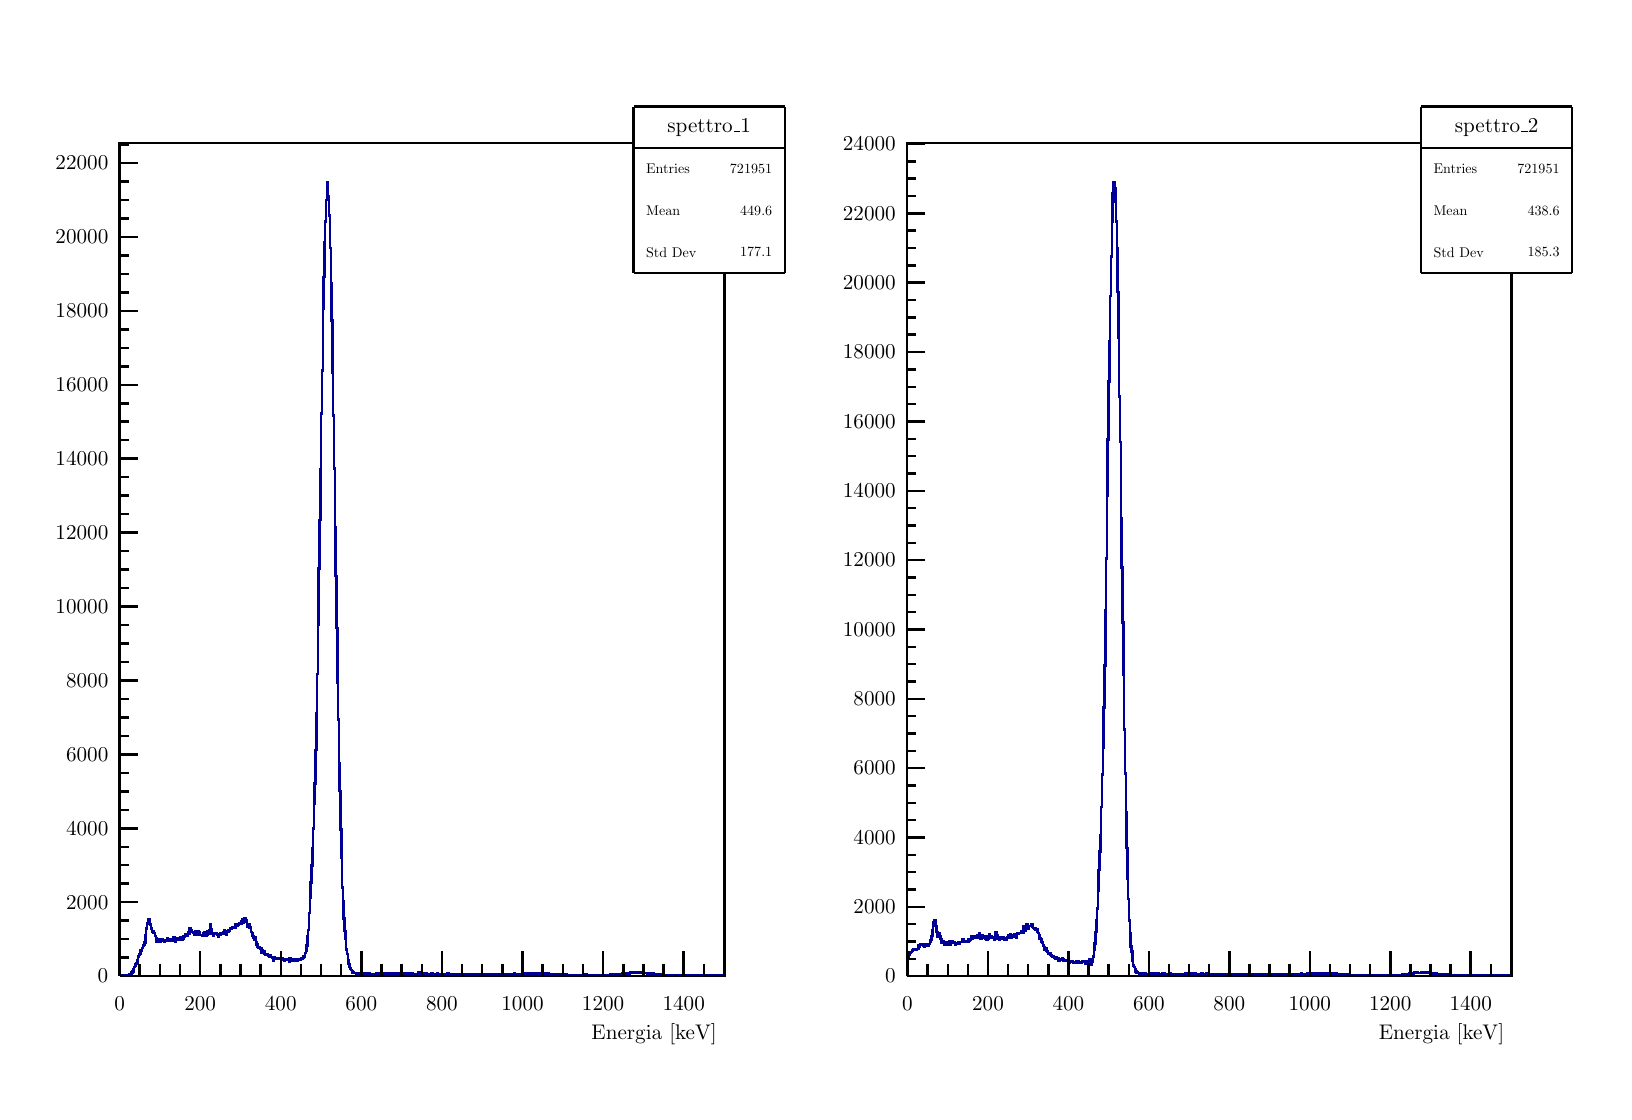
\begin{tikzpicture}
\pgfdeclareplotmark{cross} {
\pgfpathmoveto{\pgfpoint{-0.3\pgfplotmarksize}{\pgfplotmarksize}}
\pgfpathlineto{\pgfpoint{+0.3\pgfplotmarksize}{\pgfplotmarksize}}
\pgfpathlineto{\pgfpoint{+0.3\pgfplotmarksize}{0.3\pgfplotmarksize}}
\pgfpathlineto{\pgfpoint{+1\pgfplotmarksize}{0.3\pgfplotmarksize}}
\pgfpathlineto{\pgfpoint{+1\pgfplotmarksize}{-0.3\pgfplotmarksize}}
\pgfpathlineto{\pgfpoint{+0.3\pgfplotmarksize}{-0.3\pgfplotmarksize}}
\pgfpathlineto{\pgfpoint{+0.3\pgfplotmarksize}{-1.\pgfplotmarksize}}
\pgfpathlineto{\pgfpoint{-0.3\pgfplotmarksize}{-1.\pgfplotmarksize}}
\pgfpathlineto{\pgfpoint{-0.3\pgfplotmarksize}{-0.3\pgfplotmarksize}}
\pgfpathlineto{\pgfpoint{-1.\pgfplotmarksize}{-0.3\pgfplotmarksize}}
\pgfpathlineto{\pgfpoint{-1.\pgfplotmarksize}{0.3\pgfplotmarksize}}
\pgfpathlineto{\pgfpoint{-0.3\pgfplotmarksize}{0.3\pgfplotmarksize}}
\pgfpathclose
\pgfusepathqstroke
}
\pgfdeclareplotmark{cross*} {
\pgfpathmoveto{\pgfpoint{-0.3\pgfplotmarksize}{\pgfplotmarksize}}
\pgfpathlineto{\pgfpoint{+0.3\pgfplotmarksize}{\pgfplotmarksize}}
\pgfpathlineto{\pgfpoint{+0.3\pgfplotmarksize}{0.3\pgfplotmarksize}}
\pgfpathlineto{\pgfpoint{+1\pgfplotmarksize}{0.3\pgfplotmarksize}}
\pgfpathlineto{\pgfpoint{+1\pgfplotmarksize}{-0.3\pgfplotmarksize}}
\pgfpathlineto{\pgfpoint{+0.3\pgfplotmarksize}{-0.3\pgfplotmarksize}}
\pgfpathlineto{\pgfpoint{+0.3\pgfplotmarksize}{-1.\pgfplotmarksize}}
\pgfpathlineto{\pgfpoint{-0.3\pgfplotmarksize}{-1.\pgfplotmarksize}}
\pgfpathlineto{\pgfpoint{-0.3\pgfplotmarksize}{-0.3\pgfplotmarksize}}
\pgfpathlineto{\pgfpoint{-1.\pgfplotmarksize}{-0.3\pgfplotmarksize}}
\pgfpathlineto{\pgfpoint{-1.\pgfplotmarksize}{0.3\pgfplotmarksize}}
\pgfpathlineto{\pgfpoint{-0.3\pgfplotmarksize}{0.3\pgfplotmarksize}}
\pgfpathclose
\pgfusepathqfillstroke
}
\pgfdeclareplotmark{newstar} {
\pgfpathmoveto{\pgfqpoint{0pt}{\pgfplotmarksize}}
\pgfpathlineto{\pgfqpointpolar{44}{0.5\pgfplotmarksize}}
\pgfpathlineto{\pgfqpointpolar{18}{\pgfplotmarksize}}
\pgfpathlineto{\pgfqpointpolar{-20}{0.5\pgfplotmarksize}}
\pgfpathlineto{\pgfqpointpolar{-54}{\pgfplotmarksize}}
\pgfpathlineto{\pgfqpointpolar{-90}{0.5\pgfplotmarksize}}
\pgfpathlineto{\pgfqpointpolar{234}{\pgfplotmarksize}}
\pgfpathlineto{\pgfqpointpolar{198}{0.5\pgfplotmarksize}}
\pgfpathlineto{\pgfqpointpolar{162}{\pgfplotmarksize}}
\pgfpathlineto{\pgfqpointpolar{134}{0.5\pgfplotmarksize}}
\pgfpathclose
\pgfusepathqstroke
}
\pgfdeclareplotmark{newstar*} {
\pgfpathmoveto{\pgfqpoint{0pt}{\pgfplotmarksize}}
\pgfpathlineto{\pgfqpointpolar{44}{0.5\pgfplotmarksize}}
\pgfpathlineto{\pgfqpointpolar{18}{\pgfplotmarksize}}
\pgfpathlineto{\pgfqpointpolar{-20}{0.5\pgfplotmarksize}}
\pgfpathlineto{\pgfqpointpolar{-54}{\pgfplotmarksize}}
\pgfpathlineto{\pgfqpointpolar{-90}{0.5\pgfplotmarksize}}
\pgfpathlineto{\pgfqpointpolar{234}{\pgfplotmarksize}}
\pgfpathlineto{\pgfqpointpolar{198}{0.5\pgfplotmarksize}}
\pgfpathlineto{\pgfqpointpolar{162}{\pgfplotmarksize}}
\pgfpathlineto{\pgfqpointpolar{134}{0.5\pgfplotmarksize}}
\pgfpathclose
\pgfusepathqfillstroke
}
\definecolor{c}{rgb}{1,1,1};
\draw [color=c, fill=c] (0,0) rectangle (20,13.4957);
\draw [color=c, fill=c] (0.2,0.134957) rectangle (9.8,13.3607);
\draw [color=c, fill=c] (1.16,1.45754) rectangle (8.84,12.0382);
\definecolor{c}{rgb}{0,0,0};
\draw [c,line width=0.9] (1.16,1.45754) -- (1.16,12.0382) -- (8.84,12.0382) -- (8.84,1.45754) -- (1.16,1.45754);
\definecolor{c}{rgb}{1,1,1};
\draw [color=c, fill=c] (1.16,1.45754) rectangle (8.84,12.0382);
\definecolor{c}{rgb}{0,0,0};
\draw [c,line width=0.9] (1.16,1.45754) -- (1.16,12.0382) -- (8.84,12.0382) -- (8.84,1.45754) -- (1.16,1.45754);
\definecolor{c}{rgb}{0,0,0.6};
\draw [c,line width=0.9] (1.16,1.47162) -- (1.17024,1.47162) -- (1.17024,1.47209) -- (1.18048,1.47209) -- (1.18048,1.46786) -- (1.19072,1.46786) -- (1.19072,1.47209) -- (1.20096,1.47209) -- (1.20096,1.47349) -- (1.2112,1.47349) -- (1.2112,1.46927) --
 (1.22144,1.46927) -- (1.22144,1.46739) -- (1.23168,1.46739) -- (1.23168,1.47396) -- (1.24192,1.47396) -- (1.24192,1.4688) -- (1.25216,1.4688) -- (1.25216,1.47021) -- (1.2624,1.47021) -- (1.2624,1.47396) -- (1.27264,1.47396) -- (1.27264,1.47349) --
 (1.28288,1.47349) -- (1.28288,1.47819) -- (1.29312,1.47819) -- (1.29312,1.48617) -- (1.30336,1.48617) -- (1.30336,1.49227) -- (1.3136,1.49227) -- (1.3136,1.50635) -- (1.32384,1.50635) -- (1.32384,1.51621) -- (1.33408,1.51621) -- (1.33408,1.55047) --
 (1.34432,1.55047) -- (1.34432,1.57159) -- (1.35456,1.57159) -- (1.35456,1.58567) -- (1.3648,1.58567) -- (1.3648,1.60914) -- (1.37504,1.60914) -- (1.37504,1.62134) -- (1.38528,1.62134) -- (1.38528,1.6603) -- (1.39552,1.6603) -- (1.39552,1.70818) --
 (1.40576,1.70818) -- (1.40576,1.72414) -- (1.416,1.72414) -- (1.416,1.74103) -- (1.42624,1.74103) -- (1.42624,1.78515) -- (1.43648,1.78515) -- (1.43648,1.78515) -- (1.44672,1.78515) -- (1.44672,1.8166) -- (1.45696,1.8166) -- (1.45696,1.84382) --
 (1.4672,1.84382) -- (1.4672,1.85509) -- (1.47744,1.85509) -- (1.47744,1.88325) -- (1.48768,1.88325) -- (1.48768,1.97994) -- (1.49792,1.97994) -- (1.49792,2.06114) -- (1.50816,2.06114) -- (1.50816,2.12263) -- (1.5184,2.12263) -- (1.5184,2.18552) --
 (1.52864,2.18552) -- (1.52864,2.17895) -- (1.53888,2.17895) -- (1.53888,2.16252) -- (1.54912,2.16252) -- (1.54912,2.11136) -- (1.55936,2.11136) -- (1.55936,2.06302) -- (1.5696,2.06302) -- (1.5696,2.02641) -- (1.57984,2.02641) -- (1.57984,2.02734) --
 (1.59008,2.02734) -- (1.59008,2.00669) -- (1.60032,2.00669) -- (1.60032,2.00669) -- (1.61056,2.00669) -- (1.61056,1.9668) -- (1.6208,1.9668) -- (1.6208,1.9438) -- (1.63104,1.9438) -- (1.63104,1.89921) -- (1.64128,1.89921) -- (1.64128,1.92033) --
 (1.65152,1.92033) -- (1.65152,1.9086) -- (1.66176,1.9086) -- (1.66176,1.91235) -- (1.672,1.91235) -- (1.672,1.89639) -- (1.68224,1.89639) -- (1.68224,1.92549) -- (1.69248,1.92549) -- (1.69248,1.9269) -- (1.70272,1.9269) -- (1.70272,1.90766) --
 (1.71296,1.90766) -- (1.71296,1.91047) -- (1.7232,1.91047) -- (1.7232,1.88888) -- (1.73344,1.88888) -- (1.73344,1.90766) -- (1.74368,1.90766) -- (1.74368,1.91892) -- (1.75392,1.91892) -- (1.75392,1.91188) -- (1.76416,1.91188) -- (1.76416,1.93441) --
 (1.7744,1.93441) -- (1.7744,1.93206) -- (1.78464,1.93206) -- (1.78464,1.92033) -- (1.79488,1.92033) -- (1.79488,1.91) -- (1.80512,1.91) -- (1.80512,1.92268) -- (1.81536,1.92268) -- (1.81536,1.92878) -- (1.8256,1.92878) -- (1.8256,1.91188) --
 (1.83584,1.91188) -- (1.83584,1.90202) -- (1.84608,1.90202) -- (1.84608,1.94521) -- (1.85632,1.94521) -- (1.85632,1.91657) -- (1.86656,1.91657) -- (1.86656,1.89921) -- (1.8768,1.89921) -- (1.8768,1.93676) -- (1.88704,1.93676) -- (1.88704,1.93347) --
 (1.89728,1.93347) -- (1.89728,1.91939) -- (1.90752,1.91939) -- (1.90752,1.91986) -- (1.91776,1.91986) -- (1.91776,1.93723) -- (1.928,1.93723) -- (1.928,1.95459) -- (1.93824,1.95459) -- (1.93824,1.94568) -- (1.94848,1.94568) -- (1.94848,1.91423) --
 (1.95872,1.91423) -- (1.95872,1.93159) -- (1.96896,1.93159) -- (1.96896,1.97008) -- (1.9792,1.97008) -- (1.9792,1.95553) -- (1.98944,1.95553) -- (1.98944,1.97384) -- (1.99968,1.97384) -- (1.99968,1.98604) -- (2.00992,1.98604) -- (2.00992,1.98041) --
 (2.02016,1.98041) -- (2.02016,1.97525) -- (2.0304,1.97525) -- (2.0304,2.01467) -- (2.04064,2.01467) -- (2.04064,1.99543) -- (2.05088,1.99543) -- (2.05088,2.06161) -- (2.06112,2.06161) -- (2.06112,2.03016) -- (2.07136,2.03016) -- (2.07136,2.0433) --
 (2.0816,2.0433) -- (2.0816,2.01796) -- (2.09184,2.01796) -- (2.09184,2.00294) -- (2.10208,2.00294) -- (2.10208,2.00716) -- (2.11232,2.00716) -- (2.11232,1.98088) -- (2.12256,1.98088) -- (2.12256,2.02265) -- (2.1328,2.02265) -- (2.1328,2.00106) --
 (2.14304,2.00106) -- (2.14304,1.98416) -- (2.15328,1.98416) -- (2.15328,2.02453) -- (2.16352,2.02453) -- (2.16352,1.98698) -- (2.17376,1.98698) -- (2.17376,2.01279) -- (2.184,2.01279) -- (2.184,1.98135) -- (2.19424,1.98135) -- (2.19424,1.979) --
 (2.20448,1.979) -- (2.20448,1.98041) -- (2.21472,1.98041) -- (2.21472,1.96961) -- (2.22496,1.96961) -- (2.22496,1.99684) -- (2.2352,1.99684) -- (2.2352,2.01186) -- (2.24544,2.01186) -- (2.24544,1.98651) -- (2.25568,1.98651) -- (2.25568,1.96398) --
 (2.26592,1.96398) -- (2.26592,1.98651) -- (2.27616,1.98651) -- (2.27616,2.03016) -- (2.2864,2.03016) -- (2.2864,1.99731) -- (2.29664,1.99731) -- (2.29664,2.03532) -- (2.30688,2.03532) -- (2.30688,2.1123) -- (2.31712,2.1123) -- (2.31712,2.04706) --
 (2.32736,2.04706) -- (2.32736,1.9959) -- (2.3376,1.9959) -- (2.3376,2.00388) -- (2.34784,2.00388) -- (2.34784,1.97571) -- (2.35808,1.97571) -- (2.35808,2.00669) -- (2.36832,2.00669) -- (2.36832,2.00482) -- (2.37856,2.00482) -- (2.37856,1.99402) --
 (2.3888,1.99402) -- (2.3888,2.00294) -- (2.39904,2.00294) -- (2.39904,1.97806) -- (2.40928,1.97806) -- (2.40928,1.96351) -- (2.41952,1.96351) -- (2.41952,1.98604) -- (2.42976,1.98604) -- (2.42976,1.97806) -- (2.44,1.97806) -- (2.44,2.00012) --
 (2.45024,2.00012) -- (2.45024,1.9912) -- (2.46048,1.9912) -- (2.46048,1.99308) -- (2.47072,1.99308) -- (2.47072,2.01139) -- (2.48096,2.01139) -- (2.48096,2.00153) -- (2.4912,2.00153) -- (2.4912,2.03767) -- (2.50144,2.03767) -- (2.50144,2.025) --
 (2.51168,2.025) -- (2.51168,1.98463) -- (2.52192,1.98463) -- (2.52192,2.02265) -- (2.53216,2.02265) -- (2.53216,2.01937) -- (2.5424,2.01937) -- (2.5424,2.03861) -- (2.55264,2.03861) -- (2.55264,2.03157) -- (2.56288,2.03157) -- (2.56288,2.06818) --
 (2.57312,2.06818) -- (2.57312,2.06396) -- (2.58336,2.06396) -- (2.58336,2.06724) -- (2.5936,2.06724) -- (2.5936,2.07381) -- (2.60384,2.07381) -- (2.60384,2.07428) -- (2.61408,2.07428) -- (2.61408,2.06912) -- (2.62432,2.06912) -- (2.62432,2.07663) --
 (2.63456,2.07663) -- (2.63456,2.12216) -- (2.6448,2.12216) -- (2.6448,2.11699) -- (2.65504,2.11699) -- (2.65504,2.09963) -- (2.66528,2.09963) -- (2.66528,2.11324) -- (2.67552,2.11324) -- (2.67552,2.1292) -- (2.68576,2.1292) -- (2.68576,2.13483) --
 (2.696,2.13483) -- (2.696,2.12075) -- (2.70624,2.12075) -- (2.70624,2.1522) -- (2.71648,2.1522) -- (2.71648,2.17379) -- (2.72672,2.17379) -- (2.72672,2.13905) -- (2.73696,2.13905) -- (2.73696,2.14891) -- (2.7472,2.14891) -- (2.7472,2.19585) --
 (2.75744,2.19585) -- (2.75744,2.17801) -- (2.76768,2.17801) -- (2.76768,2.16346) -- (2.77792,2.16346) -- (2.77792,2.08555) -- (2.78816,2.08555) -- (2.78816,2.09071) -- (2.7984,2.09071) -- (2.7984,2.11605) -- (2.80864,2.11605) -- (2.80864,2.07334) --
 (2.81888,2.07334) -- (2.81888,2.07569) -- (2.82912,2.07569) -- (2.82912,2.01702) -- (2.83936,2.01702) -- (2.83936,2.00388) -- (2.8496,2.00388) -- (2.8496,1.96867) -- (2.85984,1.96867) -- (2.85984,1.95084) -- (2.87008,1.95084) -- (2.87008,1.91986) --
 (2.88032,1.91986) -- (2.88032,1.94849) -- (2.89056,1.94849) -- (2.89056,1.88137) -- (2.9008,1.88137) -- (2.9008,1.85931) -- (2.91104,1.85931) -- (2.91104,1.83444) -- (2.92128,1.83444) -- (2.92128,1.81425) -- (2.93152,1.81425) -- (2.93152,1.83021) --
 (2.94176,1.83021) -- (2.94176,1.80158) -- (2.952,1.80158) -- (2.952,1.80627) -- (2.96224,1.80627) -- (2.96224,1.75887) -- (2.97248,1.75887) -- (2.97248,1.78985) -- (2.98272,1.78985) -- (2.98272,1.75136) -- (2.99296,1.75136) -- (2.99296,1.76732) --
 (3.0032,1.76732) -- (3.0032,1.7415) -- (3.01344,1.7415) -- (3.01344,1.73352) -- (3.02368,1.73352) -- (3.02368,1.73728) -- (3.03392,1.73728) -- (3.03392,1.72977) -- (3.04416,1.72977) -- (3.04416,1.71756) -- (3.0544,1.71756) -- (3.0544,1.71193) --
 (3.06464,1.71193) -- (3.06464,1.7063) -- (3.07488,1.7063) -- (3.07488,1.71803) -- (3.08512,1.71803) -- (3.08512,1.69785) -- (3.09536,1.69785) -- (3.09536,1.6941) -- (3.1056,1.6941) -- (3.1056,1.65608) -- (3.11584,1.65608) -- (3.11584,1.6941) --
 (3.12608,1.6941) -- (3.12608,1.69316) -- (3.13632,1.69316) -- (3.13632,1.6833) -- (3.14656,1.6833) -- (3.14656,1.68001) -- (3.1568,1.68001) -- (3.1568,1.6833) -- (3.16704,1.6833) -- (3.16704,1.68893) -- (3.17728,1.68893) -- (3.17728,1.67955) --
 (3.18752,1.67955) -- (3.18752,1.69034) -- (3.19776,1.69034) -- (3.19776,1.67297) -- (3.208,1.67297) -- (3.208,1.66875) -- (3.21824,1.66875) -- (3.21824,1.665) -- (3.22848,1.665) -- (3.22848,1.68471) -- (3.23872,1.68471) -- (3.23872,1.66546) --
 (3.24896,1.66546) -- (3.24896,1.65842) -- (3.2592,1.65842) -- (3.2592,1.66359) -- (3.26944,1.66359) -- (3.26944,1.66218) -- (3.27968,1.66218) -- (3.27968,1.67673) -- (3.28992,1.67673) -- (3.28992,1.6772) -- (3.30016,1.6772) -- (3.30016,1.6772) --
 (3.3104,1.6772) -- (3.3104,1.64293) -- (3.32064,1.64293) -- (3.32064,1.67908) -- (3.33088,1.67908) -- (3.33088,1.67579) -- (3.34112,1.67579) -- (3.34112,1.66922) -- (3.35136,1.66922) -- (3.35136,1.64998) -- (3.3616,1.64998) -- (3.3616,1.66875) --
 (3.37184,1.66875) -- (3.37184,1.66922) -- (3.38208,1.66922) -- (3.38208,1.65373) -- (3.39232,1.65373) -- (3.39232,1.65608) -- (3.40256,1.65608) -- (3.40256,1.67438) -- (3.4128,1.67438) -- (3.4128,1.65373) -- (3.42304,1.65373) -- (3.42304,1.66969) --
 (3.43328,1.66969) -- (3.43328,1.66124) -- (3.44352,1.66124) -- (3.44352,1.665) -- (3.45376,1.665) -- (3.45376,1.67157) -- (3.464,1.67157) -- (3.464,1.67908) -- (3.47424,1.67908) -- (3.47424,1.6833) -- (3.48448,1.6833) -- (3.48448,1.68612) --
 (3.49472,1.68612) -- (3.49472,1.71616) -- (3.50496,1.71616) -- (3.50496,1.70114) -- (3.5152,1.70114) -- (3.5152,1.75183) -- (3.52544,1.75183) -- (3.52544,1.78515) -- (3.53568,1.78515) -- (3.53568,1.84523) -- (3.54592,1.84523) -- (3.54592,1.9621) --
 (3.55616,1.9621) -- (3.55616,2.04002) -- (3.5664,2.04002) -- (3.5664,2.25827) -- (3.57664,2.25827) -- (3.57664,2.44743) -- (3.58688,2.44743) -- (3.58688,2.64362) -- (3.59712,2.64362) -- (3.59712,2.86094) -- (3.60736,2.86094) -- (3.60736,3.07637) --
 (3.6176,3.07637) -- (3.6176,3.33453) -- (3.62784,3.33453) -- (3.62784,3.64853) -- (3.63808,3.64853) -- (3.63808,3.90574) -- (3.64832,3.90574) -- (3.64832,4.32911) -- (3.65856,4.32911) -- (3.65856,4.79378) -- (3.6688,4.79378) -- (3.6688,5.29365) --
 (3.67904,5.29365) -- (3.67904,5.91415) -- (3.68928,5.91415) -- (3.68928,6.63134) -- (3.69952,6.63134) -- (3.69952,7.2495) -- (3.70976,7.2495) -- (3.70976,7.89487) -- (3.72,7.89487) -- (3.72,8.60314) -- (3.73024,8.60314) -- (3.73024,9.1462) --
 (3.74048,9.1462) -- (3.74048,9.92675) -- (3.75072,9.92675) -- (3.75072,10.3337) -- (3.76096,10.3337) -- (3.76096,10.7829) -- (3.7712,10.7829) -- (3.7712,11.041) -- (3.78144,11.041) -- (3.78144,11.3133) -- (3.79168,11.3133) -- (3.79168,11.5343) --
 (3.80192,11.5343) -- (3.80192,11.3372) -- (3.81216,11.3372) -- (3.81216,11.356) -- (3.8224,11.356) -- (3.8224,11.1152) -- (3.83264,11.1152) -- (3.83264,10.7059) -- (3.84288,10.7059) -- (3.84288,10.2506) -- (3.85312,10.2506) -- (3.85312,9.78172) --
 (3.86336,9.78172) -- (3.86336,9.11616) -- (3.8736,9.11616) -- (3.8736,8.5778) -- (3.88384,8.5778) -- (3.88384,7.90285) -- (3.89408,7.90285) -- (3.89408,7.15375) -- (3.90432,7.15375) -- (3.90432,6.53982) -- (3.91456,6.53982) -- (3.91456,5.8766) --
 (3.9248,5.8766) -- (3.9248,5.18758) -- (3.93504,5.18758) -- (3.93504,4.71399) -- (3.94528,4.71399) -- (3.94528,4.15591) -- (3.95552,4.15591) -- (3.95552,3.80999) -- (3.96576,3.80999) -- (3.96576,3.31857) -- (3.976,3.31857) -- (3.976,2.96044) --
 (3.98624,2.96044) -- (3.98624,2.58401) -- (3.99648,2.58401) -- (3.99648,2.41316) -- (4.00672,2.41316) -- (4.00672,2.19209) -- (4.01696,2.19209) -- (4.01696,2.03345) -- (4.0272,2.03345) -- (4.0272,1.93676) -- (4.03744,1.93676) -- (4.03744,1.79313) --
 (4.04768,1.79313) -- (4.04768,1.73681) -- (4.05792,1.73681) -- (4.05792,1.665) -- (4.06816,1.665) -- (4.06816,1.60961) -- (4.0784,1.60961) -- (4.0784,1.57441) -- (4.08864,1.57441) -- (4.08864,1.55329) -- (4.09888,1.55329) -- (4.09888,1.53686) --
 (4.10912,1.53686) -- (4.10912,1.52372) -- (4.11936,1.52372) -- (4.11936,1.50588) -- (4.1296,1.50588) -- (4.1296,1.50823) -- (4.13984,1.50823) -- (4.13984,1.49602) -- (4.15008,1.49602) -- (4.15008,1.4979) -- (4.16032,1.4979) -- (4.16032,1.49321) --
 (4.17056,1.49321) -- (4.17056,1.49462) -- (4.1808,1.49462) -- (4.1808,1.48476) -- (4.19104,1.48476) -- (4.19104,1.48664) -- (4.20128,1.48664) -- (4.20128,1.49555) -- (4.21152,1.49555) -- (4.21152,1.49837) -- (4.22176,1.49837) -- (4.22176,1.49462) --
 (4.232,1.49462) -- (4.232,1.48945) -- (4.24224,1.48945) -- (4.24224,1.49274) -- (4.25248,1.49274) -- (4.25248,1.49649) -- (4.26272,1.49649) -- (4.26272,1.48851) -- (4.27296,1.48851) -- (4.27296,1.49509) -- (4.2832,1.49509) -- (4.2832,1.48898) --
 (4.29344,1.48898) -- (4.29344,1.4857) -- (4.30368,1.4857) -- (4.30368,1.49039) -- (4.31392,1.49039) -- (4.31392,1.49602) -- (4.32416,1.49602) -- (4.32416,1.49039) -- (4.3344,1.49039) -- (4.3344,1.4857) -- (4.34464,1.4857) -- (4.34464,1.48429) --
 (4.35488,1.48429) -- (4.35488,1.48664) -- (4.36512,1.48664) -- (4.36512,1.48711) -- (4.37536,1.48711) -- (4.37536,1.48288) -- (4.3856,1.48288) -- (4.3856,1.48382) -- (4.39584,1.48382) -- (4.39584,1.48382) -- (4.40608,1.48382) -- (4.40608,1.48194) --
 (4.41632,1.48194) -- (4.41632,1.48898) -- (4.42656,1.48898) -- (4.42656,1.48335) -- (4.4368,1.48335) -- (4.4368,1.48288) -- (4.44704,1.48288) -- (4.44704,1.48053) -- (4.45728,1.48053) -- (4.45728,1.48992) -- (4.46752,1.48992) -- (4.46752,1.48664) --
 (4.47776,1.48664) -- (4.47776,1.49321) -- (4.488,1.49321) -- (4.488,1.49133) -- (4.49824,1.49133) -- (4.49824,1.48523) -- (4.50848,1.48523) -- (4.50848,1.49039) -- (4.51872,1.49039) -- (4.51872,1.48523) -- (4.52896,1.48523) -- (4.52896,1.48429) --
 (4.5392,1.48429) -- (4.5392,1.48804) -- (4.54944,1.48804) -- (4.54944,1.48992) -- (4.55968,1.48992) -- (4.55968,1.48945) -- (4.56992,1.48945) -- (4.56992,1.48898) -- (4.58016,1.48898) -- (4.58016,1.48898) -- (4.5904,1.48898) -- (4.5904,1.48898) --
 (4.60064,1.48898) -- (4.60064,1.48851) -- (4.61088,1.48851) -- (4.61088,1.49415) -- (4.62112,1.49415) -- (4.62112,1.48664) -- (4.63136,1.48664) -- (4.63136,1.48382) -- (4.6416,1.48382) -- (4.6416,1.48007) -- (4.65184,1.48007) -- (4.65184,1.49227) --
 (4.66208,1.49227) -- (4.66208,1.48664) -- (4.67232,1.48664) -- (4.67232,1.48617) -- (4.68256,1.48617) -- (4.68256,1.48335) -- (4.6928,1.48335) -- (4.6928,1.48945) -- (4.70304,1.48945) -- (4.70304,1.49368) -- (4.71328,1.49368) -- (4.71328,1.48523) --
 (4.72352,1.48523) -- (4.72352,1.49321) -- (4.73376,1.49321) -- (4.73376,1.48758) -- (4.744,1.48758) -- (4.744,1.49274) -- (4.75424,1.49274) -- (4.75424,1.48382) -- (4.76448,1.48382) -- (4.76448,1.48523) -- (4.77472,1.48523) -- (4.77472,1.49039) --
 (4.78496,1.49039) -- (4.78496,1.48898) -- (4.7952,1.48898) -- (4.7952,1.49039) -- (4.80544,1.49039) -- (4.80544,1.48851) -- (4.81568,1.48851) -- (4.81568,1.49696) -- (4.82592,1.49696) -- (4.82592,1.49696) -- (4.83616,1.49696) -- (4.83616,1.48758) --
 (4.8464,1.48758) -- (4.8464,1.48992) -- (4.85664,1.48992) -- (4.85664,1.48758) -- (4.86688,1.48758) -- (4.86688,1.47866) -- (4.87712,1.47866) -- (4.87712,1.49462) -- (4.88736,1.49462) -- (4.88736,1.48758) -- (4.8976,1.48758) -- (4.8976,1.48523) --
 (4.90784,1.48523) -- (4.90784,1.48476) -- (4.91808,1.48476) -- (4.91808,1.48711) -- (4.92832,1.48711) -- (4.92832,1.48382) -- (4.93856,1.48382) -- (4.93856,1.48523) -- (4.9488,1.48523) -- (4.9488,1.49415) -- (4.95904,1.49415) -- (4.95904,1.50072) --
 (4.96928,1.50072) -- (4.96928,1.481) -- (4.97952,1.481) -- (4.97952,1.4918) -- (4.98976,1.4918) -- (4.98976,1.48476) -- (5,1.48476) -- (5,1.4796) -- (5.01024,1.4796) -- (5.01024,1.48194) -- (5.02048,1.48194) -- (5.02048,1.48992) -- (5.03072,1.48992)
 -- (5.03072,1.481) -- (5.04096,1.481) -- (5.04096,1.48335) -- (5.0512,1.48335) -- (5.0512,1.49227) -- (5.06144,1.49227) -- (5.06144,1.48382) -- (5.07168,1.48382) -- (5.07168,1.48288) -- (5.08192,1.48288) -- (5.08192,1.48194) -- (5.09216,1.48194) --
 (5.09216,1.48523) -- (5.1024,1.48523) -- (5.1024,1.48288) -- (5.11264,1.48288) -- (5.11264,1.47819) -- (5.12288,1.47819) -- (5.12288,1.48804) -- (5.13312,1.48804) -- (5.13312,1.48804) -- (5.14336,1.48804) -- (5.14336,1.48664) -- (5.1536,1.48664) --
 (5.1536,1.48711) -- (5.16384,1.48711) -- (5.16384,1.481) -- (5.17408,1.481) -- (5.17408,1.48288) -- (5.18432,1.48288) -- (5.18432,1.48288) -- (5.19456,1.48288) -- (5.19456,1.48945) -- (5.2048,1.48945) -- (5.2048,1.48476) -- (5.21504,1.48476) --
 (5.21504,1.48758) -- (5.22528,1.48758) -- (5.22528,1.4796) -- (5.23552,1.4796) -- (5.23552,1.48758) -- (5.24576,1.48758) -- (5.24576,1.48711) -- (5.256,1.48711) -- (5.256,1.48523) -- (5.26624,1.48523) -- (5.26624,1.48429) -- (5.27648,1.48429) --
 (5.27648,1.48241) -- (5.28672,1.48241) -- (5.28672,1.481) -- (5.29696,1.481) -- (5.29696,1.48711) -- (5.3072,1.48711) -- (5.3072,1.48476) -- (5.31744,1.48476) -- (5.31744,1.48007) -- (5.32768,1.48007) -- (5.32768,1.48804) -- (5.33792,1.48804) --
 (5.33792,1.48664) -- (5.34816,1.48664) -- (5.34816,1.4796) -- (5.3584,1.4796) -- (5.3584,1.48664) -- (5.36864,1.48664) -- (5.36864,1.47584) -- (5.37888,1.47584) -- (5.37888,1.47725) -- (5.38912,1.47725) -- (5.38912,1.47866) -- (5.39936,1.47866) --
 (5.39936,1.4857) -- (5.4096,1.4857) -- (5.4096,1.47772) -- (5.41984,1.47772) -- (5.41984,1.48288) -- (5.43008,1.48288) -- (5.43008,1.4796) -- (5.44032,1.4796) -- (5.44032,1.48523) -- (5.45056,1.48523) -- (5.45056,1.48476) -- (5.4608,1.48476) --
 (5.4608,1.48147) -- (5.47104,1.48147) -- (5.47104,1.47819) -- (5.48128,1.47819) -- (5.48128,1.47913) -- (5.49152,1.47913) -- (5.49152,1.48429) -- (5.50176,1.48429) -- (5.50176,1.48194) -- (5.512,1.48194) -- (5.512,1.47819) -- (5.52224,1.47819) --
 (5.52224,1.48194) -- (5.53248,1.48194) -- (5.53248,1.4796) -- (5.54272,1.4796) -- (5.54272,1.47725) -- (5.55296,1.47725) -- (5.55296,1.4796) -- (5.5632,1.4796) -- (5.5632,1.47678) -- (5.57344,1.47678) -- (5.57344,1.48288) -- (5.58368,1.48288) --
 (5.58368,1.47772) -- (5.59392,1.47772) -- (5.59392,1.47584) -- (5.60416,1.47584) -- (5.60416,1.47725) -- (5.6144,1.47725) -- (5.6144,1.47772) -- (5.62464,1.47772) -- (5.62464,1.4796) -- (5.63488,1.4796) -- (5.63488,1.4749) -- (5.64512,1.4749) --
 (5.64512,1.47913) -- (5.65536,1.47913) -- (5.65536,1.47725) -- (5.6656,1.47725) -- (5.6656,1.47772) -- (5.67584,1.47772) -- (5.67584,1.48007) -- (5.68608,1.48007) -- (5.68608,1.481) -- (5.69632,1.481) -- (5.69632,1.47913) -- (5.70656,1.47913) --
 (5.70656,1.47302) -- (5.7168,1.47302) -- (5.7168,1.481) -- (5.72704,1.481) -- (5.72704,1.4796) -- (5.73728,1.4796) -- (5.73728,1.48523) -- (5.74752,1.48523) -- (5.74752,1.47866) -- (5.75776,1.47866) -- (5.75776,1.47349) -- (5.768,1.47349) --
 (5.768,1.47725) -- (5.77824,1.47725) -- (5.77824,1.48382) -- (5.78848,1.48382) -- (5.78848,1.48147) -- (5.79872,1.48147) -- (5.79872,1.48007) -- (5.80896,1.48007) -- (5.80896,1.47913) -- (5.8192,1.47913) -- (5.8192,1.4796) -- (5.82944,1.4796) --
 (5.82944,1.481) -- (5.83968,1.481) -- (5.83968,1.47537) -- (5.84992,1.47537) -- (5.84992,1.48147) -- (5.86016,1.48147) -- (5.86016,1.48147) -- (5.8704,1.48147) -- (5.8704,1.48241) -- (5.88064,1.48241) -- (5.88064,1.47725) -- (5.89088,1.47725) --
 (5.89088,1.47725) -- (5.90112,1.47725) -- (5.90112,1.47725) -- (5.91136,1.47725) -- (5.91136,1.48147) -- (5.9216,1.48147) -- (5.9216,1.47631) -- (5.93184,1.47631) -- (5.93184,1.47913) -- (5.94208,1.47913) -- (5.94208,1.47866) -- (5.95232,1.47866) --
 (5.95232,1.4796) -- (5.96256,1.4796) -- (5.96256,1.48617) -- (5.9728,1.48617) -- (5.9728,1.4796) -- (5.98304,1.4796) -- (5.98304,1.48053) -- (5.99328,1.48053) -- (5.99328,1.47866) -- (6.00352,1.47866) -- (6.00352,1.48007) -- (6.01376,1.48007) --
 (6.01376,1.48288) -- (6.024,1.48288) -- (6.024,1.48335) -- (6.03424,1.48335) -- (6.03424,1.47866) -- (6.04448,1.47866) -- (6.04448,1.48382) -- (6.05472,1.48382) -- (6.05472,1.47678) -- (6.06496,1.47678) -- (6.06496,1.48335) -- (6.0752,1.48335) --
 (6.0752,1.48523) -- (6.08544,1.48523) -- (6.08544,1.48194) -- (6.09568,1.48194) -- (6.09568,1.48194) -- (6.10592,1.48194) -- (6.10592,1.48288) -- (6.11616,1.48288) -- (6.11616,1.48382) -- (6.1264,1.48382) -- (6.1264,1.4857) -- (6.13664,1.4857) --
 (6.13664,1.48053) -- (6.14688,1.48053) -- (6.14688,1.48617) -- (6.15712,1.48617) -- (6.15712,1.4857) -- (6.16736,1.4857) -- (6.16736,1.48945) -- (6.1776,1.48945) -- (6.1776,1.48617) -- (6.18784,1.48617) -- (6.18784,1.48007) -- (6.19808,1.48007) --
 (6.19808,1.48429) -- (6.20832,1.48429) -- (6.20832,1.48241) -- (6.21856,1.48241) -- (6.21856,1.48523) -- (6.2288,1.48523) -- (6.2288,1.48382) -- (6.23904,1.48382) -- (6.23904,1.48523) -- (6.24928,1.48523) -- (6.24928,1.48617) -- (6.25952,1.48617) --
 (6.25952,1.48711) -- (6.26976,1.48711) -- (6.26976,1.48241) -- (6.28,1.48241) -- (6.28,1.48804) -- (6.29024,1.48804) -- (6.29024,1.48617) -- (6.30048,1.48617) -- (6.30048,1.49415) -- (6.31072,1.49415) -- (6.31072,1.49274) -- (6.32096,1.49274) --
 (6.32096,1.49368) -- (6.3312,1.49368) -- (6.3312,1.48851) -- (6.34144,1.48851) -- (6.34144,1.48992) -- (6.35168,1.48992) -- (6.35168,1.48898) -- (6.36192,1.48898) -- (6.36192,1.49086) -- (6.37216,1.49086) -- (6.37216,1.4857) -- (6.3824,1.4857) --
 (6.3824,1.48945) -- (6.39264,1.48945) -- (6.39264,1.48523) -- (6.40288,1.48523) -- (6.40288,1.49133) -- (6.41312,1.49133) -- (6.41312,1.49884) -- (6.42336,1.49884) -- (6.42336,1.49321) -- (6.4336,1.49321) -- (6.4336,1.49743) -- (6.44384,1.49743) --
 (6.44384,1.49133) -- (6.45408,1.49133) -- (6.45408,1.48711) -- (6.46432,1.48711) -- (6.46432,1.49555) -- (6.47456,1.49555) -- (6.47456,1.49227) -- (6.4848,1.49227) -- (6.4848,1.4857) -- (6.49504,1.4857) -- (6.49504,1.49086) -- (6.50528,1.49086) --
 (6.50528,1.49321) -- (6.51552,1.49321) -- (6.51552,1.49133) -- (6.52576,1.49133) -- (6.52576,1.48758) -- (6.536,1.48758) -- (6.536,1.48992) -- (6.54624,1.48992) -- (6.54624,1.48382) -- (6.55648,1.48382) -- (6.55648,1.48664) -- (6.56672,1.48664) --
 (6.56672,1.48898) -- (6.57696,1.48898) -- (6.57696,1.49133) -- (6.5872,1.49133) -- (6.5872,1.48476) -- (6.59744,1.48476) -- (6.59744,1.48992) -- (6.60768,1.48992) -- (6.60768,1.48335) -- (6.61792,1.48335) -- (6.61792,1.48429) -- (6.62816,1.48429) --
 (6.62816,1.47913) -- (6.6384,1.47913) -- (6.6384,1.48335) -- (6.64864,1.48335) -- (6.64864,1.481) -- (6.65888,1.481) -- (6.65888,1.47913) -- (6.66912,1.47913) -- (6.66912,1.47819) -- (6.67936,1.47819) -- (6.67936,1.481) -- (6.6896,1.481) --
 (6.6896,1.48053) -- (6.69984,1.48053) -- (6.69984,1.47678) -- (6.71008,1.47678) -- (6.71008,1.47725) -- (6.72032,1.47725) -- (6.72032,1.47772) -- (6.73056,1.47772) -- (6.73056,1.48194) -- (6.7408,1.48194) -- (6.7408,1.47631) -- (6.75104,1.47631) --
 (6.75104,1.47162) -- (6.76128,1.47162) -- (6.76128,1.4749) -- (6.77152,1.4749) -- (6.77152,1.47725) -- (6.78176,1.47725) -- (6.78176,1.46974) -- (6.792,1.46974) -- (6.792,1.47302) -- (6.80224,1.47302) -- (6.80224,1.47115) -- (6.81248,1.47115) --
 (6.81248,1.47302) -- (6.82272,1.47302) -- (6.82272,1.47631) -- (6.83296,1.47631) -- (6.83296,1.47068) -- (6.8432,1.47068) -- (6.8432,1.47162) -- (6.85344,1.47162) -- (6.85344,1.46927) -- (6.86368,1.46927) -- (6.86368,1.46927) -- (6.87392,1.46927) --
 (6.87392,1.47162) -- (6.88416,1.47162) -- (6.88416,1.47115) -- (6.8944,1.47115) -- (6.8944,1.47068) -- (6.90464,1.47068) -- (6.90464,1.47209) -- (6.91488,1.47209) -- (6.91488,1.47115) -- (6.92512,1.47115) -- (6.92512,1.4688) -- (6.93536,1.4688) --
 (6.93536,1.46833) -- (6.9456,1.46833) -- (6.9456,1.47115) -- (6.95584,1.47115) -- (6.95584,1.46786) -- (6.96608,1.46786) -- (6.96608,1.47162) -- (6.97632,1.47162) -- (6.97632,1.4688) -- (6.98656,1.4688) -- (6.98656,1.46645) -- (6.9968,1.46645) --
 (6.9968,1.47162) -- (7.00704,1.47162) -- (7.00704,1.47021) -- (7.01728,1.47021) -- (7.01728,1.46786) -- (7.02752,1.46786) -- (7.02752,1.46739) -- (7.03776,1.46739) -- (7.03776,1.46786) -- (7.048,1.46786) -- (7.048,1.46927) -- (7.05824,1.46927) --
 (7.05824,1.46692) -- (7.06848,1.46692) -- (7.06848,1.4749) -- (7.07872,1.4749) -- (7.07872,1.47678) -- (7.08896,1.47678) -- (7.08896,1.4749) -- (7.0992,1.4749) -- (7.0992,1.47068) -- (7.10944,1.47068) -- (7.10944,1.47021) -- (7.11968,1.47021) --
 (7.11968,1.47115) -- (7.12992,1.47115) -- (7.12992,1.46739) -- (7.14016,1.46739) -- (7.14016,1.46739) -- (7.1504,1.46739) -- (7.1504,1.46786) -- (7.16064,1.46786) -- (7.16064,1.47162) -- (7.17088,1.47162) -- (7.17088,1.4688) -- (7.18112,1.4688) --
 (7.18112,1.46974) -- (7.19136,1.46974) -- (7.19136,1.46833) -- (7.2016,1.46833) -- (7.2016,1.47021) -- (7.21184,1.47021) -- (7.21184,1.46833) -- (7.22208,1.46833) -- (7.22208,1.46692) -- (7.23232,1.46692) -- (7.23232,1.46833) -- (7.24256,1.46833) --
 (7.24256,1.46786) -- (7.2528,1.46786) -- (7.2528,1.47209) -- (7.26304,1.47209) -- (7.26304,1.46974) -- (7.27328,1.46974) -- (7.27328,1.47256) -- (7.28352,1.47256) -- (7.28352,1.46598) -- (7.29376,1.46598) -- (7.29376,1.47021) -- (7.304,1.47021) --
 (7.304,1.47021) -- (7.31424,1.47021) -- (7.31424,1.46833) -- (7.32448,1.46833) -- (7.32448,1.47443) -- (7.33472,1.47443) -- (7.33472,1.46833) -- (7.34496,1.46833) -- (7.34496,1.46974) -- (7.3552,1.46974) -- (7.3552,1.47302) -- (7.36544,1.47302) --
 (7.36544,1.47349) -- (7.37568,1.47349) -- (7.37568,1.46927) -- (7.38592,1.46927) -- (7.38592,1.47302) -- (7.39616,1.47302) -- (7.39616,1.47819) -- (7.4064,1.47819) -- (7.4064,1.47349) -- (7.41664,1.47349) -- (7.41664,1.47396) -- (7.42688,1.47396) --
 (7.42688,1.47256) -- (7.43712,1.47256) -- (7.43712,1.47396) -- (7.44736,1.47396) -- (7.44736,1.47866) -- (7.4576,1.47866) -- (7.4576,1.47678) -- (7.46784,1.47678) -- (7.46784,1.48194) -- (7.47808,1.48194) -- (7.47808,1.47631) -- (7.48832,1.47631) --
 (7.48832,1.47913) -- (7.49856,1.47913) -- (7.49856,1.48523) -- (7.5088,1.48523) -- (7.5088,1.47631) -- (7.51904,1.47631) -- (7.51904,1.47866) -- (7.52928,1.47866) -- (7.52928,1.48664) -- (7.53952,1.48664) -- (7.53952,1.48898) -- (7.54976,1.48898) --
 (7.54976,1.48898) -- (7.56,1.48898) -- (7.56,1.49368) -- (7.57024,1.49368) -- (7.57024,1.48664) -- (7.58048,1.48664) -- (7.58048,1.48758) -- (7.59072,1.48758) -- (7.59072,1.49649) -- (7.60096,1.49649) -- (7.60096,1.49509) -- (7.6112,1.49509) --
 (7.6112,1.49274) -- (7.62144,1.49274) -- (7.62144,1.49415) -- (7.63168,1.49415) -- (7.63168,1.49039) -- (7.64192,1.49039) -- (7.64192,1.504) -- (7.65216,1.504) -- (7.65216,1.50166) -- (7.6624,1.50166) -- (7.6624,1.50259) -- (7.67264,1.50259) --
 (7.67264,1.49837) -- (7.68288,1.49837) -- (7.68288,1.50025) -- (7.69312,1.50025) -- (7.69312,1.50025) -- (7.70336,1.50025) -- (7.70336,1.50964) -- (7.7136,1.50964) -- (7.7136,1.50119) -- (7.72384,1.50119) -- (7.72384,1.51104) -- (7.73408,1.51104) --
 (7.73408,1.50259) -- (7.74432,1.50259) -- (7.74432,1.50166) -- (7.75456,1.50166) -- (7.75456,1.49696) -- (7.7648,1.49696) -- (7.7648,1.50635) -- (7.77504,1.50635) -- (7.77504,1.50541) -- (7.78528,1.50541) -- (7.78528,1.50166) -- (7.79552,1.50166) --
 (7.79552,1.50119) -- (7.80576,1.50119) -- (7.80576,1.50119) -- (7.816,1.50119) -- (7.816,1.49837) -- (7.82624,1.49837) -- (7.82624,1.49509) -- (7.83648,1.49509) -- (7.83648,1.4979) -- (7.84672,1.4979) -- (7.84672,1.49649) -- (7.85696,1.49649) --
 (7.85696,1.49321) -- (7.8672,1.49321) -- (7.8672,1.49086) -- (7.87744,1.49086) -- (7.87744,1.49555) -- (7.88768,1.49555) -- (7.88768,1.48992) -- (7.89792,1.48992) -- (7.89792,1.49227) -- (7.90816,1.49227) -- (7.90816,1.48664) -- (7.9184,1.48664) --
 (7.9184,1.48194) -- (7.92864,1.48194) -- (7.92864,1.48898) -- (7.93888,1.48898) -- (7.93888,1.47725) -- (7.94912,1.47725) -- (7.94912,1.48382) -- (7.95936,1.48382) -- (7.95936,1.4796) -- (7.9696,1.4796) -- (7.9696,1.48241) -- (7.97984,1.48241) --
 (7.97984,1.47866) -- (7.99008,1.47866) -- (7.99008,1.481) -- (8.00032,1.481) -- (8.00032,1.48147) -- (8.01056,1.48147) -- (8.01056,1.48053) -- (8.0208,1.48053) -- (8.0208,1.47584) -- (8.03104,1.47584) -- (8.03104,1.47772) -- (8.04128,1.47772) --
 (8.04128,1.47349) -- (8.05152,1.47349) -- (8.05152,1.47209) -- (8.06176,1.47209) -- (8.06176,1.47349) -- (8.072,1.47349) -- (8.072,1.47162) -- (8.08224,1.47162) -- (8.08224,1.46833) -- (8.09248,1.46833) -- (8.09248,1.46739) -- (8.10272,1.46739) --
 (8.10272,1.46645) -- (8.11296,1.46645) -- (8.11296,1.47349) -- (8.1232,1.47349) -- (8.1232,1.47021) -- (8.13344,1.47021) -- (8.13344,1.46552) -- (8.14368,1.46552) -- (8.14368,1.46786) -- (8.15392,1.46786) -- (8.15392,1.46974) -- (8.16416,1.46974) --
 (8.16416,1.46598) -- (8.1744,1.46598) -- (8.1744,1.47068) -- (8.18464,1.47068) -- (8.18464,1.46786) -- (8.19488,1.46786) -- (8.19488,1.46974) -- (8.20512,1.46974) -- (8.20512,1.46645) -- (8.21536,1.46645) -- (8.21536,1.46786) -- (8.2256,1.46786) --
 (8.2256,1.46317) -- (8.23584,1.46317) -- (8.23584,1.46505) -- (8.24608,1.46505) -- (8.24608,1.47021) -- (8.25632,1.47021) -- (8.25632,1.46505) -- (8.26656,1.46505) -- (8.26656,1.46833) -- (8.2768,1.46833) -- (8.2768,1.46833) -- (8.28704,1.46833) --
 (8.28704,1.46786) -- (8.29728,1.46786) -- (8.29728,1.47021) -- (8.30752,1.47021) -- (8.30752,1.46786) -- (8.31776,1.46786) -- (8.31776,1.46692) -- (8.328,1.46692) -- (8.328,1.46458) -- (8.33824,1.46458) -- (8.33824,1.4688) -- (8.34848,1.4688) --
 (8.34848,1.47021) -- (8.35872,1.47021) -- (8.35872,1.46598) -- (8.36896,1.46598) -- (8.36896,1.46598) -- (8.3792,1.46598) -- (8.3792,1.46974) -- (8.38944,1.46974) -- (8.38944,1.4688) -- (8.39968,1.4688) -- (8.39968,1.46833) -- (8.40992,1.46833) --
 (8.40992,1.47115) -- (8.42016,1.47115) -- (8.42016,1.46692) -- (8.4304,1.46692) -- (8.4304,1.46505) -- (8.44064,1.46505) -- (8.44064,1.46786) -- (8.45088,1.46786) -- (8.45088,1.46833) -- (8.46112,1.46833) -- (8.46112,1.46927) -- (8.47136,1.46927) --
 (8.47136,1.46974) -- (8.4816,1.46974) -- (8.4816,1.46692) -- (8.49184,1.46692) -- (8.49184,1.46927) -- (8.50208,1.46927) -- (8.50208,1.46739) -- (8.51232,1.46739) -- (8.51232,1.46927) -- (8.52256,1.46927) -- (8.52256,1.46739) -- (8.5328,1.46739) --
 (8.5328,1.4688) -- (8.54304,1.4688) -- (8.54304,1.46458) -- (8.55328,1.46458) -- (8.55328,1.46505) -- (8.56352,1.46505) -- (8.56352,1.46692) -- (8.57376,1.46692) -- (8.57376,1.46364) -- (8.584,1.46364) -- (8.584,1.46598) -- (8.59424,1.46598) --
 (8.59424,1.47349) -- (8.60448,1.47349) -- (8.60448,1.4688) -- (8.61472,1.4688) -- (8.61472,1.46739) -- (8.62496,1.46739) -- (8.62496,1.46645) -- (8.6352,1.46645) -- (8.6352,1.46927) -- (8.64544,1.46927) -- (8.64544,1.46692) -- (8.65568,1.46692) --
 (8.65568,1.46505) -- (8.66592,1.46505) -- (8.66592,1.46786) -- (8.67616,1.46786) -- (8.67616,1.46974) -- (8.6864,1.46974) -- (8.6864,1.46598) -- (8.69664,1.46598) -- (8.69664,1.47068) -- (8.70688,1.47068) -- (8.70688,1.46739) -- (8.71712,1.46739) --
 (8.71712,1.46645) -- (8.72736,1.46645) -- (8.72736,1.46974) -- (8.7376,1.46974) -- (8.7376,1.4688) -- (8.74784,1.4688) -- (8.74784,1.46411) -- (8.75808,1.46411) -- (8.75808,1.46786) -- (8.76832,1.46786) -- (8.76832,1.46552) -- (8.77856,1.46552) --
 (8.77856,1.46739) -- (8.7888,1.46739) -- (8.7888,1.46552) -- (8.79904,1.46552) -- (8.79904,1.46739) -- (8.80928,1.46739) -- (8.80928,1.46552) -- (8.81952,1.46552) -- (8.81952,1.46645) -- (8.82976,1.46645) -- (8.82976,1.46552) -- (8.84,1.46552);
\definecolor{c}{rgb}{1,1,1};
\draw [color=c, fill=c] (7.688,10.3849) rectangle (9.608,12.5011);
\definecolor{c}{rgb}{0,0,0};
\draw [c,line width=0.9] (7.688,10.3849) -- (9.608,10.3849);
\draw [c,line width=0.9] (9.608,10.3849) -- (9.608,12.5011);
\draw [c,line width=0.9] (9.608,12.5011) -- (7.688,12.5011);
\draw [c,line width=0.9] (7.688,12.5011) -- (7.688,10.3849);
\draw (8.648,12.2366) node[scale=0.763748, color=c, rotate=0]{spettro\_1};
\draw [c,line width=0.9] (7.688,11.972) -- (9.608,11.972);
\draw [anchor= west] (7.784,11.7075) node[scale=0.509166, color=c, rotate=0]{Entries };
\draw [anchor= east] (9.512,11.7075) node[scale=0.509166, color=c, rotate=0]{ 721951};
\draw [anchor= west] (7.784,11.1785) node[scale=0.509166, color=c, rotate=0]{Mean  };
\draw [anchor= east] (9.512,11.1785) node[scale=0.509166, color=c, rotate=0]{  449.6};
\draw [anchor= west] (7.784,10.6495) node[scale=0.509166, color=c, rotate=0]{Std Dev   };
\draw [anchor= east] (9.512,10.6495) node[scale=0.509166, color=c, rotate=0]{  177.1};
\draw [c,line width=0.9] (1.16,1.45754) -- (8.84,1.45754);
\draw [anchor= east] (8.84,0.716892) node[scale=0.763748, color=c, rotate=0]{Energia [keV]};
\draw [c,line width=0.9] (1.16007,1.77495) -- (1.16007,1.45754);
\draw [c,line width=0.9] (1.41594,1.61625) -- (1.41594,1.45754);
\draw [c,line width=0.9] (1.67182,1.61625) -- (1.67182,1.45754);
\draw [c,line width=0.9] (1.92769,1.61625) -- (1.92769,1.45754);
\draw [c,line width=0.9] (2.18356,1.77495) -- (2.18356,1.45754);
\draw [c,line width=0.9] (2.43943,1.61625) -- (2.43943,1.45754);
\draw [c,line width=0.9] (2.6953,1.61625) -- (2.6953,1.45754);
\draw [c,line width=0.9] (2.95118,1.61625) -- (2.95118,1.45754);
\draw [c,line width=0.9] (3.20705,1.77495) -- (3.20705,1.45754);
\draw [c,line width=0.9] (3.46292,1.61625) -- (3.46292,1.45754);
\draw [c,line width=0.9] (3.71879,1.61625) -- (3.71879,1.45754);
\draw [c,line width=0.9] (3.97467,1.61625) -- (3.97467,1.45754);
\draw [c,line width=0.9] (4.23054,1.77495) -- (4.23054,1.45754);
\draw [c,line width=0.9] (4.48641,1.61625) -- (4.48641,1.45754);
\draw [c,line width=0.9] (4.74228,1.61625) -- (4.74228,1.45754);
\draw [c,line width=0.9] (4.99815,1.61625) -- (4.99815,1.45754);
\draw [c,line width=0.9] (5.25403,1.77495) -- (5.25403,1.45754);
\draw [c,line width=0.9] (5.5099,1.61625) -- (5.5099,1.45754);
\draw [c,line width=0.9] (5.76577,1.61625) -- (5.76577,1.45754);
\draw [c,line width=0.9] (6.02164,1.61625) -- (6.02164,1.45754);
\draw [c,line width=0.9] (6.27752,1.77495) -- (6.27752,1.45754);
\draw [c,line width=0.9] (6.53339,1.61625) -- (6.53339,1.45754);
\draw [c,line width=0.9] (6.78926,1.61625) -- (6.78926,1.45754);
\draw [c,line width=0.9] (7.04513,1.61625) -- (7.04513,1.45754);
\draw [c,line width=0.9] (7.301,1.77495) -- (7.301,1.45754);
\draw [c,line width=0.9] (7.55688,1.61625) -- (7.55688,1.45754);
\draw [c,line width=0.9] (7.81275,1.61625) -- (7.81275,1.45754);
\draw [c,line width=0.9] (8.06862,1.61625) -- (8.06862,1.45754);
\draw [c,line width=0.9] (8.32449,1.77495) -- (8.32449,1.45754);
\draw [c,line width=0.9] (1.16007,1.77495) -- (1.16007,1.45754);
\draw [c,line width=0.9] (8.32449,1.77495) -- (8.32449,1.45754);
\draw [c,line width=0.9] (8.58037,1.61625) -- (8.58037,1.45754);
\draw [c,line width=0.9] (8.83624,1.61625) -- (8.83624,1.45754);
\draw [anchor=base] (1.16007,1.02108) node[scale=0.763748, color=c, rotate=0]{0};
\draw [anchor=base] (2.18356,1.02108) node[scale=0.763748, color=c, rotate=0]{200};
\draw [anchor=base] (3.20705,1.02108) node[scale=0.763748, color=c, rotate=0]{400};
\draw [anchor=base] (4.23054,1.02108) node[scale=0.763748, color=c, rotate=0]{600};
\draw [anchor=base] (5.25403,1.02108) node[scale=0.763748, color=c, rotate=0]{800};
\draw [anchor=base] (6.27752,1.02108) node[scale=0.763748, color=c, rotate=0]{1000};
\draw [anchor=base] (7.301,1.02108) node[scale=0.763748, color=c, rotate=0]{1200};
\draw [anchor=base] (8.32449,1.02108) node[scale=0.763748, color=c, rotate=0]{1400};
\draw [c,line width=0.9] (1.16,1.45754) -- (1.16,12.0382);
\draw [c,line width=0.9] (1.3904,1.45754) -- (1.16,1.45754);
\draw [c,line width=0.9] (1.2752,1.69222) -- (1.16,1.69222);
\draw [c,line width=0.9] (1.2752,1.9269) -- (1.16,1.9269);
\draw [c,line width=0.9] (1.2752,2.16158) -- (1.16,2.16158);
\draw [c,line width=0.9] (1.3904,2.39627) -- (1.16,2.39627);
\draw [c,line width=0.9] (1.2752,2.63095) -- (1.16,2.63095);
\draw [c,line width=0.9] (1.2752,2.86563) -- (1.16,2.86563);
\draw [c,line width=0.9] (1.2752,3.10031) -- (1.16,3.10031);
\draw [c,line width=0.9] (1.3904,3.33499) -- (1.16,3.33499);
\draw [c,line width=0.9] (1.2752,3.56968) -- (1.16,3.56968);
\draw [c,line width=0.9] (1.2752,3.80436) -- (1.16,3.80436);
\draw [c,line width=0.9] (1.2752,4.03904) -- (1.16,4.03904);
\draw [c,line width=0.9] (1.3904,4.27372) -- (1.16,4.27372);
\draw [c,line width=0.9] (1.2752,4.50841) -- (1.16,4.50841);
\draw [c,line width=0.9] (1.2752,4.74309) -- (1.16,4.74309);
\draw [c,line width=0.9] (1.2752,4.97777) -- (1.16,4.97777);
\draw [c,line width=0.9] (1.3904,5.21245) -- (1.16,5.21245);
\draw [c,line width=0.9] (1.2752,5.44714) -- (1.16,5.44714);
\draw [c,line width=0.9] (1.2752,5.68182) -- (1.16,5.68182);
\draw [c,line width=0.9] (1.2752,5.9165) -- (1.16,5.9165);
\draw [c,line width=0.9] (1.3904,6.15118) -- (1.16,6.15118);
\draw [c,line width=0.9] (1.2752,6.38587) -- (1.16,6.38587);
\draw [c,line width=0.9] (1.2752,6.62055) -- (1.16,6.62055);
\draw [c,line width=0.9] (1.2752,6.85523) -- (1.16,6.85523);
\draw [c,line width=0.9] (1.3904,7.08991) -- (1.16,7.08991);
\draw [c,line width=0.9] (1.2752,7.32459) -- (1.16,7.32459);
\draw [c,line width=0.9] (1.2752,7.55928) -- (1.16,7.55928);
\draw [c,line width=0.9] (1.2752,7.79396) -- (1.16,7.79396);
\draw [c,line width=0.9] (1.3904,8.02864) -- (1.16,8.02864);
\draw [c,line width=0.9] (1.2752,8.26332) -- (1.16,8.26332);
\draw [c,line width=0.9] (1.2752,8.49801) -- (1.16,8.49801);
\draw [c,line width=0.9] (1.2752,8.73269) -- (1.16,8.73269);
\draw [c,line width=0.9] (1.3904,8.96737) -- (1.16,8.96737);
\draw [c,line width=0.9] (1.2752,9.20205) -- (1.16,9.20205);
\draw [c,line width=0.9] (1.2752,9.43674) -- (1.16,9.43674);
\draw [c,line width=0.9] (1.2752,9.67142) -- (1.16,9.67142);
\draw [c,line width=0.9] (1.3904,9.9061) -- (1.16,9.9061);
\draw [c,line width=0.9] (1.2752,10.1408) -- (1.16,10.1408);
\draw [c,line width=0.9] (1.2752,10.3755) -- (1.16,10.3755);
\draw [c,line width=0.9] (1.2752,10.6101) -- (1.16,10.6101);
\draw [c,line width=0.9] (1.3904,10.8448) -- (1.16,10.8448);
\draw [c,line width=0.9] (1.2752,11.0795) -- (1.16,11.0795);
\draw [c,line width=0.9] (1.2752,11.3142) -- (1.16,11.3142);
\draw [c,line width=0.9] (1.2752,11.5489) -- (1.16,11.5489);
\draw [c,line width=0.9] (1.3904,11.7836) -- (1.16,11.7836);
\draw [c,line width=0.9] (1.3904,11.7836) -- (1.16,11.7836);
\draw [c,line width=0.9] (1.2752,12.0182) -- (1.16,12.0182);
\draw [anchor= east] (1.112,1.45754) node[scale=0.763748, color=c, rotate=0]{0};
\draw [anchor= east] (1.112,2.39627) node[scale=0.763748, color=c, rotate=0]{2000};
\draw [anchor= east] (1.112,3.33499) node[scale=0.763748, color=c, rotate=0]{4000};
\draw [anchor= east] (1.112,4.27372) node[scale=0.763748, color=c, rotate=0]{6000};
\draw [anchor= east] (1.112,5.21245) node[scale=0.763748, color=c, rotate=0]{8000};
\draw [anchor= east] (1.112,6.15118) node[scale=0.763748, color=c, rotate=0]{10000};
\draw [anchor= east] (1.112,7.08991) node[scale=0.763748, color=c, rotate=0]{12000};
\draw [anchor= east] (1.112,8.02864) node[scale=0.763748, color=c, rotate=0]{14000};
\draw [anchor= east] (1.112,8.96737) node[scale=0.763748, color=c, rotate=0]{16000};
\draw [anchor= east] (1.112,9.9061) node[scale=0.763748, color=c, rotate=0]{18000};
\draw [anchor= east] (1.112,10.8448) node[scale=0.763748, color=c, rotate=0]{20000};
\draw [anchor= east] (1.112,11.7836) node[scale=0.763748, color=c, rotate=0]{22000};
\definecolor{c}{rgb}{1,1,1};
\draw [color=c, fill=c] (7.688,10.3849) rectangle (9.608,12.5011);
\definecolor{c}{rgb}{0,0,0};
\draw [c,line width=0.9] (7.688,10.3849) -- (9.608,10.3849);
\draw [c,line width=0.9] (9.608,10.3849) -- (9.608,12.5011);
\draw [c,line width=0.9] (9.608,12.5011) -- (7.688,12.5011);
\draw [c,line width=0.9] (7.688,12.5011) -- (7.688,10.3849);
\draw (8.648,12.2366) node[scale=0.763748, color=c, rotate=0]{spettro\_1};
\draw [c,line width=0.9] (7.688,11.972) -- (9.608,11.972);
\draw [anchor= west] (7.784,11.7075) node[scale=0.509166, color=c, rotate=0]{Entries };
\draw [anchor= east] (9.512,11.7075) node[scale=0.509166, color=c, rotate=0]{ 721951};
\draw [anchor= west] (7.784,11.1785) node[scale=0.509166, color=c, rotate=0]{Mean  };
\draw [anchor= east] (9.512,11.1785) node[scale=0.509166, color=c, rotate=0]{  449.6};
\draw [anchor= west] (7.784,10.6495) node[scale=0.509166, color=c, rotate=0]{Std Dev   };
\draw [anchor= east] (9.512,10.6495) node[scale=0.509166, color=c, rotate=0]{  177.1};
\definecolor{c}{rgb}{1,1,1};
\draw [color=c, fill=c] (10.2,0.134957) rectangle (19.8,13.3607);
\draw [color=c, fill=c] (11.16,1.45754) rectangle (18.84,12.0382);
\definecolor{c}{rgb}{0,0,0};
\draw [c,line width=0.9] (11.16,1.45754) -- (11.16,12.0382) -- (18.84,12.0382) -- (18.84,1.45754) -- (11.16,1.45754);
\definecolor{c}{rgb}{1,1,1};
\draw [color=c, fill=c] (11.16,1.45754) rectangle (18.84,12.0382);
\definecolor{c}{rgb}{0,0,0};
\draw [c,line width=0.9] (11.16,1.45754) -- (11.16,12.0382) -- (18.84,12.0382) -- (18.84,1.45754) -- (11.16,1.45754);
\definecolor{c}{rgb}{0,0,0.6};
\draw [c,line width=0.9] (11.16,1.62396) -- (11.1704,1.62396) -- (11.1704,1.69353) -- (11.1808,1.69353) -- (11.1808,1.72567) -- (11.1912,1.72567) -- (11.1912,1.74636) -- (11.2016,1.74636) -- (11.2016,1.75517) -- (11.212,1.75517) -- (11.212,1.76309)
 -- (11.2224,1.76309) -- (11.2224,1.78423) -- (11.2328,1.78423) -- (11.2328,1.79215) -- (11.2433,1.79215) -- (11.2433,1.79259) -- (11.2537,1.79259) -- (11.2537,1.79832) -- (11.2641,1.79832) -- (11.2641,1.8036) -- (11.2745,1.8036) -- (11.2745,1.79479)
 -- (11.2849,1.79479) -- (11.2849,1.80228) -- (11.2953,1.80228) -- (11.2953,1.79964) -- (11.3057,1.79964) -- (11.3057,1.84587) -- (11.3161,1.84587) -- (11.3161,1.82693) -- (11.3265,1.82693) -- (11.3265,1.85599) -- (11.3369,1.85599) --
 (11.3369,1.85687) -- (11.3473,1.85687) -- (11.3473,1.85159) -- (11.3577,1.85159) -- (11.3577,1.85819) -- (11.3681,1.85819) -- (11.3681,1.84234) -- (11.3785,1.84234) -- (11.3785,1.82826) -- (11.3889,1.82826) -- (11.3889,1.86216) -- (11.3993,1.86216)
 -- (11.3993,1.84719) -- (11.4098,1.84719) -- (11.4098,1.8604) -- (11.4202,1.8604) -- (11.4202,1.84587) -- (11.4306,1.84587) -- (11.4306,1.84102) -- (11.441,1.84102) -- (11.441,1.86436) -- (11.4514,1.86436) -- (11.4514,1.89826) -- (11.4618,1.89826)
 -- (11.4618,1.91763) -- (11.4722,1.91763) -- (11.4722,1.9665) -- (11.4826,1.9665) -- (11.4826,2.04267) -- (11.493,2.04267) -- (11.493,2.13866) -- (11.5034,2.13866) -- (11.5034,2.1686) -- (11.5138,2.1686) -- (11.5138,2.16595) -- (11.5242,2.16595) --
 (11.5242,2.09243) -- (11.5346,2.09243) -- (11.5346,2.01846) -- (11.545,2.01846) -- (11.545,1.95682) -- (11.5554,1.95682) -- (11.5554,1.9938) -- (11.5659,1.9938) -- (11.5659,2.00261) -- (11.5763,2.00261) -- (11.5763,1.96342) -- (11.5867,1.96342) --
 (11.5867,1.93128) -- (11.5971,1.93128) -- (11.5971,1.88681) -- (11.6075,1.88681) -- (11.6075,1.88109) -- (11.6179,1.88109) -- (11.6179,1.89474) -- (11.6283,1.89474) -- (11.6283,1.88417) -- (11.6387,1.88417) -- (11.6387,1.85115) -- (11.6491,1.85115)
 -- (11.6491,1.87625) -- (11.6595,1.87625) -- (11.6595,1.8899) -- (11.6699,1.8899) -- (11.6699,1.88945) -- (11.6803,1.88945) -- (11.6803,1.85511) -- (11.6907,1.85511) -- (11.6907,1.86964) -- (11.7011,1.86964) -- (11.7011,1.90134) -- (11.7115,1.90134)
 -- (11.7115,1.85335) -- (11.722,1.85335) -- (11.722,1.90002) -- (11.7324,1.90002) -- (11.7324,1.90178) -- (11.7428,1.90178) -- (11.7428,1.87977) -- (11.7532,1.87977) -- (11.7532,1.8921) -- (11.7636,1.8921) -- (11.7636,1.87625) -- (11.774,1.87625) --
 (11.774,1.85467) -- (11.7844,1.85467) -- (11.7844,1.87228) -- (11.7948,1.87228) -- (11.7948,1.8648) -- (11.8052,1.8648) -- (11.8052,1.87757) -- (11.8156,1.87757) -- (11.8156,1.89034) -- (11.826,1.89034) -- (11.826,1.86216) -- (11.8364,1.86216) --
 (11.8364,1.89034) -- (11.8468,1.89034) -- (11.8468,1.88813) -- (11.8572,1.88813) -- (11.8572,1.89474) -- (11.8676,1.89474) -- (11.8676,1.92072) -- (11.878,1.92072) -- (11.878,1.89298) -- (11.8885,1.89298) -- (11.8885,1.90663) -- (11.8989,1.90663) --
 (11.8989,1.89386) -- (11.9093,1.89386) -- (11.9093,1.90442) -- (11.9197,1.90442) -- (11.9197,1.90531) -- (11.9301,1.90531) -- (11.9301,1.89826) -- (11.9405,1.89826) -- (11.9405,1.92908) -- (11.9509,1.92908) -- (11.9509,1.90266) -- (11.9613,1.90266)
 -- (11.9613,1.9238) -- (11.9717,1.9238) -- (11.9717,1.96959) -- (11.9821,1.96959) -- (11.9821,1.93128) -- (11.9925,1.93128) -- (11.9925,1.95153) -- (12.0029,1.95153) -- (12.0029,1.96606) -- (12.0133,1.96606) -- (12.0133,1.94933) -- (12.0237,1.94933)
 -- (12.0237,1.96254) -- (12.0341,1.96254) -- (12.0341,1.9577) -- (12.0446,1.9577) -- (12.0446,1.94053) -- (12.055,1.94053) -- (12.055,1.97531) -- (12.0654,1.97531) -- (12.0654,1.97223) -- (12.0758,1.97223) -- (12.0758,2.00217) -- (12.0862,2.00217)
 -- (12.0862,1.94669) -- (12.0966,1.94669) -- (12.0966,1.93568) -- (12.107,1.93568) -- (12.107,1.97663) -- (12.1174,1.97663) -- (12.1174,1.95153) -- (12.1278,1.95153) -- (12.1278,1.94405) -- (12.1382,1.94405) -- (12.1382,1.96518) -- (12.1486,1.96518)
 -- (12.1486,1.9282) -- (12.159,1.9282) -- (12.159,1.96078) -- (12.1694,1.96078) -- (12.1694,1.92072) -- (12.1798,1.92072) -- (12.1798,1.95506) -- (12.1902,1.95506) -- (12.1902,1.93657) -- (12.2007,1.93657) -- (12.2007,1.98676) -- (12.2111,1.98676)
 -- (12.2111,1.94361) -- (12.2215,1.94361) -- (12.2215,1.96915) -- (12.2319,1.96915) -- (12.2319,1.95418) -- (12.2423,1.95418) -- (12.2423,1.94009) -- (12.2527,1.94009) -- (12.2527,1.95286) -- (12.2631,1.95286) -- (12.2631,1.92292) --
 (12.2735,1.92292) -- (12.2735,1.93348) -- (12.2839,1.93348) -- (12.2839,2.01097) -- (12.2943,2.01097) -- (12.2943,1.94053) -- (12.3047,1.94053) -- (12.3047,1.97443) -- (12.3151,1.97443) -- (12.3151,1.93172) -- (12.3255,1.93172) -- (12.3255,1.92248)
 -- (12.3359,1.92248) -- (12.3359,1.94669) -- (12.3463,1.94669) -- (12.3463,1.92688) -- (12.3567,1.92688) -- (12.3567,1.94141) -- (12.3672,1.94141) -- (12.3672,1.93172) -- (12.3776,1.93172) -- (12.3776,1.94845) -- (12.388,1.94845) -- (12.388,1.93877)
 -- (12.3984,1.93877) -- (12.3984,1.91895) -- (12.4088,1.91895) -- (12.4088,1.93877) -- (12.4192,1.93877) -- (12.4192,1.91895) -- (12.4296,1.91895) -- (12.4296,1.95109) -- (12.44,1.95109) -- (12.44,1.97135) -- (12.4504,1.97135) -- (12.4504,1.97707)
 -- (12.4608,1.97707) -- (12.4608,1.94097) -- (12.4712,1.94097) -- (12.4712,1.98456) -- (12.4816,1.98456) -- (12.4816,1.94361) -- (12.492,1.94361) -- (12.492,1.97619) -- (12.5024,1.97619) -- (12.5024,1.9599) -- (12.5128,1.9599) -- (12.5128,1.95814)
 -- (12.5233,1.95814) -- (12.5233,1.99028) -- (12.5337,1.99028) -- (12.5337,1.98412) -- (12.5441,1.98412) -- (12.5441,1.94537) -- (12.5545,1.94537) -- (12.5545,2.00305) -- (12.5649,2.00305) -- (12.5649,1.99204) -- (12.5753,1.99204) --
 (12.5753,2.00085) -- (12.5857,2.00085) -- (12.5857,2.00261) -- (12.5961,2.00261) -- (12.5961,2.00437) -- (12.6065,2.00437) -- (12.6065,2.00569) -- (12.6169,2.00569) -- (12.6169,2.03167) -- (12.6273,2.03167) -- (12.6273,2.01317) -- (12.6377,2.01317)
 -- (12.6377,2.08626) -- (12.6481,2.08626) -- (12.6481,2.05676) -- (12.6585,2.05676) -- (12.6585,2.03607) -- (12.6689,2.03607) -- (12.6689,2.05632) -- (12.6793,2.05632) -- (12.6793,2.11444) -- (12.6898,2.11444) -- (12.6898,2.08758) --
 (12.7002,2.08758) -- (12.7002,2.05368) -- (12.7106,2.05368) -- (12.7106,2.09199) -- (12.721,2.09199) -- (12.721,2.09287) -- (12.7314,2.09287) -- (12.7314,2.09287) -- (12.7418,2.09287) -- (12.7418,2.114) -- (12.7522,2.114) -- (12.7522,2.08098) --
 (12.7626,2.08098) -- (12.7626,2.06953) -- (12.773,2.06953) -- (12.773,2.06161) -- (12.7834,2.06161) -- (12.7834,2.06733) -- (12.7938,2.06733) -- (12.7938,2.04047) -- (12.8042,2.04047) -- (12.8042,2.05456) -- (12.8146,2.05456) -- (12.8146,2.01758) --
 (12.825,2.01758) -- (12.825,2.00789) -- (12.8354,2.00789) -- (12.8354,1.97883) -- (12.8459,1.97883) -- (12.8459,1.93789) -- (12.8563,1.93789) -- (12.8563,1.9304) -- (12.8667,1.9304) -- (12.8667,1.89034) -- (12.8771,1.89034) -- (12.8771,1.88417) --
 (12.8875,1.88417) -- (12.8875,1.84719) -- (12.8979,1.84719) -- (12.8979,1.82649) -- (12.9083,1.82649) -- (12.9083,1.79655) -- (12.9187,1.79655) -- (12.9187,1.80976) -- (12.9291,1.80976) -- (12.9291,1.77938) -- (12.9395,1.77938) -- (12.9395,1.76794)
 -- (12.9499,1.76794) -- (12.9499,1.7446) -- (12.9603,1.7446) -- (12.9603,1.74944) -- (12.9707,1.74944) -- (12.9707,1.7446) -- (12.9811,1.7446) -- (12.9811,1.72919) -- (12.9915,1.72919) -- (12.9915,1.71686) -- (13.002,1.71686) -- (13.002,1.70674) --
 (13.0124,1.70674) -- (13.0124,1.71246) -- (13.0228,1.71246) -- (13.0228,1.70013) -- (13.0332,1.70013) -- (13.0332,1.68648) -- (13.0436,1.68648) -- (13.0436,1.67724) -- (13.054,1.67724) -- (13.054,1.70145) -- (13.0644,1.70145) -- (13.0644,1.68384) --
 (13.0748,1.68384) -- (13.0748,1.67812) -- (13.0852,1.67812) -- (13.0852,1.65258) -- (13.0956,1.65258) -- (13.0956,1.66315) -- (13.106,1.66315) -- (13.106,1.67239) -- (13.1164,1.67239) -- (13.1164,1.67372) -- (13.1268,1.67372) -- (13.1268,1.68252) --
 (13.1372,1.68252) -- (13.1372,1.66887) -- (13.1476,1.66887) -- (13.1476,1.65654) -- (13.158,1.65654) -- (13.158,1.65743) -- (13.1685,1.65743) -- (13.1685,1.65654) -- (13.1789,1.65654) -- (13.1789,1.64642) -- (13.1893,1.64642) -- (13.1893,1.65919) --
 (13.1997,1.65919) -- (13.1997,1.66007) -- (13.2101,1.66007) -- (13.2101,1.61956) -- (13.2205,1.61956) -- (13.2205,1.62925) -- (13.2309,1.62925) -- (13.2309,1.63981) -- (13.2413,1.63981) -- (13.2413,1.64202) -- (13.2517,1.64202) -- (13.2517,1.64862)
 -- (13.2621,1.64862) -- (13.2621,1.63717) -- (13.2725,1.63717) -- (13.2725,1.62528) -- (13.2829,1.62528) -- (13.2829,1.62925) -- (13.2933,1.62925) -- (13.2933,1.63981) -- (13.3037,1.63981) -- (13.3037,1.62396) -- (13.3141,1.62396) --
 (13.3141,1.64202) -- (13.3246,1.64202) -- (13.3246,1.63013) -- (13.335,1.63013) -- (13.335,1.64113) -- (13.3454,1.64113) -- (13.3454,1.63057) -- (13.3558,1.63057) -- (13.3558,1.62396) -- (13.3662,1.62396) -- (13.3662,1.62837) -- (13.3766,1.62837) --
 (13.3766,1.63981) -- (13.387,1.63981) -- (13.387,1.64202) -- (13.3974,1.64202) -- (13.3974,1.63629) -- (13.4078,1.63629) -- (13.4078,1.64378) -- (13.4182,1.64378) -- (13.4182,1.6178) -- (13.4286,1.6178) -- (13.4286,1.63453) -- (13.439,1.63453) --
 (13.439,1.64246) -- (13.4494,1.64246) -- (13.4494,1.63761) -- (13.4598,1.63761) -- (13.4598,1.63101) -- (13.4702,1.63101) -- (13.4702,1.66579) -- (13.4807,1.66579) -- (13.4807,1.66447) -- (13.4911,1.66447) -- (13.4911,1.66931) -- (13.5015,1.66931)
 -- (13.5015,1.60591) -- (13.5119,1.60591) -- (13.5119,1.64113) -- (13.5223,1.64113) -- (13.5223,1.70938) -- (13.5327,1.70938) -- (13.5327,1.79523) -- (13.5431,1.79523) -- (13.5431,1.8692) -- (13.5535,1.8692) -- (13.5535,2.01582) -- (13.5639,2.01582)
 -- (13.5639,2.16639) -- (13.5743,2.16639) -- (13.5743,2.31609) -- (13.5847,2.31609) -- (13.5847,2.5424) -- (13.5951,2.5424) -- (13.5951,2.80393) -- (13.6055,2.80393) -- (13.6055,3.04036) -- (13.6159,3.04036) -- (13.6159,3.25125) -- (13.6263,3.25125)
 -- (13.6263,3.60524) -- (13.6367,3.60524) -- (13.6367,4.01955) -- (13.6472,4.01955) -- (13.6472,4.35549) -- (13.6576,4.35549) -- (13.6576,4.87018) -- (13.668,4.87018) -- (13.668,5.40513) -- (13.6784,5.40513) -- (13.6784,6.1065) -- (13.6888,6.1065)
 -- (13.6888,6.75944) -- (13.6992,6.75944) -- (13.6992,7.55768) -- (13.7096,7.55768) -- (13.7096,8.27182) -- (13.72,8.27182) -- (13.72,9.00709) -- (13.7304,9.00709) -- (13.7304,9.52091) -- (13.7408,9.52091) -- (13.7408,10.0955) -- (13.7512,10.0955)
 -- (13.7512,10.5939) -- (13.7616,10.5939) -- (13.7616,11.0416) -- (13.772,11.0416) -- (13.772,11.3956) -- (13.7824,11.3956) -- (13.7824,11.5343) -- (13.7928,11.5343) -- (13.7928,11.2869) -- (13.8033,11.2869) -- (13.8033,11.4652) -- (13.8137,11.4652)
 -- (13.8137,11.0394) -- (13.8241,11.0394) -- (13.8241,10.7048) -- (13.8345,10.7048) -- (13.8345,10.1483) -- (13.8449,10.1483) -- (13.8449,9.55833) -- (13.8553,9.55833) -- (13.8553,8.82129) -- (13.8657,8.82129) -- (13.8657,8.24232) --
 (13.8761,8.24232) -- (13.8761,7.27457) -- (13.8865,7.27457) -- (13.8865,6.64541) -- (13.8969,6.64541) -- (13.8969,5.94624) -- (13.9073,5.94624) -- (13.9073,5.28889) -- (13.9177,5.28889) -- (13.9177,4.58884) -- (13.9281,4.58884) -- (13.9281,4.031) --
 (13.9385,4.031) -- (13.9385,3.54404) -- (13.9489,3.54404) -- (13.9489,3.08351) -- (13.9593,3.08351) -- (13.9593,2.69826) -- (13.9698,2.69826) -- (13.9698,2.43629) -- (13.9802,2.43629) -- (13.9802,2.16551) -- (13.9906,2.16551) -- (13.9906,2.00349) --
 (14.001,2.00349) -- (14.001,1.83442) -- (14.0114,1.83442) -- (14.0114,1.77234) -- (14.0218,1.77234) -- (14.0218,1.65302) -- (14.0322,1.65302) -- (14.0322,1.59534) -- (14.0426,1.59534) -- (14.0426,1.57333) -- (14.053,1.57333) -- (14.053,1.53855) --
 (14.0634,1.53855) -- (14.0634,1.51741) -- (14.0738,1.51741) -- (14.0738,1.50377) -- (14.0842,1.50377) -- (14.0842,1.50068) -- (14.0946,1.50068) -- (14.0946,1.4976) -- (14.105,1.4976) -- (14.105,1.48439) -- (14.1154,1.48439) -- (14.1154,1.48527) --
 (14.1259,1.48527) -- (14.1259,1.49276) -- (14.1363,1.49276) -- (14.1363,1.48703) -- (14.1467,1.48703) -- (14.1467,1.48659) -- (14.1571,1.48659) -- (14.1571,1.4954) -- (14.1675,1.4954) -- (14.1675,1.48659) -- (14.1779,1.48659) -- (14.1779,1.48836) --
 (14.1883,1.48836) -- (14.1883,1.48175) -- (14.1987,1.48175) -- (14.1987,1.48439) -- (14.2091,1.48439) -- (14.2091,1.48307) -- (14.2195,1.48307) -- (14.2195,1.48571) -- (14.2299,1.48571) -- (14.2299,1.48659) -- (14.2403,1.48659) -- (14.2403,1.48968)
 -- (14.2507,1.48968) -- (14.2507,1.48748) -- (14.2611,1.48748) -- (14.2611,1.49056) -- (14.2715,1.49056) -- (14.2715,1.48351) -- (14.282,1.48351) -- (14.282,1.48527) -- (14.2924,1.48527) -- (14.2924,1.48615) -- (14.3028,1.48615) -- (14.3028,1.48968)
 -- (14.3132,1.48968) -- (14.3132,1.47999) -- (14.3236,1.47999) -- (14.3236,1.47911) -- (14.334,1.47911) -- (14.334,1.48175) -- (14.3444,1.48175) -- (14.3444,1.49144) -- (14.3548,1.49144) -- (14.3548,1.48175) -- (14.3652,1.48175) -- (14.3652,1.47867)
 -- (14.3756,1.47867) -- (14.3756,1.48395) -- (14.386,1.48395) -- (14.386,1.48527) -- (14.3964,1.48527) -- (14.3964,1.48307) -- (14.4068,1.48307) -- (14.4068,1.48968) -- (14.4172,1.48968) -- (14.4172,1.491) -- (14.4276,1.491) -- (14.4276,1.48131) --
 (14.438,1.48131) -- (14.438,1.48527) -- (14.4485,1.48527) -- (14.4485,1.48307) -- (14.4589,1.48307) -- (14.4589,1.48043) -- (14.4693,1.48043) -- (14.4693,1.48571) -- (14.4797,1.48571) -- (14.4797,1.48307) -- (14.4901,1.48307) -- (14.4901,1.48043) --
 (14.5005,1.48043) -- (14.5005,1.48792) -- (14.5109,1.48792) -- (14.5109,1.48043) -- (14.5213,1.48043) -- (14.5213,1.48087) -- (14.5317,1.48087) -- (14.5317,1.47867) -- (14.5421,1.47867) -- (14.5421,1.47955) -- (14.5525,1.47955) -- (14.5525,1.48703)
 -- (14.5629,1.48703) -- (14.5629,1.48131) -- (14.5733,1.48131) -- (14.5733,1.48615) -- (14.5837,1.48615) -- (14.5837,1.48483) -- (14.5941,1.48483) -- (14.5941,1.47735) -- (14.6046,1.47735) -- (14.6046,1.48703) -- (14.615,1.48703) -- (14.615,1.48748)
 -- (14.6254,1.48748) -- (14.6254,1.48395) -- (14.6358,1.48395) -- (14.6358,1.48263) -- (14.6462,1.48263) -- (14.6462,1.48395) -- (14.6566,1.48395) -- (14.6566,1.48483) -- (14.667,1.48483) -- (14.667,1.48615) -- (14.6774,1.48615) -- (14.6774,1.48395)
 -- (14.6878,1.48395) -- (14.6878,1.48483) -- (14.6982,1.48483) -- (14.6982,1.48836) -- (14.7086,1.48836) -- (14.7086,1.48483) -- (14.719,1.48483) -- (14.719,1.48968) -- (14.7294,1.48968) -- (14.7294,1.48571) -- (14.7398,1.48571) -- (14.7398,1.49056)
 -- (14.7502,1.49056) -- (14.7502,1.49144) -- (14.7607,1.49144) -- (14.7607,1.48703) -- (14.7711,1.48703) -- (14.7711,1.4888) -- (14.7815,1.4888) -- (14.7815,1.48571) -- (14.7919,1.48571) -- (14.7919,1.48571) -- (14.8023,1.48571) -- (14.8023,1.48571)
 -- (14.8127,1.48571) -- (14.8127,1.48836) -- (14.8231,1.48836) -- (14.8231,1.48527) -- (14.8335,1.48527) -- (14.8335,1.48703) -- (14.8439,1.48703) -- (14.8439,1.48527) -- (14.8543,1.48527) -- (14.8543,1.48527) -- (14.8647,1.48527) --
 (14.8647,1.48263) -- (14.8751,1.48263) -- (14.8751,1.48571) -- (14.8855,1.48571) -- (14.8855,1.48527) -- (14.8959,1.48527) -- (14.8959,1.49012) -- (14.9063,1.49012) -- (14.9063,1.49056) -- (14.9167,1.49056) -- (14.9167,1.48571) -- (14.9272,1.48571)
 -- (14.9272,1.48307) -- (14.9376,1.48307) -- (14.9376,1.48615) -- (14.948,1.48615) -- (14.948,1.48131) -- (14.9584,1.48131) -- (14.9584,1.49276) -- (14.9688,1.49276) -- (14.9688,1.48659) -- (14.9792,1.48659) -- (14.9792,1.48307) -- (14.9896,1.48307)
 -- (14.9896,1.48263) -- (15,1.48263) -- (15,1.47603) -- (15.0104,1.47603) -- (15.0104,1.48483) -- (15.0208,1.48483) -- (15.0208,1.47911) -- (15.0312,1.47911) -- (15.0312,1.48043) -- (15.0416,1.48043) -- (15.0416,1.48219) -- (15.052,1.48219) --
 (15.052,1.48043) -- (15.0624,1.48043) -- (15.0624,1.48307) -- (15.0728,1.48307) -- (15.0728,1.48263) -- (15.0833,1.48263) -- (15.0833,1.47955) -- (15.0937,1.47955) -- (15.0937,1.48615) -- (15.1041,1.48615) -- (15.1041,1.48263) -- (15.1145,1.48263)
 -- (15.1145,1.48483) -- (15.1249,1.48483) -- (15.1249,1.48175) -- (15.1353,1.48175) -- (15.1353,1.48263) -- (15.1457,1.48263) -- (15.1457,1.48439) -- (15.1561,1.48439) -- (15.1561,1.48395) -- (15.1665,1.48395) -- (15.1665,1.47955) --
 (15.1769,1.47955) -- (15.1769,1.47955) -- (15.1873,1.47955) -- (15.1873,1.48043) -- (15.1977,1.48043) -- (15.1977,1.47999) -- (15.2081,1.47999) -- (15.2081,1.47867) -- (15.2185,1.47867) -- (15.2185,1.47867) -- (15.2289,1.47867) -- (15.2289,1.48087)
 -- (15.2393,1.48087) -- (15.2393,1.48087) -- (15.2498,1.48087) -- (15.2498,1.47515) -- (15.2602,1.47515) -- (15.2602,1.48219) -- (15.2706,1.48219) -- (15.2706,1.47383) -- (15.281,1.47383) -- (15.281,1.47911) -- (15.2914,1.47911) -- (15.2914,1.48483)
 -- (15.3018,1.48483) -- (15.3018,1.47339) -- (15.3122,1.47339) -- (15.3122,1.47471) -- (15.3226,1.47471) -- (15.3226,1.48439) -- (15.333,1.48439) -- (15.333,1.48351) -- (15.3434,1.48351) -- (15.3434,1.47779) -- (15.3538,1.47779) -- (15.3538,1.48131)
 -- (15.3642,1.48131) -- (15.3642,1.47691) -- (15.3746,1.47691) -- (15.3746,1.47295) -- (15.385,1.47295) -- (15.385,1.48527) -- (15.3954,1.48527) -- (15.3954,1.47911) -- (15.4059,1.47911) -- (15.4059,1.47911) -- (15.4163,1.47911) -- (15.4163,1.47999)
 -- (15.4267,1.47999) -- (15.4267,1.48087) -- (15.4371,1.48087) -- (15.4371,1.47691) -- (15.4475,1.47691) -- (15.4475,1.47955) -- (15.4579,1.47955) -- (15.4579,1.47383) -- (15.4683,1.47383) -- (15.4683,1.47339) -- (15.4787,1.47339) --
 (15.4787,1.47999) -- (15.4891,1.47999) -- (15.4891,1.47955) -- (15.4995,1.47955) -- (15.4995,1.48043) -- (15.5099,1.48043) -- (15.5099,1.47647) -- (15.5203,1.47647) -- (15.5203,1.47603) -- (15.5307,1.47603) -- (15.5307,1.47295) -- (15.5411,1.47295)
 -- (15.5411,1.47823) -- (15.5515,1.47823) -- (15.5515,1.47867) -- (15.562,1.47867) -- (15.562,1.47691) -- (15.5724,1.47691) -- (15.5724,1.47779) -- (15.5828,1.47779) -- (15.5828,1.47691) -- (15.5932,1.47691) -- (15.5932,1.47603) -- (15.6036,1.47603)
 -- (15.6036,1.48175) -- (15.614,1.48175) -- (15.614,1.47251) -- (15.6244,1.47251) -- (15.6244,1.47471) -- (15.6348,1.47471) -- (15.6348,1.47691) -- (15.6452,1.47691) -- (15.6452,1.47515) -- (15.6556,1.47515) -- (15.6556,1.47251) -- (15.666,1.47251)
 -- (15.666,1.47823) -- (15.6764,1.47823) -- (15.6764,1.47559) -- (15.6868,1.47559) -- (15.6868,1.48131) -- (15.6972,1.48131) -- (15.6972,1.47515) -- (15.7076,1.47515) -- (15.7076,1.47691) -- (15.718,1.47691) -- (15.718,1.47691) -- (15.7285,1.47691)
 -- (15.7285,1.47647) -- (15.7389,1.47647) -- (15.7389,1.48131) -- (15.7493,1.48131) -- (15.7493,1.47603) -- (15.7597,1.47603) -- (15.7597,1.47779) -- (15.7701,1.47779) -- (15.7701,1.47383) -- (15.7805,1.47383) -- (15.7805,1.47911) --
 (15.7909,1.47911) -- (15.7909,1.47867) -- (15.8013,1.47867) -- (15.8013,1.47867) -- (15.8117,1.47867) -- (15.8117,1.47603) -- (15.8221,1.47603) -- (15.8221,1.47691) -- (15.8325,1.47691) -- (15.8325,1.47647) -- (15.8429,1.47647) -- (15.8429,1.47823)
 -- (15.8533,1.47823) -- (15.8533,1.47911) -- (15.8637,1.47911) -- (15.8637,1.47647) -- (15.8741,1.47647) -- (15.8741,1.48175) -- (15.8846,1.48175) -- (15.8846,1.48087) -- (15.895,1.48087) -- (15.895,1.47383) -- (15.9054,1.47383) -- (15.9054,1.48219)
 -- (15.9158,1.48219) -- (15.9158,1.47647) -- (15.9262,1.47647) -- (15.9262,1.47471) -- (15.9366,1.47471) -- (15.9366,1.47779) -- (15.947,1.47779) -- (15.947,1.47779) -- (15.9574,1.47779) -- (15.9574,1.47779) -- (15.9678,1.47779) -- (15.9678,1.48131)
 -- (15.9782,1.48131) -- (15.9782,1.47867) -- (15.9886,1.47867) -- (15.9886,1.47779) -- (15.999,1.47779) -- (15.999,1.47999) -- (16.0094,1.47999) -- (16.0094,1.47559) -- (16.0198,1.47559) -- (16.0198,1.47207) -- (16.0302,1.47207) -- (16.0302,1.48307)
 -- (16.0407,1.48307) -- (16.0407,1.47427) -- (16.0511,1.47427) -- (16.0511,1.47867) -- (16.0615,1.47867) -- (16.0615,1.47911) -- (16.0719,1.47911) -- (16.0719,1.48043) -- (16.0823,1.48043) -- (16.0823,1.47471) -- (16.0927,1.47471) --
 (16.0927,1.48131) -- (16.1031,1.48131) -- (16.1031,1.48131) -- (16.1135,1.48131) -- (16.1135,1.47823) -- (16.1239,1.47823) -- (16.1239,1.47251) -- (16.1343,1.47251) -- (16.1343,1.47735) -- (16.1447,1.47735) -- (16.1447,1.48527) -- (16.1551,1.48527)
 -- (16.1551,1.48659) -- (16.1655,1.48659) -- (16.1655,1.48968) -- (16.1759,1.48968) -- (16.1759,1.48395) -- (16.1863,1.48395) -- (16.1863,1.48571) -- (16.1967,1.48571) -- (16.1967,1.48131) -- (16.2072,1.48131) -- (16.2072,1.48703) --
 (16.2176,1.48703) -- (16.2176,1.48703) -- (16.228,1.48703) -- (16.228,1.48131) -- (16.2384,1.48131) -- (16.2384,1.48703) -- (16.2488,1.48703) -- (16.2488,1.48924) -- (16.2592,1.48924) -- (16.2592,1.48527) -- (16.2696,1.48527) -- (16.2696,1.48527) --
 (16.28,1.48527) -- (16.28,1.49188) -- (16.2904,1.49188) -- (16.2904,1.48483) -- (16.3008,1.48483) -- (16.3008,1.48571) -- (16.3112,1.48571) -- (16.3112,1.48748) -- (16.3216,1.48748) -- (16.3216,1.48792) -- (16.332,1.48792) -- (16.332,1.49364) --
 (16.3424,1.49364) -- (16.3424,1.48703) -- (16.3528,1.48703) -- (16.3528,1.48836) -- (16.3633,1.48836) -- (16.3633,1.49056) -- (16.3737,1.49056) -- (16.3737,1.4888) -- (16.3841,1.4888) -- (16.3841,1.48924) -- (16.3945,1.48924) -- (16.3945,1.49056) --
 (16.4049,1.49056) -- (16.4049,1.4932) -- (16.4153,1.4932) -- (16.4153,1.48924) -- (16.4257,1.48924) -- (16.4257,1.48968) -- (16.4361,1.48968) -- (16.4361,1.49056) -- (16.4465,1.49056) -- (16.4465,1.49364) -- (16.4569,1.49364) -- (16.4569,1.49188) --
 (16.4673,1.49188) -- (16.4673,1.49012) -- (16.4777,1.49012) -- (16.4777,1.48703) -- (16.4881,1.48703) -- (16.4881,1.49452) -- (16.4985,1.49452) -- (16.4985,1.48527) -- (16.5089,1.48527) -- (16.5089,1.49276) -- (16.5194,1.49276) -- (16.5194,1.48924)
 -- (16.5298,1.48924) -- (16.5298,1.48836) -- (16.5402,1.48836) -- (16.5402,1.48748) -- (16.5506,1.48748) -- (16.5506,1.48748) -- (16.561,1.48748) -- (16.561,1.48615) -- (16.5714,1.48615) -- (16.5714,1.48836) -- (16.5818,1.48836) -- (16.5818,1.48439)
 -- (16.5922,1.48439) -- (16.5922,1.48527) -- (16.6026,1.48527) -- (16.6026,1.4888) -- (16.613,1.4888) -- (16.613,1.47955) -- (16.6234,1.47955) -- (16.6234,1.47251) -- (16.6338,1.47251) -- (16.6338,1.47867) -- (16.6442,1.47867) -- (16.6442,1.48439)
 -- (16.6546,1.48439) -- (16.6546,1.48351) -- (16.665,1.48351) -- (16.665,1.47823) -- (16.6754,1.47823) -- (16.6754,1.47911) -- (16.6859,1.47911) -- (16.6859,1.47603) -- (16.6963,1.47603) -- (16.6963,1.47251) -- (16.7067,1.47251) -- (16.7067,1.47471)
 -- (16.7171,1.47471) -- (16.7171,1.47691) -- (16.7275,1.47691) -- (16.7275,1.47603) -- (16.7379,1.47603) -- (16.7379,1.47559) -- (16.7483,1.47559) -- (16.7483,1.47691) -- (16.7587,1.47691) -- (16.7587,1.47339) -- (16.7691,1.47339) --
 (16.7691,1.47207) -- (16.7795,1.47207) -- (16.7795,1.46898) -- (16.7899,1.46898) -- (16.7899,1.47207) -- (16.8003,1.47207) -- (16.8003,1.47162) -- (16.8107,1.47162) -- (16.8107,1.47383) -- (16.8211,1.47383) -- (16.8211,1.46854) -- (16.8315,1.46854)
 -- (16.8315,1.46942) -- (16.842,1.46942) -- (16.842,1.46766) -- (16.8524,1.46766) -- (16.8524,1.46942) -- (16.8628,1.46942) -- (16.8628,1.4703) -- (16.8732,1.4703) -- (16.8732,1.46898) -- (16.8836,1.46898) -- (16.8836,1.46678) -- (16.894,1.46678) --
 (16.894,1.47074) -- (16.9044,1.47074) -- (16.9044,1.47207) -- (16.9148,1.47207) -- (16.9148,1.46986) -- (16.9252,1.46986) -- (16.9252,1.4659) -- (16.9356,1.4659) -- (16.9356,1.46898) -- (16.946,1.46898) -- (16.946,1.47339) -- (16.9564,1.47339) --
 (16.9564,1.46854) -- (16.9668,1.46854) -- (16.9668,1.47118) -- (16.9772,1.47118) -- (16.9772,1.46898) -- (16.9876,1.46898) -- (16.9876,1.46678) -- (16.998,1.46678) -- (16.998,1.46722) -- (17.0085,1.46722) -- (17.0085,1.46986) -- (17.0189,1.46986) --
 (17.0189,1.46722) -- (17.0293,1.46722) -- (17.0293,1.46546) -- (17.0397,1.46546) -- (17.0397,1.4681) -- (17.0501,1.4681) -- (17.0501,1.46898) -- (17.0605,1.46898) -- (17.0605,1.46898) -- (17.0709,1.46898) -- (17.0709,1.46634) -- (17.0813,1.46634) --
 (17.0813,1.46678) -- (17.0917,1.46678) -- (17.0917,1.47074) -- (17.1021,1.47074) -- (17.1021,1.4681) -- (17.1125,1.4681) -- (17.1125,1.46854) -- (17.1229,1.46854) -- (17.1229,1.46854) -- (17.1333,1.46854) -- (17.1333,1.4703) -- (17.1437,1.4703) --
 (17.1437,1.47162) -- (17.1541,1.47162) -- (17.1541,1.46854) -- (17.1646,1.46854) -- (17.1646,1.47074) -- (17.175,1.47074) -- (17.175,1.46942) -- (17.1854,1.46942) -- (17.1854,1.46722) -- (17.1958,1.46722) -- (17.1958,1.46722) -- (17.2062,1.46722) --
 (17.2062,1.46986) -- (17.2166,1.46986) -- (17.2166,1.46766) -- (17.227,1.46766) -- (17.227,1.46722) -- (17.2374,1.46722) -- (17.2374,1.46722) -- (17.2478,1.46722) -- (17.2478,1.47118) -- (17.2582,1.47118) -- (17.2582,1.46898) -- (17.2686,1.46898) --
 (17.2686,1.46986) -- (17.279,1.46986) -- (17.279,1.46986) -- (17.2894,1.46986) -- (17.2894,1.46942) -- (17.2998,1.46942) -- (17.2998,1.47162) -- (17.3102,1.47162) -- (17.3102,1.46722) -- (17.3207,1.46722) -- (17.3207,1.47118) -- (17.3311,1.47118) --
 (17.3311,1.47251) -- (17.3415,1.47251) -- (17.3415,1.47074) -- (17.3519,1.47074) -- (17.3519,1.47207) -- (17.3623,1.47207) -- (17.3623,1.47251) -- (17.3727,1.47251) -- (17.3727,1.47162) -- (17.3831,1.47162) -- (17.3831,1.47251) -- (17.3935,1.47251)
 -- (17.3935,1.47295) -- (17.4039,1.47295) -- (17.4039,1.47295) -- (17.4143,1.47295) -- (17.4143,1.47118) -- (17.4247,1.47118) -- (17.4247,1.46986) -- (17.4351,1.46986) -- (17.4351,1.47339) -- (17.4455,1.47339) -- (17.4455,1.47735) --
 (17.4559,1.47735) -- (17.4559,1.47999) -- (17.4663,1.47999) -- (17.4663,1.48087) -- (17.4767,1.48087) -- (17.4767,1.47955) -- (17.4872,1.47955) -- (17.4872,1.47559) -- (17.4976,1.47559) -- (17.4976,1.48263) -- (17.508,1.48263) -- (17.508,1.48219) --
 (17.5184,1.48219) -- (17.5184,1.47955) -- (17.5288,1.47955) -- (17.5288,1.48483) -- (17.5392,1.48483) -- (17.5392,1.48968) -- (17.5496,1.48968) -- (17.5496,1.48395) -- (17.56,1.48395) -- (17.56,1.48924) -- (17.5704,1.48924) -- (17.5704,1.48659) --
 (17.5808,1.48659) -- (17.5808,1.49144) -- (17.5912,1.49144) -- (17.5912,1.48924) -- (17.6016,1.48924) -- (17.6016,1.50509) -- (17.612,1.50509) -- (17.612,1.50685) -- (17.6224,1.50685) -- (17.6224,1.502) -- (17.6328,1.502) -- (17.6328,1.50156) --
 (17.6433,1.50156) -- (17.6433,1.49892) -- (17.6537,1.49892) -- (17.6537,1.49672) -- (17.6641,1.49672) -- (17.6641,1.50024) -- (17.6745,1.50024) -- (17.6745,1.4954) -- (17.6849,1.4954) -- (17.6849,1.49408) -- (17.6953,1.49408) -- (17.6953,1.50112) --
 (17.7057,1.50112) -- (17.7057,1.50509) -- (17.7161,1.50509) -- (17.7161,1.51169) -- (17.7265,1.51169) -- (17.7265,1.49936) -- (17.7369,1.49936) -- (17.7369,1.4976) -- (17.7473,1.4976) -- (17.7473,1.50553) -- (17.7577,1.50553) -- (17.7577,1.50993) --
 (17.7681,1.50993) -- (17.7681,1.50377) -- (17.7785,1.50377) -- (17.7785,1.50112) -- (17.7889,1.50112) -- (17.7889,1.49628) -- (17.7993,1.49628) -- (17.7993,1.50244) -- (17.8098,1.50244) -- (17.8098,1.49408) -- (17.8202,1.49408) -- (17.8202,1.49232)
 -- (17.8306,1.49232) -- (17.8306,1.49496) -- (17.841,1.49496) -- (17.841,1.49144) -- (17.8514,1.49144) -- (17.8514,1.48968) -- (17.8618,1.48968) -- (17.8618,1.48307) -- (17.8722,1.48307) -- (17.8722,1.49232) -- (17.8826,1.49232) -- (17.8826,1.48087)
 -- (17.893,1.48087) -- (17.893,1.48175) -- (17.9034,1.48175) -- (17.9034,1.48527) -- (17.9138,1.48527) -- (17.9138,1.47779) -- (17.9242,1.47779) -- (17.9242,1.48703) -- (17.9346,1.48703) -- (17.9346,1.47735) -- (17.945,1.47735) -- (17.945,1.47427)
 -- (17.9554,1.47427) -- (17.9554,1.47823) -- (17.9659,1.47823) -- (17.9659,1.47207) -- (17.9763,1.47207) -- (17.9763,1.47295) -- (17.9867,1.47295) -- (17.9867,1.47383) -- (17.9971,1.47383) -- (17.9971,1.47691) -- (18.0075,1.47691) --
 (18.0075,1.47251) -- (18.0179,1.47251) -- (18.0179,1.47427) -- (18.0283,1.47427) -- (18.0283,1.46766) -- (18.0387,1.46766) -- (18.0387,1.47559) -- (18.0491,1.47559) -- (18.0491,1.4703) -- (18.0595,1.4703) -- (18.0595,1.46854) -- (18.0699,1.46854) --
 (18.0699,1.46634) -- (18.0803,1.46634) -- (18.0803,1.46502) -- (18.0907,1.46502) -- (18.0907,1.46766) -- (18.1011,1.46766) -- (18.1011,1.47207) -- (18.1115,1.47207) -- (18.1115,1.4681) -- (18.122,1.4681) -- (18.122,1.46854) -- (18.1324,1.46854) --
 (18.1324,1.46678) -- (18.1428,1.46678) -- (18.1428,1.46282) -- (18.1532,1.46282) -- (18.1532,1.46898) -- (18.1636,1.46898) -- (18.1636,1.46502) -- (18.174,1.46502) -- (18.174,1.46766) -- (18.1844,1.46766) -- (18.1844,1.46942) -- (18.1948,1.46942) --
 (18.1948,1.46634) -- (18.2052,1.46634) -- (18.2052,1.46766) -- (18.2156,1.46766) -- (18.2156,1.46898) -- (18.226,1.46898) -- (18.226,1.4703) -- (18.2364,1.4703) -- (18.2364,1.46678) -- (18.2468,1.46678) -- (18.2468,1.46678) -- (18.2572,1.46678) --
 (18.2572,1.46546) -- (18.2676,1.46546) -- (18.2676,1.46766) -- (18.278,1.46766) -- (18.278,1.46678) -- (18.2885,1.46678) -- (18.2885,1.46898) -- (18.2989,1.46898) -- (18.2989,1.46634) -- (18.3093,1.46634) -- (18.3093,1.46194) -- (18.3197,1.46194) --
 (18.3197,1.4659) -- (18.3301,1.4659) -- (18.3301,1.4659) -- (18.3405,1.4659) -- (18.3405,1.46458) -- (18.3509,1.46458) -- (18.3509,1.46942) -- (18.3613,1.46942) -- (18.3613,1.46986) -- (18.3717,1.46986) -- (18.3717,1.46722) -- (18.3821,1.46722) --
 (18.3821,1.46502) -- (18.3925,1.46502) -- (18.3925,1.46766) -- (18.4029,1.46766) -- (18.4029,1.46722) -- (18.4133,1.46722) -- (18.4133,1.46546) -- (18.4237,1.46546) -- (18.4237,1.46546) -- (18.4341,1.46546) -- (18.4341,1.46502) -- (18.4446,1.46502)
 -- (18.4446,1.46502) -- (18.455,1.46502) -- (18.455,1.46546) -- (18.4654,1.46546) -- (18.4654,1.46502) -- (18.4758,1.46502) -- (18.4758,1.46414) -- (18.4862,1.46414) -- (18.4862,1.46634) -- (18.4966,1.46634) -- (18.4966,1.46502) -- (18.507,1.46502)
 -- (18.507,1.46546) -- (18.5174,1.46546) -- (18.5174,1.46898) -- (18.5278,1.46898) -- (18.5278,1.4637) -- (18.5382,1.4637) -- (18.5382,1.46678) -- (18.5486,1.46678) -- (18.5486,1.46414) -- (18.559,1.46414) -- (18.559,1.46546) -- (18.5694,1.46546) --
 (18.5694,1.46766) -- (18.5798,1.46766) -- (18.5798,1.46722) -- (18.5902,1.46722) -- (18.5902,1.46458) -- (18.6007,1.46458) -- (18.6007,1.46942) -- (18.6111,1.46942) -- (18.6111,1.46238) -- (18.6215,1.46238) -- (18.6215,1.4659) -- (18.6319,1.4659) --
 (18.6319,1.4659) -- (18.6423,1.4659) -- (18.6423,1.46458) -- (18.6527,1.46458) -- (18.6527,1.46678) -- (18.6631,1.46678) -- (18.6631,1.46634) -- (18.6735,1.46634) -- (18.6735,1.46502) -- (18.6839,1.46502) -- (18.6839,1.46678) -- (18.6943,1.46678) --
 (18.6943,1.47118) -- (18.7047,1.47118) -- (18.7047,1.4659) -- (18.7151,1.4659) -- (18.7151,1.46722) -- (18.7255,1.46722) -- (18.7255,1.46282) -- (18.7359,1.46282) -- (18.7359,1.46678) -- (18.7463,1.46678) -- (18.7463,1.46238) -- (18.7567,1.46238) --
 (18.7567,1.46634) -- (18.7672,1.46634) -- (18.7672,1.46546) -- (18.7776,1.46546) -- (18.7776,1.4637) -- (18.788,1.4637) -- (18.788,1.46854) -- (18.7984,1.46854) -- (18.7984,1.46766) -- (18.8088,1.46766) -- (18.8088,1.46414) -- (18.8192,1.46414) --
 (18.8192,1.4615) -- (18.8296,1.4615) -- (18.8296,1.46194) -- (18.84,1.46194);
\definecolor{c}{rgb}{1,1,1};
\draw [color=c, fill=c] (17.688,10.3849) rectangle (19.608,12.5011);
\definecolor{c}{rgb}{0,0,0};
\draw [c,line width=0.9] (17.688,10.3849) -- (19.608,10.3849);
\draw [c,line width=0.9] (19.608,10.3849) -- (19.608,12.5011);
\draw [c,line width=0.9] (19.608,12.5011) -- (17.688,12.5011);
\draw [c,line width=0.9] (17.688,12.5011) -- (17.688,10.3849);
\draw (18.648,12.2366) node[scale=0.763748, color=c, rotate=0]{spettro\_2};
\draw [c,line width=0.9] (17.688,11.972) -- (19.608,11.972);
\draw [anchor= west] (17.784,11.7075) node[scale=0.509166, color=c, rotate=0]{Entries };
\draw [anchor= east] (19.512,11.7075) node[scale=0.509166, color=c, rotate=0]{ 721951};
\draw [anchor= west] (17.784,11.1785) node[scale=0.509166, color=c, rotate=0]{Mean  };
\draw [anchor= east] (19.512,11.1785) node[scale=0.509166, color=c, rotate=0]{  438.6};
\draw [anchor= west] (17.784,10.6495) node[scale=0.509166, color=c, rotate=0]{Std Dev   };
\draw [anchor= east] (19.512,10.6495) node[scale=0.509166, color=c, rotate=0]{  185.3};
\draw [c,line width=0.9] (11.16,1.45754) -- (18.84,1.45754);
\draw [anchor= east] (18.84,0.716892) node[scale=0.763748, color=c, rotate=0]{Energia [keV]};
\draw [c,line width=0.9] (11.1671,1.77495) -- (11.1671,1.45754);
\draw [c,line width=0.9] (11.4225,1.61625) -- (11.4225,1.45754);
\draw [c,line width=0.9] (11.678,1.61625) -- (11.678,1.45754);
\draw [c,line width=0.9] (11.9334,1.61625) -- (11.9334,1.45754);
\draw [c,line width=0.9] (12.1888,1.77495) -- (12.1888,1.45754);
\draw [c,line width=0.9] (12.4443,1.61625) -- (12.4443,1.45754);
\draw [c,line width=0.9] (12.6997,1.61625) -- (12.6997,1.45754);
\draw [c,line width=0.9] (12.9552,1.61625) -- (12.9552,1.45754);
\draw [c,line width=0.9] (13.2106,1.77495) -- (13.2106,1.45754);
\draw [c,line width=0.9] (13.466,1.61625) -- (13.466,1.45754);
\draw [c,line width=0.9] (13.7215,1.61625) -- (13.7215,1.45754);
\draw [c,line width=0.9] (13.9769,1.61625) -- (13.9769,1.45754);
\draw [c,line width=0.9] (14.2324,1.77495) -- (14.2324,1.45754);
\draw [c,line width=0.9] (14.4878,1.61625) -- (14.4878,1.45754);
\draw [c,line width=0.9] (14.7432,1.61625) -- (14.7432,1.45754);
\draw [c,line width=0.9] (14.9987,1.61625) -- (14.9987,1.45754);
\draw [c,line width=0.9] (15.2541,1.77495) -- (15.2541,1.45754);
\draw [c,line width=0.9] (15.5096,1.61625) -- (15.5096,1.45754);
\draw [c,line width=0.9] (15.765,1.61625) -- (15.765,1.45754);
\draw [c,line width=0.9] (16.0204,1.61625) -- (16.0204,1.45754);
\draw [c,line width=0.9] (16.2759,1.77495) -- (16.2759,1.45754);
\draw [c,line width=0.9] (16.5313,1.61625) -- (16.5313,1.45754);
\draw [c,line width=0.9] (16.7868,1.61625) -- (16.7868,1.45754);
\draw [c,line width=0.9] (17.0422,1.61625) -- (17.0422,1.45754);
\draw [c,line width=0.9] (17.2976,1.77495) -- (17.2976,1.45754);
\draw [c,line width=0.9] (17.5531,1.61625) -- (17.5531,1.45754);
\draw [c,line width=0.9] (17.8085,1.61625) -- (17.8085,1.45754);
\draw [c,line width=0.9] (18.064,1.61625) -- (18.064,1.45754);
\draw [c,line width=0.9] (18.3194,1.77495) -- (18.3194,1.45754);
\draw [c,line width=0.9] (11.1671,1.77495) -- (11.1671,1.45754);
\draw [c,line width=0.9] (18.3194,1.77495) -- (18.3194,1.45754);
\draw [c,line width=0.9] (18.5748,1.61625) -- (18.5748,1.45754);
\draw [c,line width=0.9] (18.8303,1.61625) -- (18.8303,1.45754);
\draw [anchor=base] (11.1671,1.02108) node[scale=0.763748, color=c, rotate=0]{0};
\draw [anchor=base] (12.1888,1.02108) node[scale=0.763748, color=c, rotate=0]{200};
\draw [anchor=base] (13.2106,1.02108) node[scale=0.763748, color=c, rotate=0]{400};
\draw [anchor=base] (14.2324,1.02108) node[scale=0.763748, color=c, rotate=0]{600};
\draw [anchor=base] (15.2541,1.02108) node[scale=0.763748, color=c, rotate=0]{800};
\draw [anchor=base] (16.2759,1.02108) node[scale=0.763748, color=c, rotate=0]{1000};
\draw [anchor=base] (17.2976,1.02108) node[scale=0.763748, color=c, rotate=0]{1200};
\draw [anchor=base] (18.3194,1.02108) node[scale=0.763748, color=c, rotate=0]{1400};
\draw [c,line width=0.9] (11.16,1.45754) -- (11.16,12.0382);
\draw [c,line width=0.9] (11.3904,1.45754) -- (11.16,1.45754);
\draw [c,line width=0.9] (11.2752,1.67768) -- (11.16,1.67768);
\draw [c,line width=0.9] (11.2752,1.89782) -- (11.16,1.89782);
\draw [c,line width=0.9] (11.2752,2.11796) -- (11.16,2.11796);
\draw [c,line width=0.9] (11.3904,2.3381) -- (11.16,2.3381);
\draw [c,line width=0.9] (11.2752,2.55825) -- (11.16,2.55825);
\draw [c,line width=0.9] (11.2752,2.77839) -- (11.16,2.77839);
\draw [c,line width=0.9] (11.2752,2.99853) -- (11.16,2.99853);
\draw [c,line width=0.9] (11.3904,3.21867) -- (11.16,3.21867);
\draw [c,line width=0.9] (11.2752,3.43882) -- (11.16,3.43882);
\draw [c,line width=0.9] (11.2752,3.65896) -- (11.16,3.65896);
\draw [c,line width=0.9] (11.2752,3.8791) -- (11.16,3.8791);
\draw [c,line width=0.9] (11.3904,4.09924) -- (11.16,4.09924);
\draw [c,line width=0.9] (11.2752,4.31939) -- (11.16,4.31939);
\draw [c,line width=0.9] (11.2752,4.53953) -- (11.16,4.53953);
\draw [c,line width=0.9] (11.2752,4.75967) -- (11.16,4.75967);
\draw [c,line width=0.9] (11.3904,4.97981) -- (11.16,4.97981);
\draw [c,line width=0.9] (11.2752,5.19995) -- (11.16,5.19995);
\draw [c,line width=0.9] (11.2752,5.4201) -- (11.16,5.4201);
\draw [c,line width=0.9] (11.2752,5.64024) -- (11.16,5.64024);
\draw [c,line width=0.9] (11.3904,5.86038) -- (11.16,5.86038);
\draw [c,line width=0.9] (11.2752,6.08052) -- (11.16,6.08052);
\draw [c,line width=0.9] (11.2752,6.30066) -- (11.16,6.30066);
\draw [c,line width=0.9] (11.2752,6.52081) -- (11.16,6.52081);
\draw [c,line width=0.9] (11.3904,6.74095) -- (11.16,6.74095);
\draw [c,line width=0.9] (11.2752,6.96109) -- (11.16,6.96109);
\draw [c,line width=0.9] (11.2752,7.18123) -- (11.16,7.18123);
\draw [c,line width=0.9] (11.2752,7.40138) -- (11.16,7.40138);
\draw [c,line width=0.9] (11.3904,7.62152) -- (11.16,7.62152);
\draw [c,line width=0.9] (11.2752,7.84166) -- (11.16,7.84166);
\draw [c,line width=0.9] (11.2752,8.0618) -- (11.16,8.0618);
\draw [c,line width=0.9] (11.2752,8.28195) -- (11.16,8.28195);
\draw [c,line width=0.9] (11.3904,8.50209) -- (11.16,8.50209);
\draw [c,line width=0.9] (11.2752,8.72223) -- (11.16,8.72223);
\draw [c,line width=0.9] (11.2752,8.94237) -- (11.16,8.94237);
\draw [c,line width=0.9] (11.2752,9.16251) -- (11.16,9.16251);
\draw [c,line width=0.9] (11.3904,9.38266) -- (11.16,9.38266);
\draw [c,line width=0.9] (11.2752,9.6028) -- (11.16,9.6028);
\draw [c,line width=0.9] (11.2752,9.82294) -- (11.16,9.82294);
\draw [c,line width=0.9] (11.2752,10.0431) -- (11.16,10.0431);
\draw [c,line width=0.9] (11.3904,10.2632) -- (11.16,10.2632);
\draw [c,line width=0.9] (11.2752,10.4834) -- (11.16,10.4834);
\draw [c,line width=0.9] (11.2752,10.7035) -- (11.16,10.7035);
\draw [c,line width=0.9] (11.2752,10.9237) -- (11.16,10.9237);
\draw [c,line width=0.9] (11.3904,11.1438) -- (11.16,11.1438);
\draw [c,line width=0.9] (11.2752,11.3639) -- (11.16,11.3639);
\draw [c,line width=0.9] (11.2752,11.5841) -- (11.16,11.5841);
\draw [c,line width=0.9] (11.2752,11.8042) -- (11.16,11.8042);
\draw [c,line width=0.9] (11.3904,12.0244) -- (11.16,12.0244);
\draw [c,line width=0.9] (11.3904,12.0244) -- (11.16,12.0244);
\draw [anchor= east] (11.112,1.45754) node[scale=0.763748, color=c, rotate=0]{0};
\draw [anchor= east] (11.112,2.3381) node[scale=0.763748, color=c, rotate=0]{2000};
\draw [anchor= east] (11.112,3.21867) node[scale=0.763748, color=c, rotate=0]{4000};
\draw [anchor= east] (11.112,4.09924) node[scale=0.763748, color=c, rotate=0]{6000};
\draw [anchor= east] (11.112,4.97981) node[scale=0.763748, color=c, rotate=0]{8000};
\draw [anchor= east] (11.112,5.86038) node[scale=0.763748, color=c, rotate=0]{10000};
\draw [anchor= east] (11.112,6.74095) node[scale=0.763748, color=c, rotate=0]{12000};
\draw [anchor= east] (11.112,7.62152) node[scale=0.763748, color=c, rotate=0]{14000};
\draw [anchor= east] (11.112,8.50209) node[scale=0.763748, color=c, rotate=0]{16000};
\draw [anchor= east] (11.112,9.38266) node[scale=0.763748, color=c, rotate=0]{18000};
\draw [anchor= east] (11.112,10.2632) node[scale=0.763748, color=c, rotate=0]{20000};
\draw [anchor= east] (11.112,11.1438) node[scale=0.763748, color=c, rotate=0]{22000};
\draw [anchor= east] (11.112,12.0244) node[scale=0.763748, color=c, rotate=0]{24000};
\definecolor{c}{rgb}{1,1,1};
\draw [color=c, fill=c] (17.688,10.3849) rectangle (19.608,12.5011);
\definecolor{c}{rgb}{0,0,0};
\draw [c,line width=0.9] (17.688,10.3849) -- (19.608,10.3849);
\draw [c,line width=0.9] (19.608,10.3849) -- (19.608,12.5011);
\draw [c,line width=0.9] (19.608,12.5011) -- (17.688,12.5011);
\draw [c,line width=0.9] (17.688,12.5011) -- (17.688,10.3849);
\draw (18.648,12.2366) node[scale=0.763748, color=c, rotate=0]{spettro\_2};
\draw [c,line width=0.9] (17.688,11.972) -- (19.608,11.972);
\draw [anchor= west] (17.784,11.7075) node[scale=0.509166, color=c, rotate=0]{Entries };
\draw [anchor= east] (19.512,11.7075) node[scale=0.509166, color=c, rotate=0]{ 721951};
\draw [anchor= west] (17.784,11.1785) node[scale=0.509166, color=c, rotate=0]{Mean  };
\draw [anchor= east] (19.512,11.1785) node[scale=0.509166, color=c, rotate=0]{  438.6};
\draw [anchor= west] (17.784,10.6495) node[scale=0.509166, color=c, rotate=0]{Std Dev   };
\draw [anchor= east] (19.512,10.6495) node[scale=0.509166, color=c, rotate=0]{  185.3};
\end{tikzpicture}

%Inserire logli spettroi con due pad diversi che presentano il file di prova

\subsection{Calibrazione in tempo del TAC}

Successivamente si è passati alla calibrazione temporale del sistema di acquisizione, andando ad utilizzare la cassetta dei ritardi per vedere lo spostamento del
segnale in uscita dal TAC al variare dei ritardi inseriti. Sono stati fatti dei fit gaussiani del segnale in uscita dal TAC e tutti i grafici trovati si possono
vedere nella Figura \ref{gr:tempo_colori}. Inoltre nella Tabella \ref{tab:calibtempo} si possono vedere i parametri interpolanti tali segnali
al variare del ritardo introdotto.\\
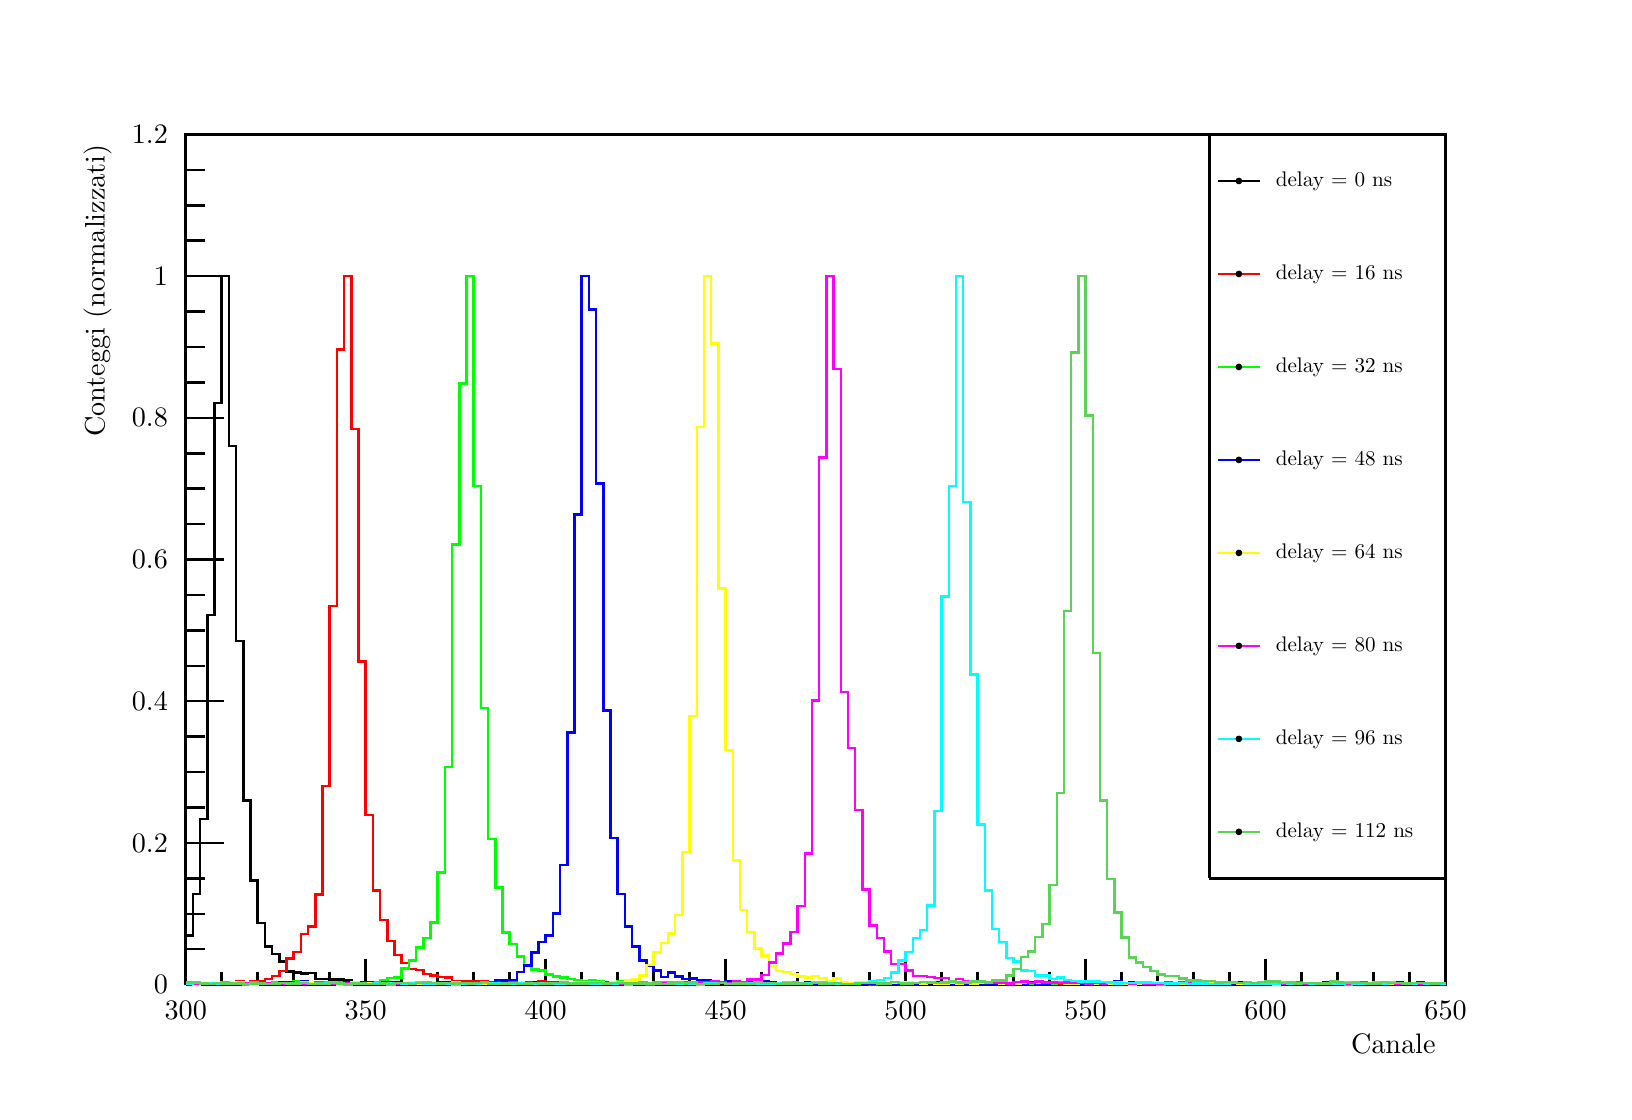
\begin{tikzpicture}
\pgfdeclareplotmark{cross} {
\pgfpathmoveto{\pgfpoint{-0.3\pgfplotmarksize}{\pgfplotmarksize}}
\pgfpathlineto{\pgfpoint{+0.3\pgfplotmarksize}{\pgfplotmarksize}}
\pgfpathlineto{\pgfpoint{+0.3\pgfplotmarksize}{0.3\pgfplotmarksize}}
\pgfpathlineto{\pgfpoint{+1\pgfplotmarksize}{0.3\pgfplotmarksize}}
\pgfpathlineto{\pgfpoint{+1\pgfplotmarksize}{-0.3\pgfplotmarksize}}
\pgfpathlineto{\pgfpoint{+0.3\pgfplotmarksize}{-0.3\pgfplotmarksize}}
\pgfpathlineto{\pgfpoint{+0.3\pgfplotmarksize}{-1.\pgfplotmarksize}}
\pgfpathlineto{\pgfpoint{-0.3\pgfplotmarksize}{-1.\pgfplotmarksize}}
\pgfpathlineto{\pgfpoint{-0.3\pgfplotmarksize}{-0.3\pgfplotmarksize}}
\pgfpathlineto{\pgfpoint{-1.\pgfplotmarksize}{-0.3\pgfplotmarksize}}
\pgfpathlineto{\pgfpoint{-1.\pgfplotmarksize}{0.3\pgfplotmarksize}}
\pgfpathlineto{\pgfpoint{-0.3\pgfplotmarksize}{0.3\pgfplotmarksize}}
\pgfpathclose
\pgfusepathqstroke
}
\pgfdeclareplotmark{cross*} {
\pgfpathmoveto{\pgfpoint{-0.3\pgfplotmarksize}{\pgfplotmarksize}}
\pgfpathlineto{\pgfpoint{+0.3\pgfplotmarksize}{\pgfplotmarksize}}
\pgfpathlineto{\pgfpoint{+0.3\pgfplotmarksize}{0.3\pgfplotmarksize}}
\pgfpathlineto{\pgfpoint{+1\pgfplotmarksize}{0.3\pgfplotmarksize}}
\pgfpathlineto{\pgfpoint{+1\pgfplotmarksize}{-0.3\pgfplotmarksize}}
\pgfpathlineto{\pgfpoint{+0.3\pgfplotmarksize}{-0.3\pgfplotmarksize}}
\pgfpathlineto{\pgfpoint{+0.3\pgfplotmarksize}{-1.\pgfplotmarksize}}
\pgfpathlineto{\pgfpoint{-0.3\pgfplotmarksize}{-1.\pgfplotmarksize}}
\pgfpathlineto{\pgfpoint{-0.3\pgfplotmarksize}{-0.3\pgfplotmarksize}}
\pgfpathlineto{\pgfpoint{-1.\pgfplotmarksize}{-0.3\pgfplotmarksize}}
\pgfpathlineto{\pgfpoint{-1.\pgfplotmarksize}{0.3\pgfplotmarksize}}
\pgfpathlineto{\pgfpoint{-0.3\pgfplotmarksize}{0.3\pgfplotmarksize}}
\pgfpathclose
\pgfusepathqfillstroke
}
\pgfdeclareplotmark{newstar} {
\pgfpathmoveto{\pgfqpoint{0pt}{\pgfplotmarksize}}
\pgfpathlineto{\pgfqpointpolar{44}{0.5\pgfplotmarksize}}
\pgfpathlineto{\pgfqpointpolar{18}{\pgfplotmarksize}}
\pgfpathlineto{\pgfqpointpolar{-20}{0.5\pgfplotmarksize}}
\pgfpathlineto{\pgfqpointpolar{-54}{\pgfplotmarksize}}
\pgfpathlineto{\pgfqpointpolar{-90}{0.5\pgfplotmarksize}}
\pgfpathlineto{\pgfqpointpolar{234}{\pgfplotmarksize}}
\pgfpathlineto{\pgfqpointpolar{198}{0.5\pgfplotmarksize}}
\pgfpathlineto{\pgfqpointpolar{162}{\pgfplotmarksize}}
\pgfpathlineto{\pgfqpointpolar{134}{0.5\pgfplotmarksize}}
\pgfpathclose
\pgfusepathqstroke
}
\pgfdeclareplotmark{newstar*} {
\pgfpathmoveto{\pgfqpoint{0pt}{\pgfplotmarksize}}
\pgfpathlineto{\pgfqpointpolar{44}{0.5\pgfplotmarksize}}
\pgfpathlineto{\pgfqpointpolar{18}{\pgfplotmarksize}}
\pgfpathlineto{\pgfqpointpolar{-20}{0.5\pgfplotmarksize}}
\pgfpathlineto{\pgfqpointpolar{-54}{\pgfplotmarksize}}
\pgfpathlineto{\pgfqpointpolar{-90}{0.5\pgfplotmarksize}}
\pgfpathlineto{\pgfqpointpolar{234}{\pgfplotmarksize}}
\pgfpathlineto{\pgfqpointpolar{198}{0.5\pgfplotmarksize}}
\pgfpathlineto{\pgfqpointpolar{162}{\pgfplotmarksize}}
\pgfpathlineto{\pgfqpointpolar{134}{0.5\pgfplotmarksize}}
\pgfpathclose
\pgfusepathqfillstroke
}
\definecolor{c}{rgb}{1,1,1};
\draw [color=c, fill=c] (0,0) rectangle (20,13.4957);
\draw [color=c, fill=c] (2,1.34957) rectangle (18,12.1461);
\definecolor{c}{rgb}{0,0,0};
\draw [c,line width=0.9] (2,1.34957) -- (2,12.1461) -- (18,12.1461) -- (18,1.34957) -- (2,1.34957);
\definecolor{c}{rgb}{1,1,1};
\draw [color=c, fill=c] (2,1.34957) rectangle (18,12.1461);
\definecolor{c}{rgb}{0,0,0};
\draw [c,line width=0.9] (2,1.34957) -- (2,12.1461) -- (18,12.1461) -- (18,1.34957) -- (2,1.34957);
\draw [c,line width=0.9] (2,1.97502) -- (2.09143,1.97502) -- (2.09143,2.50101) -- (2.18286,2.50101) -- (2.18286,3.45575) -- (2.27429,3.45575) -- (2.27429,6.04373) -- (2.36571,6.04373) -- (2.36571,8.73336) -- (2.45714,8.73336) -- (2.45714,10.3467) --
 (2.54857,10.3467) -- (2.54857,8.18969) -- (2.64,8.18969) -- (2.64,5.71664) -- (2.73143,5.71664) -- (2.73143,3.6856) -- (2.82286,3.6856) -- (2.82286,2.67118) -- (2.91429,2.67118) -- (2.91429,2.13414) -- (3.00571,2.13414) -- (3.00571,1.83578) --
 (3.09714,1.83578) -- (3.09714,1.73854) -- (3.18857,1.73854) -- (3.18857,1.64351) -- (3.28,1.64351) -- (3.28,1.51532) -- (3.37143,1.51532) -- (3.37143,1.50206) -- (3.46286,1.50206) -- (3.46286,1.49101) -- (3.55429,1.49101) -- (3.55429,1.49764) --
 (3.64571,1.49764) -- (3.64571,1.4225) -- (3.73714,1.4225) -- (3.73714,1.42029) -- (3.82857,1.42029) -- (3.82857,1.41366) -- (3.92,1.41366) -- (3.92,1.41587) -- (4.01143,1.41587) -- (4.01143,1.40482) -- (4.10286,1.40482) -- (4.10286,1.38493) --
 (4.19429,1.38493) -- (4.19429,1.38493) -- (4.28571,1.38493) -- (4.28571,1.37167) -- (4.37714,1.37167) -- (4.37714,1.38272) -- (4.46857,1.38272) -- (4.46857,1.37609) -- (4.56,1.37609) -- (4.56,1.38493) -- (4.65143,1.38493) -- (4.65143,1.37609) --
 (4.74286,1.37609) -- (4.74286,1.36946) -- (4.83429,1.36946) -- (4.83429,1.37388) -- (4.92571,1.37388) -- (4.92571,1.36504) -- (5.01714,1.36504) -- (5.01714,1.37167) -- (5.10857,1.37167) -- (5.10857,1.36946) -- (5.2,1.36946) -- (5.2,1.37609) --
 (5.29143,1.37609) -- (5.29143,1.36946) -- (5.38286,1.36946) -- (5.38286,1.37609) -- (5.47429,1.37609) -- (5.47429,1.37167) -- (5.56571,1.37167) -- (5.56571,1.36946) -- (5.65714,1.36946) -- (5.65714,1.35399) -- (5.74857,1.35399) -- (5.74857,1.36946)
 -- (5.84,1.36946) -- (5.84,1.36062) -- (5.93143,1.36062) -- (5.93143,1.36504) -- (6.02286,1.36504) -- (6.02286,1.36946) -- (6.11429,1.36946) -- (6.11429,1.36062) -- (6.20571,1.36062) -- (6.20571,1.36504) -- (6.29714,1.36504) -- (6.29714,1.36725) --
 (6.38857,1.36725) -- (6.38857,1.37388) -- (6.48,1.37388) -- (6.48,1.36946) -- (6.57143,1.36946) -- (6.57143,1.36283) -- (6.66286,1.36283) -- (6.66286,1.36946) -- (6.75429,1.36946) -- (6.75429,1.3783) -- (6.84571,1.3783) -- (6.84571,1.36946) --
 (6.93714,1.36946) -- (6.93714,1.37167) -- (7.02857,1.37167) -- (7.02857,1.37609) -- (7.12,1.37609) -- (7.12,1.3783) -- (7.21143,1.3783) -- (7.21143,1.36283) -- (7.30286,1.36283) -- (7.30286,1.37167) -- (7.39429,1.37167) -- (7.39429,1.37167) --
 (7.48571,1.37167) -- (7.48571,1.37388) -- (7.57714,1.37388) -- (7.57714,1.35399) -- (7.66857,1.35399) -- (7.66857,1.37167) -- (7.76,1.37167) -- (7.76,1.36725) -- (7.85143,1.36725) -- (7.85143,1.36946) -- (7.94286,1.36946) -- (7.94286,1.37609) --
 (8.03429,1.37609) -- (8.03429,1.36504) -- (8.12571,1.36504) -- (8.12571,1.3562) -- (8.21714,1.3562) -- (8.21714,1.35841) -- (8.30857,1.35841) -- (8.30857,1.36504) -- (8.4,1.36504) -- (8.4,1.36283) -- (8.49143,1.36283) -- (8.49143,1.36504) --
 (8.58286,1.36504) -- (8.58286,1.3783) -- (8.67429,1.3783) -- (8.67429,1.36504) -- (8.76571,1.36504) -- (8.76571,1.36725) -- (8.85714,1.36725) -- (8.85714,1.36062) -- (8.94857,1.36062) -- (8.94857,1.36062) -- (9.04,1.36062) -- (9.04,1.37167) --
 (9.13143,1.37167) -- (9.13143,1.36946) -- (9.22286,1.36946) -- (9.22286,1.36725) -- (9.31429,1.36725) -- (9.31429,1.36725) -- (9.40571,1.36725) -- (9.40571,1.37167) -- (9.49714,1.37167) -- (9.49714,1.36725) -- (9.58857,1.36725) -- (9.58857,1.36504)
 -- (9.68,1.36504) -- (9.68,1.36283) -- (9.77143,1.36283) -- (9.77143,1.36283) -- (9.86286,1.36283) -- (9.86286,1.36062) -- (9.95429,1.36062) -- (9.95429,1.36062) -- (10.0457,1.36062) -- (10.0457,1.36283) -- (10.1371,1.36283) -- (10.1371,1.37609) --
 (10.2286,1.37609) -- (10.2286,1.36725) -- (10.32,1.36725) -- (10.32,1.35841) -- (10.4114,1.35841) -- (10.4114,1.36283) -- (10.5029,1.36283) -- (10.5029,1.36062) -- (10.5943,1.36062) -- (10.5943,1.36504) -- (10.6857,1.36504) -- (10.6857,1.36504) --
 (10.7771,1.36504) -- (10.7771,1.36946) -- (10.8686,1.36946) -- (10.8686,1.37167) -- (10.96,1.37167) -- (10.96,1.36946) -- (11.0514,1.36946) -- (11.0514,1.35399) -- (11.1429,1.35399) -- (11.1429,1.36283) -- (11.2343,1.36283) -- (11.2343,1.35841) --
 (11.3257,1.35841) -- (11.3257,1.36725) -- (11.4171,1.36725) -- (11.4171,1.36504) -- (11.5086,1.36504) -- (11.5086,1.37167) -- (11.6,1.37167) -- (11.6,1.36062) -- (11.6914,1.36062) -- (11.6914,1.35399) -- (11.7829,1.35399) -- (11.7829,1.36504) --
 (11.8743,1.36504) -- (11.8743,1.3562) -- (11.9657,1.3562) -- (11.9657,1.35841) -- (12.0571,1.35841) -- (12.0571,1.3783) -- (12.1486,1.3783) -- (12.1486,1.36062) -- (12.24,1.36062) -- (12.24,1.36283) -- (12.3314,1.36283) -- (12.3314,1.36725) --
 (12.4229,1.36725) -- (12.4229,1.36725) -- (12.5143,1.36725) -- (12.5143,1.37609) -- (12.6057,1.37609) -- (12.6057,1.36504) -- (12.6971,1.36504) -- (12.6971,1.36725) -- (12.7886,1.36725) -- (12.7886,1.36504) -- (12.88,1.36504) -- (12.88,1.36283) --
 (12.9714,1.36283) -- (12.9714,1.36725) -- (13.0629,1.36725) -- (13.0629,1.3562) -- (13.1543,1.3562) -- (13.1543,1.36946) -- (13.2457,1.36946) -- (13.2457,1.36283) -- (13.3371,1.36283) -- (13.3371,1.36062) -- (13.4286,1.36062) -- (13.4286,1.36283) --
 (13.52,1.36283) -- (13.52,1.35178) -- (13.6114,1.35178) -- (13.6114,1.36946) -- (13.7029,1.36946) -- (13.7029,1.36062) -- (13.7943,1.36062) -- (13.7943,1.36946) -- (13.8857,1.36946) -- (13.8857,1.36283) -- (13.9771,1.36283) -- (13.9771,1.37609) --
 (14.0686,1.37609) -- (14.0686,1.36504) -- (14.16,1.36504) -- (14.16,1.37167) -- (14.2514,1.37167) -- (14.2514,1.37167) -- (14.3429,1.37167) -- (14.3429,1.36062) -- (14.4343,1.36062) -- (14.4343,1.3562) -- (14.5257,1.3562) -- (14.5257,1.36283) --
 (14.6171,1.36283) -- (14.6171,1.35841) -- (14.7086,1.35841) -- (14.7086,1.36946) -- (14.8,1.36946) -- (14.8,1.36504) -- (14.8914,1.36504) -- (14.8914,1.37609) -- (14.9829,1.37609) -- (14.9829,1.35841) -- (15.0743,1.35841) -- (15.0743,1.3562) --
 (15.1657,1.3562) -- (15.1657,1.36946) -- (15.2571,1.36946) -- (15.2571,1.36283) -- (15.3486,1.36283) -- (15.3486,1.37609) -- (15.44,1.37609) -- (15.44,1.36504) -- (15.5314,1.36504) -- (15.5314,1.36283) -- (15.6229,1.36283) -- (15.6229,1.36283) --
 (15.7143,1.36283) -- (15.7143,1.36946) -- (15.8057,1.36946) -- (15.8057,1.36283) -- (15.8971,1.36283) -- (15.8971,1.35841) -- (15.9886,1.35841) -- (15.9886,1.36725) -- (16.08,1.36725) -- (16.08,1.36283) -- (16.1714,1.36283) -- (16.1714,1.36725) --
 (16.2629,1.36725) -- (16.2629,1.35841) -- (16.3543,1.35841) -- (16.3543,1.36725) -- (16.4457,1.36725) -- (16.4457,1.37388) -- (16.5371,1.37388) -- (16.5371,1.36725) -- (16.6286,1.36725) -- (16.6286,1.37388) -- (16.72,1.37388) -- (16.72,1.37609) --
 (16.8114,1.37609) -- (16.8114,1.37388) -- (16.9029,1.37388) -- (16.9029,1.36283) -- (16.9943,1.36283) -- (16.9943,1.37167) -- (17.0857,1.37167) -- (17.0857,1.36062) -- (17.1771,1.36062) -- (17.1771,1.36283) -- (17.2686,1.36283) -- (17.2686,1.37388)
 -- (17.36,1.37388) -- (17.36,1.35841) -- (17.4514,1.35841) -- (17.4514,1.36283) -- (17.5429,1.36283) -- (17.5429,1.36946) -- (17.6343,1.36946) -- (17.6343,1.36283) -- (17.7257,1.36283) -- (17.7257,1.36946) -- (17.8171,1.36946) -- (17.8171,1.36946)
 -- (17.9086,1.36946) -- (17.9086,1.36504) -- (18,1.36504);
\draw [c,line width=0.9] (2,1.34957) -- (18,1.34957);
\draw [anchor= east] (18,0.593811) node[scale=1.01821, color=c, rotate=0]{Canale};
\draw [c,line width=0.9] (2,1.67347) -- (2,1.34957);
\draw [c,line width=0.9] (2.45714,1.51152) -- (2.45714,1.34957);
\draw [c,line width=0.9] (2.91429,1.51152) -- (2.91429,1.34957);
\draw [c,line width=0.9] (3.37143,1.51152) -- (3.37143,1.34957);
\draw [c,line width=0.9] (3.82857,1.51152) -- (3.82857,1.34957);
\draw [c,line width=0.9] (4.28571,1.67347) -- (4.28571,1.34957);
\draw [c,line width=0.9] (4.74286,1.51152) -- (4.74286,1.34957);
\draw [c,line width=0.9] (5.2,1.51152) -- (5.2,1.34957);
\draw [c,line width=0.9] (5.65714,1.51152) -- (5.65714,1.34957);
\draw [c,line width=0.9] (6.11429,1.51152) -- (6.11429,1.34957);
\draw [c,line width=0.9] (6.57143,1.67347) -- (6.57143,1.34957);
\draw [c,line width=0.9] (7.02857,1.51152) -- (7.02857,1.34957);
\draw [c,line width=0.9] (7.48571,1.51152) -- (7.48571,1.34957);
\draw [c,line width=0.9] (7.94286,1.51152) -- (7.94286,1.34957);
\draw [c,line width=0.9] (8.4,1.51152) -- (8.4,1.34957);
\draw [c,line width=0.9] (8.85714,1.67347) -- (8.85714,1.34957);
\draw [c,line width=0.9] (9.31429,1.51152) -- (9.31429,1.34957);
\draw [c,line width=0.9] (9.77143,1.51152) -- (9.77143,1.34957);
\draw [c,line width=0.9] (10.2286,1.51152) -- (10.2286,1.34957);
\draw [c,line width=0.9] (10.6857,1.51152) -- (10.6857,1.34957);
\draw [c,line width=0.9] (11.1429,1.67347) -- (11.1429,1.34957);
\draw [c,line width=0.9] (11.6,1.51152) -- (11.6,1.34957);
\draw [c,line width=0.9] (12.0571,1.51152) -- (12.0571,1.34957);
\draw [c,line width=0.9] (12.5143,1.51152) -- (12.5143,1.34957);
\draw [c,line width=0.9] (12.9714,1.51152) -- (12.9714,1.34957);
\draw [c,line width=0.9] (13.4286,1.67347) -- (13.4286,1.34957);
\draw [c,line width=0.9] (13.8857,1.51152) -- (13.8857,1.34957);
\draw [c,line width=0.9] (14.3429,1.51152) -- (14.3429,1.34957);
\draw [c,line width=0.9] (14.8,1.51152) -- (14.8,1.34957);
\draw [c,line width=0.9] (15.2571,1.51152) -- (15.2571,1.34957);
\draw [c,line width=0.9] (15.7143,1.67347) -- (15.7143,1.34957);
\draw [c,line width=0.9] (16.1714,1.51152) -- (16.1714,1.34957);
\draw [c,line width=0.9] (16.6286,1.51152) -- (16.6286,1.34957);
\draw [c,line width=0.9] (17.0857,1.51152) -- (17.0857,1.34957);
\draw [c,line width=0.9] (17.5429,1.51152) -- (17.5429,1.34957);
\draw [c,line width=0.9] (18,1.67347) -- (18,1.34957);
\draw [anchor=base] (2,0.904212) node[scale=1.01821, color=c, rotate=0]{300};
\draw [anchor=base] (4.28571,0.904212) node[scale=1.01821, color=c, rotate=0]{350};
\draw [anchor=base] (6.57143,0.904212) node[scale=1.01821, color=c, rotate=0]{400};
\draw [anchor=base] (8.85714,0.904212) node[scale=1.01821, color=c, rotate=0]{450};
\draw [anchor=base] (11.1429,0.904212) node[scale=1.01821, color=c, rotate=0]{500};
\draw [anchor=base] (13.4286,0.904212) node[scale=1.01821, color=c, rotate=0]{550};
\draw [anchor=base] (15.7143,0.904212) node[scale=1.01821, color=c, rotate=0]{600};
\draw [anchor=base] (18,0.904212) node[scale=1.01821, color=c, rotate=0]{650};
\draw [c,line width=0.9] (2,1.34957) -- (2,12.1461);
\draw [anchor= east] (0.88,12.1461) node[scale=1.01821, color=c, rotate=90]{Conteggi (normalizzati)};
\draw [c,line width=0.9] (2.48,1.34957) -- (2,1.34957);
\draw [c,line width=0.9] (2.24,1.79943) -- (2,1.79943);
\draw [c,line width=0.9] (2.24,2.24928) -- (2,2.24928);
\draw [c,line width=0.9] (2.24,2.69914) -- (2,2.69914);
\draw [c,line width=0.9] (2.48,3.149) -- (2,3.149);
\draw [c,line width=0.9] (2.24,3.59885) -- (2,3.59885);
\draw [c,line width=0.9] (2.24,4.04871) -- (2,4.04871);
\draw [c,line width=0.9] (2.24,4.49857) -- (2,4.49857);
\draw [c,line width=0.9] (2.48,4.94842) -- (2,4.94842);
\draw [c,line width=0.9] (2.24,5.39828) -- (2,5.39828);
\draw [c,line width=0.9] (2.24,5.84814) -- (2,5.84814);
\draw [c,line width=0.9] (2.24,6.29799) -- (2,6.29799);
\draw [c,line width=0.9] (2.48,6.74785) -- (2,6.74785);
\draw [c,line width=0.9] (2.24,7.19771) -- (2,7.19771);
\draw [c,line width=0.9] (2.24,7.64756) -- (2,7.64756);
\draw [c,line width=0.9] (2.24,8.09742) -- (2,8.09742);
\draw [c,line width=0.9] (2.48,8.54728) -- (2,8.54728);
\draw [c,line width=0.9] (2.24,8.99713) -- (2,8.99713);
\draw [c,line width=0.9] (2.24,9.44699) -- (2,9.44699);
\draw [c,line width=0.9] (2.24,9.89685) -- (2,9.89685);
\draw [c,line width=0.9] (2.48,10.3467) -- (2,10.3467);
\draw [c,line width=0.9] (2.24,10.7966) -- (2,10.7966);
\draw [c,line width=0.9] (2.24,11.2464) -- (2,11.2464);
\draw [c,line width=0.9] (2.24,11.6963) -- (2,11.6963);
\draw [c,line width=0.9] (2.48,12.1461) -- (2,12.1461);
\draw [c,line width=0.9] (2.48,12.1461) -- (2,12.1461);
\draw [anchor= east] (1.9,1.34957) node[scale=1.01821, color=c, rotate=0]{0};
\draw [anchor= east] (1.9,3.149) node[scale=1.01821, color=c, rotate=0]{0.2};
\draw [anchor= east] (1.9,4.94842) node[scale=1.01821, color=c, rotate=0]{0.4};
\draw [anchor= east] (1.9,6.74785) node[scale=1.01821, color=c, rotate=0]{0.6};
\draw [anchor= east] (1.9,8.54728) node[scale=1.01821, color=c, rotate=0]{0.8};
\draw [anchor= east] (1.9,10.3467) node[scale=1.01821, color=c, rotate=0]{1};
\draw [anchor= east] (1.9,12.1461) node[scale=1.01821, color=c, rotate=0]{1.2};
\definecolor{c}{rgb}{1,0,0};
\draw [c,line width=0.9] (2,1.37694) -- (2.09143,1.37694) -- (2.09143,1.38151) -- (2.18286,1.38151) -- (2.18286,1.37238) -- (2.27429,1.37238) -- (2.27429,1.37238) -- (2.36571,1.37238) -- (2.36571,1.3701) -- (2.45714,1.3701) -- (2.45714,1.37694) --
 (2.54857,1.37694) -- (2.54857,1.36326) -- (2.64,1.36326) -- (2.64,1.39063) -- (2.73143,1.39063) -- (2.73143,1.36326) -- (2.82286,1.36326) -- (2.82286,1.39519) -- (2.91429,1.39519) -- (2.91429,1.39519) -- (3.00571,1.39519) -- (3.00571,1.42257) --
 (3.09714,1.42257) -- (3.09714,1.45907) -- (3.18857,1.45907) -- (3.18857,1.52066) -- (3.28,1.52066) -- (3.28,1.68035) -- (3.37143,1.68035) -- (3.37143,1.76475) -- (3.46286,1.76475) -- (3.46286,1.99287) -- (3.55429,1.99287) -- (3.55429,2.08869) --
 (3.64571,2.08869) -- (3.64571,2.49702) -- (3.73714,2.49702) -- (3.73714,3.87032) -- (3.82857,3.87032) -- (3.82857,6.1561) -- (3.92,6.1561) -- (3.92,9.41597) -- (4.01143,9.41597) -- (4.01143,10.3467) -- (4.10286,10.3467) -- (4.10286,8.4031) --
 (4.19429,8.4031) -- (4.19429,5.45349) -- (4.28571,5.45349) -- (4.28571,3.50304) -- (4.37714,3.50304) -- (4.37714,2.54265) -- (4.46857,2.54265) -- (4.46857,2.17081) -- (4.56,2.17081) -- (4.56,1.90163) -- (4.65143,1.90163) -- (4.65143,1.72597) --
 (4.74286,1.72597) -- (4.74286,1.62104) -- (4.83429,1.62104) -- (4.83429,1.54576) -- (4.92571,1.54576) -- (4.92571,1.53207) -- (5.01714,1.53207) -- (5.01714,1.48644) -- (5.10857,1.48644) -- (5.10857,1.46363) -- (5.2,1.46363) -- (5.2,1.4431) --
 (5.29143,1.4431) -- (5.29143,1.44082) -- (5.38286,1.44082) -- (5.38286,1.39748) -- (5.47429,1.39748) -- (5.47429,1.39291) -- (5.56571,1.39291) -- (5.56571,1.38835) -- (5.65714,1.38835) -- (5.65714,1.39748) -- (5.74857,1.39748) -- (5.74857,1.39291)
 -- (5.84,1.39291) -- (5.84,1.38151) -- (5.93143,1.38151) -- (5.93143,1.38835) -- (6.02286,1.38835) -- (6.02286,1.38607) -- (6.11429,1.38607) -- (6.11429,1.38151) -- (6.20571,1.38151) -- (6.20571,1.38151) -- (6.29714,1.38151) -- (6.29714,1.37466) --
 (6.38857,1.37466) -- (6.38857,1.3701) -- (6.48,1.3701) -- (6.48,1.38835) -- (6.57143,1.38835) -- (6.57143,1.37694) -- (6.66286,1.37694) -- (6.66286,1.37466) -- (6.75429,1.37466) -- (6.75429,1.36782) -- (6.84571,1.36782) -- (6.84571,1.3587) --
 (6.93714,1.3587) -- (6.93714,1.3701) -- (7.02857,1.3701) -- (7.02857,1.36098) -- (7.12,1.36098) -- (7.12,1.36326) -- (7.21143,1.36326) -- (7.21143,1.36782) -- (7.30286,1.36782) -- (7.30286,1.37694) -- (7.39429,1.37694) -- (7.39429,1.37238) --
 (7.48571,1.37238) -- (7.48571,1.35641) -- (7.57714,1.35641) -- (7.57714,1.37238) -- (7.66857,1.37238) -- (7.66857,1.37238) -- (7.76,1.37238) -- (7.76,1.36098) -- (7.85143,1.36098) -- (7.85143,1.37238) -- (7.94286,1.37238) -- (7.94286,1.36782) --
 (8.03429,1.36782) -- (8.03429,1.36554) -- (8.12571,1.36554) -- (8.12571,1.36098) -- (8.21714,1.36098) -- (8.21714,1.3701) -- (8.30857,1.3701) -- (8.30857,1.36326) -- (8.4,1.36326) -- (8.4,1.37238) -- (8.49143,1.37238) -- (8.49143,1.3701) --
 (8.58286,1.3701) -- (8.58286,1.36326) -- (8.67429,1.36326) -- (8.67429,1.36782) -- (8.76571,1.36782) -- (8.76571,1.36782) -- (8.85714,1.36782) -- (8.85714,1.36554) -- (8.94857,1.36554) -- (8.94857,1.36326) -- (9.04,1.36326) -- (9.04,1.3587) --
 (9.13143,1.3587) -- (9.13143,1.3701) -- (9.22286,1.3701) -- (9.22286,1.36782) -- (9.31429,1.36782) -- (9.31429,1.36782) -- (9.40571,1.36782) -- (9.40571,1.37466) -- (9.49714,1.37466) -- (9.49714,1.3587) -- (9.58857,1.3587) -- (9.58857,1.36782) --
 (9.68,1.36782) -- (9.68,1.37238) -- (9.77143,1.37238) -- (9.77143,1.36782) -- (9.86286,1.36782) -- (9.86286,1.36326) -- (9.95429,1.36326) -- (9.95429,1.37923) -- (10.0457,1.37923) -- (10.0457,1.36554) -- (10.1371,1.36554) -- (10.1371,1.36326) --
 (10.2286,1.36326) -- (10.2286,1.36326) -- (10.32,1.36326) -- (10.32,1.36098) -- (10.4114,1.36098) -- (10.4114,1.36326) -- (10.5029,1.36326) -- (10.5029,1.37466) -- (10.5943,1.37466) -- (10.5943,1.36782) -- (10.6857,1.36782) -- (10.6857,1.35413) --
 (10.7771,1.35413) -- (10.7771,1.36554) -- (10.8686,1.36554) -- (10.8686,1.37238) -- (10.96,1.37238) -- (10.96,1.36098) -- (11.0514,1.36098) -- (11.0514,1.36326) -- (11.1429,1.36326) -- (11.1429,1.36326) -- (11.2343,1.36326) -- (11.2343,1.36326) --
 (11.3257,1.36326) -- (11.3257,1.38151) -- (11.4171,1.38151) -- (11.4171,1.36782) -- (11.5086,1.36782) -- (11.5086,1.36782) -- (11.6,1.36782) -- (11.6,1.38151) -- (11.6914,1.38151) -- (11.6914,1.36098) -- (11.7829,1.36098) -- (11.7829,1.37238) --
 (11.8743,1.37238) -- (11.8743,1.36326) -- (11.9657,1.36326) -- (11.9657,1.36554) -- (12.0571,1.36554) -- (12.0571,1.36326) -- (12.1486,1.36326) -- (12.1486,1.36326) -- (12.24,1.36326) -- (12.24,1.36554) -- (12.3314,1.36554) -- (12.3314,1.36554) --
 (12.4229,1.36554) -- (12.4229,1.36782) -- (12.5143,1.36782) -- (12.5143,1.3587) -- (12.6057,1.3587) -- (12.6057,1.36554) -- (12.6971,1.36554) -- (12.6971,1.36098) -- (12.7886,1.36098) -- (12.7886,1.37923) -- (12.88,1.37923) -- (12.88,1.3701) --
 (12.9714,1.3701) -- (12.9714,1.37466) -- (13.0629,1.37466) -- (13.0629,1.36098) -- (13.1543,1.36098) -- (13.1543,1.36098) -- (13.2457,1.36098) -- (13.2457,1.3701) -- (13.3371,1.3701) -- (13.3371,1.3701) -- (13.4286,1.3701) -- (13.4286,1.37694) --
 (13.52,1.37694) -- (13.52,1.36098) -- (13.6114,1.36098) -- (13.6114,1.36326) -- (13.7029,1.36326) -- (13.7029,1.37238) -- (13.7943,1.37238) -- (13.7943,1.37923) -- (13.8857,1.37923) -- (13.8857,1.36326) -- (13.9771,1.36326) -- (13.9771,1.35413) --
 (14.0686,1.35413) -- (14.0686,1.37238) -- (14.16,1.37238) -- (14.16,1.36554) -- (14.2514,1.36554) -- (14.2514,1.36782) -- (14.3429,1.36782) -- (14.3429,1.3587) -- (14.4343,1.3587) -- (14.4343,1.3587) -- (14.5257,1.3587) -- (14.5257,1.36098) --
 (14.6171,1.36098) -- (14.6171,1.3701) -- (14.7086,1.3701) -- (14.7086,1.3701) -- (14.8,1.3701) -- (14.8,1.36326) -- (14.8914,1.36326) -- (14.8914,1.37238) -- (14.9829,1.37238) -- (14.9829,1.3701) -- (15.0743,1.3701) -- (15.0743,1.36326) --
 (15.1657,1.36326) -- (15.1657,1.36782) -- (15.2571,1.36782) -- (15.2571,1.36326) -- (15.3486,1.36326) -- (15.3486,1.3587) -- (15.44,1.3587) -- (15.44,1.36782) -- (15.5314,1.36782) -- (15.5314,1.36554) -- (15.6229,1.36554) -- (15.6229,1.36098) --
 (15.7143,1.36098) -- (15.7143,1.36326) -- (15.8057,1.36326) -- (15.8057,1.36782) -- (15.8971,1.36782) -- (15.8971,1.36782) -- (15.9886,1.36782) -- (15.9886,1.36554) -- (16.08,1.36554) -- (16.08,1.37466) -- (16.1714,1.37466) -- (16.1714,1.36098) --
 (16.2629,1.36098) -- (16.2629,1.36782) -- (16.3543,1.36782) -- (16.3543,1.35641) -- (16.4457,1.35641) -- (16.4457,1.36554) -- (16.5371,1.36554) -- (16.5371,1.3701) -- (16.6286,1.3701) -- (16.6286,1.36326) -- (16.72,1.36326) -- (16.72,1.37238) --
 (16.8114,1.37238) -- (16.8114,1.36326) -- (16.9029,1.36326) -- (16.9029,1.36782) -- (16.9943,1.36782) -- (16.9943,1.37238) -- (17.0857,1.37238) -- (17.0857,1.36554) -- (17.1771,1.36554) -- (17.1771,1.36782) -- (17.2686,1.36782) -- (17.2686,1.37694)
 -- (17.36,1.37694) -- (17.36,1.36098) -- (17.4514,1.36098) -- (17.4514,1.3587) -- (17.5429,1.3587) -- (17.5429,1.36782) -- (17.6343,1.36782) -- (17.6343,1.36782) -- (17.7257,1.36782) -- (17.7257,1.3587) -- (17.8171,1.3587) -- (17.8171,1.3587) --
 (17.9086,1.3587) -- (17.9086,1.35641) -- (18,1.35641);
\definecolor{c}{rgb}{0,1,0};
\draw [c,line width=0.9] (2,1.37848) -- (2.09143,1.37848) -- (2.09143,1.36514) -- (2.18286,1.36514) -- (2.18286,1.35847) -- (2.27429,1.35847) -- (2.27429,1.36069) -- (2.36571,1.36069) -- (2.36571,1.36514) -- (2.45714,1.36514) -- (2.45714,1.37848) --
 (2.54857,1.37848) -- (2.54857,1.36514) -- (2.64,1.36514) -- (2.64,1.36958) -- (2.73143,1.36958) -- (2.73143,1.35402) -- (2.82286,1.35402) -- (2.82286,1.37403) -- (2.91429,1.37403) -- (2.91429,1.36736) -- (3.00571,1.36736) -- (3.00571,1.35624) --
 (3.09714,1.35624) -- (3.09714,1.37625) -- (3.18857,1.37625) -- (3.18857,1.36958) -- (3.28,1.36958) -- (3.28,1.36736) -- (3.37143,1.36736) -- (3.37143,1.38737) -- (3.46286,1.38737) -- (3.46286,1.37848) -- (3.55429,1.37848) -- (3.55429,1.36514) --
 (3.64571,1.36514) -- (3.64571,1.37848) -- (3.73714,1.37848) -- (3.73714,1.37403) -- (3.82857,1.37403) -- (3.82857,1.36958) -- (3.92,1.36958) -- (3.92,1.3807) -- (4.01143,1.3807) -- (4.01143,1.38293) -- (4.10286,1.38293) -- (4.10286,1.36514) --
 (4.19429,1.36514) -- (4.19429,1.36069) -- (4.28571,1.36069) -- (4.28571,1.37625) -- (4.37714,1.37625) -- (4.37714,1.38293) -- (4.46857,1.38293) -- (4.46857,1.40961) -- (4.56,1.40961) -- (4.56,1.4363) -- (4.65143,1.4363) -- (4.65143,1.44074) --
 (4.74286,1.44074) -- (4.74286,1.55415) -- (4.83429,1.55415) -- (4.83429,1.65867) -- (4.92571,1.65867) -- (4.92571,1.821) -- (5.01714,1.821) -- (5.01714,1.9433) -- (5.10857,1.9433) -- (5.10857,2.14121) -- (5.2,2.14121) -- (5.2,2.77497) --
 (5.29143,2.77497) -- (5.29143,4.11364) -- (5.38286,4.11364) -- (5.38286,6.93776) -- (5.47429,6.93776) -- (5.47429,8.98135) -- (5.56571,8.98135) -- (5.56571,10.3467) -- (5.65714,10.3467) -- (5.65714,7.68048) -- (5.74857,7.68048) -- (5.74857,4.86081)
 -- (5.84,4.86081) -- (5.84,3.20192) -- (5.93143,3.20192) -- (5.93143,2.58151) -- (6.02286,2.58151) -- (6.02286,2.01446) -- (6.11429,2.01446) -- (6.11429,1.86769) -- (6.20571,1.86769) -- (6.20571,1.70759) -- (6.29714,1.70759) -- (6.29714,1.60085) --
 (6.38857,1.60085) -- (6.38857,1.53859) -- (6.48,1.53859) -- (6.48,1.52747) -- (6.57143,1.52747) -- (6.57143,1.48077) -- (6.66286,1.48077) -- (6.66286,1.45186) -- (6.75429,1.45186) -- (6.75429,1.44297) -- (6.84571,1.44297) -- (6.84571,1.42073) --
 (6.93714,1.42073) -- (6.93714,1.40516) -- (7.02857,1.40516) -- (7.02857,1.39849) -- (7.12,1.39849) -- (7.12,1.40072) -- (7.21143,1.40072) -- (7.21143,1.39627) -- (7.30286,1.39627) -- (7.30286,1.37181) -- (7.39429,1.37181) -- (7.39429,1.3807) --
 (7.48571,1.3807) -- (7.48571,1.38737) -- (7.57714,1.38737) -- (7.57714,1.3896) -- (7.66857,1.3896) -- (7.66857,1.36958) -- (7.76,1.36958) -- (7.76,1.38293) -- (7.85143,1.38293) -- (7.85143,1.37181) -- (7.94286,1.37181) -- (7.94286,1.37403) --
 (8.03429,1.37403) -- (8.03429,1.37403) -- (8.12571,1.37403) -- (8.12571,1.37848) -- (8.21714,1.37848) -- (8.21714,1.37625) -- (8.30857,1.37625) -- (8.30857,1.35847) -- (8.4,1.35847) -- (8.4,1.37403) -- (8.49143,1.37403) -- (8.49143,1.36514) --
 (8.58286,1.36514) -- (8.58286,1.36291) -- (8.67429,1.36291) -- (8.67429,1.36069) -- (8.76571,1.36069) -- (8.76571,1.37625) -- (8.85714,1.37625) -- (8.85714,1.37403) -- (8.94857,1.37403) -- (8.94857,1.36069) -- (9.04,1.36069) -- (9.04,1.36736) --
 (9.13143,1.36736) -- (9.13143,1.35847) -- (9.22286,1.35847) -- (9.22286,1.36736) -- (9.31429,1.36736) -- (9.31429,1.37403) -- (9.40571,1.37403) -- (9.40571,1.36069) -- (9.49714,1.36069) -- (9.49714,1.36291) -- (9.58857,1.36291) -- (9.58857,1.36736)
 -- (9.68,1.36736) -- (9.68,1.38293) -- (9.77143,1.38293) -- (9.77143,1.35847) -- (9.86286,1.35847) -- (9.86286,1.36291) -- (9.95429,1.36291) -- (9.95429,1.37403) -- (10.0457,1.37403) -- (10.0457,1.36069) -- (10.1371,1.36069) -- (10.1371,1.36736) --
 (10.2286,1.36736) -- (10.2286,1.35847) -- (10.32,1.35847) -- (10.32,1.36291) -- (10.4114,1.36291) -- (10.4114,1.36514) -- (10.5029,1.36514) -- (10.5029,1.35847) -- (10.5943,1.35847) -- (10.5943,1.37625) -- (10.6857,1.37625) -- (10.6857,1.36736) --
 (10.7771,1.36736) -- (10.7771,1.37403) -- (10.8686,1.37403) -- (10.8686,1.36736) -- (10.96,1.36736) -- (10.96,1.35624) -- (11.0514,1.35624) -- (11.0514,1.36291) -- (11.1429,1.36291) -- (11.1429,1.36958) -- (11.2343,1.36958) -- (11.2343,1.36291) --
 (11.3257,1.36291) -- (11.3257,1.35847) -- (11.4171,1.35847) -- (11.4171,1.37403) -- (11.5086,1.37403) -- (11.5086,1.36069) -- (11.6,1.36069) -- (11.6,1.36514) -- (11.6914,1.36514) -- (11.6914,1.37181) -- (11.7829,1.37181) -- (11.7829,1.37403) --
 (11.8743,1.37403) -- (11.8743,1.36291) -- (11.9657,1.36291) -- (11.9657,1.35624) -- (12.0571,1.35624) -- (12.0571,1.35847) -- (12.1486,1.35847) -- (12.1486,1.36514) -- (12.24,1.36514) -- (12.24,1.37181) -- (12.3314,1.37181) -- (12.3314,1.35847) --
 (12.4229,1.35847) -- (12.4229,1.36736) -- (12.5143,1.36736) -- (12.5143,1.36736) -- (12.6057,1.36736) -- (12.6057,1.37181) -- (12.6971,1.37181) -- (12.6971,1.36069) -- (12.7886,1.36069) -- (12.7886,1.36291) -- (12.88,1.36291) -- (12.88,1.36736) --
 (12.9714,1.36736) -- (12.9714,1.35624) -- (13.0629,1.35624) -- (13.0629,1.38293) -- (13.1543,1.38293) -- (13.1543,1.36291) -- (13.2457,1.36291) -- (13.2457,1.36069) -- (13.3371,1.36069) -- (13.3371,1.35847) -- (13.4286,1.35847) -- (13.4286,1.35847)
 -- (13.52,1.35847) -- (13.52,1.36958) -- (13.6114,1.36958) -- (13.6114,1.36958) -- (13.7029,1.36958) -- (13.7029,1.36069) -- (13.7943,1.36069) -- (13.7943,1.37181) -- (13.8857,1.37181) -- (13.8857,1.35847) -- (13.9771,1.35847) -- (13.9771,1.36514)
 -- (14.0686,1.36514) -- (14.0686,1.36291) -- (14.16,1.36291) -- (14.16,1.36069) -- (14.2514,1.36069) -- (14.2514,1.35624) -- (14.3429,1.35624) -- (14.3429,1.35179) -- (14.4343,1.35179) -- (14.4343,1.36069) -- (14.5257,1.36069) -- (14.5257,1.36069)
 -- (14.6171,1.36069) -- (14.6171,1.36291) -- (14.7086,1.36291) -- (14.7086,1.36958) -- (14.8,1.36958) -- (14.8,1.35624) -- (14.8914,1.35624) -- (14.8914,1.36736) -- (14.9829,1.36736) -- (14.9829,1.36736) -- (15.0743,1.36736) -- (15.0743,1.36958) --
 (15.1657,1.36958) -- (15.1657,1.36736) -- (15.2571,1.36736) -- (15.2571,1.37403) -- (15.3486,1.37403) -- (15.3486,1.36736) -- (15.44,1.36736) -- (15.44,1.36069) -- (15.5314,1.36069) -- (15.5314,1.36069) -- (15.6229,1.36069) -- (15.6229,1.36069) --
 (15.7143,1.36069) -- (15.7143,1.36514) -- (15.8057,1.36514) -- (15.8057,1.36736) -- (15.8971,1.36736) -- (15.8971,1.37181) -- (15.9886,1.37181) -- (15.9886,1.36736) -- (16.08,1.36736) -- (16.08,1.35624) -- (16.1714,1.35624) -- (16.1714,1.36291) --
 (16.2629,1.36291) -- (16.2629,1.36069) -- (16.3543,1.36069) -- (16.3543,1.36514) -- (16.4457,1.36514) -- (16.4457,1.36291) -- (16.5371,1.36291) -- (16.5371,1.36958) -- (16.6286,1.36958) -- (16.6286,1.37403) -- (16.72,1.37403) -- (16.72,1.35402) --
 (16.8114,1.35402) -- (16.8114,1.36291) -- (16.9029,1.36291) -- (16.9029,1.36514) -- (16.9943,1.36514) -- (16.9943,1.36291) -- (17.0857,1.36291) -- (17.0857,1.37181) -- (17.1771,1.37181) -- (17.1771,1.35624) -- (17.2686,1.35624) -- (17.2686,1.36736)
 -- (17.36,1.36736) -- (17.36,1.35847) -- (17.4514,1.35847) -- (17.4514,1.36291) -- (17.5429,1.36291) -- (17.5429,1.36736) -- (17.6343,1.36736) -- (17.6343,1.36291) -- (17.7257,1.36291) -- (17.7257,1.35624) -- (17.8171,1.35624) -- (17.8171,1.36291)
 -- (17.9086,1.36291) -- (17.9086,1.36291) -- (18,1.36291);
\definecolor{c}{rgb}{0,0,1};
\draw [c,line width=0.9] (2,1.36857) -- (2.09143,1.36857) -- (2.09143,1.37569) -- (2.18286,1.37569) -- (2.18286,1.35907) -- (2.27429,1.35907) -- (2.27429,1.36619) -- (2.36571,1.36619) -- (2.36571,1.36619) -- (2.45714,1.36619) -- (2.45714,1.36144) --
 (2.54857,1.36144) -- (2.54857,1.35432) -- (2.64,1.35432) -- (2.64,1.35432) -- (2.73143,1.35432) -- (2.73143,1.36382) -- (2.82286,1.36382) -- (2.82286,1.36382) -- (2.91429,1.36382) -- (2.91429,1.35907) -- (3.00571,1.35907) -- (3.00571,1.36619) --
 (3.09714,1.36619) -- (3.09714,1.36382) -- (3.18857,1.36382) -- (3.18857,1.37806) -- (3.28,1.37806) -- (3.28,1.37569) -- (3.37143,1.37569) -- (3.37143,1.37094) -- (3.46286,1.37094) -- (3.46286,1.38756) -- (3.55429,1.38756) -- (3.55429,1.37094) --
 (3.64571,1.37094) -- (3.64571,1.36144) -- (3.73714,1.36144) -- (3.73714,1.36382) -- (3.82857,1.36382) -- (3.82857,1.36619) -- (3.92,1.36619) -- (3.92,1.36619) -- (4.01143,1.36619) -- (4.01143,1.37332) -- (4.10286,1.37332) -- (4.10286,1.36144) --
 (4.19429,1.36144) -- (4.19429,1.36144) -- (4.28571,1.36144) -- (4.28571,1.37332) -- (4.37714,1.37332) -- (4.37714,1.36382) -- (4.46857,1.36382) -- (4.46857,1.36857) -- (4.56,1.36857) -- (4.56,1.37094) -- (4.65143,1.37094) -- (4.65143,1.38281) --
 (4.74286,1.38281) -- (4.74286,1.36144) -- (4.83429,1.36144) -- (4.83429,1.37332) -- (4.92571,1.37332) -- (4.92571,1.36619) -- (5.01714,1.36619) -- (5.01714,1.38044) -- (5.10857,1.38044) -- (5.10857,1.36857) -- (5.2,1.36857) -- (5.2,1.37332) --
 (5.29143,1.37332) -- (5.29143,1.37332) -- (5.38286,1.37332) -- (5.38286,1.37569) -- (5.47429,1.37569) -- (5.47429,1.35907) -- (5.56571,1.35907) -- (5.56571,1.35907) -- (5.65714,1.35907) -- (5.65714,1.36857) -- (5.74857,1.36857) -- (5.74857,1.38044)
 -- (5.84,1.38044) -- (5.84,1.36857) -- (5.93143,1.36857) -- (5.93143,1.40893) -- (6.02286,1.40893) -- (6.02286,1.40181) -- (6.11429,1.40181) -- (6.11429,1.40181) -- (6.20571,1.40181) -- (6.20571,1.50866) -- (6.29714,1.50866) -- (6.29714,1.59177) --
 (6.38857,1.59177) -- (6.38857,1.75799) -- (6.48,1.75799) -- (6.48,1.89334) -- (6.57143,1.89334) -- (6.57143,1.9717) -- (6.66286,1.9717) -- (6.66286,2.2519) -- (6.75429,2.2519) -- (6.75429,2.86928) -- (6.84571,2.86928) -- (6.84571,4.55283) --
 (6.93714,4.55283) -- (6.93714,7.31917) -- (7.02857,7.31917) -- (7.02857,10.3467) -- (7.12,10.3467) -- (7.12,9.92641) -- (7.21143,9.92641) -- (7.21143,7.71096) -- (7.30286,7.71096) -- (7.30286,4.83065) -- (7.39429,4.83065) -- (7.39429,3.21121) --
 (7.48571,3.21121) -- (7.48571,2.50122) -- (7.57714,2.50122) -- (7.57714,2.08805) -- (7.66857,2.08805) -- (7.66857,1.8316) -- (7.76,1.8316) -- (7.76,1.65826) -- (7.85143,1.65826) -- (7.85143,1.58702) -- (7.94286,1.58702) -- (7.94286,1.53004) --
 (8.03429,1.53004) -- (8.03429,1.4493) -- (8.12571,1.4493) -- (8.12571,1.50392) -- (8.21714,1.50392) -- (8.21714,1.45168) -- (8.30857,1.45168) -- (8.30857,1.42081) -- (8.4,1.42081) -- (8.4,1.42556) -- (8.49143,1.42556) -- (8.49143,1.41131) --
 (8.58286,1.41131) -- (8.58286,1.40418) -- (8.67429,1.40418) -- (8.67429,1.38994) -- (8.76571,1.38994) -- (8.76571,1.38044) -- (8.85714,1.38044) -- (8.85714,1.39706) -- (8.94857,1.39706) -- (8.94857,1.36619) -- (9.04,1.36619) -- (9.04,1.37569) --
 (9.13143,1.37569) -- (9.13143,1.37806) -- (9.22286,1.37806) -- (9.22286,1.40418) -- (9.31429,1.40418) -- (9.31429,1.38994) -- (9.40571,1.38994) -- (9.40571,1.37806) -- (9.49714,1.37806) -- (9.49714,1.37094) -- (9.58857,1.37094) -- (9.58857,1.37806)
 -- (9.68,1.37806) -- (9.68,1.36144) -- (9.77143,1.36144) -- (9.77143,1.35907) -- (9.86286,1.35907) -- (9.86286,1.38044) -- (9.95429,1.38044) -- (9.95429,1.36144) -- (10.0457,1.36144) -- (10.0457,1.37094) -- (10.1371,1.37094) -- (10.1371,1.37332) --
 (10.2286,1.37332) -- (10.2286,1.36144) -- (10.32,1.36144) -- (10.32,1.36619) -- (10.4114,1.36619) -- (10.4114,1.36144) -- (10.5029,1.36144) -- (10.5029,1.37094) -- (10.5943,1.37094) -- (10.5943,1.36382) -- (10.6857,1.36382) -- (10.6857,1.35669) --
 (10.7771,1.35669) -- (10.7771,1.36619) -- (10.8686,1.36619) -- (10.8686,1.36382) -- (10.96,1.36382) -- (10.96,1.36382) -- (11.0514,1.36382) -- (11.0514,1.37806) -- (11.1429,1.37806) -- (11.1429,1.36382) -- (11.2343,1.36382) -- (11.2343,1.35907) --
 (11.3257,1.35907) -- (11.3257,1.36382) -- (11.4171,1.36382) -- (11.4171,1.36857) -- (11.5086,1.36857) -- (11.5086,1.37806) -- (11.6,1.37806) -- (11.6,1.35669) -- (11.6914,1.35669) -- (11.6914,1.35669) -- (11.7829,1.35669) -- (11.7829,1.36382) --
 (11.8743,1.36382) -- (11.8743,1.36619) -- (11.9657,1.36619) -- (11.9657,1.36382) -- (12.0571,1.36382) -- (12.0571,1.36144) -- (12.1486,1.36144) -- (12.1486,1.36144) -- (12.24,1.36144) -- (12.24,1.36619) -- (12.3314,1.36619) -- (12.3314,1.36619) --
 (12.4229,1.36619) -- (12.4229,1.36382) -- (12.5143,1.36382) -- (12.5143,1.37332) -- (12.6057,1.37332) -- (12.6057,1.36382) -- (12.6971,1.36382) -- (12.6971,1.38044) -- (12.7886,1.38044) -- (12.7886,1.35907) -- (12.88,1.35907) -- (12.88,1.35669) --
 (12.9714,1.35669) -- (12.9714,1.36857) -- (13.0629,1.36857) -- (13.0629,1.37094) -- (13.1543,1.37094) -- (13.1543,1.35907) -- (13.2457,1.35907) -- (13.2457,1.37094) -- (13.3371,1.37094) -- (13.3371,1.36382) -- (13.4286,1.36382) -- (13.4286,1.36382)
 -- (13.52,1.36382) -- (13.52,1.36857) -- (13.6114,1.36857) -- (13.6114,1.37094) -- (13.7029,1.37094) -- (13.7029,1.36619) -- (13.7943,1.36619) -- (13.7943,1.38994) -- (13.8857,1.38994) -- (13.8857,1.36857) -- (13.9771,1.36857) -- (13.9771,1.38044)
 -- (14.0686,1.38044) -- (14.0686,1.36382) -- (14.16,1.36382) -- (14.16,1.34957) -- (14.2514,1.34957) -- (14.2514,1.37332) -- (14.3429,1.37332) -- (14.3429,1.37094) -- (14.4343,1.37094) -- (14.4343,1.36382) -- (14.5257,1.36382) -- (14.5257,1.36857)
 -- (14.6171,1.36857) -- (14.6171,1.36857) -- (14.7086,1.36857) -- (14.7086,1.36857) -- (14.8,1.36857) -- (14.8,1.37806) -- (14.8914,1.37806) -- (14.8914,1.37094) -- (14.9829,1.37094) -- (14.9829,1.35669) -- (15.0743,1.35669) -- (15.0743,1.35907) --
 (15.1657,1.35907) -- (15.1657,1.37569) -- (15.2571,1.37569) -- (15.2571,1.35907) -- (15.3486,1.35907) -- (15.3486,1.35669) -- (15.44,1.35669) -- (15.44,1.35432) -- (15.5314,1.35432) -- (15.5314,1.36857) -- (15.6229,1.36857) -- (15.6229,1.36619) --
 (15.7143,1.36619) -- (15.7143,1.36144) -- (15.8057,1.36144) -- (15.8057,1.36144) -- (15.8971,1.36144) -- (15.8971,1.37332) -- (15.9886,1.37332) -- (15.9886,1.36857) -- (16.08,1.36857) -- (16.08,1.36619) -- (16.1714,1.36619) -- (16.1714,1.35669) --
 (16.2629,1.35669) -- (16.2629,1.36857) -- (16.3543,1.36857) -- (16.3543,1.36857) -- (16.4457,1.36857) -- (16.4457,1.37332) -- (16.5371,1.37332) -- (16.5371,1.36619) -- (16.6286,1.36619) -- (16.6286,1.35907) -- (16.72,1.35907) -- (16.72,1.35669) --
 (16.8114,1.35669) -- (16.8114,1.37332) -- (16.9029,1.37332) -- (16.9029,1.35907) -- (16.9943,1.35907) -- (16.9943,1.35669) -- (17.0857,1.35669) -- (17.0857,1.36619) -- (17.1771,1.36619) -- (17.1771,1.35907) -- (17.2686,1.35907) -- (17.2686,1.37094)
 -- (17.36,1.37094) -- (17.36,1.37806) -- (17.4514,1.37806) -- (17.4514,1.36144) -- (17.5429,1.36144) -- (17.5429,1.36382) -- (17.6343,1.36382) -- (17.6343,1.37332) -- (17.7257,1.37332) -- (17.7257,1.36619) -- (17.8171,1.36619) -- (17.8171,1.36382)
 -- (17.9086,1.36382) -- (17.9086,1.36382) -- (18,1.36382);
\definecolor{c}{rgb}{1,1,0};
\draw [c,line width=0.9] (2,1.37005) -- (2.09143,1.37005) -- (2.09143,1.35185) -- (2.18286,1.35185) -- (2.18286,1.3655) -- (2.27429,1.3655) -- (2.27429,1.35867) -- (2.36571,1.35867) -- (2.36571,1.36777) -- (2.45714,1.36777) -- (2.45714,1.35867) --
 (2.54857,1.35867) -- (2.54857,1.36322) -- (2.64,1.36322) -- (2.64,1.3746) -- (2.73143,1.3746) -- (2.73143,1.36095) -- (2.82286,1.36095) -- (2.82286,1.35412) -- (2.91429,1.35412) -- (2.91429,1.36322) -- (3.00571,1.36322) -- (3.00571,1.36095) --
 (3.09714,1.36095) -- (3.09714,1.36322) -- (3.18857,1.36322) -- (3.18857,1.36777) -- (3.28,1.36777) -- (3.28,1.37232) -- (3.37143,1.37232) -- (3.37143,1.36095) -- (3.46286,1.36095) -- (3.46286,1.3746) -- (3.55429,1.3746) -- (3.55429,1.36322) --
 (3.64571,1.36322) -- (3.64571,1.35867) -- (3.73714,1.35867) -- (3.73714,1.36777) -- (3.82857,1.36777) -- (3.82857,1.36095) -- (3.92,1.36095) -- (3.92,1.35412) -- (4.01143,1.35412) -- (4.01143,1.36095) -- (4.10286,1.36095) -- (4.10286,1.3746) --
 (4.19429,1.3746) -- (4.19429,1.3655) -- (4.28571,1.3655) -- (4.28571,1.37005) -- (4.37714,1.37005) -- (4.37714,1.3655) -- (4.46857,1.3655) -- (4.46857,1.36322) -- (4.56,1.36322) -- (4.56,1.36777) -- (4.65143,1.36777) -- (4.65143,1.3564) --
 (4.74286,1.3564) -- (4.74286,1.36322) -- (4.83429,1.36322) -- (4.83429,1.3746) -- (4.92571,1.3746) -- (4.92571,1.36322) -- (5.01714,1.36322) -- (5.01714,1.36095) -- (5.10857,1.36095) -- (5.10857,1.37005) -- (5.2,1.37005) -- (5.2,1.37232) --
 (5.29143,1.37232) -- (5.29143,1.36322) -- (5.38286,1.36322) -- (5.38286,1.3746) -- (5.47429,1.3746) -- (5.47429,1.37005) -- (5.56571,1.37005) -- (5.56571,1.36777) -- (5.65714,1.36777) -- (5.65714,1.36777) -- (5.74857,1.36777) -- (5.74857,1.35867) --
 (5.84,1.35867) -- (5.84,1.36322) -- (5.93143,1.36322) -- (5.93143,1.36777) -- (6.02286,1.36777) -- (6.02286,1.3655) -- (6.11429,1.3655) -- (6.11429,1.37688) -- (6.20571,1.37688) -- (6.20571,1.37688) -- (6.29714,1.37688) -- (6.29714,1.36322) --
 (6.38857,1.36322) -- (6.38857,1.37232) -- (6.48,1.37232) -- (6.48,1.35867) -- (6.57143,1.35867) -- (6.57143,1.37005) -- (6.66286,1.37005) -- (6.66286,1.37232) -- (6.75429,1.37232) -- (6.75429,1.3837) -- (6.84571,1.3837) -- (6.84571,1.37005) --
 (6.93714,1.37005) -- (6.93714,1.36095) -- (7.02857,1.36095) -- (7.02857,1.3746) -- (7.12,1.3746) -- (7.12,1.37688) -- (7.21143,1.37688) -- (7.21143,1.3746) -- (7.30286,1.3746) -- (7.30286,1.37232) -- (7.39429,1.37232) -- (7.39429,1.38598) --
 (7.48571,1.38598) -- (7.48571,1.38143) -- (7.57714,1.38143) -- (7.57714,1.39963) -- (7.66857,1.39963) -- (7.66857,1.41328) -- (7.76,1.41328) -- (7.76,1.46562) -- (7.85143,1.46562) -- (7.85143,1.59759) -- (7.94286,1.59759) -- (7.94286,1.75915) --
 (8.03429,1.75915) -- (8.03429,1.87747) -- (8.12571,1.87747) -- (8.12571,1.99807) -- (8.21714,1.99807) -- (8.21714,2.23245) -- (8.30857,2.23245) -- (8.30857,3.03113) -- (8.4,3.03113) -- (8.4,4.76047) -- (8.49143,4.76047) -- (8.49143,8.43077) --
 (8.58286,8.43077) -- (8.58286,10.3467) -- (8.67429,10.3467) -- (8.67429,9.49341) -- (8.76571,9.49341) -- (8.76571,6.38287) -- (8.85714,6.38287) -- (8.85714,4.32814) -- (8.94857,4.32814) -- (8.94857,2.92418) -- (9.04,2.92418) -- (9.04,2.29843) --
 (9.13143,2.29843) -- (9.13143,2.01628) -- (9.22286,2.01628) -- (9.22286,1.80694) -- (9.31429,1.80694) -- (9.31429,1.72047) -- (9.40571,1.72047) -- (9.40571,1.58622) -- (9.49714,1.58622) -- (9.49714,1.52478) -- (9.58857,1.52478) -- (9.58857,1.50658)
 -- (9.68,1.50658) -- (9.68,1.48382) -- (9.77143,1.48382) -- (9.77143,1.45424) -- (9.86286,1.45424) -- (9.86286,1.43831) -- (9.95429,1.43831) -- (9.95429,1.46107) -- (10.0457,1.46107) -- (10.0457,1.43376) -- (10.1371,1.43376) -- (10.1371,1.39508) --
 (10.2286,1.39508) -- (10.2286,1.42694) -- (10.32,1.42694) -- (10.32,1.38598) -- (10.4114,1.38598) -- (10.4114,1.37005) -- (10.5029,1.37005) -- (10.5029,1.3837) -- (10.5943,1.3837) -- (10.5943,1.37915) -- (10.6857,1.37915) -- (10.6857,1.38143) --
 (10.7771,1.38143) -- (10.7771,1.3837) -- (10.8686,1.3837) -- (10.8686,1.37005) -- (10.96,1.37005) -- (10.96,1.37915) -- (11.0514,1.37915) -- (11.0514,1.37688) -- (11.1429,1.37688) -- (11.1429,1.37688) -- (11.2343,1.37688) -- (11.2343,1.37232) --
 (11.3257,1.37232) -- (11.3257,1.3655) -- (11.4171,1.3655) -- (11.4171,1.3746) -- (11.5086,1.3746) -- (11.5086,1.36095) -- (11.6,1.36095) -- (11.6,1.36322) -- (11.6914,1.36322) -- (11.6914,1.37232) -- (11.7829,1.37232) -- (11.7829,1.3655) --
 (11.8743,1.3655) -- (11.8743,1.37232) -- (11.9657,1.37232) -- (11.9657,1.3655) -- (12.0571,1.3655) -- (12.0571,1.36777) -- (12.1486,1.36777) -- (12.1486,1.37915) -- (12.24,1.37915) -- (12.24,1.37005) -- (12.3314,1.37005) -- (12.3314,1.36322) --
 (12.4229,1.36322) -- (12.4229,1.37688) -- (12.5143,1.37688) -- (12.5143,1.3655) -- (12.6057,1.3655) -- (12.6057,1.37915) -- (12.6971,1.37915) -- (12.6971,1.37005) -- (12.7886,1.37005) -- (12.7886,1.37005) -- (12.88,1.37005) -- (12.88,1.37005) --
 (12.9714,1.37005) -- (12.9714,1.37005) -- (13.0629,1.37005) -- (13.0629,1.37005) -- (13.1543,1.37005) -- (13.1543,1.35867) -- (13.2457,1.35867) -- (13.2457,1.3655) -- (13.3371,1.3655) -- (13.3371,1.37232) -- (13.4286,1.37232) -- (13.4286,1.36095) --
 (13.52,1.36095) -- (13.52,1.3655) -- (13.6114,1.3655) -- (13.6114,1.3746) -- (13.7029,1.3746) -- (13.7029,1.36322) -- (13.7943,1.36322) -- (13.7943,1.3746) -- (13.8857,1.3746) -- (13.8857,1.3655) -- (13.9771,1.3655) -- (13.9771,1.35412) --
 (14.0686,1.35412) -- (14.0686,1.36095) -- (14.16,1.36095) -- (14.16,1.36322) -- (14.2514,1.36322) -- (14.2514,1.38143) -- (14.3429,1.38143) -- (14.3429,1.37005) -- (14.4343,1.37005) -- (14.4343,1.37915) -- (14.5257,1.37915) -- (14.5257,1.37005) --
 (14.6171,1.37005) -- (14.6171,1.3564) -- (14.7086,1.3564) -- (14.7086,1.37232) -- (14.8,1.37232) -- (14.8,1.37688) -- (14.8914,1.37688) -- (14.8914,1.3655) -- (14.9829,1.3655) -- (14.9829,1.37005) -- (15.0743,1.37005) -- (15.0743,1.37005) --
 (15.1657,1.37005) -- (15.1657,1.37232) -- (15.2571,1.37232) -- (15.2571,1.3837) -- (15.3486,1.3837) -- (15.3486,1.36322) -- (15.44,1.36322) -- (15.44,1.36095) -- (15.5314,1.36095) -- (15.5314,1.36095) -- (15.6229,1.36095) -- (15.6229,1.37232) --
 (15.7143,1.37232) -- (15.7143,1.3746) -- (15.8057,1.3746) -- (15.8057,1.35185) -- (15.8971,1.35185) -- (15.8971,1.36777) -- (15.9886,1.36777) -- (15.9886,1.3655) -- (16.08,1.3655) -- (16.08,1.3655) -- (16.1714,1.3655) -- (16.1714,1.37005) --
 (16.2629,1.37005) -- (16.2629,1.37232) -- (16.3543,1.37232) -- (16.3543,1.3564) -- (16.4457,1.3564) -- (16.4457,1.3655) -- (16.5371,1.3655) -- (16.5371,1.36322) -- (16.6286,1.36322) -- (16.6286,1.36322) -- (16.72,1.36322) -- (16.72,1.37005) --
 (16.8114,1.37005) -- (16.8114,1.3746) -- (16.9029,1.3746) -- (16.9029,1.37232) -- (16.9943,1.37232) -- (16.9943,1.3655) -- (17.0857,1.3655) -- (17.0857,1.37005) -- (17.1771,1.37005) -- (17.1771,1.3655) -- (17.2686,1.3655) -- (17.2686,1.35867) --
 (17.36,1.35867) -- (17.36,1.36777) -- (17.4514,1.36777) -- (17.4514,1.35867) -- (17.5429,1.35867) -- (17.5429,1.3564) -- (17.6343,1.3564) -- (17.6343,1.36777) -- (17.7257,1.36777) -- (17.7257,1.36095) -- (17.8171,1.36095) -- (17.8171,1.37232) --
 (17.9086,1.37232) -- (17.9086,1.3564) -- (18,1.3564);
\definecolor{c}{rgb}{1,0,1};
\draw [c,line width=0.9] (2,1.3587) -- (2.09143,1.3587) -- (2.09143,1.36326) -- (2.18286,1.36326) -- (2.18286,1.36782) -- (2.27429,1.36782) -- (2.27429,1.3587) -- (2.36571,1.3587) -- (2.36571,1.36326) -- (2.45714,1.36326) -- (2.45714,1.36554) --
 (2.54857,1.36554) -- (2.54857,1.3701) -- (2.64,1.3701) -- (2.64,1.36554) -- (2.73143,1.36554) -- (2.73143,1.37238) -- (2.82286,1.37238) -- (2.82286,1.36098) -- (2.91429,1.36098) -- (2.91429,1.3587) -- (3.00571,1.3587) -- (3.00571,1.36554) --
 (3.09714,1.36554) -- (3.09714,1.36098) -- (3.18857,1.36098) -- (3.18857,1.3587) -- (3.28,1.3587) -- (3.28,1.3701) -- (3.37143,1.3701) -- (3.37143,1.36554) -- (3.46286,1.36554) -- (3.46286,1.36098) -- (3.55429,1.36098) -- (3.55429,1.35641) --
 (3.64571,1.35641) -- (3.64571,1.37694) -- (3.73714,1.37694) -- (3.73714,1.36098) -- (3.82857,1.36098) -- (3.82857,1.36098) -- (3.92,1.36098) -- (3.92,1.36326) -- (4.01143,1.36326) -- (4.01143,1.36098) -- (4.10286,1.36098) -- (4.10286,1.36554) --
 (4.19429,1.36554) -- (4.19429,1.36098) -- (4.28571,1.36098) -- (4.28571,1.3587) -- (4.37714,1.3587) -- (4.37714,1.35641) -- (4.46857,1.35641) -- (4.46857,1.3587) -- (4.56,1.3587) -- (4.56,1.36326) -- (4.65143,1.36326) -- (4.65143,1.36098) --
 (4.74286,1.36098) -- (4.74286,1.36782) -- (4.83429,1.36782) -- (4.83429,1.36782) -- (4.92571,1.36782) -- (4.92571,1.37238) -- (5.01714,1.37238) -- (5.01714,1.36554) -- (5.10857,1.36554) -- (5.10857,1.36326) -- (5.2,1.36326) -- (5.2,1.3701) --
 (5.29143,1.3701) -- (5.29143,1.37238) -- (5.38286,1.37238) -- (5.38286,1.36554) -- (5.47429,1.36554) -- (5.47429,1.3587) -- (5.56571,1.3587) -- (5.56571,1.36554) -- (5.65714,1.36554) -- (5.65714,1.35641) -- (5.74857,1.35641) -- (5.74857,1.37238) --
 (5.84,1.37238) -- (5.84,1.36098) -- (5.93143,1.36098) -- (5.93143,1.36326) -- (6.02286,1.36326) -- (6.02286,1.36782) -- (6.11429,1.36782) -- (6.11429,1.37466) -- (6.20571,1.37466) -- (6.20571,1.3587) -- (6.29714,1.3587) -- (6.29714,1.3587) --
 (6.38857,1.3587) -- (6.38857,1.35641) -- (6.48,1.35641) -- (6.48,1.3587) -- (6.57143,1.3587) -- (6.57143,1.36554) -- (6.66286,1.36554) -- (6.66286,1.36098) -- (6.75429,1.36098) -- (6.75429,1.36554) -- (6.84571,1.36554) -- (6.84571,1.36782) --
 (6.93714,1.36782) -- (6.93714,1.3587) -- (7.02857,1.3587) -- (7.02857,1.36554) -- (7.12,1.36554) -- (7.12,1.35641) -- (7.21143,1.35641) -- (7.21143,1.3587) -- (7.30286,1.3587) -- (7.30286,1.3587) -- (7.39429,1.3587) -- (7.39429,1.3587) --
 (7.48571,1.3587) -- (7.48571,1.36326) -- (7.57714,1.36326) -- (7.57714,1.37238) -- (7.66857,1.37238) -- (7.66857,1.36326) -- (7.76,1.36326) -- (7.76,1.37238) -- (7.85143,1.37238) -- (7.85143,1.35185) -- (7.94286,1.35185) -- (7.94286,1.36326) --
 (8.03429,1.36326) -- (8.03429,1.36782) -- (8.12571,1.36782) -- (8.12571,1.35641) -- (8.21714,1.35641) -- (8.21714,1.37923) -- (8.30857,1.37923) -- (8.30857,1.37923) -- (8.4,1.37923) -- (8.4,1.37238) -- (8.49143,1.37238) -- (8.49143,1.37694) --
 (8.58286,1.37694) -- (8.58286,1.37466) -- (8.67429,1.37466) -- (8.67429,1.39063) -- (8.76571,1.39063) -- (8.76571,1.37694) -- (8.85714,1.37694) -- (8.85714,1.36326) -- (8.94857,1.36326) -- (8.94857,1.39519) -- (9.04,1.39519) -- (9.04,1.38379) --
 (9.13143,1.38379) -- (9.13143,1.41344) -- (9.22286,1.41344) -- (9.22286,1.41573) -- (9.31429,1.41573) -- (9.31429,1.47276) -- (9.40571,1.47276) -- (9.40571,1.63244) -- (9.49714,1.63244) -- (9.49714,1.74194) -- (9.58857,1.74194) -- (9.58857,1.86969)
 -- (9.68,1.86969) -- (9.68,2.01797) -- (9.77143,2.01797) -- (9.77143,2.34646) -- (9.86286,2.34646) -- (9.86286,3.01486) -- (9.95429,3.01486) -- (9.95429,4.95846) -- (10.0457,4.95846) -- (10.0457,8.04495) -- (10.1371,8.04495) -- (10.1371,10.3467) --
 (10.2286,10.3467) -- (10.2286,9.16503) -- (10.32,9.16503) -- (10.32,5.06568) -- (10.4114,5.06568) -- (10.4114,4.35622) -- (10.5029,4.35622) -- (10.5029,3.56464) -- (10.5943,3.56464) -- (10.5943,2.55634) -- (10.6857,2.55634) -- (10.6857,2.09781) --
 (10.7771,2.09781) -- (10.7771,1.94041) -- (10.8686,1.94041) -- (10.8686,1.7716) -- (10.96,1.7716) -- (10.96,1.60963) -- (11.0514,1.60963) -- (11.0514,1.60963) -- (11.1429,1.60963) -- (11.1429,1.52751) -- (11.2343,1.52751) -- (11.2343,1.45679) --
 (11.3257,1.45679) -- (11.3257,1.45679) -- (11.4171,1.45679) -- (11.4171,1.44538) -- (11.5086,1.44538) -- (11.5086,1.43169) -- (11.6,1.43169) -- (11.6,1.43169) -- (11.6914,1.43169) -- (11.6914,1.39519) -- (11.7829,1.39519) -- (11.7829,1.42257) --
 (11.8743,1.42257) -- (11.8743,1.39519) -- (11.9657,1.39519) -- (11.9657,1.39748) -- (12.0571,1.39748) -- (12.0571,1.39063) -- (12.1486,1.39063) -- (12.1486,1.3701) -- (12.24,1.3701) -- (12.24,1.37238) -- (12.3314,1.37238) -- (12.3314,1.37694) --
 (12.4229,1.37694) -- (12.4229,1.36326) -- (12.5143,1.36326) -- (12.5143,1.38379) -- (12.6057,1.38379) -- (12.6057,1.38835) -- (12.6971,1.38835) -- (12.6971,1.3701) -- (12.7886,1.3701) -- (12.7886,1.38835) -- (12.88,1.38835) -- (12.88,1.37466) --
 (12.9714,1.37466) -- (12.9714,1.37466) -- (13.0629,1.37466) -- (13.0629,1.3701) -- (13.1543,1.3701) -- (13.1543,1.37466) -- (13.2457,1.37466) -- (13.2457,1.37466) -- (13.3371,1.37466) -- (13.3371,1.3701) -- (13.4286,1.3701) -- (13.4286,1.36554) --
 (13.52,1.36554) -- (13.52,1.37694) -- (13.6114,1.37694) -- (13.6114,1.36554) -- (13.7029,1.36554) -- (13.7029,1.36782) -- (13.7943,1.36782) -- (13.7943,1.36782) -- (13.8857,1.36782) -- (13.8857,1.36782) -- (13.9771,1.36782) -- (13.9771,1.36326) --
 (14.0686,1.36326) -- (14.0686,1.36782) -- (14.16,1.36782) -- (14.16,1.36098) -- (14.2514,1.36098) -- (14.2514,1.35641) -- (14.3429,1.35641) -- (14.3429,1.36326) -- (14.4343,1.36326) -- (14.4343,1.37466) -- (14.5257,1.37466) -- (14.5257,1.3701) --
 (14.6171,1.3701) -- (14.6171,1.37466) -- (14.7086,1.37466) -- (14.7086,1.36326) -- (14.8,1.36326) -- (14.8,1.36782) -- (14.8914,1.36782) -- (14.8914,1.3587) -- (14.9829,1.3587) -- (14.9829,1.35641) -- (15.0743,1.35641) -- (15.0743,1.36326) --
 (15.1657,1.36326) -- (15.1657,1.37238) -- (15.2571,1.37238) -- (15.2571,1.37238) -- (15.3486,1.37238) -- (15.3486,1.3701) -- (15.44,1.3701) -- (15.44,1.36782) -- (15.5314,1.36782) -- (15.5314,1.36782) -- (15.6229,1.36782) -- (15.6229,1.36098) --
 (15.7143,1.36098) -- (15.7143,1.3701) -- (15.8057,1.3701) -- (15.8057,1.35641) -- (15.8971,1.35641) -- (15.8971,1.3587) -- (15.9886,1.3587) -- (15.9886,1.36326) -- (16.08,1.36326) -- (16.08,1.37923) -- (16.1714,1.37923) -- (16.1714,1.35641) --
 (16.2629,1.35641) -- (16.2629,1.36326) -- (16.3543,1.36326) -- (16.3543,1.36782) -- (16.4457,1.36782) -- (16.4457,1.36782) -- (16.5371,1.36782) -- (16.5371,1.35641) -- (16.6286,1.35641) -- (16.6286,1.3701) -- (16.72,1.3701) -- (16.72,1.36554) --
 (16.8114,1.36554) -- (16.8114,1.35641) -- (16.9029,1.35641) -- (16.9029,1.37466) -- (16.9943,1.37466) -- (16.9943,1.36554) -- (17.0857,1.36554) -- (17.0857,1.36782) -- (17.1771,1.36782) -- (17.1771,1.36554) -- (17.2686,1.36554) -- (17.2686,1.37238)
 -- (17.36,1.37238) -- (17.36,1.36326) -- (17.4514,1.36326) -- (17.4514,1.37238) -- (17.5429,1.37238) -- (17.5429,1.36098) -- (17.6343,1.36098) -- (17.6343,1.3587) -- (17.7257,1.3587) -- (17.7257,1.36782) -- (17.8171,1.36782) -- (17.8171,1.36326) --
 (17.9086,1.36326) -- (17.9086,1.36782) -- (18,1.36782);
\definecolor{c}{rgb}{0,1,1};
\draw [c,line width=0.9] (2,1.3621) -- (2.09143,1.3621) -- (2.09143,1.36837) -- (2.18286,1.36837) -- (2.18286,1.36419) -- (2.27429,1.36419) -- (2.27429,1.36837) -- (2.36571,1.36837) -- (2.36571,1.35793) -- (2.45714,1.35793) -- (2.45714,1.3621) --
 (2.54857,1.3621) -- (2.54857,1.3621) -- (2.64,1.3621) -- (2.64,1.35584) -- (2.73143,1.35584) -- (2.73143,1.36002) -- (2.82286,1.36002) -- (2.82286,1.3621) -- (2.91429,1.3621) -- (2.91429,1.36002) -- (3.00571,1.36002) -- (3.00571,1.35793) --
 (3.09714,1.35793) -- (3.09714,1.36628) -- (3.18857,1.36628) -- (3.18857,1.37046) -- (3.28,1.37046) -- (3.28,1.36628) -- (3.37143,1.36628) -- (3.37143,1.36419) -- (3.46286,1.36419) -- (3.46286,1.36837) -- (3.55429,1.36837) -- (3.55429,1.35793) --
 (3.64571,1.35793) -- (3.64571,1.36002) -- (3.73714,1.36002) -- (3.73714,1.36837) -- (3.82857,1.36837) -- (3.82857,1.37464) -- (3.92,1.37464) -- (3.92,1.36419) -- (4.01143,1.36419) -- (4.01143,1.35793) -- (4.10286,1.35793) -- (4.10286,1.36002) --
 (4.19429,1.36002) -- (4.19429,1.36628) -- (4.28571,1.36628) -- (4.28571,1.36002) -- (4.37714,1.36002) -- (4.37714,1.36837) -- (4.46857,1.36837) -- (4.46857,1.36419) -- (4.56,1.36419) -- (4.56,1.36628) -- (4.65143,1.36628) -- (4.65143,1.37046) --
 (4.74286,1.37046) -- (4.74286,1.36419) -- (4.83429,1.36419) -- (4.83429,1.3621) -- (4.92571,1.3621) -- (4.92571,1.37882) -- (5.01714,1.37882) -- (5.01714,1.3621) -- (5.10857,1.3621) -- (5.10857,1.36419) -- (5.2,1.36419) -- (5.2,1.37046) --
 (5.29143,1.37046) -- (5.29143,1.35793) -- (5.38286,1.35793) -- (5.38286,1.35375) -- (5.47429,1.35375) -- (5.47429,1.3621) -- (5.56571,1.3621) -- (5.56571,1.36002) -- (5.65714,1.36002) -- (5.65714,1.35793) -- (5.74857,1.35793) -- (5.74857,1.37046) --
 (5.84,1.37046) -- (5.84,1.37046) -- (5.93143,1.37046) -- (5.93143,1.36628) -- (6.02286,1.36628) -- (6.02286,1.36837) -- (6.11429,1.36837) -- (6.11429,1.36628) -- (6.20571,1.36628) -- (6.20571,1.37046) -- (6.29714,1.37046) -- (6.29714,1.3621) --
 (6.38857,1.3621) -- (6.38857,1.3621) -- (6.48,1.3621) -- (6.48,1.36628) -- (6.57143,1.36628) -- (6.57143,1.36628) -- (6.66286,1.36628) -- (6.66286,1.3621) -- (6.75429,1.3621) -- (6.75429,1.35584) -- (6.84571,1.35584) -- (6.84571,1.36628) --
 (6.93714,1.36628) -- (6.93714,1.3621) -- (7.02857,1.3621) -- (7.02857,1.36628) -- (7.12,1.36628) -- (7.12,1.35793) -- (7.21143,1.35793) -- (7.21143,1.36419) -- (7.30286,1.36419) -- (7.30286,1.36002) -- (7.39429,1.36002) -- (7.39429,1.3621) --
 (7.48571,1.3621) -- (7.48571,1.37255) -- (7.57714,1.37255) -- (7.57714,1.35375) -- (7.66857,1.35375) -- (7.66857,1.36837) -- (7.76,1.36837) -- (7.76,1.36628) -- (7.85143,1.36628) -- (7.85143,1.36002) -- (7.94286,1.36002) -- (7.94286,1.37046) --
 (8.03429,1.37046) -- (8.03429,1.35793) -- (8.12571,1.35793) -- (8.12571,1.36837) -- (8.21714,1.36837) -- (8.21714,1.35584) -- (8.30857,1.35584) -- (8.30857,1.36837) -- (8.4,1.36837) -- (8.4,1.3621) -- (8.49143,1.3621) -- (8.49143,1.35166) --
 (8.58286,1.35166) -- (8.58286,1.3621) -- (8.67429,1.3621) -- (8.67429,1.37046) -- (8.76571,1.37046) -- (8.76571,1.36837) -- (8.85714,1.36837) -- (8.85714,1.35793) -- (8.94857,1.35793) -- (8.94857,1.36628) -- (9.04,1.36628) -- (9.04,1.37046) --
 (9.13143,1.37046) -- (9.13143,1.3621) -- (9.22286,1.3621) -- (9.22286,1.36628) -- (9.31429,1.36628) -- (9.31429,1.36419) -- (9.40571,1.36419) -- (9.40571,1.36628) -- (9.49714,1.36628) -- (9.49714,1.36419) -- (9.58857,1.36419) -- (9.58857,1.37882) --
 (9.68,1.37882) -- (9.68,1.36837) -- (9.77143,1.36837) -- (9.77143,1.36419) -- (9.86286,1.36419) -- (9.86286,1.37046) -- (9.95429,1.37046) -- (9.95429,1.3809) -- (10.0457,1.3809) -- (10.0457,1.37464) -- (10.1371,1.37464) -- (10.1371,1.36419) --
 (10.2286,1.36419) -- (10.2286,1.3621) -- (10.32,1.3621) -- (10.32,1.36002) -- (10.4114,1.36002) -- (10.4114,1.35793) -- (10.5029,1.35793) -- (10.5029,1.37046) -- (10.5943,1.37046) -- (10.5943,1.37255) -- (10.6857,1.37255) -- (10.6857,1.39553) --
 (10.7771,1.39553) -- (10.7771,1.40597) -- (10.8686,1.40597) -- (10.8686,1.43104) -- (10.96,1.43104) -- (10.96,1.50415) -- (11.0514,1.50415) -- (11.0514,1.65665) -- (11.1429,1.65665) -- (11.1429,1.76318) -- (11.2343,1.76318) -- (11.2343,1.94283) --
 (11.3257,1.94283) -- (11.3257,2.04519) -- (11.4171,2.04519) -- (11.4171,2.35436) -- (11.5086,2.35436) -- (11.5086,3.5576) -- (11.6,3.5576) -- (11.6,6.2816) -- (11.6914,6.2816) -- (11.6914,7.67911) -- (11.7829,7.67911) -- (11.7829,10.3467) --
 (11.8743,10.3467) -- (11.8743,7.47648) -- (11.9657,7.47648) -- (11.9657,5.28934) -- (12.0571,5.28934) -- (12.0571,3.38421) -- (12.1486,3.38421) -- (12.1486,2.54654) -- (12.24,2.54654) -- (12.24,2.05355) -- (12.3314,2.05355) -- (12.3314,1.88852) --
 (12.4229,1.88852) -- (12.4229,1.68798) -- (12.5143,1.68798) -- (12.5143,1.6462) -- (12.6057,1.6462) -- (12.6057,1.52713) -- (12.6971,1.52713) -- (12.6971,1.52086) -- (12.7886,1.52086) -- (12.7886,1.46237) -- (12.88,1.46237) -- (12.88,1.46237) --
 (12.9714,1.46237) -- (12.9714,1.41851) -- (13.0629,1.41851) -- (13.0629,1.44148) -- (13.1543,1.44148) -- (13.1543,1.40597) -- (13.2457,1.40597) -- (13.2457,1.39344) -- (13.3371,1.39344) -- (13.3371,1.38926) -- (13.4286,1.38926) -- (13.4286,1.38926)
 -- (13.52,1.38926) -- (13.52,1.38926) -- (13.6114,1.38926) -- (13.6114,1.38299) -- (13.7029,1.38299) -- (13.7029,1.37882) -- (13.7943,1.37882) -- (13.7943,1.36628) -- (13.8857,1.36628) -- (13.8857,1.37255) -- (13.9771,1.37255) -- (13.9771,1.37046)
 -- (14.0686,1.37046) -- (14.0686,1.37673) -- (14.16,1.37673) -- (14.16,1.37882) -- (14.2514,1.37882) -- (14.2514,1.36837) -- (14.3429,1.36837) -- (14.3429,1.37046) -- (14.4343,1.37046) -- (14.4343,1.36419) -- (14.5257,1.36419) -- (14.5257,1.36628)
 -- (14.6171,1.36628) -- (14.6171,1.37046) -- (14.7086,1.37046) -- (14.7086,1.36002) -- (14.8,1.36002) -- (14.8,1.36419) -- (14.8914,1.36419) -- (14.8914,1.3621) -- (14.9829,1.3621) -- (14.9829,1.36002) -- (15.0743,1.36002) -- (15.0743,1.36628) --
 (15.1657,1.36628) -- (15.1657,1.36628) -- (15.2571,1.36628) -- (15.2571,1.37255) -- (15.3486,1.37255) -- (15.3486,1.36837) -- (15.44,1.36837) -- (15.44,1.36628) -- (15.5314,1.36628) -- (15.5314,1.3621) -- (15.6229,1.3621) -- (15.6229,1.36002) --
 (15.7143,1.36002) -- (15.7143,1.36419) -- (15.8057,1.36419) -- (15.8057,1.3621) -- (15.8971,1.3621) -- (15.8971,1.37673) -- (15.9886,1.37673) -- (15.9886,1.36419) -- (16.08,1.36419) -- (16.08,1.35584) -- (16.1714,1.35584) -- (16.1714,1.37046) --
 (16.2629,1.37046) -- (16.2629,1.3621) -- (16.3543,1.3621) -- (16.3543,1.36628) -- (16.4457,1.36628) -- (16.4457,1.36628) -- (16.5371,1.36628) -- (16.5371,1.3621) -- (16.6286,1.3621) -- (16.6286,1.3621) -- (16.72,1.3621) -- (16.72,1.37464) --
 (16.8114,1.37464) -- (16.8114,1.36002) -- (16.9029,1.36002) -- (16.9029,1.35793) -- (16.9943,1.35793) -- (16.9943,1.35793) -- (17.0857,1.35793) -- (17.0857,1.37673) -- (17.1771,1.37673) -- (17.1771,1.36628) -- (17.2686,1.36628) -- (17.2686,1.37673)
 -- (17.36,1.37673) -- (17.36,1.37255) -- (17.4514,1.37255) -- (17.4514,1.36002) -- (17.5429,1.36002) -- (17.5429,1.35584) -- (17.6343,1.35584) -- (17.6343,1.37255) -- (17.7257,1.37255) -- (17.7257,1.35793) -- (17.8171,1.35793) -- (17.8171,1.37046)
 -- (17.9086,1.37046) -- (17.9086,1.3621) -- (18,1.3621);
\definecolor{c}{rgb}{0.35,0.83,0.33};
\draw [c,line width=0.9] (2,1.36817) -- (2.09143,1.36817) -- (2.09143,1.37515) -- (2.18286,1.37515) -- (2.18286,1.36585) -- (2.27429,1.36585) -- (2.27429,1.35655) -- (2.36571,1.35655) -- (2.36571,1.36817) -- (2.45714,1.36817) -- (2.45714,1.3612) --
 (2.54857,1.3612) -- (2.54857,1.36585) -- (2.64,1.36585) -- (2.64,1.36585) -- (2.73143,1.36585) -- (2.73143,1.35422) -- (2.82286,1.35422) -- (2.82286,1.36585) -- (2.91429,1.36585) -- (2.91429,1.36585) -- (3.00571,1.36585) -- (3.00571,1.35655) --
 (3.09714,1.35655) -- (3.09714,1.3612) -- (3.18857,1.3612) -- (3.18857,1.37282) -- (3.28,1.37282) -- (3.28,1.36352) -- (3.37143,1.36352) -- (3.37143,1.3612) -- (3.46286,1.3612) -- (3.46286,1.37282) -- (3.55429,1.37282) -- (3.55429,1.35887) --
 (3.64571,1.35887) -- (3.64571,1.3612) -- (3.73714,1.3612) -- (3.73714,1.35655) -- (3.82857,1.35655) -- (3.82857,1.36817) -- (3.92,1.36817) -- (3.92,1.36352) -- (4.01143,1.36352) -- (4.01143,1.3519) -- (4.10286,1.3519) -- (4.10286,1.3612) --
 (4.19429,1.3612) -- (4.19429,1.36585) -- (4.28571,1.36585) -- (4.28571,1.35422) -- (4.37714,1.35422) -- (4.37714,1.35887) -- (4.46857,1.35887) -- (4.46857,1.36585) -- (4.56,1.36585) -- (4.56,1.3519) -- (4.65143,1.3519) -- (4.65143,1.36817) --
 (4.74286,1.36817) -- (4.74286,1.3705) -- (4.83429,1.3705) -- (4.83429,1.35887) -- (4.92571,1.35887) -- (4.92571,1.3705) -- (5.01714,1.3705) -- (5.01714,1.37748) -- (5.10857,1.37748) -- (5.10857,1.3705) -- (5.2,1.3705) -- (5.2,1.3612) --
 (5.29143,1.3612) -- (5.29143,1.3705) -- (5.38286,1.3705) -- (5.38286,1.36585) -- (5.47429,1.36585) -- (5.47429,1.36817) -- (5.56571,1.36817) -- (5.56571,1.36585) -- (5.65714,1.36585) -- (5.65714,1.36817) -- (5.74857,1.36817) -- (5.74857,1.38213) --
 (5.84,1.38213) -- (5.84,1.35422) -- (5.93143,1.35422) -- (5.93143,1.35887) -- (6.02286,1.35887) -- (6.02286,1.36352) -- (6.11429,1.36352) -- (6.11429,1.3705) -- (6.20571,1.3705) -- (6.20571,1.35887) -- (6.29714,1.35887) -- (6.29714,1.36352) --
 (6.38857,1.36352) -- (6.38857,1.36817) -- (6.48,1.36817) -- (6.48,1.35887) -- (6.57143,1.35887) -- (6.57143,1.36585) -- (6.66286,1.36585) -- (6.66286,1.36817) -- (6.75429,1.36817) -- (6.75429,1.37515) -- (6.84571,1.37515) -- (6.84571,1.3612) --
 (6.93714,1.3612) -- (6.93714,1.3612) -- (7.02857,1.3612) -- (7.02857,1.36352) -- (7.12,1.36352) -- (7.12,1.36817) -- (7.21143,1.36817) -- (7.21143,1.37282) -- (7.30286,1.37282) -- (7.30286,1.36352) -- (7.39429,1.36352) -- (7.39429,1.36817) --
 (7.48571,1.36817) -- (7.48571,1.36817) -- (7.57714,1.36817) -- (7.57714,1.36585) -- (7.66857,1.36585) -- (7.66857,1.36585) -- (7.76,1.36585) -- (7.76,1.36585) -- (7.85143,1.36585) -- (7.85143,1.36352) -- (7.94286,1.36352) -- (7.94286,1.36585) --
 (8.03429,1.36585) -- (8.03429,1.35655) -- (8.12571,1.35655) -- (8.12571,1.3612) -- (8.21714,1.3612) -- (8.21714,1.37748) -- (8.30857,1.37748) -- (8.30857,1.37282) -- (8.4,1.37282) -- (8.4,1.37515) -- (8.49143,1.37515) -- (8.49143,1.35887) --
 (8.58286,1.35887) -- (8.58286,1.35887) -- (8.67429,1.35887) -- (8.67429,1.35887) -- (8.76571,1.35887) -- (8.76571,1.37282) -- (8.85714,1.37282) -- (8.85714,1.35887) -- (8.94857,1.35887) -- (8.94857,1.36352) -- (9.04,1.36352) -- (9.04,1.3612) --
 (9.13143,1.3612) -- (9.13143,1.35887) -- (9.22286,1.35887) -- (9.22286,1.3798) -- (9.31429,1.3798) -- (9.31429,1.3705) -- (9.40571,1.3705) -- (9.40571,1.3705) -- (9.49714,1.3705) -- (9.49714,1.35655) -- (9.58857,1.35655) -- (9.58857,1.3612) --
 (9.68,1.3612) -- (9.68,1.36352) -- (9.77143,1.36352) -- (9.77143,1.36585) -- (9.86286,1.36585) -- (9.86286,1.35887) -- (9.95429,1.35887) -- (9.95429,1.3705) -- (10.0457,1.3705) -- (10.0457,1.36352) -- (10.1371,1.36352) -- (10.1371,1.35887) --
 (10.2286,1.35887) -- (10.2286,1.36817) -- (10.32,1.36817) -- (10.32,1.35655) -- (10.4114,1.35655) -- (10.4114,1.35655) -- (10.5029,1.35655) -- (10.5029,1.3705) -- (10.5943,1.3705) -- (10.5943,1.36817) -- (10.6857,1.36817) -- (10.6857,1.3705) --
 (10.7771,1.3705) -- (10.7771,1.36585) -- (10.8686,1.36585) -- (10.8686,1.36585) -- (10.96,1.36585) -- (10.96,1.3798) -- (11.0514,1.3798) -- (11.0514,1.37282) -- (11.1429,1.37282) -- (11.1429,1.36352) -- (11.2343,1.36352) -- (11.2343,1.37282) --
 (11.3257,1.37282) -- (11.3257,1.38213) -- (11.4171,1.38213) -- (11.4171,1.37515) -- (11.5086,1.37515) -- (11.5086,1.36817) -- (11.6,1.36817) -- (11.6,1.37748) -- (11.6914,1.37748) -- (11.6914,1.38678) -- (11.7829,1.38678) -- (11.7829,1.36817) --
 (11.8743,1.36817) -- (11.8743,1.37748) -- (11.9657,1.37748) -- (11.9657,1.3891) -- (12.0571,1.3891) -- (12.0571,1.38678) -- (12.1486,1.38678) -- (12.1486,1.37748) -- (12.24,1.37748) -- (12.24,1.40073) -- (12.3314,1.40073) -- (12.3314,1.40073) --
 (12.4229,1.40073) -- (12.4229,1.46352) -- (12.5143,1.46352) -- (12.5143,1.54956) -- (12.6057,1.54956) -- (12.6057,1.69839) -- (12.6971,1.69839) -- (12.6971,1.77048) -- (12.7886,1.77048) -- (12.7886,1.95651) -- (12.88,1.95651) -- (12.88,2.11697) --
 (12.9714,2.11697) -- (12.9714,2.61229) -- (13.0629,2.61229) -- (13.0629,3.78198) -- (13.1543,3.78198) -- (13.1543,6.09347) -- (13.2457,6.09347) -- (13.2457,9.37932) -- (13.3371,9.37932) -- (13.3371,10.3467) -- (13.4286,10.3467) -- (13.4286,8.57472)
 -- (13.52,8.57472) -- (13.52,5.56327) -- (13.6114,5.56327) -- (13.6114,3.68664) -- (13.7029,3.68664) -- (13.7029,2.69135) -- (13.7943,2.69135) -- (13.7943,2.26579) -- (13.8857,2.26579) -- (13.8857,1.94488) -- (13.9771,1.94488) -- (13.9771,1.69606)
 -- (14.0686,1.69606) -- (14.0686,1.62862) -- (14.16,1.62862) -- (14.16,1.57514) -- (14.2514,1.57514) -- (14.2514,1.51933) -- (14.3429,1.51933) -- (14.3429,1.47979) -- (14.4343,1.47979) -- (14.4343,1.45887) -- (14.5257,1.45887) -- (14.5257,1.46119)
 -- (14.6171,1.46119) -- (14.6171,1.42864) -- (14.7086,1.42864) -- (14.7086,1.40073) -- (14.8,1.40073) -- (14.8,1.40073) -- (14.8914,1.40073) -- (14.8914,1.3984) -- (14.9829,1.3984) -- (14.9829,1.39608) -- (15.0743,1.39608) -- (15.0743,1.37515) --
 (15.1657,1.37515) -- (15.1657,1.38213) -- (15.2571,1.38213) -- (15.2571,1.38213) -- (15.3486,1.38213) -- (15.3486,1.37282) -- (15.44,1.37282) -- (15.44,1.38213) -- (15.5314,1.38213) -- (15.5314,1.3705) -- (15.6229,1.3705) -- (15.6229,1.3798) --
 (15.7143,1.3798) -- (15.7143,1.38678) -- (15.8057,1.38678) -- (15.8057,1.3891) -- (15.8971,1.3891) -- (15.8971,1.3705) -- (15.9886,1.3705) -- (15.9886,1.37515) -- (16.08,1.37515) -- (16.08,1.36585) -- (16.1714,1.36585) -- (16.1714,1.36817) --
 (16.2629,1.36817) -- (16.2629,1.36817) -- (16.3543,1.36817) -- (16.3543,1.36352) -- (16.4457,1.36352) -- (16.4457,1.3612) -- (16.5371,1.3612) -- (16.5371,1.3891) -- (16.6286,1.3891) -- (16.6286,1.37282) -- (16.72,1.37282) -- (16.72,1.3705) --
 (16.8114,1.3705) -- (16.8114,1.37515) -- (16.9029,1.37515) -- (16.9029,1.36817) -- (16.9943,1.36817) -- (16.9943,1.36352) -- (17.0857,1.36352) -- (17.0857,1.36352) -- (17.1771,1.36352) -- (17.1771,1.3798) -- (17.2686,1.3798) -- (17.2686,1.3705) --
 (17.36,1.3705) -- (17.36,1.3705) -- (17.4514,1.3705) -- (17.4514,1.36585) -- (17.5429,1.36585) -- (17.5429,1.37282) -- (17.6343,1.37282) -- (17.6343,1.37282) -- (17.7257,1.37282) -- (17.7257,1.3705) -- (17.8171,1.3705) -- (17.8171,1.36585) --
 (17.9086,1.36585) -- (17.9086,1.37282) -- (18,1.37282);
\definecolor{c}{rgb}{1,1,1};
\draw [color=c, fill=c] (15,2.69914) rectangle (18,12.1461);
\definecolor{c}{rgb}{0,0,0};
\draw [c,line width=0.9] (15,2.69914) -- (18,2.69914);
\draw [c,line width=0.9] (18,2.69914) -- (18,12.1461);
\draw [c,line width=0.9] (18,12.1461) -- (15,12.1461);
\draw [c,line width=0.9] (15,12.1461) -- (15,2.69914);
\draw [anchor= west] (15.75,11.5557) node[scale=0.763657, color=c, rotate=0]{delay = 0 ns};
\definecolor{c}{rgb}{1,1,1};
\draw [c, fill=c] (15.1125,11.1424) -- (15.6375,11.1424) -- (15.6375,11.969) -- (15.1125,11.969);
\definecolor{c}{rgb}{0,0,0};
\draw [c,line width=0.9] (15.1125,11.5557) -- (15.6375,11.5557);
\foreach \P in {(15.375,11.5557)}{\draw[mark options={color=c,fill=c},mark size=2.402402pt,mark=*,mark size=1pt] plot coordinates {\P};}
\draw [anchor= west] (15.75,10.3748) node[scale=0.763657, color=c, rotate=0]{delay = 16 ns};
\definecolor{c}{rgb}{1,1,1};
\draw [c, fill=c] (15.1125,9.96151) -- (15.6375,9.96151) -- (15.6375,10.7881) -- (15.1125,10.7881);
\definecolor{c}{rgb}{1,0,0};
\draw [c,line width=0.9] (15.1125,10.3748) -- (15.6375,10.3748);
\definecolor{c}{rgb}{0,0,0};
\foreach \P in {(15.375,10.3748)}{\draw[mark options={color=c,fill=c},mark size=2.402402pt,mark=*,mark size=1pt] plot coordinates {\P};}
\draw [anchor= west] (15.75,9.19395) node[scale=0.763657, color=c, rotate=0]{delay = 32 ns};
\definecolor{c}{rgb}{1,1,1};
\draw [c, fill=c] (15.1125,8.78064) -- (15.6375,8.78064) -- (15.6375,9.60725) -- (15.1125,9.60725);
\definecolor{c}{rgb}{0,1,0};
\draw [c,line width=0.9] (15.1125,9.19395) -- (15.6375,9.19395);
\definecolor{c}{rgb}{0,0,0};
\foreach \P in {(15.375,9.19395)}{\draw[mark options={color=c,fill=c},mark size=2.402402pt,mark=*,mark size=1pt] plot coordinates {\P};}
\draw [anchor= west] (15.75,8.01307) node[scale=0.763657, color=c, rotate=0]{delay = 48 ns};
\definecolor{c}{rgb}{1,1,1};
\draw [c, fill=c] (15.1125,7.59977) -- (15.6375,7.59977) -- (15.6375,8.42638) -- (15.1125,8.42638);
\definecolor{c}{rgb}{0,0,1};
\draw [c,line width=0.9] (15.1125,8.01307) -- (15.6375,8.01307);
\definecolor{c}{rgb}{0,0,0};
\foreach \P in {(15.375,8.01307)}{\draw[mark options={color=c,fill=c},mark size=2.402402pt,mark=*,mark size=1pt] plot coordinates {\P};}
\draw [anchor= west] (15.75,6.8322) node[scale=0.763657, color=c, rotate=0]{delay = 64 ns};
\definecolor{c}{rgb}{1,1,1};
\draw [c, fill=c] (15.1125,6.41889) -- (15.6375,6.41889) -- (15.6375,7.2455) -- (15.1125,7.2455);
\definecolor{c}{rgb}{1,1,0};
\draw [c,line width=0.9] (15.1125,6.8322) -- (15.6375,6.8322);
\definecolor{c}{rgb}{0,0,0};
\foreach \P in {(15.375,6.8322)}{\draw[mark options={color=c,fill=c},mark size=2.402402pt,mark=*,mark size=1pt] plot coordinates {\P};}
\draw [anchor= west] (15.75,5.65133) node[scale=0.763657, color=c, rotate=0]{delay = 80 ns};
\definecolor{c}{rgb}{1,1,1};
\draw [c, fill=c] (15.1125,5.23802) -- (15.6375,5.23802) -- (15.6375,6.06463) -- (15.1125,6.06463);
\definecolor{c}{rgb}{1,0,1};
\draw [c,line width=0.9] (15.1125,5.65133) -- (15.6375,5.65133);
\definecolor{c}{rgb}{0,0,0};
\foreach \P in {(15.375,5.65133)}{\draw[mark options={color=c,fill=c},mark size=2.402402pt,mark=*,mark size=1pt] plot coordinates {\P};}
\draw [anchor= west] (15.75,4.47045) node[scale=0.763657, color=c, rotate=0]{delay = 96 ns};
\definecolor{c}{rgb}{1,1,1};
\draw [c, fill=c] (15.1125,4.05715) -- (15.6375,4.05715) -- (15.6375,4.88376) -- (15.1125,4.88376);
\definecolor{c}{rgb}{0,1,1};
\draw [c,line width=0.9] (15.1125,4.47045) -- (15.6375,4.47045);
\definecolor{c}{rgb}{0,0,0};
\foreach \P in {(15.375,4.47045)}{\draw[mark options={color=c,fill=c},mark size=2.402402pt,mark=*,mark size=1pt] plot coordinates {\P};}
\draw [anchor= west] (15.75,3.28958) node[scale=0.763657, color=c, rotate=0]{delay = 112 ns};
\definecolor{c}{rgb}{1,1,1};
\draw [c, fill=c] (15.1125,2.87627) -- (15.6375,2.87627) -- (15.6375,3.70288) -- (15.1125,3.70288);
\definecolor{c}{rgb}{0.35,0.83,0.33};
\draw [c,line width=0.9] (15.1125,3.28958) -- (15.6375,3.28958);
\definecolor{c}{rgb}{0,0,0};
\foreach \P in {(15.375,3.28958)}{\draw[mark options={color=c,fill=c},mark size=2.402402pt,mark=*,mark size=1pt] plot coordinates {\P};}
\end{tikzpicture}

%inserire gaussiante temporali colorate
\begin{table}[h]
	\centering
	\begin{center}
\begin{tabulary}{\textwidth}{CCCCC}
\toprule
Ritardo [ns]	& Centroide 	& Errore	& Sigma		& Errore	\\ \midrule
0	& 311.06	& 0.03		& 4.24		& 0.03		\\ \midrule
16	& 344.81	& 0.03		& 4.22		& 0.04		\\ \midrule
32	& 378.42	& 0.03		& 4.23		& 0.03		\\ \midrule
48	& 412.20	& 0.03		& 4.33		& 0.04		\\ \midrule
64	& 445.75	& 0.03		& 4.13		& 0.03		\\ \midrule
80	& 479.72	& 0.04		& 4.45		& 0.04		\\ \midrule
96	& 514.89	& 0.03		& 4.24		& 0.03		\\ \midrule
112	& 548.93	& 0.03		& 4.19		& 0.03		\\
\bottomrule
\end{tabulary}
\end{center}  

	\caption{Calibrazione in tempo del sistema di acquisizione.}
	\label{tab:calibtempo}
\end{table}

Una volta noti i parametri delle gaussiane, con una regressione lineare, che si può vedere nel Grafico \ref{gr:calib_time_retta}, si può andare a calibrare il sistema di
acquisizione, andando a trovare i coefficienti di tale retta. I risultati sono:
$$ m= 2.1256 \pm 0.0004 \hspace{3cm} q = 311.22 0.03$$\\
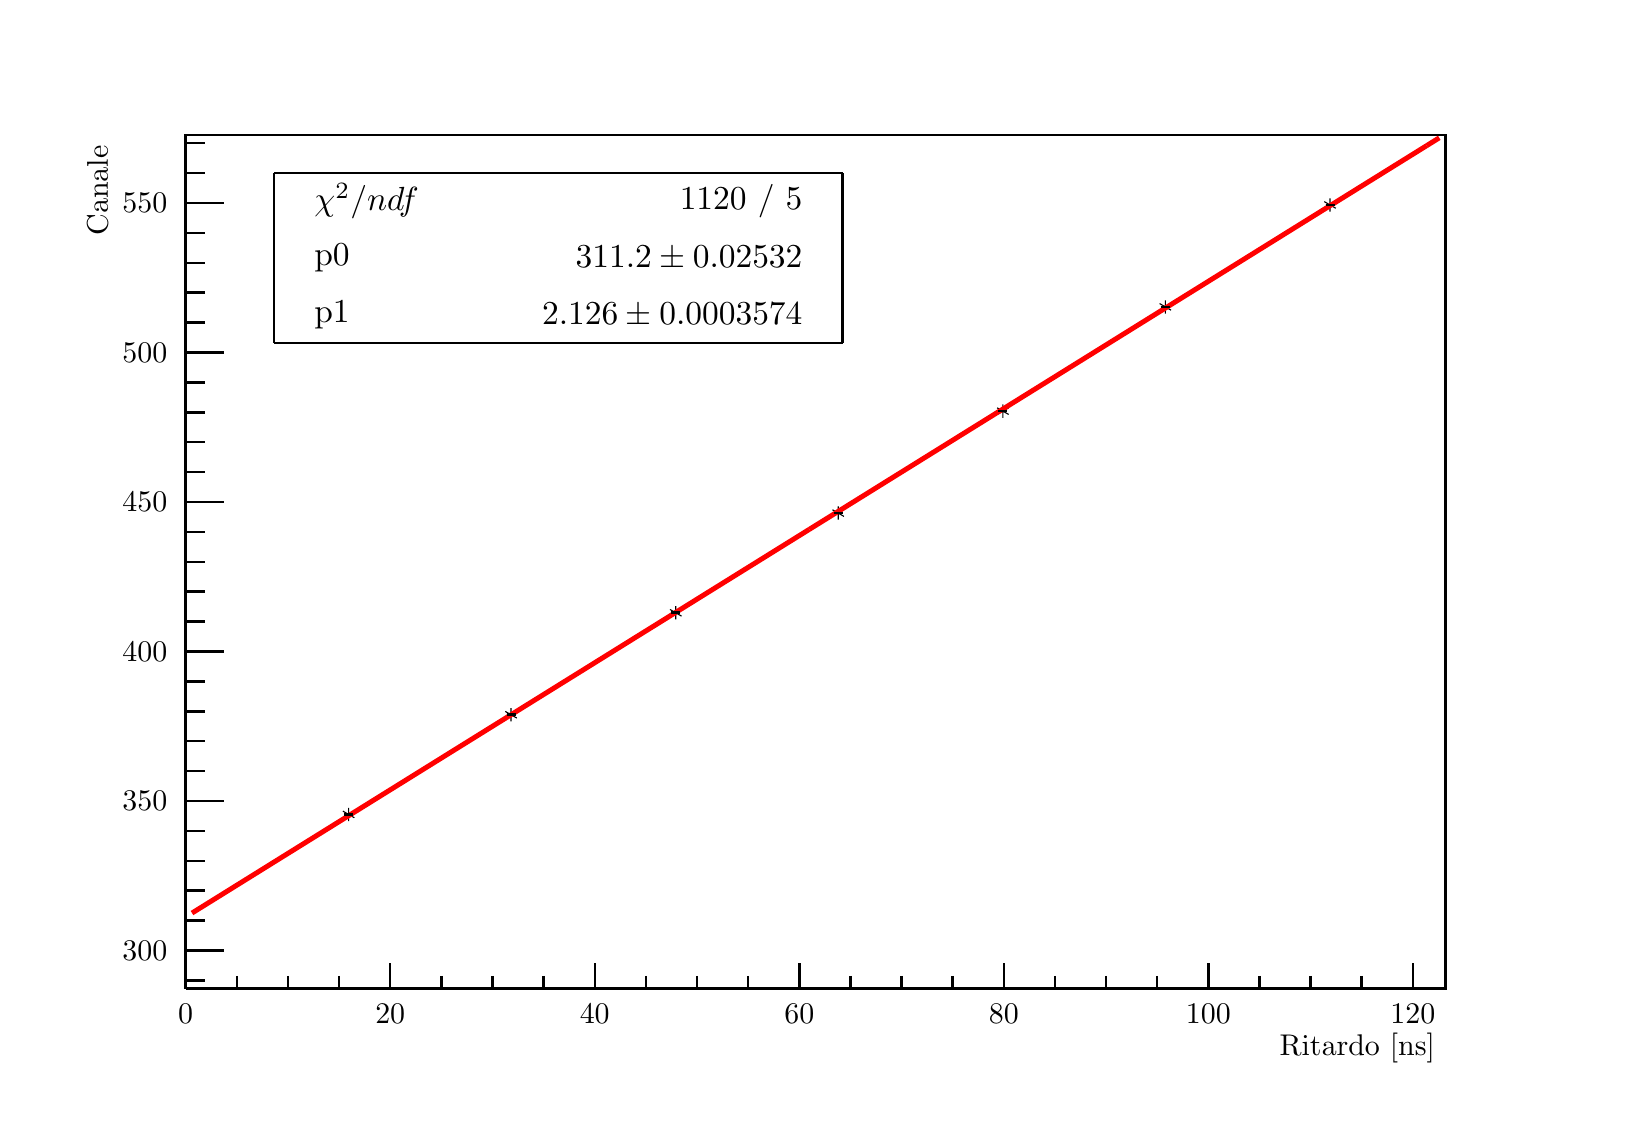
\begin{tikzpicture}
\pgfdeclareplotmark{cross} {
\pgfpathmoveto{\pgfpoint{-0.3\pgfplotmarksize}{\pgfplotmarksize}}
\pgfpathlineto{\pgfpoint{+0.3\pgfplotmarksize}{\pgfplotmarksize}}
\pgfpathlineto{\pgfpoint{+0.3\pgfplotmarksize}{0.3\pgfplotmarksize}}
\pgfpathlineto{\pgfpoint{+1\pgfplotmarksize}{0.3\pgfplotmarksize}}
\pgfpathlineto{\pgfpoint{+1\pgfplotmarksize}{-0.3\pgfplotmarksize}}
\pgfpathlineto{\pgfpoint{+0.3\pgfplotmarksize}{-0.3\pgfplotmarksize}}
\pgfpathlineto{\pgfpoint{+0.3\pgfplotmarksize}{-1.\pgfplotmarksize}}
\pgfpathlineto{\pgfpoint{-0.3\pgfplotmarksize}{-1.\pgfplotmarksize}}
\pgfpathlineto{\pgfpoint{-0.3\pgfplotmarksize}{-0.3\pgfplotmarksize}}
\pgfpathlineto{\pgfpoint{-1.\pgfplotmarksize}{-0.3\pgfplotmarksize}}
\pgfpathlineto{\pgfpoint{-1.\pgfplotmarksize}{0.3\pgfplotmarksize}}
\pgfpathlineto{\pgfpoint{-0.3\pgfplotmarksize}{0.3\pgfplotmarksize}}
\pgfpathclose
\pgfusepathqstroke
}
\pgfdeclareplotmark{cross*} {
\pgfpathmoveto{\pgfpoint{-0.3\pgfplotmarksize}{\pgfplotmarksize}}
\pgfpathlineto{\pgfpoint{+0.3\pgfplotmarksize}{\pgfplotmarksize}}
\pgfpathlineto{\pgfpoint{+0.3\pgfplotmarksize}{0.3\pgfplotmarksize}}
\pgfpathlineto{\pgfpoint{+1\pgfplotmarksize}{0.3\pgfplotmarksize}}
\pgfpathlineto{\pgfpoint{+1\pgfplotmarksize}{-0.3\pgfplotmarksize}}
\pgfpathlineto{\pgfpoint{+0.3\pgfplotmarksize}{-0.3\pgfplotmarksize}}
\pgfpathlineto{\pgfpoint{+0.3\pgfplotmarksize}{-1.\pgfplotmarksize}}
\pgfpathlineto{\pgfpoint{-0.3\pgfplotmarksize}{-1.\pgfplotmarksize}}
\pgfpathlineto{\pgfpoint{-0.3\pgfplotmarksize}{-0.3\pgfplotmarksize}}
\pgfpathlineto{\pgfpoint{-1.\pgfplotmarksize}{-0.3\pgfplotmarksize}}
\pgfpathlineto{\pgfpoint{-1.\pgfplotmarksize}{0.3\pgfplotmarksize}}
\pgfpathlineto{\pgfpoint{-0.3\pgfplotmarksize}{0.3\pgfplotmarksize}}
\pgfpathclose
\pgfusepathqfillstroke
}
\pgfdeclareplotmark{newstar} {
\pgfpathmoveto{\pgfqpoint{0pt}{\pgfplotmarksize}}
\pgfpathlineto{\pgfqpointpolar{44}{0.5\pgfplotmarksize}}
\pgfpathlineto{\pgfqpointpolar{18}{\pgfplotmarksize}}
\pgfpathlineto{\pgfqpointpolar{-20}{0.5\pgfplotmarksize}}
\pgfpathlineto{\pgfqpointpolar{-54}{\pgfplotmarksize}}
\pgfpathlineto{\pgfqpointpolar{-90}{0.5\pgfplotmarksize}}
\pgfpathlineto{\pgfqpointpolar{234}{\pgfplotmarksize}}
\pgfpathlineto{\pgfqpointpolar{198}{0.5\pgfplotmarksize}}
\pgfpathlineto{\pgfqpointpolar{162}{\pgfplotmarksize}}
\pgfpathlineto{\pgfqpointpolar{134}{0.5\pgfplotmarksize}}
\pgfpathclose
\pgfusepathqstroke
}
\pgfdeclareplotmark{newstar*} {
\pgfpathmoveto{\pgfqpoint{0pt}{\pgfplotmarksize}}
\pgfpathlineto{\pgfqpointpolar{44}{0.5\pgfplotmarksize}}
\pgfpathlineto{\pgfqpointpolar{18}{\pgfplotmarksize}}
\pgfpathlineto{\pgfqpointpolar{-20}{0.5\pgfplotmarksize}}
\pgfpathlineto{\pgfqpointpolar{-54}{\pgfplotmarksize}}
\pgfpathlineto{\pgfqpointpolar{-90}{0.5\pgfplotmarksize}}
\pgfpathlineto{\pgfqpointpolar{234}{\pgfplotmarksize}}
\pgfpathlineto{\pgfqpointpolar{198}{0.5\pgfplotmarksize}}
\pgfpathlineto{\pgfqpointpolar{162}{\pgfplotmarksize}}
\pgfpathlineto{\pgfqpointpolar{134}{0.5\pgfplotmarksize}}
\pgfpathclose
\pgfusepathqfillstroke
}
\definecolor{c}{rgb}{1,1,1};
\draw [color=c, fill=c] (0,0) rectangle (20,13.553);
\draw [color=c, fill=c] (2,1.3553) rectangle (18,12.1977);
\definecolor{c}{rgb}{0,0,0};
\draw [c,line width=0.9] (2,1.3553) -- (2,12.1977) -- (18,12.1977) -- (18,1.3553) -- (2,1.3553);
\definecolor{c}{rgb}{1,1,1};
\draw [color=c, fill=c] (2,1.3553) rectangle (18,12.1977);
\definecolor{c}{rgb}{0,0,0};
\draw [c,line width=0.9] (2,1.3553) -- (2,12.1977) -- (18,12.1977) -- (18,1.3553) -- (2,1.3553);
\draw [c,line width=0.9] (2,1.3553) -- (18,1.3553);
\draw [anchor= east] (18,0.596332) node[scale=1.08185, color=c, rotate=0]{Ritardo [ns]};
\draw [c,line width=0.9] (2,1.68057) -- (2,1.3553);
\draw [c,line width=0.9] (2.64935,1.51794) -- (2.64935,1.3553);
\draw [c,line width=0.9] (3.2987,1.51794) -- (3.2987,1.3553);
\draw [c,line width=0.9] (3.94805,1.51794) -- (3.94805,1.3553);
\draw [c,line width=0.9] (4.5974,1.68057) -- (4.5974,1.3553);
\draw [c,line width=0.9] (5.24675,1.51794) -- (5.24675,1.3553);
\draw [c,line width=0.9] (5.8961,1.51794) -- (5.8961,1.3553);
\draw [c,line width=0.9] (6.54545,1.51794) -- (6.54545,1.3553);
\draw [c,line width=0.9] (7.19481,1.68057) -- (7.19481,1.3553);
\draw [c,line width=0.9] (7.84416,1.51794) -- (7.84416,1.3553);
\draw [c,line width=0.9] (8.49351,1.51794) -- (8.49351,1.3553);
\draw [c,line width=0.9] (9.14286,1.51794) -- (9.14286,1.3553);
\draw [c,line width=0.9] (9.79221,1.68057) -- (9.79221,1.3553);
\draw [c,line width=0.9] (10.4416,1.51794) -- (10.4416,1.3553);
\draw [c,line width=0.9] (11.0909,1.51794) -- (11.0909,1.3553);
\draw [c,line width=0.9] (11.7403,1.51794) -- (11.7403,1.3553);
\draw [c,line width=0.9] (12.3896,1.68057) -- (12.3896,1.3553);
\draw [c,line width=0.9] (13.039,1.51794) -- (13.039,1.3553);
\draw [c,line width=0.9] (13.6883,1.51794) -- (13.6883,1.3553);
\draw [c,line width=0.9] (14.3377,1.51794) -- (14.3377,1.3553);
\draw [c,line width=0.9] (14.987,1.68057) -- (14.987,1.3553);
\draw [c,line width=0.9] (15.6364,1.51794) -- (15.6364,1.3553);
\draw [c,line width=0.9] (16.2857,1.51794) -- (16.2857,1.3553);
\draw [c,line width=0.9] (16.9351,1.51794) -- (16.9351,1.3553);
\draw [c,line width=0.9] (17.5844,1.68057) -- (17.5844,1.3553);
\draw [c,line width=0.9] (17.5844,1.68057) -- (17.5844,1.3553);
\draw [anchor=base] (2,0.908052) node[scale=1.08185, color=c, rotate=0]{0};
\draw [anchor=base] (4.5974,0.908052) node[scale=1.08185, color=c, rotate=0]{20};
\draw [anchor=base] (7.19481,0.908052) node[scale=1.08185, color=c, rotate=0]{40};
\draw [anchor=base] (9.79221,0.908052) node[scale=1.08185, color=c, rotate=0]{60};
\draw [anchor=base] (12.3896,0.908052) node[scale=1.08185, color=c, rotate=0]{80};
\draw [anchor=base] (14.987,0.908052) node[scale=1.08185, color=c, rotate=0]{100};
\draw [anchor=base] (17.5844,0.908052) node[scale=1.08185, color=c, rotate=0]{120};
\draw [c,line width=0.9] (2,1.3553) -- (2,12.1977);
\draw [anchor= east] (0.88,12.1977) node[scale=1.08185, color=c, rotate=90]{Canale};
\draw [c,line width=0.9] (2.48,1.83997) -- (2,1.83997);
\draw [c,line width=0.9] (2.24,2.21972) -- (2,2.21972);
\draw [c,line width=0.9] (2.24,2.59947) -- (2,2.59947);
\draw [c,line width=0.9] (2.24,2.97922) -- (2,2.97922);
\draw [c,line width=0.9] (2.24,3.35896) -- (2,3.35896);
\draw [c,line width=0.9] (2.48,3.73871) -- (2,3.73871);
\draw [c,line width=0.9] (2.24,4.11846) -- (2,4.11846);
\draw [c,line width=0.9] (2.24,4.49821) -- (2,4.49821);
\draw [c,line width=0.9] (2.24,4.87796) -- (2,4.87796);
\draw [c,line width=0.9] (2.24,5.2577) -- (2,5.2577);
\draw [c,line width=0.9] (2.48,5.63745) -- (2,5.63745);
\draw [c,line width=0.9] (2.24,6.0172) -- (2,6.0172);
\draw [c,line width=0.9] (2.24,6.39695) -- (2,6.39695);
\draw [c,line width=0.9] (2.24,6.77669) -- (2,6.77669);
\draw [c,line width=0.9] (2.24,7.15644) -- (2,7.15644);
\draw [c,line width=0.9] (2.48,7.53619) -- (2,7.53619);
\draw [c,line width=0.9] (2.24,7.91594) -- (2,7.91594);
\draw [c,line width=0.9] (2.24,8.29569) -- (2,8.29569);
\draw [c,line width=0.9] (2.24,8.67543) -- (2,8.67543);
\draw [c,line width=0.9] (2.24,9.05518) -- (2,9.05518);
\draw [c,line width=0.9] (2.48,9.43493) -- (2,9.43493);
\draw [c,line width=0.9] (2.24,9.81468) -- (2,9.81468);
\draw [c,line width=0.9] (2.24,10.1944) -- (2,10.1944);
\draw [c,line width=0.9] (2.24,10.5742) -- (2,10.5742);
\draw [c,line width=0.9] (2.24,10.9539) -- (2,10.9539);
\draw [c,line width=0.9] (2.48,11.3337) -- (2,11.3337);
\draw [c,line width=0.9] (2.48,1.83997) -- (2,1.83997);
\draw [c,line width=0.9] (2.24,1.46023) -- (2,1.46023);
\draw [c,line width=0.9] (2.48,11.3337) -- (2,11.3337);
\draw [c,line width=0.9] (2.24,11.7134) -- (2,11.7134);
\draw [c,line width=0.9] (2.24,12.0932) -- (2,12.0932);
\draw [anchor= east] (1.9,1.83997) node[scale=1.08185, color=c, rotate=0]{300};
\draw [anchor= east] (1.9,3.73871) node[scale=1.08185, color=c, rotate=0]{350};
\draw [anchor= east] (1.9,5.63745) node[scale=1.08185, color=c, rotate=0]{400};
\draw [anchor= east] (1.9,7.53619) node[scale=1.08185, color=c, rotate=0]{450};
\draw [anchor= east] (1.9,9.43493) node[scale=1.08185, color=c, rotate=0]{500};
\draw [anchor= east] (1.9,11.3337) node[scale=1.08185, color=c, rotate=0]{550};
\definecolor{c}{rgb}{1,1,1};
\draw [color=c, fill=c] (3.12321,9.55329) rectangle (10.3438,11.7114);
\definecolor{c}{rgb}{0,0,0};
\draw [c,line width=0.9] (3.12321,9.55329) -- (10.3438,9.55329);
\draw [c,line width=0.9] (10.3438,9.55329) -- (10.3438,11.7114);
\draw [c,line width=0.9] (10.3438,11.7114) -- (3.12321,11.7114);
\draw [c,line width=0.9] (3.12321,11.7114) -- (3.12321,9.55329);
\draw [anchor= west] (3.48424,11.3517) node[scale=1.20912, color=c, rotate=0]{$\chi^{2} / ndf $};
\draw [anchor= east] (9.98281,11.3517) node[scale=1.20912, color=c, rotate=0]{  1120 / 5};
\draw [anchor= west] (3.48424,10.6323) node[scale=1.20912, color=c, rotate=0]{p0       };
\draw [anchor= east] (9.98281,10.6323) node[scale=1.20912, color=c, rotate=0]{$ 311.2 \pm 0.02532$};
\draw [anchor= west] (3.48424,9.91298) node[scale=1.20912, color=c, rotate=0]{p1       };
\draw [anchor= east] (9.98281,9.91298) node[scale=1.20912, color=c, rotate=0]{$ 2.126 \pm 0.0003574$};
\foreach \P in {(4.06877,3.5681), (6.13181,4.83419), (8.2235,6.12907), (10.2865,7.39517), (12.3782,8.69004), (14.4413,10.0137), (16.5329,11.3086)}{\draw[mark options={color=c,fill=c},mark size=2.402402pt,mark=asterisk] plot coordinates {\P};}
\definecolor{c}{rgb}{1,0,0};
\draw [c,line width=1.8] (2.08,2.31566) -- (2.24,2.4151) -- (2.4,2.51455) -- (2.56,2.614) -- (2.72,2.71345) -- (2.88,2.81289) -- (3.04,2.91234) -- (3.2,3.01179) -- (3.36,3.11123) -- (3.52,3.21068) -- (3.68,3.31013) -- (3.84,3.40958) -- (4,3.50902) --
 (4.16,3.60847) -- (4.32,3.70792) -- (4.48,3.80737) -- (4.64,3.90681) -- (4.8,4.00626) -- (4.96,4.10571) -- (5.12,4.20516) -- (5.28,4.3046) -- (5.44,4.40405) -- (5.6,4.5035) -- (5.76,4.60295) -- (5.92,4.70239) -- (6.08,4.80184) -- (6.24,4.90129) --
 (6.4,5.00073) -- (6.56,5.10018) -- (6.72,5.19963) -- (6.88,5.29908) -- (7.04,5.39852) -- (7.2,5.49797) -- (7.36,5.59742) -- (7.52,5.69687) -- (7.68,5.79631) -- (7.84,5.89576) -- (8,5.99521) -- (8.16,6.09466) -- (8.32,6.1941) -- (8.48,6.29355) --
 (8.64,6.393) -- (8.8,6.49244) -- (8.96,6.59189) -- (9.12,6.69134) -- (9.28,6.79079) -- (9.44,6.89023) -- (9.6,6.98968) -- (9.76,7.08913) -- (9.92,7.18858);
\draw [c,line width=1.8] (9.92,7.18858) -- (10.08,7.28802) -- (10.24,7.38747) -- (10.4,7.48692) -- (10.56,7.58637) -- (10.72,7.68581) -- (10.88,7.78526) -- (11.04,7.88471) -- (11.2,7.98416) -- (11.36,8.0836) -- (11.52,8.18305) -- (11.68,8.2825) --
 (11.84,8.38194) -- (12,8.48139) -- (12.16,8.58084) -- (12.32,8.68029) -- (12.48,8.77973) -- (12.64,8.87918) -- (12.8,8.97863) -- (12.96,9.07808) -- (13.12,9.17752) -- (13.28,9.27697) -- (13.44,9.37642) -- (13.6,9.47587) -- (13.76,9.57531) --
 (13.92,9.67476) -- (14.08,9.77421) -- (14.24,9.87366) -- (14.4,9.9731) -- (14.56,10.0725) -- (14.72,10.172) -- (14.88,10.2714) -- (15.04,10.3709) -- (15.2,10.4703) -- (15.36,10.5698) -- (15.52,10.6692) -- (15.68,10.7687) -- (15.84,10.8681) --
 (16,10.9676) -- (16.16,11.067) -- (16.32,11.1665) -- (16.48,11.2659) -- (16.64,11.3654) -- (16.8,11.4648) -- (16.96,11.5643) -- (17.12,11.6637) -- (17.28,11.7632) -- (17.44,11.8626) -- (17.6,11.962) -- (17.76,12.0615);
\draw [c,line width=1.8] (17.76,12.0615) -- (17.92,12.1609);
\definecolor{c}{rgb}{1,1,1};
\draw [color=c, fill=c] (3.12321,9.55329) rectangle (10.3438,11.7114);
\definecolor{c}{rgb}{0,0,0};
\draw [c,line width=0.9] (3.12321,9.55329) -- (10.3438,9.55329);
\draw [c,line width=0.9] (10.3438,9.55329) -- (10.3438,11.7114);
\draw [c,line width=0.9] (10.3438,11.7114) -- (3.12321,11.7114);
\draw [c,line width=0.9] (3.12321,11.7114) -- (3.12321,9.55329);
\draw [anchor= west] (3.48424,11.3517) node[scale=1.20912, color=c, rotate=0]{$\chi^{2} / ndf $};
\draw [anchor= east] (9.98281,11.3517) node[scale=1.20912, color=c, rotate=0]{  1120 / 5};
\draw [anchor= west] (3.48424,10.6323) node[scale=1.20912, color=c, rotate=0]{p0       };
\draw [anchor= east] (9.98281,10.6323) node[scale=1.20912, color=c, rotate=0]{$ 311.2 \pm 0.02532$};
\draw [anchor= west] (3.48424,9.91298) node[scale=1.20912, color=c, rotate=0]{p1       };
\draw [anchor= east] (9.98281,9.91298) node[scale=1.20912, color=c, rotate=0]{$ 2.126 \pm 0.0003574$};
\draw [c,line width=0.9] (4.06877,3.5681) -- (4.06877,3.56923);
\draw [c,line width=0.9] (4.01146,3.56923) -- (4.12607,3.56923);
\draw [c,line width=0.9] (4.06877,3.5681) -- (4.06877,3.56696);
\draw [c,line width=0.9] (4.01146,3.56696) -- (4.12607,3.56696);
\draw [c,line width=0.9] (6.13181,4.83419) -- (6.13181,4.83533);
\draw [c,line width=0.9] (6.0745,4.83533) -- (6.18911,4.83533);
\draw [c,line width=0.9] (6.13181,4.83419) -- (6.13181,4.83305);
\draw [c,line width=0.9] (6.0745,4.83305) -- (6.18911,4.83305);
\draw [c,line width=0.9] (8.2235,6.12907) -- (8.2235,6.13021);
\draw [c,line width=0.9] (8.16619,6.13021) -- (8.2808,6.13021);
\draw [c,line width=0.9] (8.2235,6.12907) -- (8.2235,6.12793);
\draw [c,line width=0.9] (8.16619,6.12793) -- (8.2808,6.12793);
\draw [c,line width=0.9] (10.2865,7.39517) -- (10.2865,7.39631);
\draw [c,line width=0.9] (10.2292,7.39631) -- (10.3438,7.39631);
\draw [c,line width=0.9] (10.2865,7.39517) -- (10.2865,7.39403);
\draw [c,line width=0.9] (10.2292,7.39403) -- (10.3438,7.39403);
\draw [c,line width=0.9] (12.3782,8.69004) -- (12.3782,8.69156);
\draw [c,line width=0.9] (12.3209,8.69156) -- (12.4355,8.69156);
\draw [c,line width=0.9] (12.3782,8.69004) -- (12.3782,8.68852);
\draw [c,line width=0.9] (12.3209,8.68852) -- (12.4355,8.68852);
\draw [c,line width=0.9] (14.4413,10.0137) -- (14.4413,10.0148);
\draw [c,line width=0.9] (14.384,10.0148) -- (14.4986,10.0148);
\draw [c,line width=0.9] (14.4413,10.0137) -- (14.4413,10.0125);
\draw [c,line width=0.9] (14.384,10.0125) -- (14.4986,10.0125);
\draw [c,line width=0.9] (16.5329,11.3086) -- (16.5329,11.3097);
\draw [c,line width=0.9] (16.4756,11.3097) -- (16.5903,11.3097);
\draw [c,line width=0.9] (16.5329,11.3086) -- (16.5329,11.3074);
\draw [c,line width=0.9] (16.4756,11.3074) -- (16.5903,11.3074);
\end{tikzpicture}

%Inserire regressione lineare della calibrazione temporale dell'apparato strumentale

\FloatBarrier
\subsection{Decadimento a due o tre fotoni}

Una volta calibrato tutto il sistema di acquisizione, si è arrivati al vero e proprio studio del positronio: in particolare si vuole misurare il rapporto tra il decadimento
a due e a tre fotoni del positronio e la distribuzione temporale degli eventi.\\

Per studiare la probabilità di decadimento è stato sufficiente prendere i dati analizzati e considerare il dead time dei rivelatori: 
